% Options for packages loaded elsewhere
\PassOptionsToPackage{unicode}{hyperref}
\PassOptionsToPackage{hyphens}{url}
%
\documentclass[
  11pt,
]{book}
\usepackage{amsmath,amssymb}
\usepackage{iftex}
\ifPDFTeX
  \usepackage[T1]{fontenc}
  \usepackage[utf8]{inputenc}
  \usepackage{textcomp} % provide euro and other symbols
\else % if luatex or xetex
  \usepackage{unicode-math} % this also loads fontspec
  \defaultfontfeatures{Scale=MatchLowercase}
  \defaultfontfeatures[\rmfamily]{Ligatures=TeX,Scale=1}
\fi
\usepackage{lmodern}
\ifPDFTeX\else
  % xetex/luatex font selection
\fi
% Use upquote if available, for straight quotes in verbatim environments
\IfFileExists{upquote.sty}{\usepackage{upquote}}{}
\IfFileExists{microtype.sty}{% use microtype if available
  \usepackage[]{microtype}
  \UseMicrotypeSet[protrusion]{basicmath} % disable protrusion for tt fonts
}{}
\makeatletter
\@ifundefined{KOMAClassName}{% if non-KOMA class
  \IfFileExists{parskip.sty}{%
    \usepackage{parskip}
  }{% else
    \setlength{\parindent}{0pt}
    \setlength{\parskip}{6pt plus 2pt minus 1pt}}
}{% if KOMA class
  \KOMAoptions{parskip=half}}
\makeatother
\usepackage{xcolor}
\usepackage[margin=1in]{geometry}
\usepackage{color}
\usepackage{fancyvrb}
\newcommand{\VerbBar}{|}
\newcommand{\VERB}{\Verb[commandchars=\\\{\}]}
\DefineVerbatimEnvironment{Highlighting}{Verbatim}{commandchars=\\\{\}}
% Add ',fontsize=\small' for more characters per line
\usepackage{framed}
\definecolor{shadecolor}{RGB}{248,248,248}
\newenvironment{Shaded}{\begin{snugshade}}{\end{snugshade}}
\newcommand{\AlertTok}[1]{\textcolor[rgb]{0.94,0.16,0.16}{#1}}
\newcommand{\AnnotationTok}[1]{\textcolor[rgb]{0.56,0.35,0.01}{\textbf{\textit{#1}}}}
\newcommand{\AttributeTok}[1]{\textcolor[rgb]{0.13,0.29,0.53}{#1}}
\newcommand{\BaseNTok}[1]{\textcolor[rgb]{0.00,0.00,0.81}{#1}}
\newcommand{\BuiltInTok}[1]{#1}
\newcommand{\CharTok}[1]{\textcolor[rgb]{0.31,0.60,0.02}{#1}}
\newcommand{\CommentTok}[1]{\textcolor[rgb]{0.56,0.35,0.01}{\textit{#1}}}
\newcommand{\CommentVarTok}[1]{\textcolor[rgb]{0.56,0.35,0.01}{\textbf{\textit{#1}}}}
\newcommand{\ConstantTok}[1]{\textcolor[rgb]{0.56,0.35,0.01}{#1}}
\newcommand{\ControlFlowTok}[1]{\textcolor[rgb]{0.13,0.29,0.53}{\textbf{#1}}}
\newcommand{\DataTypeTok}[1]{\textcolor[rgb]{0.13,0.29,0.53}{#1}}
\newcommand{\DecValTok}[1]{\textcolor[rgb]{0.00,0.00,0.81}{#1}}
\newcommand{\DocumentationTok}[1]{\textcolor[rgb]{0.56,0.35,0.01}{\textbf{\textit{#1}}}}
\newcommand{\ErrorTok}[1]{\textcolor[rgb]{0.64,0.00,0.00}{\textbf{#1}}}
\newcommand{\ExtensionTok}[1]{#1}
\newcommand{\FloatTok}[1]{\textcolor[rgb]{0.00,0.00,0.81}{#1}}
\newcommand{\FunctionTok}[1]{\textcolor[rgb]{0.13,0.29,0.53}{\textbf{#1}}}
\newcommand{\ImportTok}[1]{#1}
\newcommand{\InformationTok}[1]{\textcolor[rgb]{0.56,0.35,0.01}{\textbf{\textit{#1}}}}
\newcommand{\KeywordTok}[1]{\textcolor[rgb]{0.13,0.29,0.53}{\textbf{#1}}}
\newcommand{\NormalTok}[1]{#1}
\newcommand{\OperatorTok}[1]{\textcolor[rgb]{0.81,0.36,0.00}{\textbf{#1}}}
\newcommand{\OtherTok}[1]{\textcolor[rgb]{0.56,0.35,0.01}{#1}}
\newcommand{\PreprocessorTok}[1]{\textcolor[rgb]{0.56,0.35,0.01}{\textit{#1}}}
\newcommand{\RegionMarkerTok}[1]{#1}
\newcommand{\SpecialCharTok}[1]{\textcolor[rgb]{0.81,0.36,0.00}{\textbf{#1}}}
\newcommand{\SpecialStringTok}[1]{\textcolor[rgb]{0.31,0.60,0.02}{#1}}
\newcommand{\StringTok}[1]{\textcolor[rgb]{0.31,0.60,0.02}{#1}}
\newcommand{\VariableTok}[1]{\textcolor[rgb]{0.00,0.00,0.00}{#1}}
\newcommand{\VerbatimStringTok}[1]{\textcolor[rgb]{0.31,0.60,0.02}{#1}}
\newcommand{\WarningTok}[1]{\textcolor[rgb]{0.56,0.35,0.01}{\textbf{\textit{#1}}}}
\usepackage{longtable,booktabs,array}
\usepackage{calc} % for calculating minipage widths
% Correct order of tables after \paragraph or \subparagraph
\usepackage{etoolbox}
\makeatletter
\patchcmd\longtable{\par}{\if@noskipsec\mbox{}\fi\par}{}{}
\makeatother
% Allow footnotes in longtable head/foot
\IfFileExists{footnotehyper.sty}{\usepackage{footnotehyper}}{\usepackage{footnote}}
\makesavenoteenv{longtable}
\usepackage{graphicx}
\makeatletter
\def\maxwidth{\ifdim\Gin@nat@width>\linewidth\linewidth\else\Gin@nat@width\fi}
\def\maxheight{\ifdim\Gin@nat@height>\textheight\textheight\else\Gin@nat@height\fi}
\makeatother
% Scale images if necessary, so that they will not overflow the page
% margins by default, and it is still possible to overwrite the defaults
% using explicit options in \includegraphics[width, height, ...]{}
\setkeys{Gin}{width=\maxwidth,height=\maxheight,keepaspectratio}
% Set default figure placement to htbp
\makeatletter
\def\fps@figure{htbp}
\makeatother
\setlength{\emergencystretch}{3em} % prevent overfull lines
\providecommand{\tightlist}{%
  \setlength{\itemsep}{0pt}\setlength{\parskip}{0pt}}
\setcounter{secnumdepth}{5}
\usepackage{booktabs}
\usepackage{amsthm}
\usepackage{fvextra} \DefineVerbatimEnvironment{Highlighting}{Verbatim}{breaklines,breaksymbol=,commandchars=\\\{\}}
\usepackage{booktabs}
\usepackage{longtable}
\usepackage{array}
\usepackage{multirow}
\usepackage{wrapfig}
\usepackage{float}
\usepackage{colortbl}
\usepackage{pdflscape}
\usepackage{tabu}
\usepackage{threeparttable}
\usepackage{threeparttablex}
\usepackage[normalem]{ulem}
\usepackage{makecell}
\usepackage{xcolor}
\ifLuaTeX
  \usepackage{selnolig}  % disable illegal ligatures
\fi
\usepackage[]{natbib}
\bibliographystyle{plainnat}
\IfFileExists{bookmark.sty}{\usepackage{bookmark}}{\usepackage{hyperref}}
\IfFileExists{xurl.sty}{\usepackage{xurl}}{} % add URL line breaks if available
\urlstyle{same}
\hypersetup{
  pdftitle={Sports Analytics},
  pdfauthor={Aaron Nielsen, Department of Statistics, Colorado State University},
  hidelinks,
  pdfcreator={LaTeX via pandoc}}

\title{Sports Analytics}
\author{Aaron Nielsen, Department of Statistics, Colorado State University}
\date{2024-02-20}

\usepackage{amsthm}
\newtheorem{theorem}{Theorem}[chapter]
\newtheorem{lemma}{Lemma}[chapter]
\newtheorem{corollary}{Corollary}[chapter]
\newtheorem{proposition}{Proposition}[chapter]
\newtheorem{conjecture}{Conjecture}[chapter]
\theoremstyle{definition}
\newtheorem{definition}{Definition}[chapter]
\theoremstyle{definition}
\newtheorem{example}{Example}[chapter]
\theoremstyle{definition}
\newtheorem{exercise}{Exercise}[chapter]
\theoremstyle{definition}
\newtheorem{hypothesis}{Hypothesis}[chapter]
\theoremstyle{remark}
\newtheorem*{remark}{Remark}
\newtheorem*{solution}{Solution}
\begin{document}
\maketitle

{
\setcounter{tocdepth}{1}
\tableofcontents
}
\hypertarget{about}{%
\chapter*{About}\label{about}}
\addcontentsline{toc}{chapter}{About}

This book serves as the course textbook for the following courses at Colorado State University:

\begin{itemize}
\item
  STAT 351 (Sports Statistics and Analytics I)
\item
  STAT 451 (Sports Statistics and Analytics II)
\end{itemize}

\hfill\break

CSU students contributed to the creation of this book. Many thanks to the following student collaborators: Levi Kipp, Ellie Martinez, Isaac Moorman, Connor Gibbs, Brayden Look

\hypertarget{preliminaries}{%
\chapter*{Preliminaries}\label{preliminaries}}
\addcontentsline{toc}{chapter}{Preliminaries}

\hypertarget{getting-started-with-r}{%
\section*{Getting Started With R}\label{getting-started-with-r}}
\addcontentsline{toc}{section}{Getting Started With R}

\hypertarget{installing-r}{%
\subsection*{Installing R}\label{installing-r}}
\addcontentsline{toc}{subsection}{Installing R}

For this class, you will be using R Studio to complete statistical analyses on your computer.

To begin using R Studio, you will need to install ``R'' first and then install ``R Studio'' on your computer.

\textbf{\emph{Step 1: Download R}}\\
(a) Visit \url{https://www.r-project.org/}\\
(b) Click \textbf{CRAN} under \textbf{Download}
(c) Select any of the mirrors\\
(d) Click the appropriate link for your type of system (Mac, Windows, Linux)\\
(e) Download R on this next page.\\
(For Windows, this will say \textbf{install R for the first time}. For Mac, this will be under \textbf{Latest release} and will be something like \textbf{R-4.1.0.pkg} -- the numbers may differ depending on the most recent version)\\
(f) Install R on your computer\\

\textbf{\emph{Step 2: Download R Studio}}\\
(a) Visit \url{https://www.rstudio.com/products/rstudio/download/\#download}\\
(b) Click to download\\
(c) Install R Studio on your computer\\

\newpage

\textbf{\emph{Step 3: Verify R Studio is working}}\\
(a) Open R Studio\\
(b) Let's enter a small dataset and calculate the average to make sure everything is working correctly.\\
(c) In the console, type in the following dataset of Sammy Sosa's season home run totals from 1998--2002:\\

\begin{Shaded}
\begin{Highlighting}[]
\NormalTok{sosa.HR }\OtherTok{\textless{}{-}} \FunctionTok{c}\NormalTok{(}\DecValTok{66}\NormalTok{,}\DecValTok{63}\NormalTok{,}\DecValTok{50}\NormalTok{,}\DecValTok{64}\NormalTok{,}\DecValTok{49}\NormalTok{)}
\end{Highlighting}
\end{Shaded}

\begin{enumerate}
\def\labelenumi{(\alph{enumi})}
\setcounter{enumi}{3}
\tightlist
\item
  In the console, calculate the average season home run total for Sammy Sosa between 1998--2002:\\
\end{enumerate}

\begin{Shaded}
\begin{Highlighting}[]
\FunctionTok{mean}\NormalTok{(sosa.HR)}
\end{Highlighting}
\end{Shaded}

\begin{verbatim}
## [1] 58.4
\end{verbatim}

\noindent (e) Did you find Slammin' Sammy's average home run total from 1998--2002 was 58.4? If so, you should be set up correctly!

\newpage

\hypertarget{some-r-basics}{%
\subsection*{Some R Basics}\label{some-r-basics}}
\addcontentsline{toc}{subsection}{Some R Basics}

For the following examples, let's consider Peyton Manning's career with the Denver Broncos. In his four seasons with the Broncos, Manning's passing yard totals were: 4659, 5477, 4727, 2249. Let's enter this data into R. To enter a vector of data, use the \textbf{c()} function.

\begin{Shaded}
\begin{Highlighting}[]
\NormalTok{peyton }\OtherTok{\textless{}{-}} \FunctionTok{c}\NormalTok{(}\DecValTok{4659}\NormalTok{, }\DecValTok{5477}\NormalTok{, }\DecValTok{4727}\NormalTok{, }\DecValTok{2249}\NormalTok{)}
\end{Highlighting}
\end{Shaded}

To look at the data you just put in the variable \emph{peyton}, type \emph{peyton} into the console and press enter.

\begin{Shaded}
\begin{Highlighting}[]
\NormalTok{peyton}
\end{Highlighting}
\end{Shaded}

\begin{verbatim}
## [1] 4659 5477 4727 2249
\end{verbatim}

Some basic function for calculating summary statistics include \textbf{summary}, \textbf{mean()}, \textbf{median()}, \textbf{var()}, and \textbf{sd()}.

\begin{Shaded}
\begin{Highlighting}[]
\FunctionTok{summary}\NormalTok{(peyton)}
\end{Highlighting}
\end{Shaded}

\begin{verbatim}
##    Min. 1st Qu.  Median    Mean 3rd Qu.    Max. 
##    2249    4056    4693    4278    4914    5477
\end{verbatim}

\begin{Shaded}
\begin{Highlighting}[]
\FunctionTok{mean}\NormalTok{(peyton)}
\end{Highlighting}
\end{Shaded}

\begin{verbatim}
## [1] 4278
\end{verbatim}

\begin{Shaded}
\begin{Highlighting}[]
\FunctionTok{sd}\NormalTok{(peyton)}
\end{Highlighting}
\end{Shaded}

\begin{verbatim}
## [1] 1402.522
\end{verbatim}

R allows you to install additional packages (collections of functions) that aren't offered in the base version of R. To install a package, use \textbf{install.packages()} and to load a package, use \textbf{library()}.

One package that we will use frequently is \textbf{tidyverse}. This package includes several other packages and functions such as \textbf{ggplot} (plotting function), \textbf{dplyr} (data manipulation package), and \textbf{stringr} (string manipulation package).

\begin{Shaded}
\begin{Highlighting}[]
\FunctionTok{install.packages}\NormalTok{(}\StringTok{"tidyverse"}\NormalTok{)}
\FunctionTok{library}\NormalTok{(}\StringTok{"tidyverse"}\NormalTok{)}
\end{Highlighting}
\end{Shaded}

You will also need to know how to load datasets from files. For this class, we will typically provide data files is .csv format.

\newpage

Here is how to load a file:

\begin{Shaded}
\begin{Highlighting}[]
\CommentTok{\# load readr package and load example dataset}
\NormalTok{NFL\_2021\_Team\_Passing }\OtherTok{\textless{}{-}} \FunctionTok{read\_csv}\NormalTok{(}\StringTok{"data/NFL\_2021\_Team\_Passing.csv"}\NormalTok{)}

\CommentTok{\# we can look at the header (first few entries) using "head()"}
\FunctionTok{head}\NormalTok{(NFL\_2021\_Team\_Passing)}
\end{Highlighting}
\end{Shaded}

\begin{verbatim}
## # A tibble: 6 x 25
##      Rk Tm             G   Cmp   Att `Cmp%`   Yds    TD `TD%`   Int `Int%`   Lng
##   <dbl> <chr>      <dbl> <dbl> <dbl>  <dbl> <dbl> <dbl> <dbl> <dbl>  <dbl> <dbl>
## 1     1 Tampa Bay~    17   492   731   67.3  5229    43   5.9    12    1.6    62
## 2     2 Los Angel~    17   443   674   65.7  4800    38   5.6    15    2.2    72
## 3     3 Dallas Co~    17   444   647   68.6  4800    40   6.2    11    1.7    73
## 4     4 Kansas Ci~    17   448   675   66.4  4791    37   5.5    13    1.9    75
## 5     5 Los Angel~    17   406   607   66.9  4642    41   6.8    18    3      79
## 6     6 Las Vegas~    17   429   628   68.3  4567    23   3.7    14    2.2    61
## # ... with 13 more variables: `Y/A` <dbl>, `AY/A` <dbl>, `Y/C` <dbl>,
## #   `Y/G` <dbl>, Rate <dbl>, Sk <dbl>, SKYds <dbl>, `Sk%` <dbl>, `NY/A` <dbl>,
## #   `ANY/A` <dbl>, `4QC` <dbl>, GWD <dbl>, EXP <dbl>
\end{verbatim}

\newpage

\hypertarget{course-goals}{%
\section*{Course Goals}\label{course-goals}}
\addcontentsline{toc}{section}{Course Goals}

Our course goals include:

\vfill

\hypertarget{which-sports}{%
\section*{Which Sports?}\label{which-sports}}
\addcontentsline{toc}{section}{Which Sports?}

We will be working with data from the following sports:

\vfill

You can optionally investigate data from other sports for your projects such as:

\vfill

\hypertarget{challenges}{%
\section*{Challenges}\label{challenges}}
\addcontentsline{toc}{section}{Challenges}

What kind of challenges could we encounter dealing with sports data?

\vfill

\hypertarget{ethical-concerns}{%
\section*{Ethical Concerns}\label{ethical-concerns}}
\addcontentsline{toc}{section}{Ethical Concerns}

What kinds of ethical concerns should we consider when dealing with sports data?

\vfill

\hypertarget{exploratory-data-analysis}{%
\chapter{Exploratory Data Analysis}\label{exploratory-data-analysis}}

\hypertarget{descriptive-statistics}{%
\section{Descriptive Statistics}\label{descriptive-statistics}}

\hypertarget{definitions}{%
\subsection{Definitions}\label{definitions}}

\begin{definition}
A \textbf{\emph{population}} is a well-defined complete collection of objects.
\end{definition}

\begin{definition}
A \textbf{\emph{sample}} is a subset of the population.
\end{definition}

\begin{example}
Suppose we are interested in studying Peyton's Manning's season passing yards totals. How could you define the population and what is one possible sample?
\end{example}

\vfill

\begin{definition}
\textbf{\emph{Quantitative data}} is numeric data or numbers. It can be broken into two further categories: discrete and continuous data.
\end{definition}

\begin{definition}
\textbf{\emph{Discrete data}} is quantitative data with a finite or countably infinite number of values.
\end{definition}

\begin{definition}
\textbf{\emph{Continuous data}} is quantitative data with an uncountably infinite number of values or data taken from an interval.
\end{definition}

\begin{example}
What are possible discrete and continuous data associated with Peyton Manning?
\end{example}

\vfill

\begin{definition}
\textbf{\emph{Qualitative data}} refers to names, categories, or descriptions. It can also be broken down into
two further categories, nominal data and ordinal data.
\end{definition}

\begin{definition}
\textbf{\emph{Nominal data}} is qualitative data with no natural ordering.
\end{definition}

\begin{definition}
\textbf{\emph{Ordinal data}} is qualitative data with a natural ordering.
\end{definition}

\begin{example}
What are possible nominal and ordinal data associated with Peyton Manning?
\end{example}

\vfill

\newpage

\hypertarget{descriptive-statistics-1}{%
\subsection{Descriptive Statistics}\label{descriptive-statistics-1}}

While we will learn about some descriptive statistics that are unique to specific sports, there are some descriptive statistics that are frequently used in many applications.

\hypertarget{quantitative-data}{%
\subsubsection{Quantitative Data}\label{quantitative-data}}

There are different descriptive statistics depending on the type of data you are analyzing. We will begin by looking at descriptive statistics for quantitative data.

To begin, let \(x_1, x_2, \ldots, x_n\) represent a numerical dataset with a sample of size \(n\), where \(x_i\) is the \(i^\text{th}\) value in the dataset.

\begin{definition}
The \textbf{\emph{sum}} of the data values is given by: \(\sum_{i=1}^n x_i = x_1 + x_2 + \ldots + x_n\)
\end{definition}

\begin{definition}
The \textbf{\emph{sample mean}} (or sample average), \(\bar{x}\), of the numerical dataset is given by \(\bar{x} = \frac{1}{n} \sum_{i=1}^n x_i\)
\end{definition}

\begin{definition}
The \textbf{\emph{population mean}} (or population average), \(\mu\), is the mean value for the entire population.
\end{definition}

The mean can be thought of as a measure of center or more generally, a measure of location.

\begin{example}
Recall that Peyton Manning's season passing yards total while with the Broncos were: 4659, 5477, 4727, 2249. Calculate the sample mean of these values.
\end{example}

\hfill\break
\hfill\break
\hfill\break
\hfill\break
\hfill\break

\begin{Shaded}
\begin{Highlighting}[]
\CommentTok{\# Calculate the sample of Peyton Manning\textquotesingle{}s passing yards season totals with Colts}
\NormalTok{peyton.broncos }\OtherTok{\textless{}{-}} \FunctionTok{c}\NormalTok{(}\DecValTok{4659}\NormalTok{, }\DecValTok{5477}\NormalTok{, }\DecValTok{4727}\NormalTok{, }\DecValTok{2249}\NormalTok{)}
\FunctionTok{mean}\NormalTok{(peyton.broncos)}
\end{Highlighting}
\end{Shaded}

\begin{verbatim}
## [1] 4278
\end{verbatim}

In sports statistics, we often have to choose between using a descriptive statistic that summarizes a quantity versus a descriptive statistic that summarizes a rate. For instance, in basketball, we can compare two players based on how many points they score in a game (total quantity) or we can compare two players based on how many points per minute played (rate statistic). Many applications in sports analytics focus more on rate statistics rather than quantity statistics. Why?

We can measure the spread or variability of a dataset using \emph{variance} and \emph{standard devatiation}.

\begin{definition}
The \textbf{\emph{sample variance}}, \(s^2\), of the numerical dataset is a measure of spread and is given by \(s^2 = \frac{1}{n-1}\sum_{i=1}^n (x_i - \bar{x})^2\)
\end{definition}

\begin{definition}
The \textbf{\emph{sample standard deviation}}, \(s\), of the numerical dataset is a measure of spread and is given by \(s = \sqrt{s^2} = \sqrt{\frac{1}{n-1}\sum_{i=1}^n (x_i - \bar{x})^2}\)
\end{definition}

\begin{definition}
The \textbf{\emph{population variance}}, \(\sigma^2\), is the variance for an entire population and is given by \(\sigma^2 = \frac{1}{N} \sum_{i=1}^N (x_i - \mu)^2\), where \(N\) is the population size.
\end{definition}

\begin{definition}
The \textbf{\emph{population standard deviation}}, \(\sigma\), is the standard deviation for an entire population and is given by \(\sigma = \sqrt{\frac{1}{N} \sum_{i=1}^N (x_i - \mu)^2}\)
\end{definition}

We often prefer to work with standard deviations as a measure of spread as opposed to variance because standard deviations are given in our original units.

\begin{Shaded}
\begin{Highlighting}[]
\CommentTok{\# Calculate the variance and standard deviation of Peyton Manning\textquotesingle{}s passing }
\CommentTok{\# yards season totals with Broncos}
\FunctionTok{var}\NormalTok{(peyton.broncos) }\CommentTok{\# units: yards\^{}2}
\end{Highlighting}
\end{Shaded}

\begin{verbatim}
## [1] 1967068
\end{verbatim}

\begin{Shaded}
\begin{Highlighting}[]
\FunctionTok{sd}\NormalTok{(peyton.broncos) }\CommentTok{\# units: yards}
\end{Highlighting}
\end{Shaded}

\begin{verbatim}
## [1] 1402.522
\end{verbatim}

\begin{definition}
The \textbf{sample median}, \(\tilde{x}\), of a numerical dataset is the middle value when the data are ordered from smallest to largest. In other words, let \(x_1, x_2, \ldots, x_n\) be the (unordered) dataset and let \(x_{(1)},x_{(2)}, \ldots, x_{(n)}\) be the same dataset but ordered from smallest to largest. If \(n\) is odd, then \(\tilde{x} = x_{(n+1)/2}\) and if \(n\) is even, then \(\tilde{x} = \frac{1}{2} \cdot \left[x_{\left(\frac{n}{2}\right)} + x_{\left(\frac{n+1}{2}\right)}\right]\).
\end{definition}

\begin{example}
Calculate the sample median of Peyton Manning's season passing yards total while with the Colts (3739, 4135, 4413, 4131, 4200, 4267, 4557, 3747, 4397, 4040, 4002, 4500, 4700).
\end{example}

\hfill\break
\hfill\break
\hfill\break
\hfill\break
\hfill\break
\vfill

Like sample mean, sample median is a measure of center. It gives you an idea of where the ``middle'' of your dataset is.

We can calculate sample mean and sample median in R as follows:

\begin{Shaded}
\begin{Highlighting}[]
\CommentTok{\# Calculate the median of Peyton Manning\textquotesingle{}s passing yards season totals with }
\CommentTok{\# Broncos and Colts}
\NormalTok{peyton.colts }\OtherTok{\textless{}{-}} \FunctionTok{c}\NormalTok{(}\DecValTok{3739}\NormalTok{, }\DecValTok{4135}\NormalTok{, }\DecValTok{4413}\NormalTok{, }\DecValTok{4131}\NormalTok{, }\DecValTok{4200}\NormalTok{, }\DecValTok{4267}\NormalTok{, }\DecValTok{4557}\NormalTok{, }\DecValTok{3747}\NormalTok{, }\DecValTok{4397}\NormalTok{, }\DecValTok{4040}\NormalTok{, }
                  \DecValTok{4002}\NormalTok{, }\DecValTok{4500}\NormalTok{, }\DecValTok{4700}\NormalTok{)}
\FunctionTok{median}\NormalTok{(peyton.broncos)}
\end{Highlighting}
\end{Shaded}

\begin{verbatim}
## [1] 4693
\end{verbatim}

\begin{Shaded}
\begin{Highlighting}[]
\FunctionTok{median}\NormalTok{(peyton.colts)}
\end{Highlighting}
\end{Shaded}

\begin{verbatim}
## [1] 4200
\end{verbatim}

\vfill
\newpage

\begin{definition}
A \textbf{\emph{percentile}} is a measure of relative standing. The \(p^\text{th}\) percentile is the number where at least
p\% of the data values are less than or equal to this number.
\end{definition}

\begin{definition}
A \textbf{\emph{quantile}} is a measure of relative standing and are the cut points for breaking a distribution of values into equal sized bins.
\end{definition}

\begin{definition}
A \textbf{\emph{quartile}} is a measure of relative standing and are the cut points for breaking a distribution of values into four equal parts.
\end{definition}

\begin{Shaded}
\begin{Highlighting}[]
\CommentTok{\# Calculate the 10th and 90th percentile of Peyton Manning\textquotesingle{}s passing yards }
\CommentTok{\# season totals with Colts}
\FunctionTok{quantile}\NormalTok{(peyton.colts,}\FloatTok{0.10}\NormalTok{)}
\end{Highlighting}
\end{Shaded}

\begin{verbatim}
##  10% 
## 3798
\end{verbatim}

\begin{Shaded}
\begin{Highlighting}[]
\FunctionTok{quantile}\NormalTok{(peyton.colts,}\FloatTok{0.90}\NormalTok{)}
\end{Highlighting}
\end{Shaded}

\begin{verbatim}
##    90% 
## 4545.6
\end{verbatim}

\begin{Shaded}
\begin{Highlighting}[]
\FunctionTok{quantile}\NormalTok{(peyton.colts,}\FunctionTok{c}\NormalTok{(}\FloatTok{0.1}\NormalTok{,}\FloatTok{0.9}\NormalTok{))}
\end{Highlighting}
\end{Shaded}

\begin{verbatim}
##    10%    90% 
## 3798.0 4545.6
\end{verbatim}

\textbf{Special percentiles:}\\
1. 25th percentile = 1st quartile = \(Q_1\)\\
2. 50th percentile = 2nd quartile = \(Q_2\) = \(\tilde{x}\)\\
3. 75th percentile = 3rd quartile = \(Q_3\)\\

\begin{definition}
\textbf{\emph{Range}} is a measure of spread, measures the full width of a dataset, and is given by: \(Range = Max - Min\).
\end{definition}

\begin{definition}
\textbf{\emph{Interquartile range}} is a measure of spread, measures the width of the middle 50\% of a dataset, and is given by: \(IQR = Q_3 - Q_1\).
\end{definition}

\begin{definition}
A \textbf{\emph{five number summary}} describes the center, spread, and edges of a dataset and is given by: \((Min,Q_1,Q_2,Q_3,max)\).
\end{definition}

\begin{Shaded}
\begin{Highlighting}[]
\FunctionTok{summary}\NormalTok{(peyton.colts)}
\end{Highlighting}
\end{Shaded}

\begin{verbatim}
##    Min. 1st Qu.  Median    Mean 3rd Qu.    Max. 
##    3739    4040    4200    4218    4413    4700
\end{verbatim}

\begin{Shaded}
\begin{Highlighting}[]
\FunctionTok{quantile}\NormalTok{(peyton.colts,}\FunctionTok{c}\NormalTok{(}\DecValTok{0}\NormalTok{,}\FloatTok{0.25}\NormalTok{,}\FloatTok{0.5}\NormalTok{,}\FloatTok{0.75}\NormalTok{,}\DecValTok{1}\NormalTok{))}
\end{Highlighting}
\end{Shaded}

\begin{verbatim}
##   0%  25%  50%  75% 100% 
## 3739 4040 4200 4413 4700
\end{verbatim}

\vfill
\newpage

\hypertarget{qualitative-data}{%
\subsubsection{Qualitative Data}\label{qualitative-data}}

In sports statistics, we also encounter qualitative (categorical) data which is names or labels which has its own descriptive statistics.

To begin, let \(x_1, x_2, \ldots, x_n\) represent a categorical dataset with a sample of size \(n\), where \(x_i\) is the \(i^\text{th}\) value in the dataset.

\begin{definition}
The \textbf{\emph{proportion}} of sampled data that fall into a category is given by: \(p = \frac{\#\text{ in category}}{\#\text{ total}}\)
\end{definition}

'\,'Proportion'' and ``Probability'' are often used interchangeably. Both have a minimum value of 0 and a maximum value of 1.

\begin{definition}
The \textbf{\emph{percentage}} of sampled data that fall into a category is given by: \(P\% = 100 \cdot p = 100 \cdot \frac{\#\text{ in category}}{\#\text{ total}}\)
\end{definition}

Percentages in this context can have a minimum value of 0\% and a maximum value of 100\%.

\begin{example}
In 2014, Peyton Manning started as quarterback for the Denver Broncos. The result of the Broncos' 16-game season was:\\
Win, Win, Loss, Win, Win, Win, Win, Loss, Win, Loss, Win, Win, Win, Win, Loss, Win

Calculate the proportion and percentage of Broncos' winning games in 2014.
\end{example}

\hfill\break
\hfill\break
\hfill\break
\hfill\break
\hfill\break

\begin{Shaded}
\begin{Highlighting}[]
\NormalTok{broncos2014 }\OtherTok{\textless{}{-}} 
  \FunctionTok{c}\NormalTok{(}\StringTok{"Win"}\NormalTok{, }\StringTok{"Win"}\NormalTok{, }\StringTok{"Loss"}\NormalTok{, }\StringTok{"Win"}\NormalTok{, }\StringTok{"Win"}\NormalTok{, }\StringTok{"Win"}\NormalTok{, }\StringTok{"Win"}\NormalTok{, }\StringTok{"Loss"}\NormalTok{,}
    \StringTok{"Win"}\NormalTok{, }\StringTok{"Loss"}\NormalTok{, }\StringTok{"Win"}\NormalTok{, }\StringTok{"Win"}\NormalTok{, }\StringTok{"Win"}\NormalTok{, }\StringTok{"Win"}\NormalTok{, }\StringTok{"Loss"}\NormalTok{, }\StringTok{"Win"}\NormalTok{)}
\NormalTok{broncos.prop }\OtherTok{\textless{}{-}} \FunctionTok{sum}\NormalTok{(broncos2014 }\SpecialCharTok{==} \StringTok{"Win"}\NormalTok{)}\SpecialCharTok{/}\FunctionTok{length}\NormalTok{(broncos2014); broncos.prop}
\end{Highlighting}
\end{Shaded}

\begin{verbatim}
## [1] 0.75
\end{verbatim}

\begin{Shaded}
\begin{Highlighting}[]
\NormalTok{broncos.perc }\OtherTok{\textless{}{-}} \DecValTok{100}\SpecialCharTok{*}\NormalTok{broncos.prop; broncos.perc}
\end{Highlighting}
\end{Shaded}

\begin{verbatim}
## [1] 75
\end{verbatim}

We can also build a frequency table that summarizes the categories and their occurrences using \textbf{table()} in R. Note that \textbf{table()} works for quantitative and qualitative data.

\begin{Shaded}
\begin{Highlighting}[]
\FunctionTok{table}\NormalTok{(broncos2014)}
\end{Highlighting}
\end{Shaded}

\begin{verbatim}
## broncos2014
## Loss  Win 
##    4   12
\end{verbatim}

\newpage

\hypertarget{visualizations}{%
\section{Visualizations}\label{visualizations}}

Conveying information visually is also an important part in providing a description of a dataset.

R provides some basic plotting functions such as \textbf{plot}, \textbf{hist}, and \textbf{barplot}. These plotting functions are simple and not always very clean looking.

In this class, we will use analogous plotting functions in \textbf{ggplot2} that are much improved plotting functions.

If you have already installed the \textbf{tidyverse} package, it should have also installed the \textbf{ggplot2} package.

\begin{Shaded}
\begin{Highlighting}[]
\CommentTok{\# Load the tidyverse package (which includes ggplot2)}
\FunctionTok{library}\NormalTok{(tidyverse)}
\end{Highlighting}
\end{Shaded}

Let's load the file ``NFL\_2021\_Team\_Passing.csv'' which contains NFL Team Passing Statistics, 2021 from \url{https://www.pro-football-reference.com/years/2021/index.htm\#passing}

\begin{Shaded}
\begin{Highlighting}[]
\FunctionTok{library}\NormalTok{(readr)}
\NormalTok{NFL\_2021\_Team\_Passing }\OtherTok{\textless{}{-}} \FunctionTok{read\_csv}\NormalTok{(}\StringTok{"data/NFL\_2021\_Team\_Passing.csv"}\NormalTok{)}
\FunctionTok{head}\NormalTok{(NFL\_2021\_Team\_Passing)}
\end{Highlighting}
\end{Shaded}

\begin{verbatim}
## # A tibble: 6 x 25
##      Rk Tm             G   Cmp   Att `Cmp%`   Yds    TD `TD%`   Int `Int%`   Lng
##   <dbl> <chr>      <dbl> <dbl> <dbl>  <dbl> <dbl> <dbl> <dbl> <dbl>  <dbl> <dbl>
## 1     1 Tampa Bay~    17   492   731   67.3  5229    43   5.9    12    1.6    62
## 2     2 Los Angel~    17   443   674   65.7  4800    38   5.6    15    2.2    72
## 3     3 Dallas Co~    17   444   647   68.6  4800    40   6.2    11    1.7    73
## 4     4 Kansas Ci~    17   448   675   66.4  4791    37   5.5    13    1.9    75
## 5     5 Los Angel~    17   406   607   66.9  4642    41   6.8    18    3      79
## 6     6 Las Vegas~    17   429   628   68.3  4567    23   3.7    14    2.2    61
## # ... with 13 more variables: `Y/A` <dbl>, `AY/A` <dbl>, `Y/C` <dbl>,
## #   `Y/G` <dbl>, Rate <dbl>, Sk <dbl>, SKYds <dbl>, `Sk%` <dbl>, `NY/A` <dbl>,
## #   `ANY/A` <dbl>, `4QC` <dbl>, GWD <dbl>, EXP <dbl>
\end{verbatim}

\vfill
\newpage

\hypertarget{histograms}{%
\subsection{Histograms}\label{histograms}}

Histograms are one of the most common and basic ways to visualize a dataset's distribution of values. To make a histogram, you will use \textbf{ggplot} and \textbf{geom\_histogram}.

\begin{example}
Create a histogram of the NFL Team Passing Yards in 2021.

\begin{Shaded}
\begin{Highlighting}[]
\NormalTok{NFL\_2021\_Team\_Passing }\SpecialCharTok{\%\textgreater{}\%} 
  \FunctionTok{ggplot}\NormalTok{(}\FunctionTok{aes}\NormalTok{(}\AttributeTok{x=}\NormalTok{Yds)) }\SpecialCharTok{+} 
  \FunctionTok{geom\_histogram}\NormalTok{()}
\end{Highlighting}
\end{Shaded}

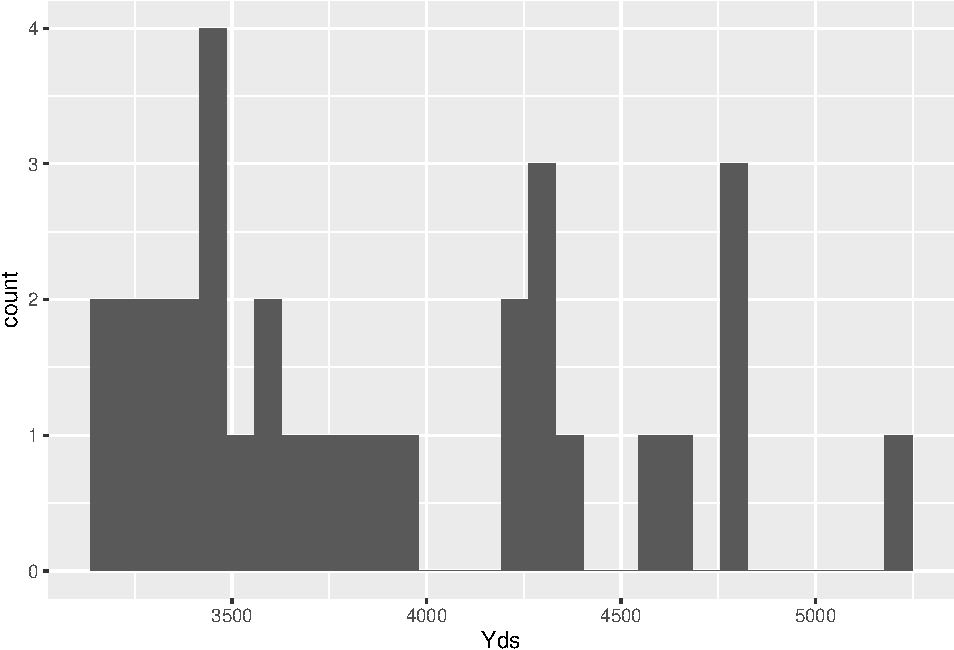
\includegraphics{textbook_files/figure-latex/hist-1.pdf}

Notice how \textbf{\%\textgreater\%} is used to \textbf{pipe} the dataset into ggplot. This is using the pipe function from the \textbf{dplyr} package.

\vfill
\newpage

By default, \textbf{geom\_histogram} uses 30 bins but this is customizable. Let's make the bins have a width of 200.

All good visualizations have good labels. Let's improve the axis labels and give the figure a title.

\begin{Shaded}
\begin{Highlighting}[]
\NormalTok{NFL\_2021\_Team\_Passing }\SpecialCharTok{\%\textgreater{}\%} \FunctionTok{ggplot}\NormalTok{(}\FunctionTok{aes}\NormalTok{(}\AttributeTok{x=}\NormalTok{Yds)) }\SpecialCharTok{+} 
  \FunctionTok{geom\_histogram}\NormalTok{(}\AttributeTok{binwidth =} \DecValTok{200}\NormalTok{) }\SpecialCharTok{+}
  \FunctionTok{labs}\NormalTok{(}\AttributeTok{x=}\StringTok{"Team Passing Yards"}\NormalTok{,}
       \AttributeTok{y=}\StringTok{"Team Passing Touchdowns"}\NormalTok{,}
       \AttributeTok{title=}\StringTok{"NFL Team Passing Yards, 2021"}\NormalTok{)}
\end{Highlighting}
\end{Shaded}

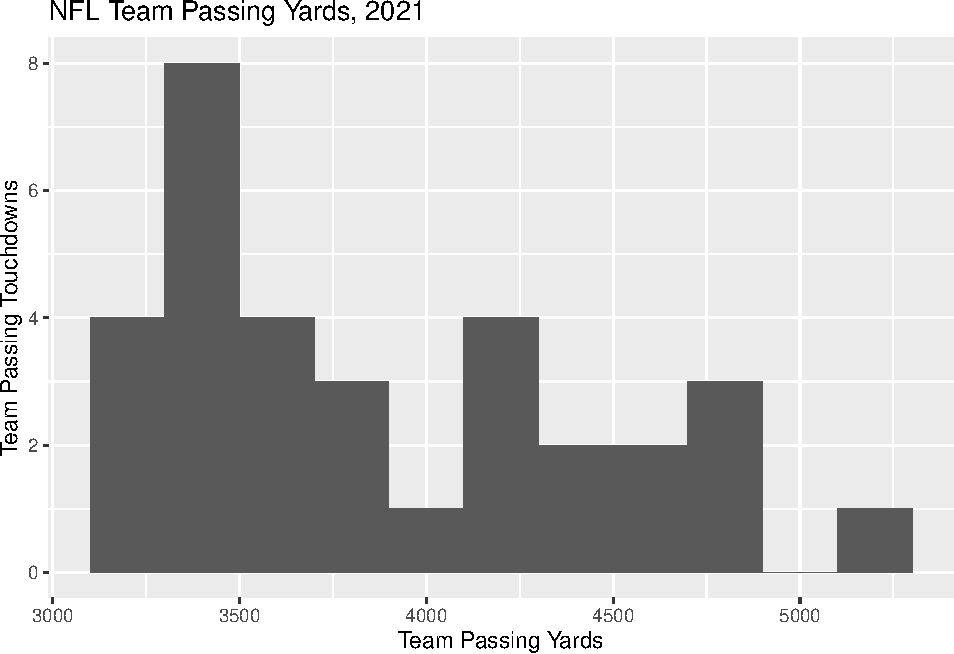
\includegraphics{textbook_files/figure-latex/hist2-1.pdf}

\vfill
\newpage

We also have numerous options to change the appearance of plots when using \textbf{ggplot}. Let's change the bins color to \emph{blue} and change the bin borders to \emph{white}.

\begin{Shaded}
\begin{Highlighting}[]
\NormalTok{NFL\_2021\_Team\_Passing }\SpecialCharTok{\%\textgreater{}\%} \FunctionTok{ggplot}\NormalTok{(}\FunctionTok{aes}\NormalTok{(}\AttributeTok{x=}\NormalTok{Yds)) }\SpecialCharTok{+} 
  \FunctionTok{geom\_histogram}\NormalTok{(}\AttributeTok{color =} \StringTok{"white"}\NormalTok{, }\AttributeTok{fill =} \StringTok{"blue"}\NormalTok{, }\AttributeTok{binwidth =} \DecValTok{200}\NormalTok{) }\SpecialCharTok{+}
  \FunctionTok{labs}\NormalTok{(}\AttributeTok{x=}\StringTok{"Team Passing Yards"}\NormalTok{,}
       \AttributeTok{y=}\StringTok{"Team Passing Touchdowns"}\NormalTok{,}
       \AttributeTok{title=}\StringTok{"NFL Team Passing Yards, 2021"}\NormalTok{)}
\end{Highlighting}
\end{Shaded}

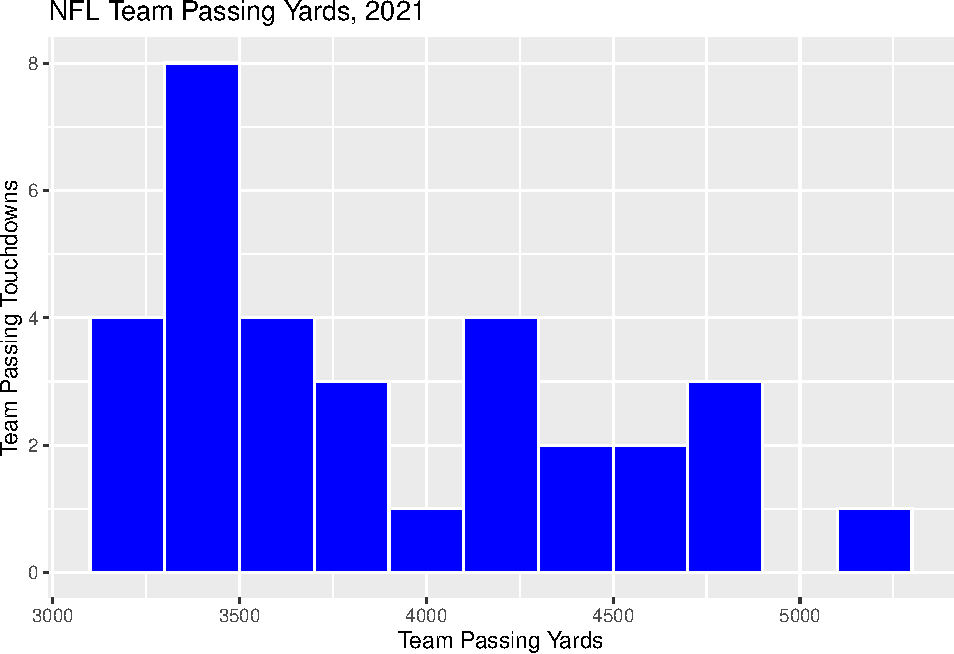
\includegraphics{textbook_files/figure-latex/hist3-1.pdf}
\end{example}

\vfill
\newpage

\hypertarget{bar-plots}{%
\subsection{Bar Plots}\label{bar-plots}}

We can also create bar plots using ggplot using the \textbf{geom\_bar} function.

\begin{example}
Create a bar plot with teams on the horizontal axis and passing touchdowns on the vertical axis.

\begin{Shaded}
\begin{Highlighting}[]
\NormalTok{NFL\_2021\_Team\_Passing }\SpecialCharTok{\%\textgreater{}\%} 
  \FunctionTok{ggplot}\NormalTok{(}\FunctionTok{aes}\NormalTok{(}\AttributeTok{x=}\NormalTok{Tm,}\AttributeTok{y=}\NormalTok{Yds)) }\SpecialCharTok{+}
  \FunctionTok{geom\_bar}\NormalTok{(}\AttributeTok{stat=}\StringTok{"identity"}\NormalTok{)}
\end{Highlighting}
\end{Shaded}

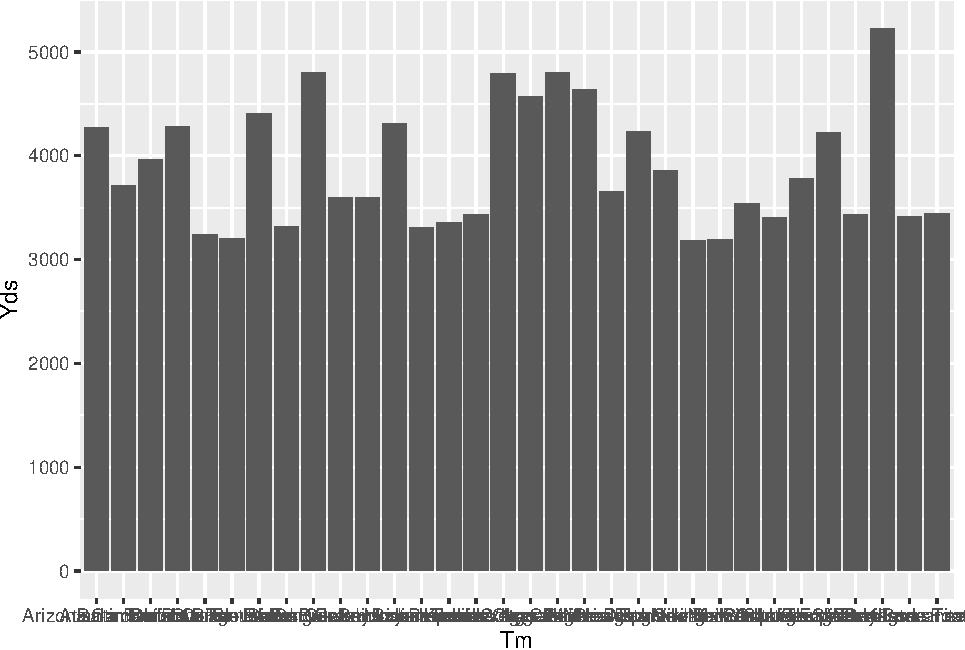
\includegraphics{textbook_files/figure-latex/bar-1.pdf}

\vfill
\newpage

The team labels are a complete mess. Let's fix this and make some adjustments to the axis labels and figure title.

\begin{Shaded}
\begin{Highlighting}[]
\NormalTok{NFL\_2021\_Team\_Passing }\SpecialCharTok{\%\textgreater{}\%} 
  \FunctionTok{ggplot}\NormalTok{(}\FunctionTok{aes}\NormalTok{(}\AttributeTok{x=}\NormalTok{Tm,}\AttributeTok{y=}\NormalTok{Yds)) }\SpecialCharTok{+}
  \FunctionTok{geom\_bar}\NormalTok{(}\AttributeTok{stat=}\StringTok{"identity"}\NormalTok{) }\SpecialCharTok{+} 
  \FunctionTok{labs}\NormalTok{(}\AttributeTok{x=}\StringTok{"Team"}\NormalTok{, }\AttributeTok{y=}\StringTok{"Team Passing Yards"}\NormalTok{, }
       \AttributeTok{title=}\StringTok{"NFL Team Passing Yards, 2021"}\NormalTok{) }\SpecialCharTok{+}
  \FunctionTok{theme}\NormalTok{(}\AttributeTok{axis.text.x =} \FunctionTok{element\_text}\NormalTok{(}\AttributeTok{angle =} \DecValTok{45}\NormalTok{, }\AttributeTok{hjust=}\DecValTok{1}\NormalTok{))}
\end{Highlighting}
\end{Shaded}

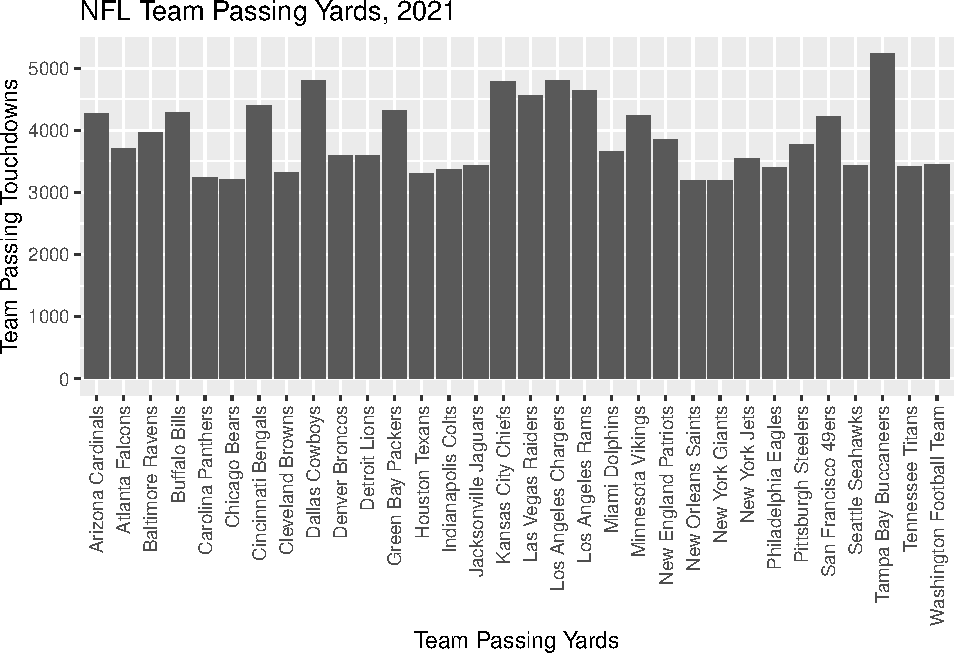
\includegraphics{textbook_files/figure-latex/bar2-1.pdf}

\vfill
\newpage

We can flip this graph if we like as well. Note that when we flip the graph, our labels get in reverse ordering, so this can be fixed using \textbf{fct\_rev()} which is part of the \textbf{forcats} package.

\begin{Shaded}
\begin{Highlighting}[]
\NormalTok{NFL\_2021\_Team\_Passing }\SpecialCharTok{\%\textgreater{}\%} 
  \FunctionTok{ggplot}\NormalTok{(}\FunctionTok{aes}\NormalTok{(}\AttributeTok{x=}\FunctionTok{fct\_rev}\NormalTok{(Tm),}\AttributeTok{y=}\NormalTok{Yds)) }\SpecialCharTok{+}
  \FunctionTok{geom\_bar}\NormalTok{(}\AttributeTok{stat=}\StringTok{"identity"}\NormalTok{) }\SpecialCharTok{+}
  \FunctionTok{labs}\NormalTok{(}\AttributeTok{x=}\StringTok{"Team Passing Yards"}\NormalTok{,}\AttributeTok{y=}\StringTok{"Team"}\NormalTok{,}\AttributeTok{title=}\StringTok{"NFL Team Passing Yards, 2021"}\NormalTok{) }\SpecialCharTok{+}
  \FunctionTok{coord\_flip}\NormalTok{()}
\end{Highlighting}
\end{Shaded}

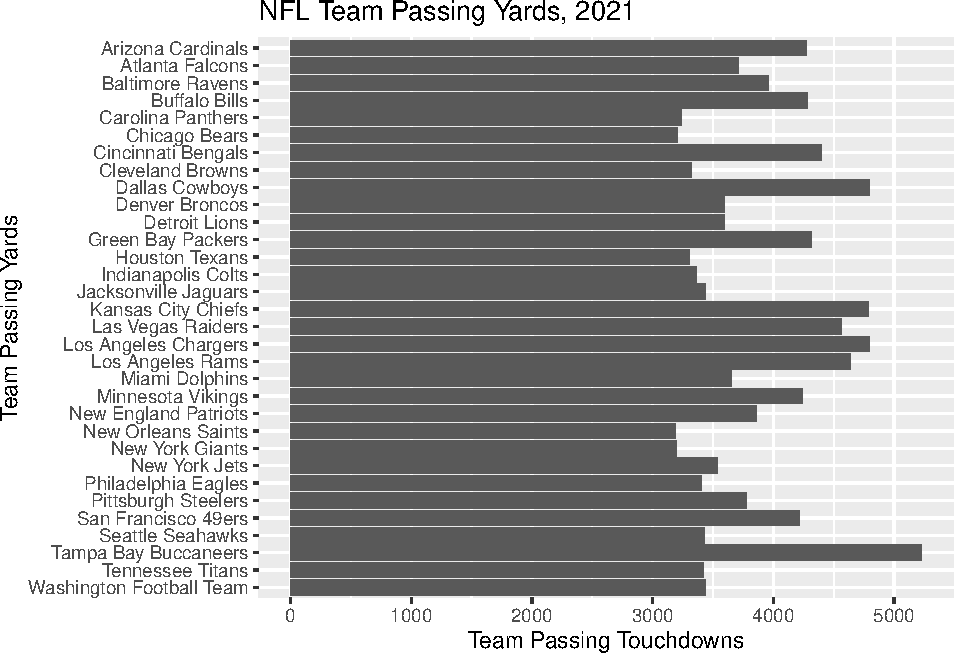
\includegraphics{textbook_files/figure-latex/bar3-1.pdf}
\end{example}

\vfill
\newpage

We can also order the teams from most team passing touchdowns to least using the \texttt{forcats} package.

\begin{Shaded}
\begin{Highlighting}[]
\NormalTok{NFL\_2021\_Team\_Passing }\SpecialCharTok{\%\textgreater{}\%} 
  \FunctionTok{mutate}\NormalTok{(}\AttributeTok{Tm =} \FunctionTok{fct\_reorder}\NormalTok{(Tm,Yds)) }\SpecialCharTok{\%\textgreater{}\%}
  \FunctionTok{ggplot}\NormalTok{(}\FunctionTok{aes}\NormalTok{(}\AttributeTok{x=}\NormalTok{Tm,}\AttributeTok{y=}\NormalTok{Yds)) }\SpecialCharTok{+}
  \FunctionTok{geom\_bar}\NormalTok{(}\AttributeTok{stat=}\StringTok{"identity"}\NormalTok{) }\SpecialCharTok{+}
  \FunctionTok{labs}\NormalTok{(}\AttributeTok{x=}\StringTok{"Team Passing Yards"}\NormalTok{,}
       \AttributeTok{y=}\StringTok{"Team Passing Yards"}\NormalTok{,}
       \AttributeTok{title=}\StringTok{"NFL Team Passing Yards, 2021"}\NormalTok{) }\SpecialCharTok{+}
  \FunctionTok{coord\_flip}\NormalTok{()}
\end{Highlighting}
\end{Shaded}

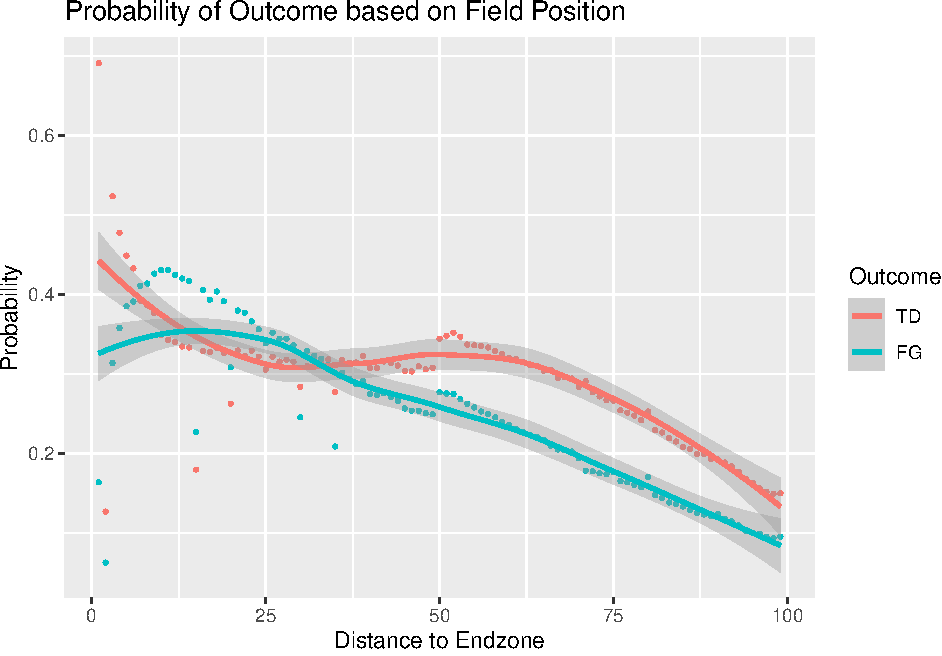
\includegraphics{textbook_files/figure-latex/unnamed-chunk-11-1.pdf}

\vfill
\newpage

\hypertarget{scatter-plots}{%
\subsection{Scatter Plots}\label{scatter-plots}}

Another common and useful visualization is a scatterplot which shows the relationship between two numeric variable. In ggplot, you use \textbf{geom\_point()}.

\begin{example}
Create a scatterplot of Team Passing Yards and Team Passing Touchdowns from the NFL 2021 dataset.

\begin{Shaded}
\begin{Highlighting}[]
\NormalTok{NFL\_2021\_Team\_Passing }\SpecialCharTok{\%\textgreater{}\%}
  \FunctionTok{ggplot}\NormalTok{(}\FunctionTok{aes}\NormalTok{(}\AttributeTok{x=}\NormalTok{Yds,}\AttributeTok{y=}\NormalTok{TD,}\AttributeTok{label=}\NormalTok{Tm)) }\SpecialCharTok{+} 
  \FunctionTok{geom\_point}\NormalTok{() }\SpecialCharTok{+}
  \FunctionTok{labs}\NormalTok{(}\AttributeTok{x=}\StringTok{"Team Passing Yards"}\NormalTok{,}
       \AttributeTok{y=}\StringTok{"Team Passing Touchdowns"}\NormalTok{,}
       \AttributeTok{title=}\StringTok{"NFL Team Passing Yards, 2021"}\NormalTok{)}
\end{Highlighting}
\end{Shaded}

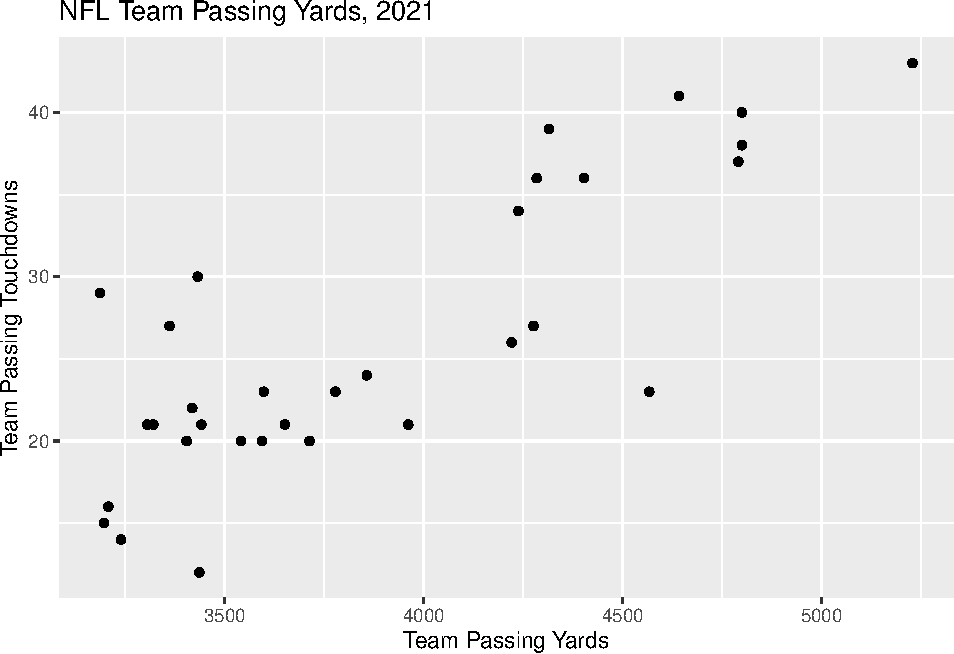
\includegraphics{textbook_files/figure-latex/scatter1-1.pdf}

\vfill
\newpage

We may want to include team labels on this plot, however, it can get messy very quickly with a lot of points.

\begin{Shaded}
\begin{Highlighting}[]
\NormalTok{NFL\_2021\_Team\_Passing }\SpecialCharTok{\%\textgreater{}\%}
  \FunctionTok{ggplot}\NormalTok{(}\FunctionTok{aes}\NormalTok{(}\AttributeTok{x=}\NormalTok{Yds,}\AttributeTok{y=}\NormalTok{TD,}\AttributeTok{label=}\NormalTok{Tm)) }\SpecialCharTok{+} 
  \FunctionTok{geom\_point}\NormalTok{() }\SpecialCharTok{+}
  \FunctionTok{labs}\NormalTok{(}\AttributeTok{x=}\StringTok{"Team Passing Yards"}\NormalTok{,}
       \AttributeTok{y=}\StringTok{"Team Passing Touchdowns"}\NormalTok{,}
       \AttributeTok{title=}\StringTok{"NFL Team Passing Yards, 2021"}\NormalTok{) }\SpecialCharTok{+}
  \FunctionTok{geom\_text}\NormalTok{()}
\end{Highlighting}
\end{Shaded}

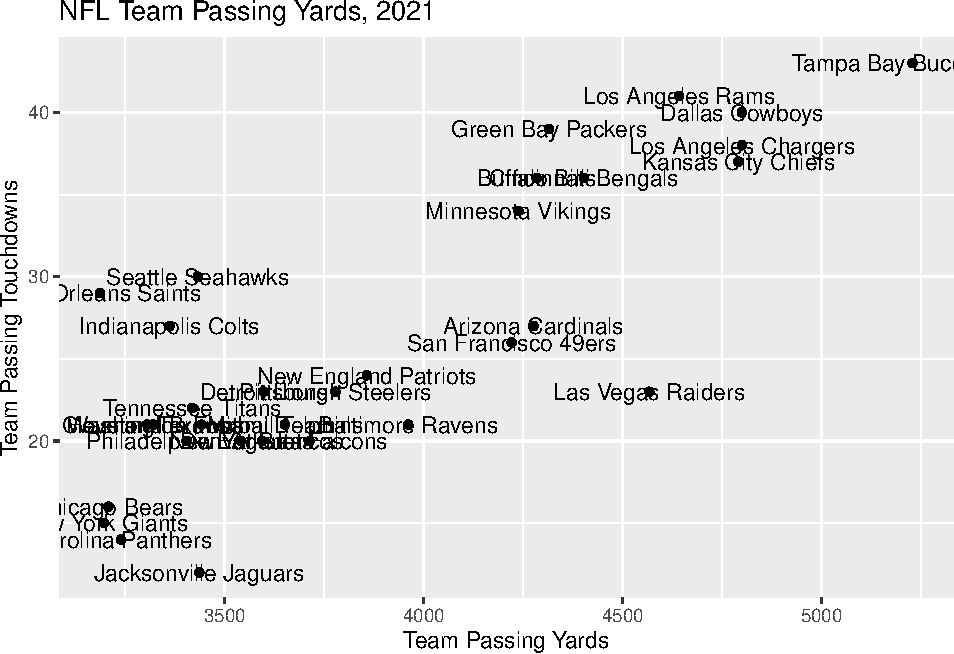
\includegraphics{textbook_files/figure-latex/scatter2-1.pdf}

\vfill
\newpage

Many sports leagues have around 30 teams, so a clean scatterplot with labels can be tricky to make. Here are some options below.

\begin{Shaded}
\begin{Highlighting}[]
\CommentTok{\# install ggrepel package}
\FunctionTok{library}\NormalTok{(ggrepel)}
\NormalTok{NFL\_2021\_Team\_Passing }\SpecialCharTok{\%\textgreater{}\%}
  \FunctionTok{ggplot}\NormalTok{(}\FunctionTok{aes}\NormalTok{(}\AttributeTok{x=}\NormalTok{Yds,}\AttributeTok{y=}\NormalTok{TD,}\AttributeTok{label=}\NormalTok{Tm)) }\SpecialCharTok{+} 
  \FunctionTok{geom\_point}\NormalTok{() }\SpecialCharTok{+}
  \FunctionTok{labs}\NormalTok{(}\AttributeTok{x=}\StringTok{"Team Passing Yards"}\NormalTok{,}
       \AttributeTok{y=}\StringTok{"Team Passing Touchdowns"}\NormalTok{,}
       \AttributeTok{title=}\StringTok{"NFL Team Passing Yards, 2021"}\NormalTok{) }\SpecialCharTok{+}
  \FunctionTok{geom\_text\_repel}\NormalTok{()}
\end{Highlighting}
\end{Shaded}

\begin{verbatim}
## Warning: ggrepel: 9 unlabeled data points (too many overlaps). Consider
## increasing max.overlaps
\end{verbatim}

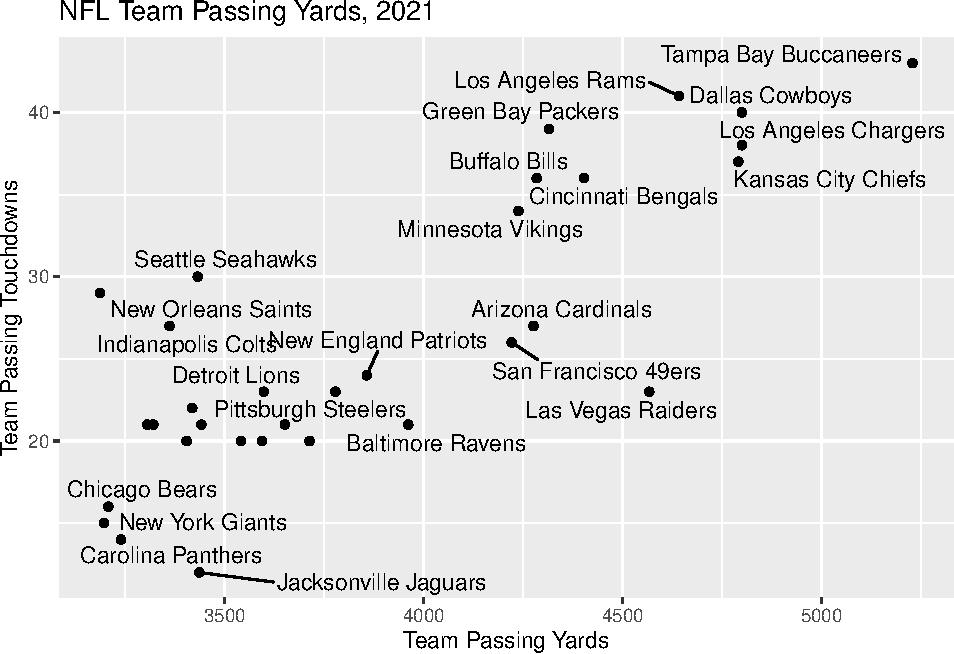
\includegraphics{textbook_files/figure-latex/scatter3-1.pdf}

\newpage

\begin{Shaded}
\begin{Highlighting}[]
\NormalTok{NFL\_2021\_Team\_Passing}\SpecialCharTok{$}\NormalTok{Abbr }\OtherTok{\textless{}{-}} 
  \FunctionTok{c}\NormalTok{(}\StringTok{"TB"}\NormalTok{,}\StringTok{"LAC"}\NormalTok{,}\StringTok{"DAL"}\NormalTok{,}\StringTok{"KC"}\NormalTok{,}\StringTok{"LAR"}\NormalTok{,}\StringTok{"LV"}\NormalTok{,}\StringTok{"CIN"}\NormalTok{,}\StringTok{"GB"}\NormalTok{,}\StringTok{"BUF"}\NormalTok{,}\StringTok{"ARI"}\NormalTok{,}\StringTok{"MIN"}\NormalTok{,}\StringTok{"SF"}\NormalTok{,}
    \StringTok{"BAL"}\NormalTok{,}\StringTok{"NE"}\NormalTok{,}\StringTok{"PIT"}\NormalTok{,}\StringTok{"ATL"}\NormalTok{,}\StringTok{"MIA"}\NormalTok{,}\StringTok{"DET"}\NormalTok{,}\StringTok{"DEN"}\NormalTok{,}\StringTok{"NYJ"}\NormalTok{,}\StringTok{"WAS"}\NormalTok{,}\StringTok{"JAC"}\NormalTok{,}\StringTok{"SEA"}\NormalTok{,}
    \StringTok{"TEN"}\NormalTok{,}\StringTok{"PHI"}\NormalTok{,}\StringTok{"IND"}\NormalTok{,}\StringTok{"CLE"}\NormalTok{,}\StringTok{"HOU"}\NormalTok{,}\StringTok{"CAR"}\NormalTok{,}\StringTok{"CHI"}\NormalTok{,}\StringTok{"NYG"}\NormalTok{,}\StringTok{"NO"}\NormalTok{)}

\NormalTok{NFL\_2021\_Team\_Passing }\SpecialCharTok{\%\textgreater{}\%}
  \FunctionTok{ggplot}\NormalTok{(}\FunctionTok{aes}\NormalTok{(}\AttributeTok{x=}\NormalTok{Yds,}\AttributeTok{y=}\NormalTok{TD,}\AttributeTok{label=}\NormalTok{Abbr)) }\SpecialCharTok{+} 
  \FunctionTok{geom\_point}\NormalTok{() }\SpecialCharTok{+}
  \FunctionTok{scale\_x\_continuous}\NormalTok{(}\AttributeTok{limits=}\FunctionTok{c}\NormalTok{(}\DecValTok{2750}\NormalTok{,}\DecValTok{5250}\NormalTok{)) }\SpecialCharTok{+}
  \FunctionTok{labs}\NormalTok{(}\AttributeTok{x=}\StringTok{"Team Passing Yards"}\NormalTok{,}\AttributeTok{y=}\StringTok{"Team Passing Touchdowns"}\NormalTok{,}
       \AttributeTok{title=}\StringTok{"NFL Team Passing Yards, 2021"}\NormalTok{) }\SpecialCharTok{+}
  \FunctionTok{geom\_text\_repel}\NormalTok{(}\AttributeTok{box.padding =} \FloatTok{0.2}\NormalTok{) }
\end{Highlighting}
\end{Shaded}

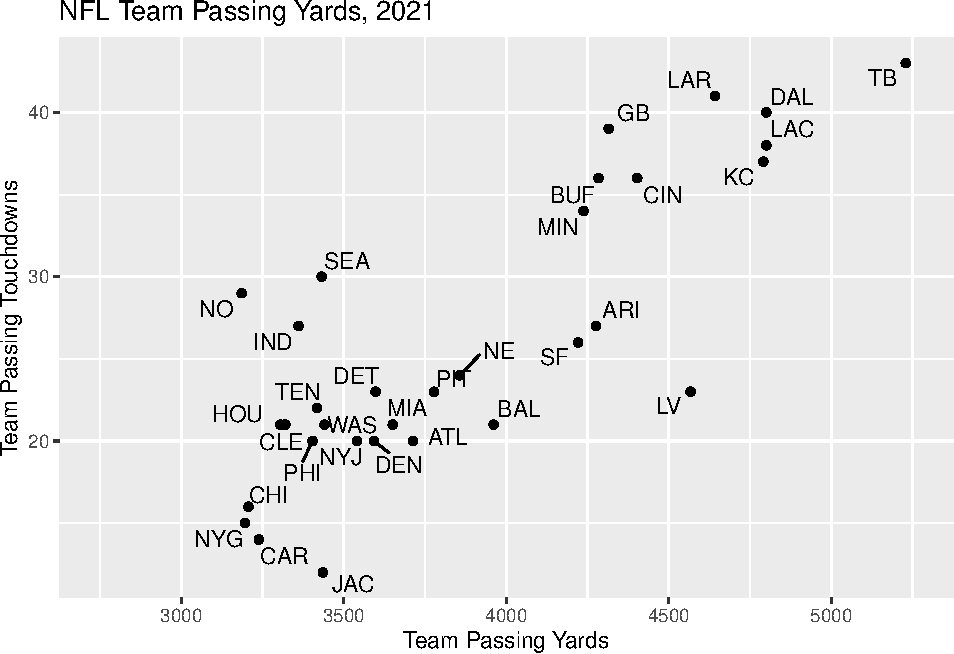
\includegraphics{textbook_files/figure-latex/scatter4-1.pdf}
\end{example}

\newpage

\begin{Shaded}
\begin{Highlighting}[]
\CommentTok{\# install.packages("nflplotR")}
\FunctionTok{library}\NormalTok{(nflplotR)}

\NormalTok{NFL\_2021\_Team\_Passing }\SpecialCharTok{\%\textgreater{}\%}
  \FunctionTok{ggplot}\NormalTok{(}\FunctionTok{aes}\NormalTok{(}\AttributeTok{x=}\NormalTok{Yds,}\AttributeTok{y=}\NormalTok{TD)) }\SpecialCharTok{+}
  \FunctionTok{scale\_x\_continuous}\NormalTok{(}\AttributeTok{limits=}\FunctionTok{c}\NormalTok{(}\DecValTok{2750}\NormalTok{,}\DecValTok{5250}\NormalTok{)) }\SpecialCharTok{+}
\NormalTok{  nflplotR}\SpecialCharTok{::}\FunctionTok{geom\_nfl\_logos}\NormalTok{(}\FunctionTok{aes}\NormalTok{(}\AttributeTok{team\_abbr =}\NormalTok{ Abbr), }\AttributeTok{width =} \FloatTok{0.04}\NormalTok{, }\AttributeTok{alpha =} \FloatTok{0.7}\NormalTok{) }\SpecialCharTok{+}
  \FunctionTok{labs}\NormalTok{(}\AttributeTok{x=}\StringTok{"Team Passing Yards"}\NormalTok{,}\AttributeTok{y=}\StringTok{"Team Passing Touchdowns"}\NormalTok{,}
       \AttributeTok{title=}\StringTok{"NFL Team Passing Yards, 2021"}\NormalTok{)}
\end{Highlighting}
\end{Shaded}

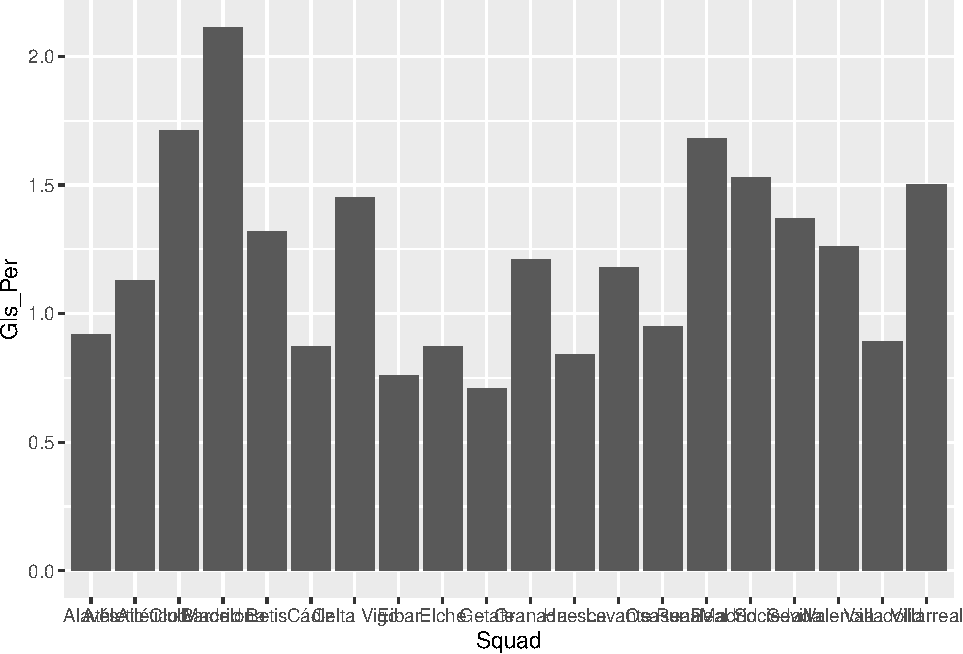
\includegraphics{textbook_files/figure-latex/unnamed-chunk-12-1.pdf}

\newpage

\hypertarget{kable-tables}{%
\subsection{Kable Tables}\label{kable-tables}}

We can build nice tables using \texttt{kableR} and \texttt{kableExtra}. Let's look at a few options.

\begin{Shaded}
\begin{Highlighting}[]
\CommentTok{\# Use a smaller dataset as an example}
\NormalTok{NFL21 }\OtherTok{\textless{}{-}}\NormalTok{ NFL\_2021\_Team\_Passing }\SpecialCharTok{\%\textgreater{}\%} \FunctionTok{select}\NormalTok{(}\DecValTok{2}\SpecialCharTok{:}\DecValTok{8}\NormalTok{) }\SpecialCharTok{\%\textgreater{}\%} \FunctionTok{slice\_head}\NormalTok{(}\AttributeTok{n =} \DecValTok{5}\NormalTok{)}

\CommentTok{\# Default output for tabular data}
\NormalTok{NFL21}
\end{Highlighting}
\end{Shaded}

\begin{verbatim}
## # A tibble: 5 x 7
##   Tm                       G   Cmp   Att `Cmp%`   Yds    TD
##   <chr>                <dbl> <dbl> <dbl>  <dbl> <dbl> <dbl>
## 1 Tampa Bay Buccaneers    17   492   731   67.3  5229    43
## 2 Los Angeles Chargers    17   443   674   65.7  4800    38
## 3 Dallas Cowboys          17   444   647   68.6  4800    40
## 4 Kansas City Chiefs      17   448   675   66.4  4791    37
## 5 Los Angeles Rams        17   406   607   66.9  4642    41
\end{verbatim}

You can find additional details on customizing kable tables at ~\url{https://cran.r-project.org/web/packages/kableExtra/vignettes/awesome_table_in_pdf.pdf}

\begin{Shaded}
\begin{Highlighting}[]
\CommentTok{\# Output using Kable (with no additional options)}
\FunctionTok{library}\NormalTok{(kableExtra)}

\CommentTok{\# Output using Kable and Kable{-}Styling and some additional options}
\NormalTok{NFL21 }\SpecialCharTok{\%\textgreater{}\%} \FunctionTok{kable}\NormalTok{() }\SpecialCharTok{\%\textgreater{}\%} \FunctionTok{kable\_styling}\NormalTok{(}\AttributeTok{latex\_options=}\StringTok{"hold\_position"}\NormalTok{)}
\end{Highlighting}
\end{Shaded}

\begin{table}[!h]
\centering
\begin{tabular}{l|r|r|r|r|r|r}
\hline
Tm & G & Cmp & Att & Cmp\% & Yds & TD\\
\hline
Tampa Bay Buccaneers & 17 & 492 & 731 & 67.3 & 5229 & 43\\
\hline
Los Angeles Chargers & 17 & 443 & 674 & 65.7 & 4800 & 38\\
\hline
Dallas Cowboys & 17 & 444 & 647 & 68.6 & 4800 & 40\\
\hline
Kansas City Chiefs & 17 & 448 & 675 & 66.4 & 4791 & 37\\
\hline
Los Angeles Rams & 17 & 406 & 607 & 66.9 & 4642 & 41\\
\hline
\end{tabular}
\end{table}

\begin{Shaded}
\begin{Highlighting}[]
\CommentTok{\# More options}
\NormalTok{NFL21 }\SpecialCharTok{\%\textgreater{}\%} \FunctionTok{kable}\NormalTok{(}\AttributeTok{booktabs=}\ConstantTok{TRUE}\NormalTok{) }\SpecialCharTok{\%\textgreater{}\%} \FunctionTok{kable\_styling}\NormalTok{(}\AttributeTok{latex\_options=}\StringTok{"hold\_position"}\NormalTok{)}
\end{Highlighting}
\end{Shaded}

\begin{table}[!h]
\centering
\begin{tabular}{lrrrrrr}
\toprule
Tm & G & Cmp & Att & Cmp\% & Yds & TD\\
\midrule
Tampa Bay Buccaneers & 17 & 492 & 731 & 67.3 & 5229 & 43\\
Los Angeles Chargers & 17 & 443 & 674 & 65.7 & 4800 & 38\\
Dallas Cowboys & 17 & 444 & 647 & 68.6 & 4800 & 40\\
Kansas City Chiefs & 17 & 448 & 675 & 66.4 & 4791 & 37\\
Los Angeles Rams & 17 & 406 & 607 & 66.9 & 4642 & 41\\
\bottomrule
\end{tabular}
\end{table}

\vfill
\newpage

If you are going to use kable tables frequently in a document, you can write a short function to set your default options. After I ran the function below, the function \emph{kt} will produce a kable table with my options set.

\begin{Shaded}
\begin{Highlighting}[]
\CommentTok{\# kable table global setup}
\NormalTok{kt }\OtherTok{\textless{}{-}} \ControlFlowTok{function}\NormalTok{(data) \{}
\NormalTok{  knitr}\SpecialCharTok{::}\FunctionTok{kable}\NormalTok{(data, }\AttributeTok{digits=}\DecValTok{3}\NormalTok{,}\AttributeTok{linesep=}\StringTok{\textquotesingle{}\textquotesingle{}}\NormalTok{,}\AttributeTok{booktabs=}\ConstantTok{TRUE}\NormalTok{) }\SpecialCharTok{\%\textgreater{}\%} \FunctionTok{kable\_styling}\NormalTok{(}\AttributeTok{latex\_options=}\StringTok{\textquotesingle{}HOLD\_position\textquotesingle{}}\NormalTok{, }\AttributeTok{full\_width =}\NormalTok{ F, }\AttributeTok{position =} \StringTok{"center"}\NormalTok{)}
\NormalTok{\}}
\end{Highlighting}
\end{Shaded}

\begin{Shaded}
\begin{Highlighting}[]
\NormalTok{NFL21 }\SpecialCharTok{\%\textgreater{}\%} \FunctionTok{kt}\NormalTok{()}
\end{Highlighting}
\end{Shaded}

\begin{table}[H]
\centering
\begin{tabular}{lrrrrrr}
\toprule
Tm & G & Cmp & Att & Cmp\% & Yds & TD\\
\midrule
Tampa Bay Buccaneers & 17 & 492 & 731 & 67.3 & 5229 & 43\\
Los Angeles Chargers & 17 & 443 & 674 & 65.7 & 4800 & 38\\
Dallas Cowboys & 17 & 444 & 647 & 68.6 & 4800 & 40\\
Kansas City Chiefs & 17 & 448 & 675 & 66.4 & 4791 & 37\\
Los Angeles Rams & 17 & 406 & 607 & 66.9 & 4642 & 41\\
\bottomrule
\end{tabular}
\end{table}

\newpage

\hypertarget{baseball}{%
\section{Baseball}\label{baseball}}

Baseball rules YouTube video: \url{https://www.youtube.com/watch?v=skOsApsF0jQ\&t=63s}

\hypertarget{hitting-statistics}{%
\subsection{Hitting Statistics}\label{hitting-statistics}}

\hypertarget{basic-hitting-statistics}{%
\subsubsection{Basic Hitting Statistics}\label{basic-hitting-statistics}}

\begin{itemize}
\item
  \textbf{Plate Appearances} (PA): number of completed batting appearances
\item
  \textbf{At-Bats} (AB): Batting appearances, not including bases on balls, hit by pitch, sacrifices, interference, or obstruction
\item
  \textbf{Hits} (H): Times reached base because of a batted, fair ball without error by the defense
\item
  \textbf{Singles} (1B): Hits on which the batter reached first base safely without the contribution of a fielding error
\item
  \textbf{Doubles} (2B): Hits on which the batter reached second base safely without the contribution of a fielding error
\item
  \textbf{Triples} (3B): Hits on which the batter reached third base safely without the contribution of a fielding error
\item
  \textbf{Home Runs} (HR): Hits on which the batter successfully touched all four bases, without the contribution of a fielding error
\item
  \textbf{Total Bases} (TB): One for each single, two for each double, three for each triple, and four for each home run
\item
  \textbf{Hit by Pitch} (HBP): Times touched by a pitch and awarded first base as a result
\item
  \textbf{Sacrifice Fly} (SF): Number of fly ball outs which allow another runner to advance on the basepaths or score
\item
  \textbf{Base on Balls} (BB or Walk): Times receiving four balls and advancing to first base
\item
  \textbf{Intentional Base on Balls} (IBB or Intentional Walk): Times receiving four balls \emph{intentionally} and advancing to first base
\item
  \textbf{Strikeout} (K): Number of times that strike three is taken or swung at and missed, or bunted foul
\item
  \textbf{Runs} (R): Times reached home base legally and safely
\item
  \textbf{Runs Batted In} (RBI): Number of runners who scored due to a batters's action, except when batter grounded into double play or reached on an error
\item
  \textbf{Batting Average} (AVG or BA): Hits divided by at bats
\item
  \textbf{On Base Percentage/Average} (OBP or OBA): Times reached base (H + BB + HBP) divided by at bats plus walks plus hit by pitch plus sacrifice flies (AB + BB + HBP + SF)
\item
  \textbf{Slugging Percentage/Average} (SLG): Total bases divided by at-bats
\item
  \textbf{On-base Plus Slugging} (OPS): On-base percentage plus slugging average
\end{itemize}

\newpage

\hypertarget{advanced-baseball-hitting-statistics}{%
\subsubsection{Advanced Baseball Hitting Statistics}\label{advanced-baseball-hitting-statistics}}

\begin{itemize}
\item
  \textbf{Isolated Power} (ISO): Slugging percentage minus Batting average
\item
  \textbf{On-base Plus Slugging Plus} (OPS+): OPS normalized for park effects with 100 being league average
\item
  \textbf{Weighted On-Base Average} (wOBA): Hitting rate statistic that attempts to credit the hitter for the value of each outcome. The following formula can be updated each year based on the scoring environment. The following formula was updated for the 2021 season.
\end{itemize}

\[wOBA = \frac{0.69 \cdot (BB - IBB) + 0.719 \cdot HBP + 0.87 \cdot 1B + 1.217 \cdot 2B + 1.529 \cdot 3B + 1.94 \cdot HR}{AB + BB - IBB + SF + HBP}\]

\begin{itemize}
\tightlist
\item
  \textbf{Expected Weighted On-Base Average} (xwOBA): Hitting rate statistic that attempts to credit the hitter for the value of each \emph{expected} outcome based on Statcast data.
\end{itemize}

\hypertarget{pitching-statistics}{%
\subsection{Pitching Statistics}\label{pitching-statistics}}

\hypertarget{basic-pitching-statistics}{%
\subsubsection{Basic Pitching Statistics}\label{basic-pitching-statistics}}

\begin{itemize}
\item
  \textbf{Innings Pitched} (IP): Number of outs recorded while pitching divided by three
\item
  \textbf{Strikeout} (K): Number of batters who received strike three
\item
  \textbf{Base on Balls} (BB or Walk): Times pitching four balls, allowing the batter-runner to advance to first base
\item
  \textbf{Hits Allowed} (H): Total hits allowed
\item
  \textbf{Wins} (W): Number of games where pitcher was pitching while his team took the lead and went on to win
\item
  \textbf{Losses} (L): Number of games where pitcher was pitching while the opposing team took the lead, never lost the lead, and went on to win
\item
  \textbf{Earned Runs} (ER): Number of runs that did not occur as a result of errors or passed balls
\item
  \textbf{Earned Run Average} (ERA): Earned runs times innings in a game (usually nine) divided by innings pitched
\item
  \textbf{Walks and Hits Per Inning Pitched} (WHIP): Walks plus hits allowed divided by innings pitched
\end{itemize}

\hypertarget{advanced-pitching-statistics}{%
\subsubsection{Advanced Pitching Statistics}\label{advanced-pitching-statistics}}

\begin{itemize}
\tightlist
\item
  \textbf{Fielding Independent Pitching} (FIP): Statistic that estimates a pitcher's run prevention independent of the performance of the defense
\end{itemize}

\[FIP = \frac{13 \cdot HR + 3 \cdot (BB + HBP) - 2 \cdot K}{IP} + FIP_{constant}\]

The \(FIP_{constant}\) is generally around 3.10 and is put FIP on a scale similar to ERA.

\begin{itemize}
\tightlist
\item
  \textbf{Expected Fielding Independent Pitching} (xFIP): Statistic that estimates a pitcher's expected run prevention independent of the performance of the defense
\end{itemize}

\[xFIP = \frac{13 \cdot (Fly Balls \cdot LgHR/FB\%)+3 \cdot (BB + HBP) - 2 \cdot K}{IP} + FIP_{constant}\]

\hypertarget{wins-above-replacement}{%
\subsection{Wins Above Replacement}\label{wins-above-replacement}}

\begin{itemize}
\tightlist
\item
  \textbf{Wins Above Replacement} (WAR): Estimated number of wins that a player has outperformed a replacement player by with the same playing time. This is one of the most crucial statistics in Sabermetrics.
\end{itemize}

More about WAR from Fangraphs: \url{https://library.fangraphs.com/misc/war/}

\emph{References:}\\
\url{https://www.baseball-reference.com/bullpen/Baseball_statistics}\strut \\
\url{https://blogs.fangraphs.com/glossary/}\strut \\
\url{https://library.fangraphs.com/fangraphs-library-glossary/}\strut \\

\newpage

\hypertarget{calculating-hitting-statistics}{%
\subsection{Calculating Hitting Statistics}\label{calculating-hitting-statistics}}

\begin{example}
Using the Colorado Rockies 2021 individual hitting statistics, calculate the AVG, OBA, SLG, OPS, ISO, wOBA.
\end{example}

\begin{Shaded}
\begin{Highlighting}[]
\CommentTok{\# load data file and look at the header}
\NormalTok{rox21 }\OtherTok{\textless{}{-}} \FunctionTok{read\_csv}\NormalTok{(}\StringTok{"data/rockies\_hitting2021.csv"}\NormalTok{)}
\NormalTok{rox21 }\SpecialCharTok{\%\textgreater{}\%} \FunctionTok{slice\_head}\NormalTok{(}\AttributeTok{n=}\DecValTok{5}\NormalTok{) }\SpecialCharTok{\%\textgreater{}\%} \FunctionTok{kt}\NormalTok{()}
\end{Highlighting}
\end{Shaded}

\begin{table}[H]
\centering
\begin{tabular}{lrrrrrrrrrrrrrr}
\toprule
Name & PA & AB & R & H & 2B & 3B & HR & RBI & BB & IBB & SO & HBP & SF & oWAR\\
\midrule
Elias Diaz & 371 & 338 & 52 & 83 & 18 & 1 & 18 & 44 & 30 & 1 & 60 & 2 & 1 & 1.1\\
C.J. Cron & 547 & 470 & 70 & 132 & 31 & 1 & 28 & 92 & 60 & 3 & 117 & 13 & 4 & 3.1\\
Brendan Rodgers & 415 & 387 & 49 & 110 & 21 & 3 & 15 & 51 & 19 & 0 & 84 & 7 & 2 & 1.9\\
Trevor Story & 595 & 526 & 88 & 132 & 34 & 5 & 24 & 75 & 53 & 2 & 139 & 11 & 5 & 3.4\\
Ryan McMahon* & 596 & 528 & 80 & 134 & 32 & 1 & 23 & 86 & 59 & 2 & 147 & 4 & 5 & 1.7\\
\bottomrule
\end{tabular}
\end{table}

\begin{Shaded}
\begin{Highlighting}[]
\CommentTok{\# Create new variables using the mutate function}
\NormalTok{rox21 }\OtherTok{\textless{}{-}}\NormalTok{ rox21 }\SpecialCharTok{\%\textgreater{}\%} 
  \FunctionTok{mutate}\NormalTok{(}\AttributeTok{AVG =}\NormalTok{ H}\SpecialCharTok{/}\NormalTok{AB,}\DecValTok{3}\NormalTok{) }\SpecialCharTok{\%\textgreater{}\%}
  \FunctionTok{mutate}\NormalTok{(}\AttributeTok{OBA =}\NormalTok{ (H }\SpecialCharTok{+}\NormalTok{ BB }\SpecialCharTok{+}\NormalTok{ HBP)}\SpecialCharTok{/}\NormalTok{(AB }\SpecialCharTok{+}\NormalTok{ BB }\SpecialCharTok{+}\NormalTok{ HBP }\SpecialCharTok{+}\NormalTok{ SF)) }\SpecialCharTok{\%\textgreater{}\%}
  \FunctionTok{mutate}\NormalTok{(}\AttributeTok{SLG =}\NormalTok{ ((H}\SpecialCharTok{{-}}\StringTok{\textasciigrave{}}\AttributeTok{2B}\StringTok{\textasciigrave{}}\SpecialCharTok{{-}}\StringTok{\textasciigrave{}}\AttributeTok{3B}\StringTok{\textasciigrave{}}\SpecialCharTok{{-}}\NormalTok{HR) }\SpecialCharTok{+} \DecValTok{2}\SpecialCharTok{*}\StringTok{\textasciigrave{}}\AttributeTok{2B}\StringTok{\textasciigrave{}} \SpecialCharTok{+} \DecValTok{3}\SpecialCharTok{*}\StringTok{\textasciigrave{}}\AttributeTok{3B}\StringTok{\textasciigrave{}} \SpecialCharTok{+} \DecValTok{4}\SpecialCharTok{*}\NormalTok{HR)}\SpecialCharTok{/}\NormalTok{AB) }\SpecialCharTok{\%\textgreater{}\%}
  \FunctionTok{mutate}\NormalTok{(}\AttributeTok{OPS =}\NormalTok{ SLG }\SpecialCharTok{+}\NormalTok{ OBA) }\SpecialCharTok{\%\textgreater{}\%}
  \FunctionTok{mutate}\NormalTok{(}\AttributeTok{wOBA =}\NormalTok{ (}\FloatTok{0.692} \SpecialCharTok{*}\NormalTok{ (BB }\SpecialCharTok{{-}}\NormalTok{ IBB) }\SpecialCharTok{+} \FloatTok{0.722} \SpecialCharTok{*}\NormalTok{ HBP }\SpecialCharTok{+} \FloatTok{0.879} \SpecialCharTok{*}\NormalTok{ (H}\SpecialCharTok{{-}}\StringTok{\textasciigrave{}}\AttributeTok{2B}\StringTok{\textasciigrave{}}\SpecialCharTok{{-}}\StringTok{\textasciigrave{}}\AttributeTok{3B}\StringTok{\textasciigrave{}}\SpecialCharTok{{-}}\NormalTok{HR) }\SpecialCharTok{+} \FloatTok{1.242} \SpecialCharTok{*} \StringTok{\textasciigrave{}}\AttributeTok{2B}\StringTok{\textasciigrave{}} \SpecialCharTok{+} \FloatTok{1.568} \SpecialCharTok{*} \StringTok{\textasciigrave{}}\AttributeTok{3B}\StringTok{\textasciigrave{}} \SpecialCharTok{+} \FloatTok{2.007} \SpecialCharTok{*}\NormalTok{ HR)}\SpecialCharTok{/}\NormalTok{(AB }\SpecialCharTok{+}\NormalTok{ BB }\SpecialCharTok{{-}}\NormalTok{ IBB }\SpecialCharTok{+}\NormalTok{ SF }\SpecialCharTok{+}\NormalTok{ HBP)) }\SpecialCharTok{\%\textgreater{}\%}
  \FunctionTok{mutate}\NormalTok{(}\AttributeTok{ISO =}\NormalTok{ SLG}\SpecialCharTok{{-}}\NormalTok{AVG)}
\NormalTok{rox21 }\SpecialCharTok{\%\textgreater{}\%} \FunctionTok{slice\_head}\NormalTok{(}\AttributeTok{n=}\DecValTok{5}\NormalTok{) }\SpecialCharTok{\%\textgreater{}\%} \FunctionTok{select}\NormalTok{(Name,PA,AVG,OBA,SLG,OPS,wOBA,ISO) }\SpecialCharTok{\%\textgreater{}\%} \FunctionTok{kt}\NormalTok{()}
\end{Highlighting}
\end{Shaded}

\begin{table}[H]
\centering
\begin{tabular}{lrrrrrrr}
\toprule
Name & PA & AVG & OBA & SLG & OPS & wOBA & ISO\\
\midrule
Elias Diaz & 371 & 0.246 & 0.310 & 0.464 & 0.774 & 0.330 & 0.219\\
C.J. Cron & 547 & 0.281 & 0.375 & 0.530 & 0.905 & 0.383 & 0.249\\
Brendan Rodgers & 415 & 0.284 & 0.328 & 0.470 & 0.798 & 0.341 & 0.186\\
Trevor Story & 595 & 0.251 & 0.329 & 0.471 & 0.801 & 0.341 & 0.221\\
Ryan McMahon* & 596 & 0.254 & 0.331 & 0.449 & 0.779 & 0.334 & 0.195\\
\bottomrule
\end{tabular}
\end{table}

\vfill
\newpage

\begin{example}
oWAR is Baseball Reference's offensive WAR statistic. Note that Baseball Reference and Fangraphs use different formulas when calculating WAR though their results are typically similar. For Rockies players with at least 100 at-bats in 2021, what hitting statistics are most and least correlated to oWAR?
\end{example}

\begin{Shaded}
\begin{Highlighting}[]
\CommentTok{\# Let\textquotesingle{}s remove players with less than 100 ABs}
\NormalTok{rox21\_100 }\OtherTok{\textless{}{-}}\NormalTok{ rox21 }\SpecialCharTok{\%\textgreater{}\%} \FunctionTok{filter}\NormalTok{(AB }\SpecialCharTok{\textgreater{}=} \DecValTok{100}\NormalTok{)}

\CommentTok{\# GGally package has a nice pairs plotting function}
\FunctionTok{library}\NormalTok{(}\StringTok{"GGally"}\NormalTok{)}

\CommentTok{\# Standard hitting statistics}
\NormalTok{rox21\_100 }\SpecialCharTok{\%\textgreater{}\%} \FunctionTok{select}\NormalTok{(oWAR,H,}\StringTok{\textasciigrave{}}\AttributeTok{2B}\StringTok{\textasciigrave{}}\NormalTok{,}\StringTok{\textasciigrave{}}\AttributeTok{3B}\StringTok{\textasciigrave{}}\NormalTok{,HR,R,RBI) }\SpecialCharTok{\%\textgreater{}\%} \FunctionTok{ggpairs}\NormalTok{() }\SpecialCharTok{+}
  \FunctionTok{theme}\NormalTok{(}\AttributeTok{axis.text.x =} \FunctionTok{element\_text}\NormalTok{(}\AttributeTok{angle =} \DecValTok{45}\NormalTok{, }\AttributeTok{hjust =} \DecValTok{1}\NormalTok{))}
\end{Highlighting}
\end{Shaded}

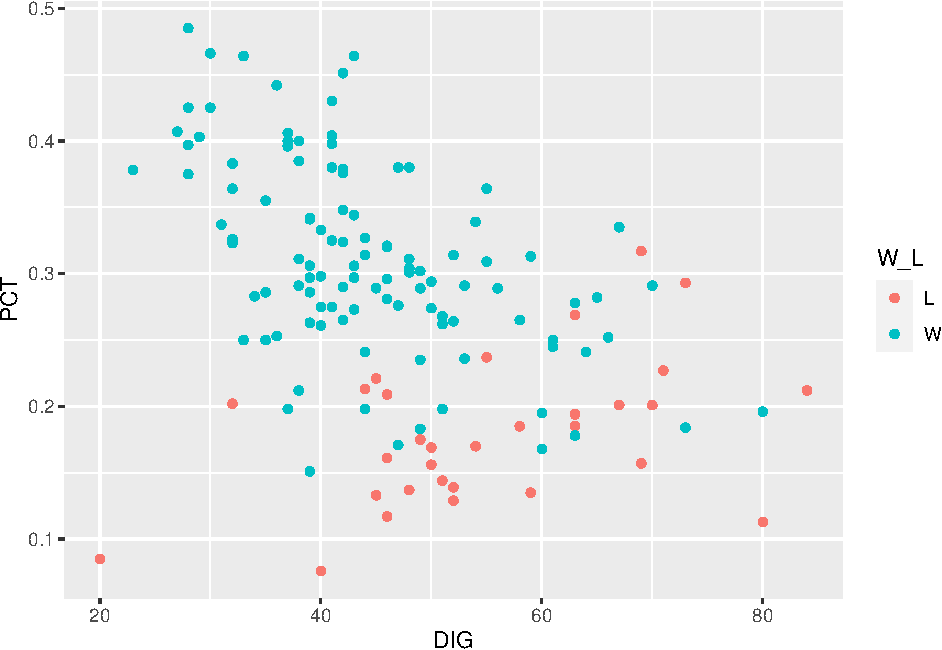
\includegraphics{textbook_files/figure-latex/unnamed-chunk-19-1.pdf}

\begin{Shaded}
\begin{Highlighting}[]
\CommentTok{\# Rate statistics}
\NormalTok{rox21\_100 }\SpecialCharTok{\%\textgreater{}\%} \FunctionTok{select}\NormalTok{(oWAR,AVG,OBA,SLG,OPS,wOBA) }\SpecialCharTok{\%\textgreater{}\%} \FunctionTok{ggpairs}\NormalTok{()}
\end{Highlighting}
\end{Shaded}

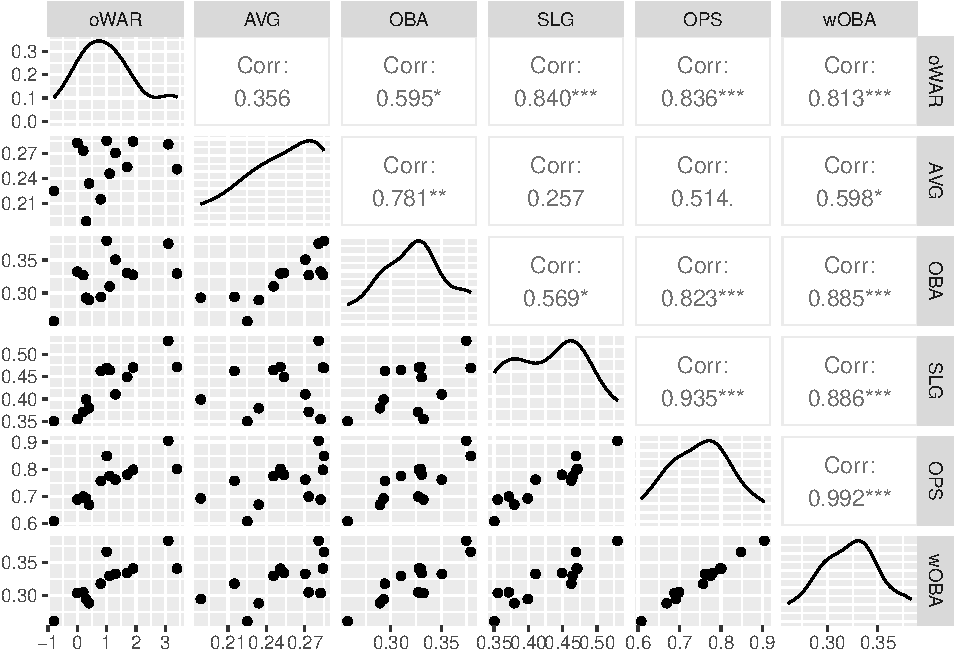
\includegraphics{textbook_files/figure-latex/unnamed-chunk-19-2.pdf}

\newpage

\hypertarget{evaluating-pitching-statistics}{%
\subsection{Evaluating Pitching Statistics}\label{evaluating-pitching-statistics}}

Earned run average (ERA) has been traditionally used to evaluate a pitcher, however, it has some flaws. First of all, it is highly dependent on the fielders playing behind the pitcher. If a pitcher's shortstop has poor range, he won't convert as many groundballs into outs as a shortstop with good range. ERA is also a noisy measurement in that can be affected easily by random luck.

To overcome some of the downsides of ERA, FIP and xFIP were developed to help reduce the variance (noise) of the measurement and to remove factors, like defense, that are not a function of the pitcher's ability.

Let's look at the twenty starting pitchers that had the most innings pitched in MLB for the total of the 2020 and 2021 seasons. We want to examine the year-to-year correlation between ERA, FIP, and xFIP.

\begin{Shaded}
\begin{Highlighting}[]
\NormalTok{pitchers2021 }\OtherTok{\textless{}{-}} \FunctionTok{read\_csv}\NormalTok{(}\StringTok{"data/MLBpitchers20{-}21.csv"}\NormalTok{)}
\NormalTok{pitchers2021 }\SpecialCharTok{\%\textgreater{}\%} \FunctionTok{slice\_head}\NormalTok{(}\AttributeTok{n=}\DecValTok{5}\NormalTok{) }\SpecialCharTok{\%\textgreater{}\%} \FunctionTok{kt}\NormalTok{()}
\end{Highlighting}
\end{Shaded}

\begin{table}[H]
\centering
\begin{tabular}{lrrrrrr}
\toprule
Player & ERA20 & FIP20 & xFIP20 & ERA21 & FIP21 & xFIP21\\
\midrule
Zack Wheeler & 2.92 & 3.22 & 3.76 & 2.78 & 2.59 & 2.84\\
Adam Wainwright & 3.15 & 4.11 & 4.23 & 3.05 & 3.66 & 3.87\\
Kyle Hendricks & 2.88 & 3.55 & 3.78 & 0.77 & 4.89 & 4.61\\
German Marquez & 3.75 & 3.28 & 3.83 & 4.40 & 3.86 & 3.64\\
Luis Castillo & 3.21 & 2.65 & 2.82 & 3.98 & 3.75 & 3.63\\
\bottomrule
\end{tabular}
\end{table}

\vfill
\newpage

Let's look at the correlations between these variables, paying close attention to what variables are most correlated with ERA20, a pitcher's ERA in 2020.

\begin{Shaded}
\begin{Highlighting}[]
\NormalTok{pitchers2021 }\SpecialCharTok{\%\textgreater{}\%}
  \FunctionTok{select}\NormalTok{(}\SpecialCharTok{{-}}\NormalTok{Player) }\SpecialCharTok{\%\textgreater{}\%}
  \FunctionTok{ggpairs}\NormalTok{(}\AttributeTok{title=}\StringTok{"Correlation plot of pitching statistics, MLB 2020{-}2021"}\NormalTok{)}
\end{Highlighting}
\end{Shaded}

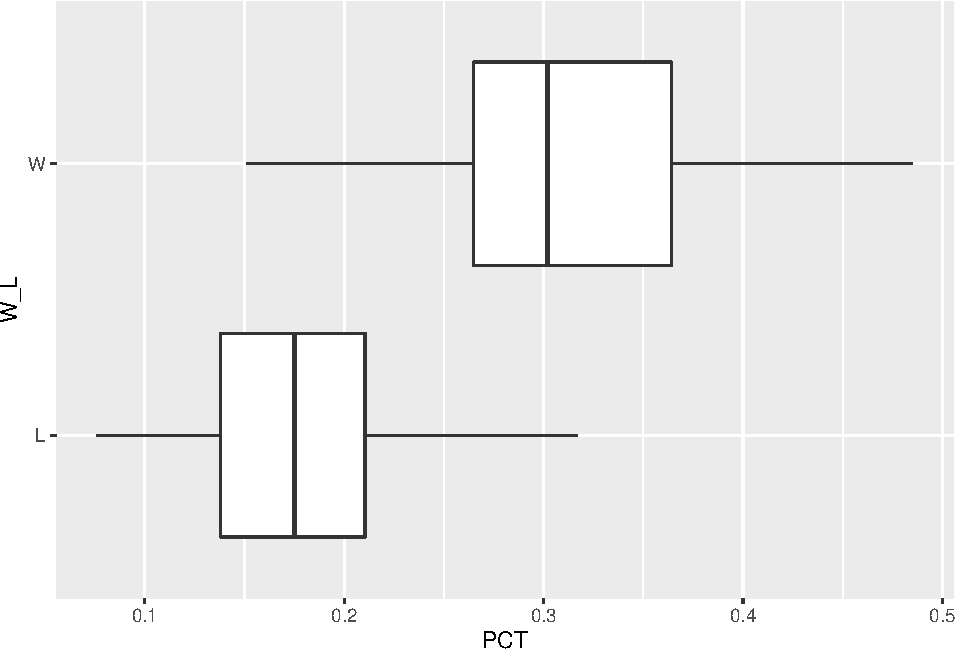
\includegraphics{textbook_files/figure-latex/unnamed-chunk-21-1.pdf}

This is a small dataset that only contains twenty pitchers (samples), but you will notice that ERA20 is more highly correlated with FIP21 and xFIP21 than ERA21. In other words, FIP and xFIP are likely better predictors of ERA success in the future rather than ERA success in the past.

\vfill
\newpage

\hypertarget{football}{%
\section{Football}\label{football}}

\href{https://www.youtube.com/watch?v=Ddwp1HyEFRE}{Link to YouTube video describing football rules}

\hypertarget{basic-football-statistics}{%
\subsection{Basic Football Statistics}\label{basic-football-statistics}}

\begin{itemize}
\item
  \textbf{Yards} (Yd): Number of yards gained from the line of scrimmage (can be broken down into Offense: Rushing and Passing Yards, Defense: Rushing and Passing Yards Allowed, and Special Teams: Kick and Punt Return Yards)
\item
  \textbf{Touchdowns} (TD): Number of times the offense carries or passes the ball successfully into the end zone of the opposing side (can be broken down into: Offensive TDs: Rushing and Passing TDs, Defensive TDs: interception or fumble recovery for a touchdown, and Special Teams TDs: kick or punt return touchdowns)
\item
  \textbf{Sacks} (Sk): Number of times a player or a team tackles the quarterback behind the line of scrimmage before he can throw a pass
\item
  \textbf{Interceptions} (INT): Number of times a player or a team catches an opponent's pass
\end{itemize}

\hypertarget{advanced-football-statistics}{%
\subsection{Advanced Football Statistics}\label{advanced-football-statistics}}

\begin{itemize}
\tightlist
\item
  \textbf{Passer Rating (or Passing Efficiency)}: Measure of performance of a quarterback
\end{itemize}

For NFL, the formula is as follows:\\

\[Passer Rating_{NFL} = \left(\frac{a+b+c+d}{6}\right) \cdot 100\]

where:
\[a = \left(\frac{COMP}{ATT}-0.3\right) \cdot 5\]
\[b = \left(\frac{YDS}{ATT} - 3\right) \cdot 0.25\]
\[c = \left(\frac{TD}{ATT}\right) \cdot 20\]
\[d = 2.375 - \left(\frac{INT}{ATT} \cdot 25\right)\]

ATT = Number of passing attempts, COMP = Number of completions, YDS = Passing yards, TD = Touchdown passes, INT = Interceptions\\

\emph{Note:} If the result of any calculation is greater than 2.375, it is set to 2.375. If the result is a negative number, it is set to zero.\\

For College Football, the formula is as follows:\\

\[Passer Rating_{NCAAF} = \frac{(8.4 \cdot YDS) + (330 \cdot TD) + (100 \cdot COMP) - (200 \cdot INT)}{ATT}\]

\begin{itemize}
\item
  \textbf{Total Quarterback Rating} (QBR): Proprietary measure of performance of a quarterback developed by ESPN in 2011. This is a more comprehensive measurement of quarterback performance that accounts for the quarterback's impact on his team's passes, rushes, turnovers, and penalties in terms of \textbf{expected points added}.
\item
  \textbf{Expected Points Added} (EPA): Measure of how many points a player or a play is worth to a team.
\end{itemize}

\emph{References:}\\
\url{https://www.pro-football-reference.com/about/glossary.htm}\strut \\
\url{https://en.wikipedia.org/wiki/Passer_rating}

\newpage

\begin{example}
Individual NFL quarterback passing statistics for the 2021 season are provided in \texttt{NFL\_Ind\_Passing\_2021.csv}. Note that this dataset only includes quarterbacks with at least 100 passing yards in 2021. Passer efficiency is given in the \texttt{RTG} column.
\end{example}

\begin{Shaded}
\begin{Highlighting}[]
\CommentTok{\# Data: https://www.espn.com/nfl/stats/player}
\NormalTok{QB\_21 }\OtherTok{\textless{}{-}} \FunctionTok{read\_csv}\NormalTok{(}\StringTok{"data/NFL\_Ind\_Passing\_2021.csv"}\NormalTok{)}
\NormalTok{QB\_21 }\SpecialCharTok{\%\textgreater{}\%} \FunctionTok{select}\NormalTok{(}\DecValTok{1}\NormalTok{,}\DecValTok{3}\SpecialCharTok{:}\DecValTok{8}\NormalTok{,}\DecValTok{11}\SpecialCharTok{:}\DecValTok{12}\NormalTok{,}\DecValTok{15}\SpecialCharTok{:}\DecValTok{16}\NormalTok{) }\SpecialCharTok{\%\textgreater{}\%} \FunctionTok{slice\_head}\NormalTok{(}\AttributeTok{n=}\DecValTok{10}\NormalTok{) }\SpecialCharTok{\%\textgreater{}\%} \FunctionTok{kt}\NormalTok{()}
\end{Highlighting}
\end{Shaded}

\begin{table}[H]
\centering
\begin{tabular}{lrrrrrrrrrr}
\toprule
Name & GP & CMP & ATT & CMP\% & YDS & AVG & TD & INT & QBR & RTG\\
\midrule
Tom Brady & 17 & 485 & 719 & 67.5 & 5316 & 7.4 & 43 & 12 & 68.1 & 102.1\\
Justin Herbert & 17 & 443 & 672 & 65.9 & 5014 & 7.5 & 38 & 15 & 65.6 & 97.7\\
Patrick Mahomes & 17 & 436 & 658 & 66.3 & 4839 & 7.4 & 37 & 13 & 62.2 & 98.5\\
Josh Allen & 17 & 409 & 646 & 63.3 & 4407 & 6.8 & 36 & 15 & 60.7 & 92.2\\
Derek Carr & 17 & 428 & 626 & 68.4 & 4804 & 7.7 & 23 & 14 & 52.4 & 94.0\\
Ben Roethlisberger & 16 & 390 & 605 & 64.5 & 3740 & 6.2 & 22 & 10 & 35.6 & 86.8\\
Trevor Lawrence & 17 & 359 & 602 & 59.6 & 3641 & 6.0 & 12 & 17 & 33.5 & 71.9\\
Matthew Stafford & 17 & 404 & 601 & 67.2 & 4886 & 8.1 & 41 & 17 & 63.8 & 102.9\\
Dak Prescott & 16 & 410 & 596 & 68.8 & 4449 & 7.5 & 37 & 10 & 54.6 & 104.2\\
Kirk Cousins & 16 & 372 & 561 & 66.3 & 4221 & 7.5 & 33 & 7 & 52.3 & 103.1\\
\bottomrule
\end{tabular}
\end{table}

\begin{Shaded}
\begin{Highlighting}[]
\FunctionTok{names}\NormalTok{(QB\_21)}
\end{Highlighting}
\end{Shaded}

\begin{verbatim}
##  [1] "Name"  "Team"  "GP"    "CMP"   "ATT"   "CMP%"  "YDS"   "AVG"   "YDS/G"
## [10] "LNG"   "TD"    "INT"   "SACK"  "SYL"   "QBR"   "RTG"
\end{verbatim}

\begin{enumerate}
\def\labelenumi{(\alph{enumi})}
\tightlist
\item
  Confirm this is passer rating by creating a new variable to calculate passer rating using the provided statistics.
\end{enumerate}

\begin{Shaded}
\begin{Highlighting}[]
\CommentTok{\# Create intermediate variables}
\NormalTok{QB\_21 }\OtherTok{\textless{}{-}}\NormalTok{ QB\_21 }\SpecialCharTok{\%\textgreater{}\%} 
  \FunctionTok{mutate}\NormalTok{(}\AttributeTok{a =}\NormalTok{ (CMP}\SpecialCharTok{/}\NormalTok{ATT}\FloatTok{{-}0.3}\NormalTok{)}\SpecialCharTok{*}\DecValTok{5}\NormalTok{) }\SpecialCharTok{\%\textgreater{}\%}
  \FunctionTok{mutate}\NormalTok{(}\AttributeTok{b =}\NormalTok{ (YDS}\SpecialCharTok{/}\NormalTok{ATT}\DecValTok{{-}3}\NormalTok{)}\SpecialCharTok{*}\FloatTok{0.25}\NormalTok{) }\SpecialCharTok{\%\textgreater{}\%}
  \FunctionTok{mutate}\NormalTok{(}\AttributeTok{c =}\NormalTok{ (TD}\SpecialCharTok{/}\NormalTok{ATT)}\SpecialCharTok{*}\DecValTok{20}\NormalTok{) }\SpecialCharTok{\%\textgreater{}\%}
  \FunctionTok{mutate}\NormalTok{(}\AttributeTok{d =} \FloatTok{2.375} \SpecialCharTok{{-}}\NormalTok{(INT}\SpecialCharTok{/}\NormalTok{ATT}\SpecialCharTok{*}\DecValTok{25}\NormalTok{))}

\CommentTok{\# Check to see if a,b,c,d are less than 0 or greater than 2.375}
\NormalTok{QB\_21 }\SpecialCharTok{\%\textgreater{}\%} \FunctionTok{summarize}\NormalTok{(}\FunctionTok{min}\NormalTok{(a),}\FunctionTok{max}\NormalTok{(a),}\FunctionTok{min}\NormalTok{(b),}\FunctionTok{max}\NormalTok{(b),}\FunctionTok{min}\NormalTok{(c),}\FunctionTok{max}\NormalTok{(c),}\FunctionTok{min}\NormalTok{(d),}\FunctionTok{max}\NormalTok{(d))}
\end{Highlighting}
\end{Shaded}

\begin{verbatim}
## # A tibble: 1 x 8
##   `min(a)` `max(a)` `min(b)` `max(b)` `min(c)` `max(c)` `min(d)` `max(d)`
##      <dbl>    <dbl>    <dbl>    <dbl>    <dbl>    <dbl>    <dbl>    <dbl>
## 1     1.19     2.02    0.433     1.47    0.319     1.74    0.860     2.19
\end{verbatim}

\begin{Shaded}
\begin{Highlighting}[]
\NormalTok{QB\_21 }\OtherTok{\textless{}{-}}\NormalTok{ QB\_21 }\SpecialCharTok{\%\textgreater{}\%}
  \FunctionTok{mutate}\NormalTok{(}\AttributeTok{PR =}\NormalTok{ (a}\SpecialCharTok{+}\NormalTok{b}\SpecialCharTok{+}\NormalTok{c}\SpecialCharTok{+}\NormalTok{d)}\SpecialCharTok{/}\DecValTok{6}\SpecialCharTok{*}\DecValTok{100}\NormalTok{)}

\NormalTok{QB\_21 }\SpecialCharTok{\%\textgreater{}\%} \FunctionTok{select}\NormalTok{(Name,RTG,PR) }\SpecialCharTok{\%\textgreater{}\%} \FunctionTok{slice\_head}\NormalTok{(}\AttributeTok{n=}\DecValTok{5}\NormalTok{) }\SpecialCharTok{\%\textgreater{}\%} \FunctionTok{kt}\NormalTok{()}
\end{Highlighting}
\end{Shaded}

\begin{table}[H]
\centering
\begin{tabular}{lrr}
\toprule
Name & RTG & PR\\
\midrule
Tom Brady & 102.1 & 102.083\\
Justin Herbert & 97.7 & 97.656\\
Patrick Mahomes & 98.5 & 98.455\\
Josh Allen & 92.2 & 92.170\\
Derek Carr & 94.0 & 93.963\\
\bottomrule
\end{tabular}
\end{table}

\begin{enumerate}
\def\labelenumi{(\alph{enumi})}
\setcounter{enumi}{1}
\tightlist
\item
  What counting statistics are most correlated with passer rating and with QBR?
\end{enumerate}

\begin{Shaded}
\begin{Highlighting}[]
\CommentTok{\# Grab the counting statistics and create a correlation plot with PR and QBR}
\NormalTok{QB\_21 }\SpecialCharTok{\%\textgreater{}\%} \FunctionTok{select}\NormalTok{(PR,QBR,CMP,ATT,YDS,TD,INT,SACK,SYL) }\SpecialCharTok{\%\textgreater{}\%} \FunctionTok{ggpairs}\NormalTok{()}
\end{Highlighting}
\end{Shaded}

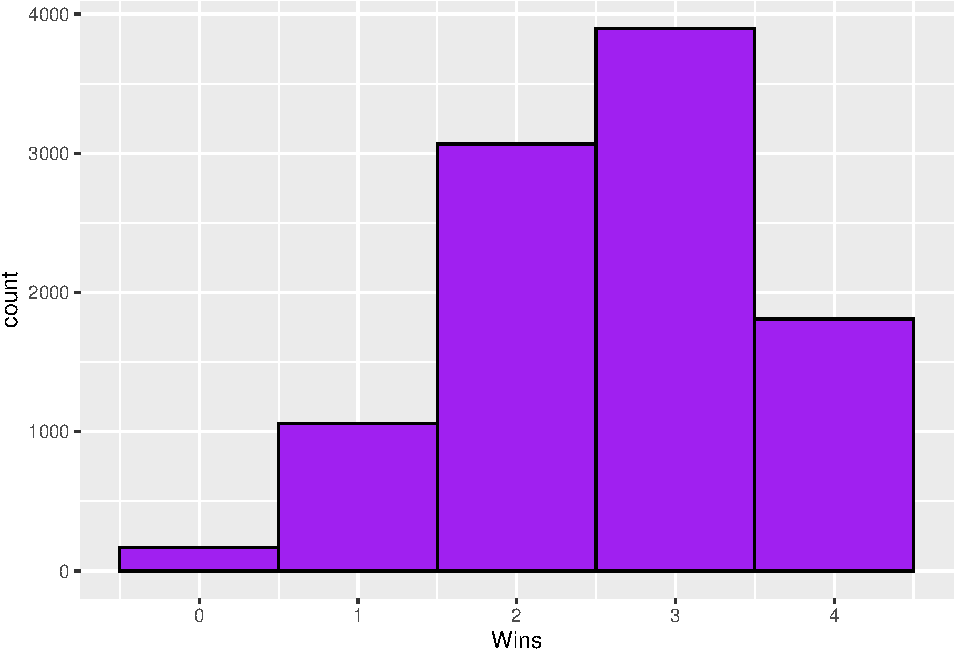
\includegraphics{textbook_files/figure-latex/unnamed-chunk-24-1.pdf}

\begin{enumerate}
\def\labelenumi{(\alph{enumi})}
\setcounter{enumi}{2}
\tightlist
\item
  What rate statistics are most correlated with passer efficiency and with QBR? Use CMP\% (completion percentage, completions per attempt), AVG (average yards per attempt), YDS/G (yards per game), and create new variables for interceptions per attempt, touchdowns per attempt, and sacks per attempt.
\end{enumerate}

\begin{Shaded}
\begin{Highlighting}[]
\CommentTok{\# Grab the counting statistics and create a correlation plot with PR and QBR}
\NormalTok{QB\_21 }\OtherTok{\textless{}{-}}\NormalTok{ QB\_21 }\SpecialCharTok{\%\textgreater{}\%} 
  \FunctionTok{mutate}\NormalTok{(}\AttributeTok{INTp =}\NormalTok{ INT}\SpecialCharTok{/}\NormalTok{ATT) }\SpecialCharTok{\%\textgreater{}\%}
  \FunctionTok{mutate}\NormalTok{(}\AttributeTok{TDp =}\NormalTok{ TD}\SpecialCharTok{/}\NormalTok{ATT) }\SpecialCharTok{\%\textgreater{}\%}
  \FunctionTok{mutate}\NormalTok{(}\AttributeTok{SACKp =}\NormalTok{ SACK}\SpecialCharTok{/}\NormalTok{ATT)}

\NormalTok{QB\_21 }\SpecialCharTok{\%\textgreater{}\%} \FunctionTok{select}\NormalTok{(PR,QBR,}\StringTok{\textasciigrave{}}\AttributeTok{CMP\%}\StringTok{\textasciigrave{}}\NormalTok{,AVG,}\StringTok{\textasciigrave{}}\AttributeTok{YDS/G}\StringTok{\textasciigrave{}}\NormalTok{,INTp,TDp,SACKp) }\SpecialCharTok{\%\textgreater{}\%} \FunctionTok{ggpairs}\NormalTok{()}
\end{Highlighting}
\end{Shaded}

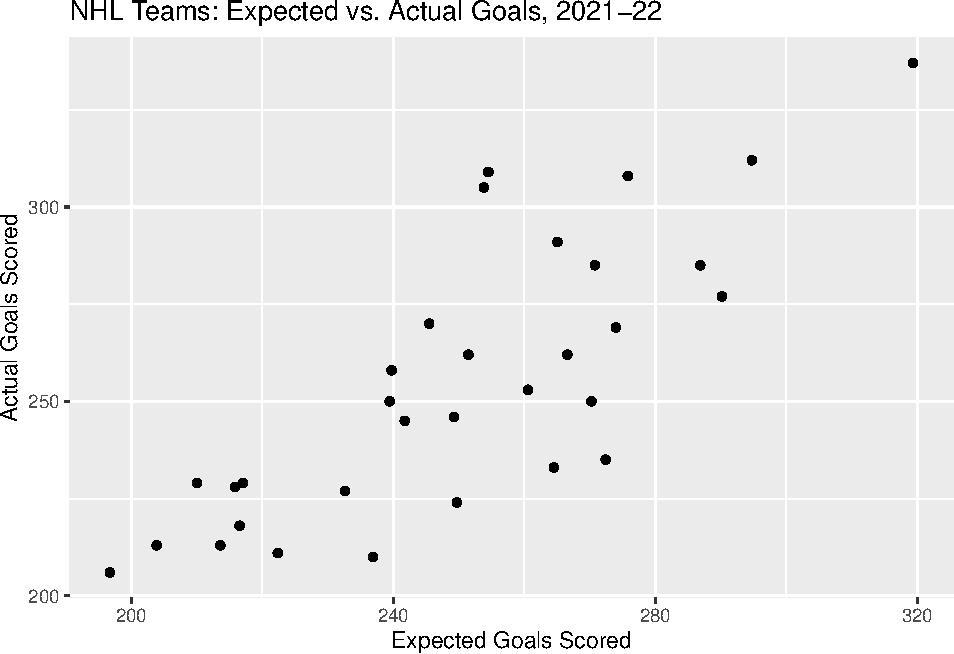
\includegraphics{textbook_files/figure-latex/unnamed-chunk-25-1.pdf}

\newpage

\hypertarget{basketball}{%
\section{Basketball}\label{basketball}}

\href{https://www.youtube.com/watch?v=wYjp2zoqQrs}{Link to YouTube video describing basketball rules}

\hypertarget{basic-basketball-statistics}{%
\subsection{Basic Basketball Statistics}\label{basic-basketball-statistics}}

\begin{itemize}
\item
  \textbf{Field Goal (FG)}: A made shot from either 2- or 3-point range. Free throws, worth 1 point, are not considered field goals. Field goal statistics often include attempts, makes, and percentage.
\item
  \textbf{Free Throw (FT)}: After certain fouls, the clock stops and a player shoots an uncontested shot from the foul line. These free throws are worth 1 point each; like with field goals, FT statistics often include attempts, makes, and percentage.
\item
  \textbf{Assists (AST)}: A player is credited with an assist if they pass the ball to a teammate and the teammate scores a field goal after zero or one dribbles. No more than one assist can be recorded per field goal.
\item
  \textbf{Turnover (TO)}: A player or team can be charged with a turnover for an action or violation that ends their offensive possession before being able to attempt a field goal. For a player (especially a guard), TOs can be compared to assists using Assist:Turnover ratio.
\item
  \textbf{Rebound (REB)}: The first player to gain control of the ball following a missed field goal is credited with a rebound. If the player is on the same team as the field goal shooter, it is an offensive rebound; otherwise, a defensive rebound.
\item
  \textbf{Points per Possession (PPP)}: Divides a team's points by number of possessions to account for a team's pace.
\end{itemize}

\hypertarget{advanced-basketball-statistics}{%
\subsection{Advanced Basketball Statistics}\label{advanced-basketball-statistics}}

\begin{itemize}
\item
  \textbf{True Shooting Percentage (TS\%)}: Unlike traditional shooting percentage, this statistic considers both field goals and free throws. It also gives more weight to shots that are worth more points.
\item
  \textbf{Win Shares}: Win shares give each player points for actions that contribute to a team's success. Win shares take into account a variety of offensive and defensive statistics, but can be calculated using different methods on different platforms.
\item
  \textbf{Value Over Replacement Player (VORP)}: This is basketball's response to baseball's WAR. VORP is a rate statistic that estimates a player's offensive output as compared to an ``average'' player.
\item
  \textbf{Player Efficiency Rating (PER)}: According to its creator John Hollinger,
  ``The PER sums up all a player's positive accomplishments, subtracts the negative accomplishments, and returns a per-minute rating of a player's performance.'' This statistic rewards great offensive performance more than great defensive plays.
\end{itemize}

\emph{References:}\\
\url{https://www.basketball-reference.com/about/per.html}\strut \\
\url{https://www.basketball-reference.com/about/ws.html}\strut \\
\url{https://www.basketball-reference.com/about/glossary.html}

\hypertarget{four-factors}{%
\subsection{Four Factors}\label{four-factors}}

Tibbles are a type of data frame supported by the \texttt{tidyverse} package. The following tibble contains data from a Mountain West tournament game played between the CSU and Wyoming women's basketball teams during the 2021-2022 season, which CSU won 51-38. \href{https://csurams.com/sports/womens-basketball/stats/2021-22/wyoming/boxscore/16095}{(Here's the link to the box score on the CSU athletics website.)}

\begin{Shaded}
\begin{Highlighting}[]
\NormalTok{basketball\_data }\OtherTok{\textless{}{-}} \FunctionTok{tibble}\NormalTok{(}\AttributeTok{team =} \FunctionTok{c}\NormalTok{(}\StringTok{"CSU"}\NormalTok{,}\StringTok{"WYO"}\NormalTok{), }\AttributeTok{FG =} \FunctionTok{c}\NormalTok{(}\DecValTok{14}\NormalTok{,}\DecValTok{15}\NormalTok{), }\AttributeTok{FGA =} \FunctionTok{c}\NormalTok{(}\DecValTok{48}\NormalTok{,}\DecValTok{60}\NormalTok{), }
                          \AttributeTok{THREEP =} \FunctionTok{c}\NormalTok{(}\DecValTok{5}\NormalTok{,}\DecValTok{4}\NormalTok{), }\AttributeTok{FT =} \FunctionTok{c}\NormalTok{(}\DecValTok{10}\NormalTok{,}\DecValTok{4}\NormalTok{), }\AttributeTok{FTA =} \FunctionTok{c}\NormalTok{(}\DecValTok{14}\NormalTok{,}\DecValTok{4}\NormalTok{), }
                          \AttributeTok{ORB =} \FunctionTok{c}\NormalTok{(}\DecValTok{2}\NormalTok{,}\DecValTok{14}\NormalTok{), }\AttributeTok{DRB =} \FunctionTok{c}\NormalTok{(}\DecValTok{31}\NormalTok{,}\DecValTok{30}\NormalTok{), }\AttributeTok{TOV =} \FunctionTok{c}\NormalTok{(}\DecValTok{5}\NormalTok{,}\DecValTok{12}\NormalTok{))}
\NormalTok{basketball\_data }\SpecialCharTok{\%\textgreater{}\%} \FunctionTok{kt}\NormalTok{()}
\end{Highlighting}
\end{Shaded}

\begin{table}[H]
\centering
\begin{tabular}{lrrrrrrrr}
\toprule
team & FG & FGA & THREEP & FT & FTA & ORB & DRB & TOV\\
\midrule
CSU & 14 & 48 & 5 & 10 & 14 & 2 & 31 & 5\\
WYO & 15 & 60 & 4 & 4 & 4 & 14 & 30 & 12\\
\bottomrule
\end{tabular}
\end{table}

This tibble contains all the data needed to calculate the \emph{Four Factors}. The Four Factors of a basketball game are statistics formulated by Dean Oliver, former Director of Quantitative Analysis for the Denver Nuggets (among other roles). These statistics are also promoted by sports data platforms like Hudl.com.

The Four Factors each have offensive and defensive versions; for this example, we'll focus on the offensive perspective.

\begin{enumerate}
\def\labelenumi{\arabic{enumi}.}
\tightlist
\item
  \textbf{\emph{Scoring}}: \textbf{Effective Field Goal Percentage} (eFG\%)
\end{enumerate}

\(eFG\% = \frac{FG\ +\ 0.5(3P)}{FGA}\)

\begin{enumerate}
\def\labelenumi{\arabic{enumi}.}
\setcounter{enumi}{1}
\tightlist
\item
  \textbf{\emph{Crashing}}: \textbf{Turnover Percentage} (TOV\%)
\end{enumerate}

\(TOV\% = \frac{TOV}{FGA\ +\ 0.44(FTA)\ +\ TOV}\)

\begin{enumerate}
\def\labelenumi{\arabic{enumi}.}
\setcounter{enumi}{2}
\tightlist
\item
  \textbf{\emph{Protecting}}: \textbf{Rebounding Percentage} (ORB\%)
\end{enumerate}

\(ORB\% = \frac{ORB}{ORB\ +\ Opponent\ DRB}\)

\begin{enumerate}
\def\labelenumi{\arabic{enumi}.}
\setcounter{enumi}{3}
\tightlist
\item
  \textbf{\emph{Attacking}}: \textbf{Free Throw Factor} (FT Factor)
\end{enumerate}

\(FT\ factor = \frac{FT}{FGA}\)

Let's calculate the values of eFG\%, TOV\%, ORB\%, and Free Throw Factor for both CSU and Wyoming and add them as new columns in the tibble using the \texttt{add\_column} function.

\begin{Shaded}
\begin{Highlighting}[]
\NormalTok{basketball\_data }\OtherTok{\textless{}{-}}\NormalTok{ basketball\_data }\SpecialCharTok{\%\textgreater{}\%} 
  \FunctionTok{mutate}\NormalTok{(}\AttributeTok{eFG =} \DecValTok{100}\SpecialCharTok{*}\NormalTok{(FG }\SpecialCharTok{+}\NormalTok{ .}\DecValTok{5} \SpecialCharTok{*}\NormalTok{ THREEP)}\SpecialCharTok{/}\NormalTok{FGA) }\SpecialCharTok{\%\textgreater{}\%}
  \FunctionTok{mutate}\NormalTok{(}\AttributeTok{TOVPCT =} \DecValTok{100}\SpecialCharTok{*}\NormalTok{(FG }\SpecialCharTok{+}\NormalTok{ .}\DecValTok{5} \SpecialCharTok{*}\NormalTok{ THREEP)}\SpecialCharTok{/}\NormalTok{FGA) }\SpecialCharTok{\%\textgreater{}\%}
  \FunctionTok{mutate}\NormalTok{(}\AttributeTok{ORBPCT =} \DecValTok{100}\SpecialCharTok{*}\FunctionTok{c}\NormalTok{(ORB[}\DecValTok{1}\NormalTok{]}\SpecialCharTok{/}\NormalTok{(ORB[}\DecValTok{1}\NormalTok{]}\SpecialCharTok{+}\NormalTok{DRB[}\DecValTok{2}\NormalTok{]), ORB[}\DecValTok{2}\NormalTok{]}\SpecialCharTok{/}\NormalTok{(ORB[}\DecValTok{2}\NormalTok{]}\SpecialCharTok{+}\NormalTok{DRB[}\DecValTok{1}\NormalTok{]))) }\SpecialCharTok{\%\textgreater{}\%}
  \FunctionTok{mutate}\NormalTok{(}\AttributeTok{FTFACTOR =} \DecValTok{100}\SpecialCharTok{*}\NormalTok{FT}\SpecialCharTok{/}\NormalTok{FGA)}

\NormalTok{basketball\_data }\SpecialCharTok{\%\textgreater{}\%} \FunctionTok{select}\NormalTok{(team,eFG, TOVPCT, ORBPCT, FTFACTOR) }\SpecialCharTok{\%\textgreater{}\%} \FunctionTok{kt}\NormalTok{()}
\end{Highlighting}
\end{Shaded}

\begin{table}[H]
\centering
\begin{tabular}{lrrrr}
\toprule
team & eFG & TOVPCT & ORBPCT & FTFACTOR\\
\midrule
CSU & 34.375 & 34.375 & 6.250 & 20.833\\
WYO & 28.333 & 28.333 & 31.111 & 6.667\\
\bottomrule
\end{tabular}
\end{table}

While this method does produce Four Factors data, it could be difficult to scale for calculating the same statistics for a sample of several games. In the next section, we will introduce an \texttt{R} package that aids in the calculation of Four Factors.

\hypertarget{basketballanalyzer-four-factors}{%
\subsubsection{BasketballAnalyzeR Four Factors}\label{basketballanalyzer-four-factors}}

The authors of ``Basketball Data Science With Applications in R'' developed the \texttt{BasketballAnalyzeR} package to be used in conjunction with the book. \texttt{BasketballAnalyzeR} includes built-in datasets from the 2017-18 NBA season and provides many functions for analyzing and plotting basketball data. One such function is \texttt{fourfactors}, which offers a simpler way to perform a four factors analysis.

\begin{Shaded}
\begin{Highlighting}[]
\FunctionTok{library}\NormalTok{(}\StringTok{"BasketballAnalyzeR"}\NormalTok{)}

\NormalTok{teams }\OtherTok{\textless{}{-}} \FunctionTok{c}\NormalTok{(}\StringTok{"DEN"}\NormalTok{, }\StringTok{"CLE"}\NormalTok{, }\StringTok{"GSW"}\NormalTok{) }\CommentTok{\#Nuggets, Cavaliers, Warriors}
\NormalTok{team\_data }\OtherTok{\textless{}{-}} \FunctionTok{which}\NormalTok{(Tadd}\SpecialCharTok{$}\NormalTok{team }\SpecialCharTok{\%in\%}\NormalTok{ teams)}
\NormalTok{four\_factors\_teams }\OtherTok{\textless{}{-}} \FunctionTok{fourfactors}\NormalTok{(Tbox[team\_data, ], Obox[team\_data, ])}
\NormalTok{four\_factors\_teams }\SpecialCharTok{\%\textgreater{}\%} \FunctionTok{select}\NormalTok{(}\DecValTok{1}\NormalTok{,}\DecValTok{8}\SpecialCharTok{:}\DecValTok{15}\NormalTok{) }\SpecialCharTok{\%\textgreater{}\%} \FunctionTok{kt}\NormalTok{()}
\end{Highlighting}
\end{Shaded}

\begin{table}[H]
\centering
\begin{tabular}{lrrrrrrrr}
\toprule
Team & F1.Off & F2.Off & F3.Off & F4.Off & F1.Def & F2.Def & F3.Def & F4.Def\\
\midrule
Cleveland Cavaliers & 54.70 & 13.70 & 20.06 & 21.41 & 53.98 & 13.43 & 77.27 & 16.58\\
Denver Nuggets & 53.62 & 14.90 & 25.66 & 19.77 & 53.88 & 13.83 & 77.45 & 17.35\\
Golden State Warriors & 56.91 & 15.26 & 21.05 & 19.48 & 50.44 & 13.89 & 76.31 & 18.55\\
\bottomrule
\end{tabular}
\end{table}

This is a much simpler and neater way to calculate Four Factors.

In the 2017-18 season, the Warriors and Cavaliers met in the NBA Finals, while the Nuggets just missed the playoffs. It would be expected that the two Finals teams would have higher values for the Four Factors. While this is mostly true, for which of the Four Factors did the Nuggets have the highest value?

A: Factor 3 (rebounding percentage), both offensive and defensive.

\hypertarget{shot-charts}{%
\subsection{Shot Charts}\label{shot-charts}}

The \texttt{BasketballAnalyzeR} package includes shot location data for all players for the 2017-18 NBA season and has a function called \texttt{shotchart} that allows for the plotting of shot data.

Let's plot shot location data for Nikola Jokic. First, the coordinates must be transformed so that the point (0,0) is located at the corner of the court; the original coordinates place the origin at the center of the hoop.

\begin{Shaded}
\begin{Highlighting}[]
\NormalTok{PbP }\OtherTok{\textless{}{-}} \FunctionTok{PbPmanipulation}\NormalTok{(PbP.BDB)}

\NormalTok{jokic\_data }\OtherTok{\textless{}{-}} \FunctionTok{subset}\NormalTok{(PbP, player }\SpecialCharTok{==} \StringTok{"Nikola Jokic"}\NormalTok{)}
\NormalTok{jokic\_data}\SpecialCharTok{$}\NormalTok{xx }\OtherTok{\textless{}{-}}\NormalTok{ jokic\_data}\SpecialCharTok{$}\NormalTok{original\_x}\SpecialCharTok{/}\DecValTok{10} \CommentTok{\#transformation}
\NormalTok{jokic\_data}\SpecialCharTok{$}\NormalTok{yy }\OtherTok{\textless{}{-}}\NormalTok{ jokic\_data}\SpecialCharTok{$}\NormalTok{original\_y}\SpecialCharTok{/}\DecValTok{10} \SpecialCharTok{{-}} \FloatTok{41.75} \CommentTok{\#transformation}
\end{Highlighting}
\end{Shaded}

\texttt{BasketballAnalyzeR} supports three types of density visualizations within \texttt{shotchart}, one being \texttt{density-polygons}. Since \texttt{shotchart} is a \texttt{ggplot} object, a chart title can be added using \texttt{ggtitle}.

\begin{Shaded}
\begin{Highlighting}[]
\FunctionTok{shotchart}\NormalTok{(}\AttributeTok{data =}\NormalTok{ jokic\_data, }\AttributeTok{x=}\StringTok{"xx"}\NormalTok{, }\AttributeTok{y=}\StringTok{"yy"}\NormalTok{, }\AttributeTok{type=}\StringTok{"density{-}polygons"}\NormalTok{) }\SpecialCharTok{+} 
  \FunctionTok{ggtitle}\NormalTok{(}\StringTok{"Nikola Jokic Shot Data, 2017{-}18"}\NormalTok{)}
\end{Highlighting}
\end{Shaded}

\begin{verbatim}
## Warning: The dot-dot notation (`..level..`) was
## deprecated in ggplot2 3.4.0.
## i Please use `after_stat(level)`
##   instead.
## i The deprecated feature was likely used
##   in the BasketballAnalyzeR package.
##   Please report the issue to the
##   authors.
\end{verbatim}

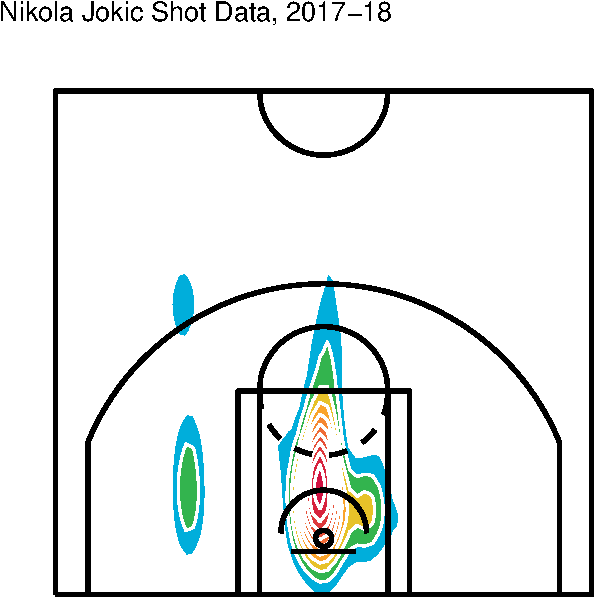
\includegraphics{textbook_files/figure-latex/basketballanalyzer 3-1.pdf}

It seems most shots attempts from Jokic were in the paint; this is hardly surprising, since he plays the center position. Here's the same chart with \texttt{density-hexbin}:

\begin{Shaded}
\begin{Highlighting}[]
\FunctionTok{shotchart}\NormalTok{(}\AttributeTok{data =}\NormalTok{ jokic\_data, }\AttributeTok{x=}\StringTok{"xx"}\NormalTok{, }\AttributeTok{y=}\StringTok{"yy"}\NormalTok{, }\AttributeTok{type=}\StringTok{"density{-}hexbin"}\NormalTok{) }\SpecialCharTok{+} 
  \FunctionTok{ggtitle}\NormalTok{(}\StringTok{"Nikola Jokic Shot Data, 2017{-}18"}\NormalTok{)}
\end{Highlighting}
\end{Shaded}

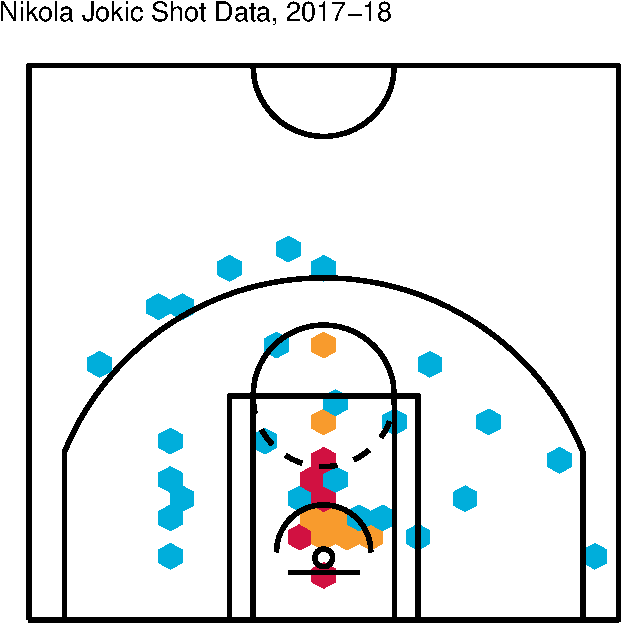
\includegraphics{textbook_files/figure-latex/basketballanalyzer 4-1.pdf}

The same chart with \texttt{density-raster}:

\begin{Shaded}
\begin{Highlighting}[]
\FunctionTok{shotchart}\NormalTok{(}\AttributeTok{data =}\NormalTok{ jokic\_data, }\AttributeTok{x=}\StringTok{"xx"}\NormalTok{, }\AttributeTok{y=}\StringTok{"yy"}\NormalTok{, }\AttributeTok{type=}\StringTok{"density{-}raster"}\NormalTok{) }\SpecialCharTok{+} 
  \FunctionTok{ggtitle}\NormalTok{(}\StringTok{"Nikola Jokic Shot Data, 2017{-}18"}\NormalTok{)}
\end{Highlighting}
\end{Shaded}

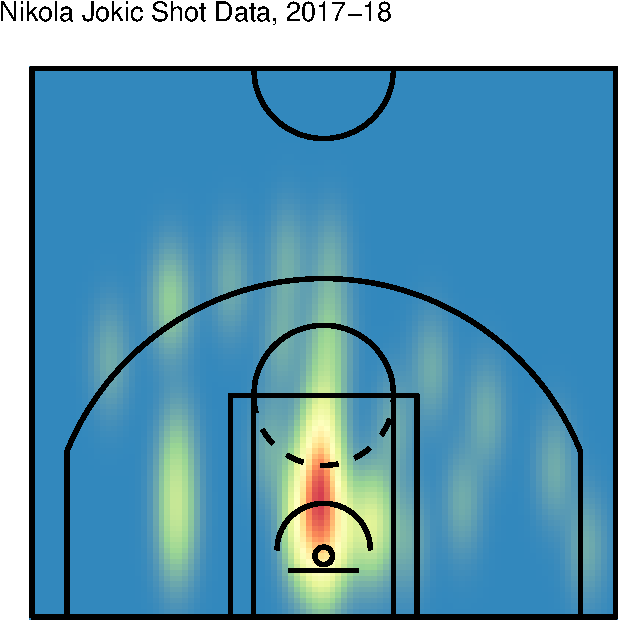
\includegraphics{textbook_files/figure-latex/basketballanalyzer 5-1.pdf}

Within the \texttt{shotchart} function, setting \texttt{scatter=TRUE} overlays the shots on the chart. Point size and transparency can also be customized.

\begin{Shaded}
\begin{Highlighting}[]
\FunctionTok{shotchart}\NormalTok{(}\AttributeTok{data =}\NormalTok{ jokic\_data, }\AttributeTok{x=}\StringTok{"xx"}\NormalTok{, }\AttributeTok{y=}\StringTok{"yy"}\NormalTok{, }\AttributeTok{type=}\StringTok{"density{-}raster"}\NormalTok{, }\AttributeTok{scatter=}\ConstantTok{TRUE}\NormalTok{) }\SpecialCharTok{+} 
  \FunctionTok{ggtitle}\NormalTok{(}\StringTok{"Nikola Jokic Shot Data, 2017{-}18"}\NormalTok{)}
\end{Highlighting}
\end{Shaded}

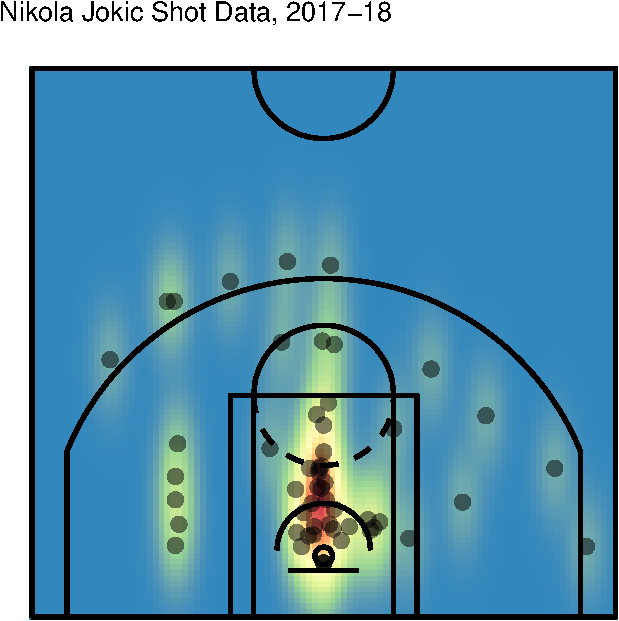
\includegraphics{textbook_files/figure-latex/basketballanalyzer 6-1.pdf}

Let's now compare shot charts of Nikola Jokic, Steph Curry, and Lebron James. This group of players includes one member of each team for which we calculated Four Factors.

\begin{Shaded}
\begin{Highlighting}[]
\NormalTok{curry\_data }\OtherTok{\textless{}{-}} \FunctionTok{subset}\NormalTok{(PbP, player }\SpecialCharTok{==} \StringTok{"Stephen Curry"}\NormalTok{)}
\NormalTok{curry\_data}\SpecialCharTok{$}\NormalTok{xx }\OtherTok{\textless{}{-}}\NormalTok{ curry\_data}\SpecialCharTok{$}\NormalTok{original\_x}\SpecialCharTok{/}\DecValTok{10} \CommentTok{\#transformation}
\NormalTok{curry\_data}\SpecialCharTok{$}\NormalTok{yy }\OtherTok{\textless{}{-}}\NormalTok{ curry\_data}\SpecialCharTok{$}\NormalTok{original\_y}\SpecialCharTok{/}\DecValTok{10} \SpecialCharTok{{-}} \FloatTok{41.75} \CommentTok{\#transformation}

\NormalTok{james\_data }\OtherTok{\textless{}{-}} \FunctionTok{subset}\NormalTok{(PbP, player }\SpecialCharTok{==} \StringTok{"LeBron James"}\NormalTok{)}
\NormalTok{james\_data}\SpecialCharTok{$}\NormalTok{xx }\OtherTok{\textless{}{-}}\NormalTok{ james\_data}\SpecialCharTok{$}\NormalTok{original\_x}\SpecialCharTok{/}\DecValTok{10} \CommentTok{\#transformation}
\NormalTok{james\_data}\SpecialCharTok{$}\NormalTok{yy }\OtherTok{\textless{}{-}}\NormalTok{ james\_data}\SpecialCharTok{$}\NormalTok{original\_y}\SpecialCharTok{/}\DecValTok{10} \SpecialCharTok{{-}} \FloatTok{41.75} \CommentTok{\#transformation}

\FunctionTok{shotchart}\NormalTok{(}\AttributeTok{data =}\NormalTok{ jokic\_data, }\AttributeTok{x=}\StringTok{"xx"}\NormalTok{, }\AttributeTok{y=}\StringTok{"yy"}\NormalTok{, }\AttributeTok{type=}\StringTok{"density{-}raster"}\NormalTok{) }\SpecialCharTok{+} 
  \FunctionTok{ggtitle}\NormalTok{(}\StringTok{"Nikola Jokic Shot Data, 2017{-}18"}\NormalTok{)}
\end{Highlighting}
\end{Shaded}

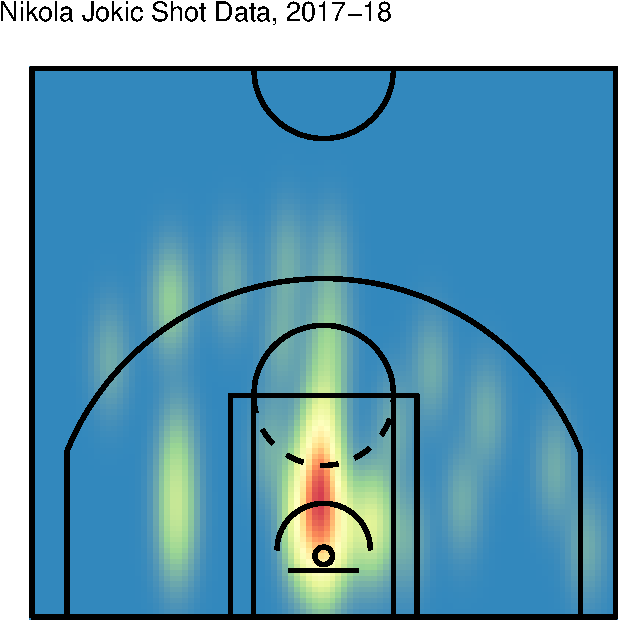
\includegraphics{textbook_files/figure-latex/basketballanalyzer 7-1.pdf}

\begin{Shaded}
\begin{Highlighting}[]
\FunctionTok{shotchart}\NormalTok{(}\AttributeTok{data =}\NormalTok{ curry\_data, }\AttributeTok{x=}\StringTok{"xx"}\NormalTok{, }\AttributeTok{y=}\StringTok{"yy"}\NormalTok{, }\AttributeTok{type=}\StringTok{"density{-}raster"}\NormalTok{) }\SpecialCharTok{+} 
  \FunctionTok{ggtitle}\NormalTok{(}\StringTok{"Steph Curry Shot Data, 2017{-}18"}\NormalTok{)}
\end{Highlighting}
\end{Shaded}

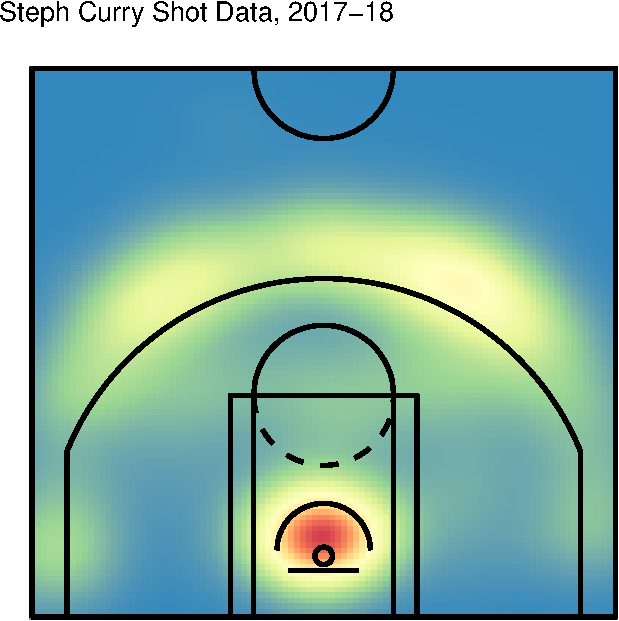
\includegraphics{textbook_files/figure-latex/basketballanalyzer 7-2.pdf}

\begin{Shaded}
\begin{Highlighting}[]
\FunctionTok{shotchart}\NormalTok{(}\AttributeTok{data =}\NormalTok{ james\_data, }\AttributeTok{x=}\StringTok{"xx"}\NormalTok{, }\AttributeTok{y=}\StringTok{"yy"}\NormalTok{, }\AttributeTok{type=}\StringTok{"density{-}raster"}\NormalTok{) }\SpecialCharTok{+} 
  \FunctionTok{ggtitle}\NormalTok{(}\StringTok{"Lebron James Shot Data, 2017{-}18"}\NormalTok{)}
\end{Highlighting}
\end{Shaded}

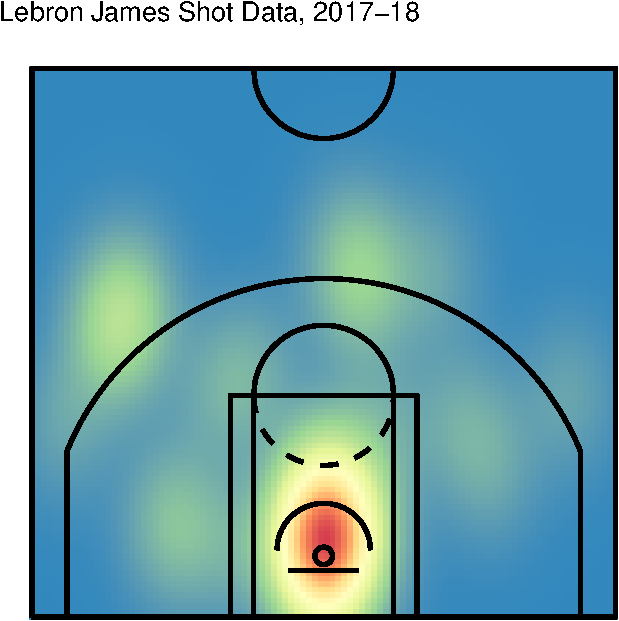
\includegraphics{textbook_files/figure-latex/basketballanalyzer 7-3.pdf}

Q: Of the three players (Jokic, Curry, James), which took the highest percentage of their three-point shots from the right side of the court (when facing the basket)?

A: Nikola Jokic shot almost all of his attempts from the right side. Steph Curry took many shots from beyond the arc and tended toward the left side, while James was split between the right side and the center.

Now, let's focus on Steph Curry's shooting. The following chart splits the court into zones based on angle and distance from the basket. The color in each zone represents the average length of the play leading up to that shot among shots taken in that zone.

\begin{Shaded}
\begin{Highlighting}[]
\FunctionTok{shotchart}\NormalTok{(}\AttributeTok{data =}\NormalTok{ curry\_data, }\AttributeTok{x=}\StringTok{"xx"}\NormalTok{, }\AttributeTok{y=}\StringTok{"yy"}\NormalTok{, }\AttributeTok{z=}\StringTok{"playlength"}\NormalTok{, }
          \AttributeTok{type=}\StringTok{"sectors"}\NormalTok{, }\AttributeTok{num.sect =} \DecValTok{7}\NormalTok{, }\AttributeTok{scatter=}\ConstantTok{TRUE}\NormalTok{, }\AttributeTok{pt.alpha=}\NormalTok{.}\DecValTok{3}\NormalTok{) }\SpecialCharTok{+} 
  \FunctionTok{ggtitle}\NormalTok{(}\StringTok{"Steph Curry Shot Data, 2017{-}18"}\NormalTok{)}
\end{Highlighting}
\end{Shaded}

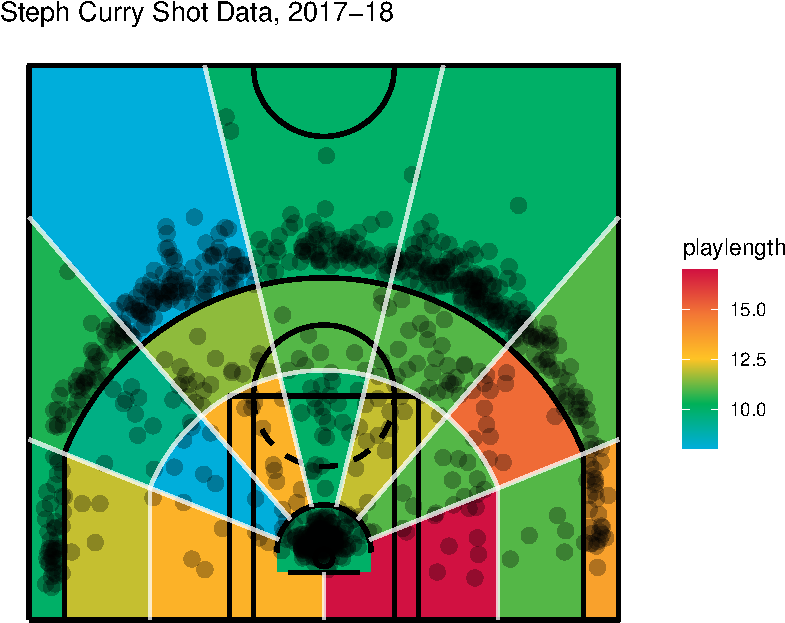
\includegraphics{textbook_files/figure-latex/basketballanalyzer 8-1.pdf}

Q: In general, did Steph Curry tend to shoot closer to the basket during plays of a longer duration or a shorter duration?

A: There is not a perfect correlation, but it seems that two-point field goals were attempted more often during longer plays, while shots taken outside the three-point arc were taken during plays of a shorter duration.

\emph{References:}
\url{https://rdrr.io/cran/BasketballAnalyzeR/}\\
Basketball Data Science (Zuccolotto and Manisera, 2020)

\newpage

\hypertarget{hockey}{%
\section{Hockey}\label{hockey}}

\href{https://www.youtube.com/watch?v=nv2FUnHceqU}{Link to YouTube video describing hockey rules}

\hypertarget{basic-hockey-statistics}{%
\subsection{Basic Hockey Statistics}\label{basic-hockey-statistics}}

Here are some basic statistics that are used often to describe hockey games.

\begin{itemize}
\item
  \textbf{Goals (G)}: If a team scores, the skater on the scoring team who last touched the puck is credited with a goal.
\item
  \textbf{Assists (A)}: The players (up to two) on the scoring team who last touch the puck before the goalscorer are credited with assists, unless the opposing team has possession of the puck in between.
\item
  \textbf{Points (PTS)}: Goals plus assists. {[}Not to be confused with team points awarded in the regular season standings by the many hockey leagues, including the NHL (two points for a win, one point for an overtime/shootout loss, zero points for a regulation loss){]}.
\item
  \textbf{Shots On Goal (SOG)}: Shot attempts in which the puck has been shot directly on goal. Shot attempts which are blocked or miss the goal are not considered SOGs. A team's shots on goal should equal the opposing goaltender's saves plus the team's goals scored.
\item
  \textbf{Goals Against Average (GAA)}: Of a goaltender, the number of goals allowed by that goaltender adjusted to a per-60 minute rate.
\item
  \textbf{Penalty Minutes (PIM)}: The amount of penalty time an individual player is assigned for their infractions. PIM may be different than the amount of time the player actually spends in the penalty box.
\end{itemize}

\emph{Reference:}\\
\url{https://www.milehighhockey.com/pages/stats}

\hypertarget{advanced-hockey-statistics}{%
\subsection{Advanced Hockey Statistics}\label{advanced-hockey-statistics}}

\begin{itemize}
\item
  \textbf{CORSI}: CORSI only applies to 5 on 5 (``even-strength'') situations. It is calculated as the difference between shot attempts on offense (shots on goal + blocked shots + missed shots) minus shot attempts allowed on defense. CORSI can also be expressed as a percentage, with percentages over 50\% indicating that the player is on ice for more offensive shots than defensive shots.
\item
  \textbf{Expected Goals (xG)}: Expected Goals statistics give each shot an estimated probability of scoring a goal based on factors such as shot location and game situation. xG cannot be less than 0 or greater than 1 for any particular shot, and different platforms may have different methods of calculating expected goals.
\item
  \textbf{Fenwick/Unblocked Shot Attempts (USAT)}: Similar to CORSI, but omits blocked shots from the calculation. This statistic is used in many Expected Goals calculations.
\end{itemize}

Because the flow of a hockey game is usually quite different in situations other than the normal 5 on 5, such as a power play (5 on 4) or concurrent penalties (4 on 4), many hockey databases separate data by the type of game situation. We will see this below with a dataset from \href{www.moneypuck.com}{MoneyPuck}, but it is also present on \href{https://www.naturalstattrick.com/}{Natural Stat Trick}, \href{www.quanthockey.com}{QuantHockey}, and \href{www.hockey-reference.com}{hockey-reference}.

\emph{References:}\\
\url{https://www.nhl.com/lightning/news/hockey-analytics-101-understanding-advanced-stats-and-how-theyre-measured/c-735819}\strut \\
\url{https://theathletic.com/121980/2017/10/09/an-advanced-stat-primer-understanding-basic-hockey-metrics/}

\hypertarget{actual-vs.-expected-goals}{%
\subsection{Actual vs.~Expected Goals}\label{actual-vs.-expected-goals}}

\begin{example}
For this example, we'll use a set of NHL data from moneypuck.com. First, let's load the data into \texttt{R} and open the data frame.
\end{example}

\begin{Shaded}
\begin{Highlighting}[]
\NormalTok{url }\OtherTok{\textless{}{-}} \StringTok{"https://moneypuck.com/moneypuck/playerData/seasonSummary/2021/regular/teams.csv"}
\NormalTok{nhl\_2022\_data }\OtherTok{\textless{}{-}} \FunctionTok{read\_csv}\NormalTok{(url)}

\NormalTok{nhl\_2022\_data }\SpecialCharTok{\%\textgreater{}\%} 
  \FunctionTok{slice\_head}\NormalTok{(}\AttributeTok{n=}\DecValTok{10}\NormalTok{) }\SpecialCharTok{\%\textgreater{}\%} 
  \FunctionTok{select}\NormalTok{(}\DecValTok{3}\NormalTok{,}\DecValTok{6}\NormalTok{,}\DecValTok{8}\NormalTok{,}\DecValTok{9}\NormalTok{,}\DecValTok{10}\NormalTok{) }\SpecialCharTok{\%\textgreater{}\%} \FunctionTok{kt}\NormalTok{()}
\end{Highlighting}
\end{Shaded}

\begin{table}[H]
\centering
\begin{tabular}{llrrr}
\toprule
name & situation & xGoalsPercentage & corsiPercentage & fenwickPercentage\\
\midrule
WPG & other & 0.49 & 0.50 & 0.47\\
WPG & all & 0.49 & 0.50 & 0.50\\
WPG & 5on5 & 0.49 & 0.49 & 0.50\\
WPG & 4on5 & 0.16 & 0.14 & 0.15\\
WPG & 5on4 & 0.86 & 0.86 & 0.85\\
CBJ & other & 0.52 & 0.49 & 0.49\\
CBJ & all & 0.45 & 0.48 & 0.47\\
CBJ & 5on5 & 0.45 & 0.48 & 0.47\\
CBJ & 4on5 & 0.14 & 0.18 & 0.21\\
CBJ & 5on4 & 0.81 & 0.84 & 0.82\\
\bottomrule
\end{tabular}
\end{table}

We can create nice looking tables using the ``kableExtra'\,' package. Let's look at the first eight rows and a small selection of columns of the data frame and format the table output using a kable table.

\begin{Shaded}
\begin{Highlighting}[]
\FunctionTok{library}\NormalTok{(}\StringTok{"kableExtra"}\NormalTok{)}

\NormalTok{nhl\_2022\_data[}\DecValTok{1}\SpecialCharTok{:}\DecValTok{8}\NormalTok{, }\FunctionTok{c}\NormalTok{(}\DecValTok{3}\NormalTok{,}\DecValTok{6}\SpecialCharTok{:}\DecValTok{9}\NormalTok{)] }\SpecialCharTok{\%\textgreater{}\%} \FunctionTok{kt}\NormalTok{()}
\end{Highlighting}
\end{Shaded}

\begin{table}[H]
\centering
\begin{tabular}{llrrr}
\toprule
name & situation & games\_played & xGoalsPercentage & corsiPercentage\\
\midrule
WPG & other & 82 & 0.49 & 0.50\\
WPG & all & 82 & 0.49 & 0.50\\
WPG & 5on5 & 82 & 0.49 & 0.49\\
WPG & 4on5 & 82 & 0.16 & 0.14\\
WPG & 5on4 & 82 & 0.86 & 0.86\\
CBJ & other & 82 & 0.52 & 0.49\\
CBJ & all & 82 & 0.45 & 0.48\\
CBJ & 5on5 & 82 & 0.45 & 0.48\\
\bottomrule
\end{tabular}
\end{table}

This dataset includes a \emph{lot} of covariates. It also splits these data by different game situations: even-strength (5 on 5), power play (5 on 4), etc. Let's subset the data to include all game situations.

Use the \texttt{nrow} command to check the number of columns in the new data frame. Check: Is it the same as the number of teams in the league for the 2021-2022 season?

\begin{Shaded}
\begin{Highlighting}[]
\NormalTok{nhl\_data\_all }\OtherTok{\textless{}{-}} \FunctionTok{filter}\NormalTok{(nhl\_2022\_data, situation }\SpecialCharTok{==} \StringTok{"all"}\NormalTok{)}

\FunctionTok{nrow}\NormalTok{(nhl\_data\_all)}
\end{Highlighting}
\end{Shaded}

\begin{verbatim}
## [1] 32
\end{verbatim}

The dataset includes an Expected Goals statistic for each team in the \texttt{xGoalsFor} column. Let's plot this quantity against the team's actual number of goals scored; this is given by the \texttt{goalsFor} column.

(Remember to always have a good title and axis labels!)

\begin{Shaded}
\begin{Highlighting}[]
\FunctionTok{ggplot}\NormalTok{(}\AttributeTok{data=}\NormalTok{nhl\_data\_all, }\FunctionTok{aes}\NormalTok{(}\AttributeTok{x=}\NormalTok{xGoalsFor, }\AttributeTok{y=}\NormalTok{goalsFor)) }\SpecialCharTok{+} 
  \FunctionTok{geom\_point}\NormalTok{() }\SpecialCharTok{+} 
  \FunctionTok{ggtitle}\NormalTok{(}\StringTok{"NHL Teams: Expected vs. Actual Goals, 2021{-}22"}\NormalTok{) }\SpecialCharTok{+}
  \FunctionTok{xlab}\NormalTok{(}\StringTok{"Expected Goals Scored"}\NormalTok{) }\SpecialCharTok{+}
  \FunctionTok{ylab}\NormalTok{(}\StringTok{"Actual Goals Scored"}\NormalTok{) }
\end{Highlighting}
\end{Shaded}

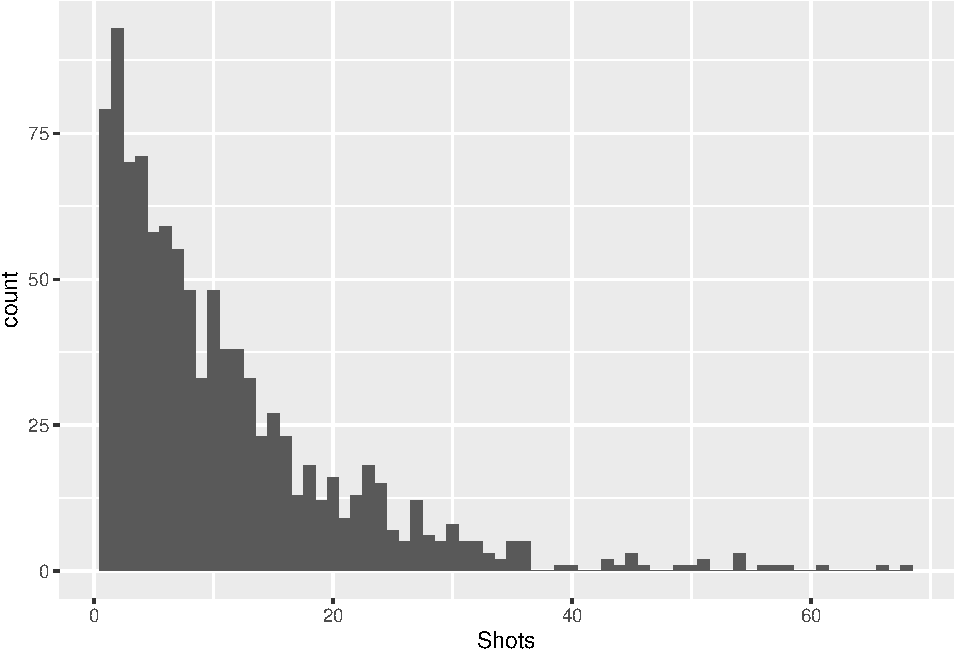
\includegraphics{textbook_files/figure-latex/unnamed-chunk-28-1.pdf}

As expected, there is a general positive correlation between expected and actual goals (\(r \approx 0.8\)). However, there is some variability - for example, the Kings only scored 7 more actual goals than the Ducks, despite having 56.6 more expected goals.

Let's add a line to the graph using the \texttt{geom\_abline} function corresponding to the line \(y=x\), the line on which data points would fall if expected goals were equal to actual goals. We can also customize the line's color and type.

\begin{Shaded}
\begin{Highlighting}[]
\FunctionTok{ggplot}\NormalTok{(}\AttributeTok{data=}\NormalTok{nhl\_data\_all, }\FunctionTok{aes}\NormalTok{(}\AttributeTok{x=}\NormalTok{xGoalsFor, }\AttributeTok{y=}\NormalTok{goalsFor)) }\SpecialCharTok{+} 
  \FunctionTok{geom\_point}\NormalTok{() }\SpecialCharTok{+} 
  \FunctionTok{geom\_abline}\NormalTok{(}\AttributeTok{intercept=}\DecValTok{0}\NormalTok{, }\AttributeTok{slope=}\DecValTok{1}\NormalTok{, }\AttributeTok{color=}\StringTok{"red"}\NormalTok{, }\AttributeTok{linetype=}\StringTok{"dashed"}\NormalTok{) }\SpecialCharTok{+} 
  \FunctionTok{ggtitle}\NormalTok{(}\StringTok{"NHL Teams: Expected vs. Actual Goals, 2021{-}22"}\NormalTok{) }\SpecialCharTok{+}
  \FunctionTok{xlab}\NormalTok{(}\StringTok{"Expected Goals Scored"}\NormalTok{) }\SpecialCharTok{+}
  \FunctionTok{ylab}\NormalTok{(}\StringTok{"Actual Goals Scored"}\NormalTok{) }
\end{Highlighting}
\end{Shaded}

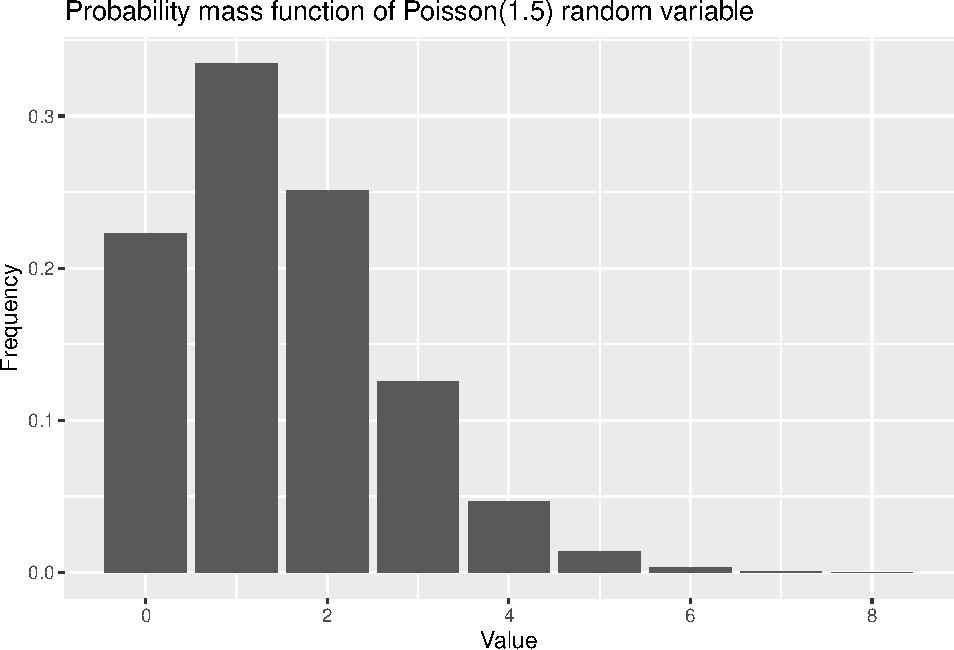
\includegraphics{textbook_files/figure-latex/unnamed-chunk-29-1.pdf}

\emph{Note: A slope of 0 and an intercept of 1 are actually the default parameters for the function.}

What does it mean for a team's data point to fall below this line? Above it?

\hfill\break
\hfill\break
\hfill\break
\hfill\break

Do you think that a team's expected goals would be more likely to be closer to its actual goals for a ten-game stretch, an entire season, or five consecutive seasons? Why?

\hfill\break
\hfill\break
\hfill\break
\hfill\break

\hypertarget{goalie-statistics}{%
\subsection{Goalie Statistics}\label{goalie-statistics}}

\begin{example}
For this next example, let's use goalie data from the 2021-2022 season from \href{https://www.naturalstattrick.com/}{Natural Stat Trick}.
\end{example}

\begin{Shaded}
\begin{Highlighting}[]
\NormalTok{goalie\_data }\OtherTok{\textless{}{-}} \FunctionTok{read.csv}\NormalTok{(}\StringTok{"data/GoalieTotals\_NaturalStatTrick.csv"}\NormalTok{)}
\NormalTok{goalie\_data }\SpecialCharTok{\%\textgreater{}\%} 
  \FunctionTok{select}\NormalTok{(}\DecValTok{2}\NormalTok{,}\DecValTok{3}\NormalTok{,}\DecValTok{4}\NormalTok{,}\DecValTok{5}\NormalTok{,}\DecValTok{6}\NormalTok{,}\DecValTok{7}\NormalTok{,}\DecValTok{8}\NormalTok{,}\DecValTok{12}\NormalTok{) }\SpecialCharTok{\%\textgreater{}\%} 
  \FunctionTok{arrange}\NormalTok{(}\SpecialCharTok{{-}}\NormalTok{TOI) }\SpecialCharTok{\%\textgreater{}\%} 
  \FunctionTok{slice\_head}\NormalTok{(}\AttributeTok{n=}\DecValTok{10}\NormalTok{) }\SpecialCharTok{\%\textgreater{}\%} 
  \FunctionTok{kt}\NormalTok{()}
\end{Highlighting}
\end{Shaded}

\begin{table}[H]
\centering
\begin{tabular}{llrrrrrr}
\toprule
Player & Team & GP & TOI & Shots.Against & Saves & Goals.Against & xG.Against\\
\midrule
Juuse Saros & NSH & 67 & 3931.383 & 2107 & 1934 & 173 & 180.69\\
Connor Hellebuyck & WPG & 66 & 3903.500 & 2155 & 1962 & 193 & 199.26\\
Andrei Vasilevskiy & T.B & 63 & 3760.750 & 1869 & 1713 & 156 & 165.89\\
Thatcher Demko & VAN & 64 & 3699.550 & 1967 & 1799 & 168 & 173.26\\
Jacob Markstrom & CGY & 63 & 3695.833 & 1754 & 1617 & 137 & 152.26\\
Tristan Jarry & PIT & 58 & 3414.717 & 1711 & 1573 & 138 & 143.92\\
Elvis Merzlikins & CBJ & 59 & 3320.400 & 1922 & 1744 & 178 & 164.94\\
Marc-Andre Fleury & CHI, MIN & 56 & 3284.867 & 1732 & 1573 & 159 & 148.00\\
Darcy Kuemper & COL & 57 & 3258.117 & 1755 & 1617 & 138 & 154.23\\
John Gibson & ANA & 56 & 3235.583 & 1789 & 1617 & 172 & 163.53\\
\bottomrule
\end{tabular}
\end{table}

The dataset includes 119 goalies, but many of them didn't play very much. We can subset the data to include only goaltenders that faced at least 500 shots.

Which player among qualified goalies had the best goals against average? On which team did he play, and what was his GAA?

Which goalie had the most playing time? What was his team, and how much time did he spend on the ice?

\begin{Shaded}
\begin{Highlighting}[]
\NormalTok{filtered\_goalie\_data }\OtherTok{\textless{}{-}} \FunctionTok{filter}\NormalTok{(goalie\_data, Shots.Against }\SpecialCharTok{\textgreater{}=} \DecValTok{500}\NormalTok{)}

\NormalTok{filtered\_goalie\_data }\SpecialCharTok{\%\textgreater{}\%} \FunctionTok{filter}\NormalTok{(GAA }\SpecialCharTok{==} \FunctionTok{min}\NormalTok{(GAA)) }\SpecialCharTok{\%\textgreater{}\%} \FunctionTok{select}\NormalTok{(Player, Team, GAA) }\SpecialCharTok{\%\textgreater{}\%} \FunctionTok{kt}\NormalTok{()}
\end{Highlighting}
\end{Shaded}

\begin{table}[H]
\centering
\begin{tabular}{llr}
\toprule
Player & Team & GAA\\
\midrule
Igor Shesterkin & NYR & 2.07\\
\bottomrule
\end{tabular}
\end{table}

\begin{Shaded}
\begin{Highlighting}[]
\NormalTok{filtered\_goalie\_data }\SpecialCharTok{\%\textgreater{}\%} \FunctionTok{filter}\NormalTok{(TOI }\SpecialCharTok{==} \FunctionTok{max}\NormalTok{(TOI)) }\SpecialCharTok{\%\textgreater{}\%} \FunctionTok{select}\NormalTok{(Player, Team, TOI) }\SpecialCharTok{\%\textgreater{}\%} \FunctionTok{kt}\NormalTok{()}
\end{Highlighting}
\end{Shaded}

\begin{table}[H]
\centering
\begin{tabular}{llr}
\toprule
Player & Team & TOI\\
\midrule
Juuse Saros & NSH & 3931.383\\
\bottomrule
\end{tabular}
\end{table}

The following plot compares save percentage to the number of shots on goal faced for the qualified goalies. The dashed horizontal line is placed at the average shots on goal faced among qualified players, and the dashed vertical line is placed at the average save percentage among qualified players.

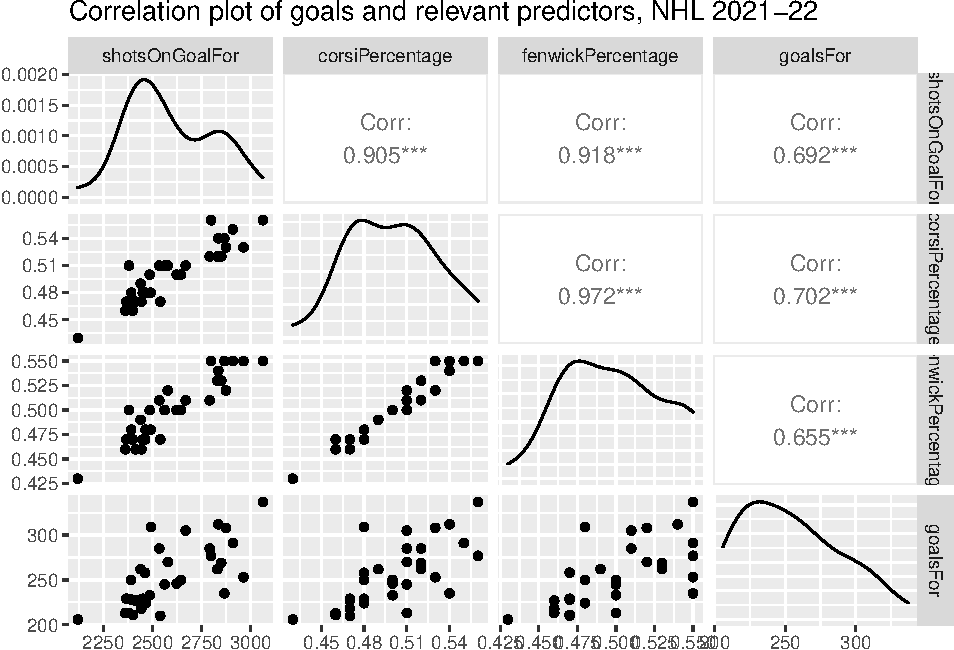
\includegraphics{textbook_files/figure-latex/unnamed-chunk-31-1.pdf}

Which quadrant of the graph represents goalies that faced a higher than average number of shots, but had a below-average save percentage?

\hfill\break
\hfill\break
\hfill\break

Which quadrant represents goalies that had a high save percentage and faced a high volume of shots?

\hfill\break
\hfill\break
\hfill\break

\hypertarget{correlation-plots}{%
\subsection{Correlation Plots}\label{correlation-plots}}

When analyzing sports data, there may be many circumstances where statisticians consider which of several variables are most highly correlated to an outcome variable of interest. In this case, it can be useful to use a correlation plot (also known as a correlation matrix or correlogram). Tidyverse and related packages provide many options for creating correlation plots.

Suppose a statistician has recently learned about some advanced hockey statistics and is interested in researching which stat has the highest correlation with goals scored. The statistician wants to compare team shots on goal, CORSI, and Fenwick to observe the association with goals scored for NHL teams.

\begin{example}
The following plot uses the same 2021-2022 data from Moneypuck.com; it gives the pairwise scatterplots and correlation values for each of the variables, as well as smoothed plots of each individual variable along the diagonals.
\end{example}

\begin{Shaded}
\begin{Highlighting}[]
\NormalTok{goal\_stats }\OtherTok{\textless{}{-}}\NormalTok{ nhl\_data\_all }\SpecialCharTok{\%\textgreater{}\%} 
  \FunctionTok{select}\NormalTok{(shotsOnGoalFor, corsiPercentage, fenwickPercentage, goalsFor)}
\FunctionTok{ggpairs}\NormalTok{(goal\_stats, }
        \AttributeTok{title=}\StringTok{"Correlation plot of goals and relevant predictors, NHL 2021{-}22"}\NormalTok{)}
\end{Highlighting}
\end{Shaded}

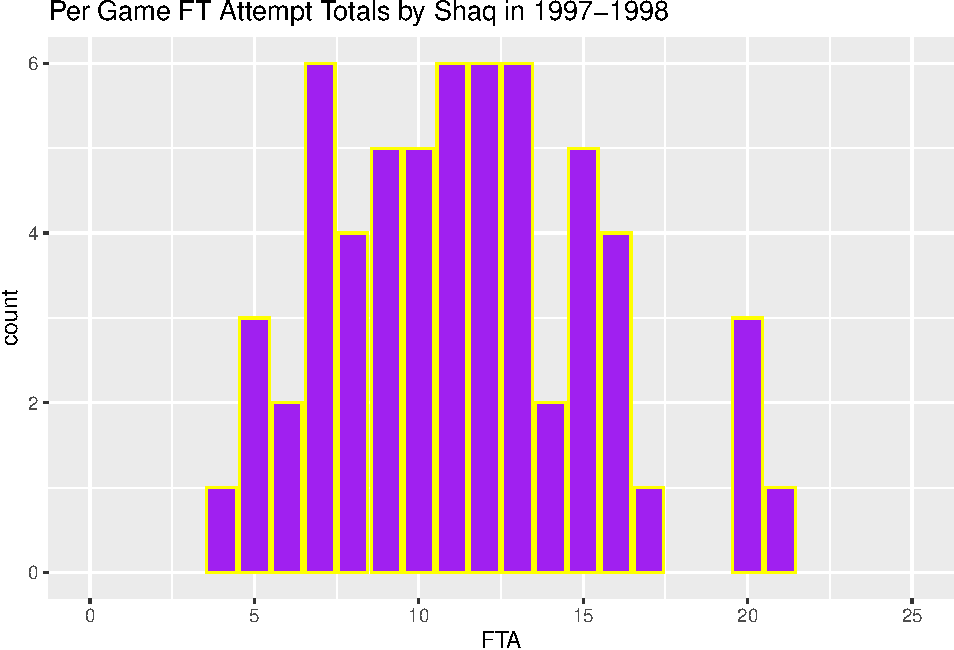
\includegraphics{textbook_files/figure-latex/unnamed-chunk-32-1.pdf}

Which of the variables has the strongest correlation with goals scored?\\
\strut \\
\strut \\
\strut \\
\strut \\

In the article \href{https://theathletic.com/121980/2017/10/09/an-advanced-stat-primer-understanding-basic-hockey-metrics/}{``An advanced stat primer: Understanding basic hockey metrics''}, Charlie O'Connor states, ``Generally speaking, Corsi is more predictive of future goal differential than Fenwick\ldots{} however, Fenwick forms the basis for the most widely-used Expected Goals models.'' Let's use the same predictors in a correlation plot with Expected Goals percentage. Does Fenwick have the strongest correlation with xGoal percentage?

\begin{Shaded}
\begin{Highlighting}[]
\NormalTok{xGoal\_stats }\OtherTok{\textless{}{-}}\NormalTok{ nhl\_data\_all }\SpecialCharTok{\%\textgreater{}\%} 
  \FunctionTok{select}\NormalTok{(shotsOnGoalFor, corsiPercentage, fenwickPercentage, xGoalsPercentage)}
\FunctionTok{ggpairs}\NormalTok{(xGoal\_stats,}
        \AttributeTok{title=}\StringTok{"Correlation plot of expected goals and relevant predictors, NHL 2021{-}22"}\NormalTok{)}
\end{Highlighting}
\end{Shaded}

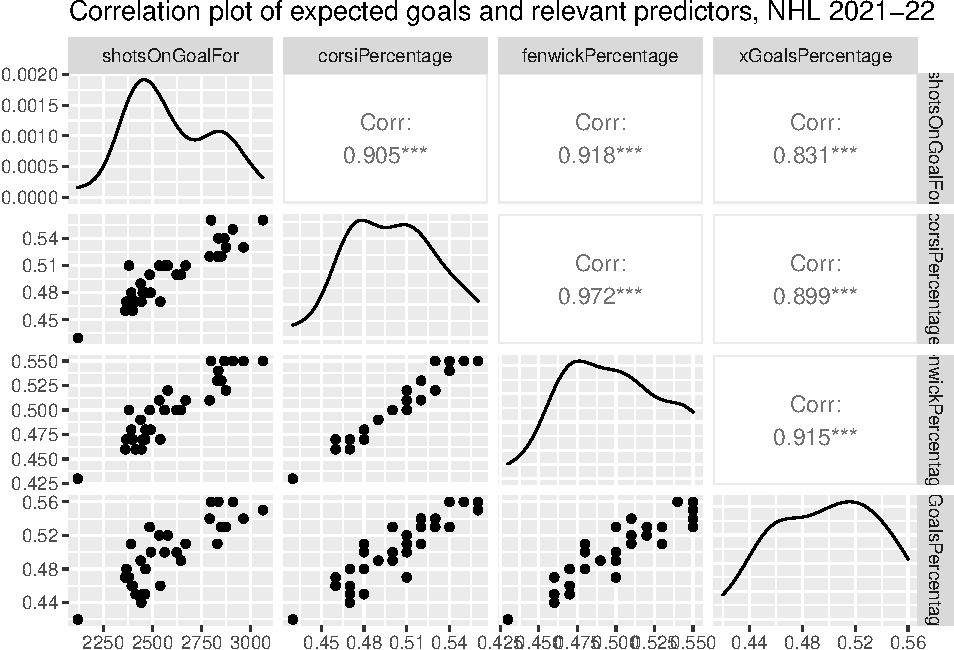
\includegraphics{textbook_files/figure-latex/hockey ggplot 6-1.pdf}

\newpage

\hypertarget{volleyball}{%
\section{Volleyball}\label{volleyball}}

Volleyball rules Youtube video: \url{https://www.youtube.com/watch?v=9g7nYQv-kPM}

\hypertarget{basic-volleyball-statistics}{%
\subsection{Basic Volleyball Statistics}\label{basic-volleyball-statistics}}

\begin{itemize}
\tightlist
\item
  A \textbf{Service Ace (SA)} occurs when a player's serve touches the ground on the other team's side without being touched by a player on that side.
\item
  A \textbf{Kill (K)} occurs when a player gets the ball over the net without it being returned by the opponent.
\item
  An \textbf{Assist (AST)} is a pass made directly before a player makes a kill.
\item
  \textbf{Hitting Percentage (PCT)} is the number of attempted kills (minus errors) divided by the total number of kill attempts. This helps determine how well a player or team is succeeding at their kill attempts.
\item
  A \textbf{Dig} is a pass of a hard-driven ball from the other team.
\end{itemize}

\emph{Reference:}\\
www.rookieroad.com

For Volleyball EDA, we will be using CSU Women's Volleyball data from the last five seasons.

\begin{Shaded}
\begin{Highlighting}[]
\CommentTok{\# Load CSU Women\textquotesingle{}s Volleyball Data}
\NormalTok{csu\_vb }\OtherTok{\textless{}{-}} \FunctionTok{read\_csv}\NormalTok{(}\StringTok{"data/csu\_volleyball.csv"}\NormalTok{)}
\FunctionTok{colnames}\NormalTok{(csu\_vb)[}\DecValTok{3}\NormalTok{] }\OtherTok{\textless{}{-}} \StringTok{"W\_L"}
\NormalTok{csu\_vb }\SpecialCharTok{\%\textgreater{}\%} \FunctionTok{slice\_head}\NormalTok{(}\AttributeTok{n=}\DecValTok{10}\NormalTok{) }\SpecialCharTok{\%\textgreater{}\%} \FunctionTok{select}\NormalTok{(}\DecValTok{1}\SpecialCharTok{:}\DecValTok{13}\NormalTok{) }\SpecialCharTok{\%\textgreater{}\%} \FunctionTok{kt}\NormalTok{()}
\end{Highlighting}
\end{Shaded}

\begin{table}[H]
\centering
\begin{tabular}{lllrrrrrrrrrr}
\toprule
Date & Opponent & W\_L & SP & K & E & TA & PCT & AST & SA & SE & RE & DIG\\
\midrule
8/25/17 & Duke & L & 5 & 66 & 28 & 179 & 0.212 & 64 & 5 & 13 & 6 & 84\\
8/26/17 & Central Florida & W & 4 & 56 & 18 & 126 & 0.302 & 52 & 7 & 10 & 7 & 49\\
8/29/17 & Northern Colorado & W & 3 & 39 & 8 & 77 & 0.403 & 38 & 5 & 12 & 4 & 29\\
9/1/17 & vs TCU & W & 5 & 62 & 20 & 149 & 0.282 & 59 & 6 & 10 & 7 & 65\\
9/1/17 & vs UNC Asheville & W & 3 & 41 & 7 & 80 & 0.425 & 39 & 8 & 8 & 5 & 28\\
9/2/17 & at Florida State & W & 3 & 48 & 12 & 95 & 0.379 & 45 & 6 & 4 & 1 & 42\\
9/8/17 & Ball State & W & 4 & 59 & 24 & 145 & 0.241 & 56 & 6 & 8 & 3 & 44\\
9/8/17 & Michigan & W & 3 & 48 & 8 & 101 & 0.396 & 46 & 3 & 6 & 4 & 37\\
9/10/17 & Idaho State & W & 3 & 46 & 11 & 92 & 0.380 & 46 & 4 & 3 & 4 & 48\\
9/15/17 & UAlbany & W & 3 & 41 & 7 & 73 & 0.466 & 36 & 5 & 5 & 1 & 30\\
\bottomrule
\end{tabular}
\end{table}

Let's look at a scatter plot of hitting percentage and the number of digs. While no conclusions can be drawn from such a plot, it can give us some insight into relationships worthy of further analysis. Before creating the plot using the code below, think about what you might expect the outcome to be.

\newpage

\hypertarget{scatter-plot}{%
\subsection{Scatter Plot}\label{scatter-plot}}

\begin{Shaded}
\begin{Highlighting}[]
\CommentTok{\# Digs, Hitting Percentage, Win/Lose}
\NormalTok{dig\_pct\_viz }\OtherTok{\textless{}{-}} \FunctionTok{ggplot}\NormalTok{(}\AttributeTok{data =}\NormalTok{ csu\_vb, }\FunctionTok{aes}\NormalTok{(}\AttributeTok{x =}\NormalTok{ DIG, }\AttributeTok{y =}\NormalTok{ PCT, }\AttributeTok{color =}\NormalTok{ W\_L)) }\SpecialCharTok{+}
  \FunctionTok{geom\_point}\NormalTok{()}
\NormalTok{dig\_pct\_viz}
\end{Highlighting}
\end{Shaded}

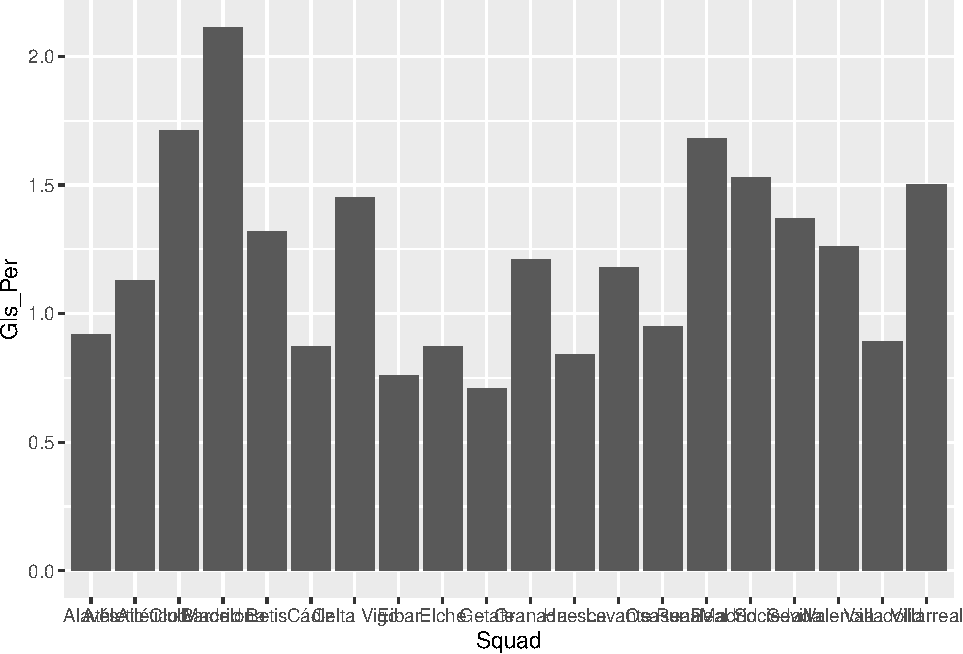
\includegraphics{textbook_files/figure-latex/unnamed-chunk-34-1.pdf}
\newpage

Let's change the axis titles, legend title, and add a main title.

\begin{Shaded}
\begin{Highlighting}[]
\NormalTok{dig\_pct\_viz }\SpecialCharTok{+}
  \FunctionTok{labs}\NormalTok{(}\AttributeTok{title =} \StringTok{"Wins and Losses by Number of Digs and Hitting Percentage"}\NormalTok{,}
       \AttributeTok{x =} \StringTok{"Number of Digs (DIG)"}\NormalTok{, }\AttributeTok{y =} \StringTok{"Hitting Percentage (PCT)"}\NormalTok{,}
       \AttributeTok{color =} \StringTok{"Win or Loss"}\NormalTok{)}
\end{Highlighting}
\end{Shaded}

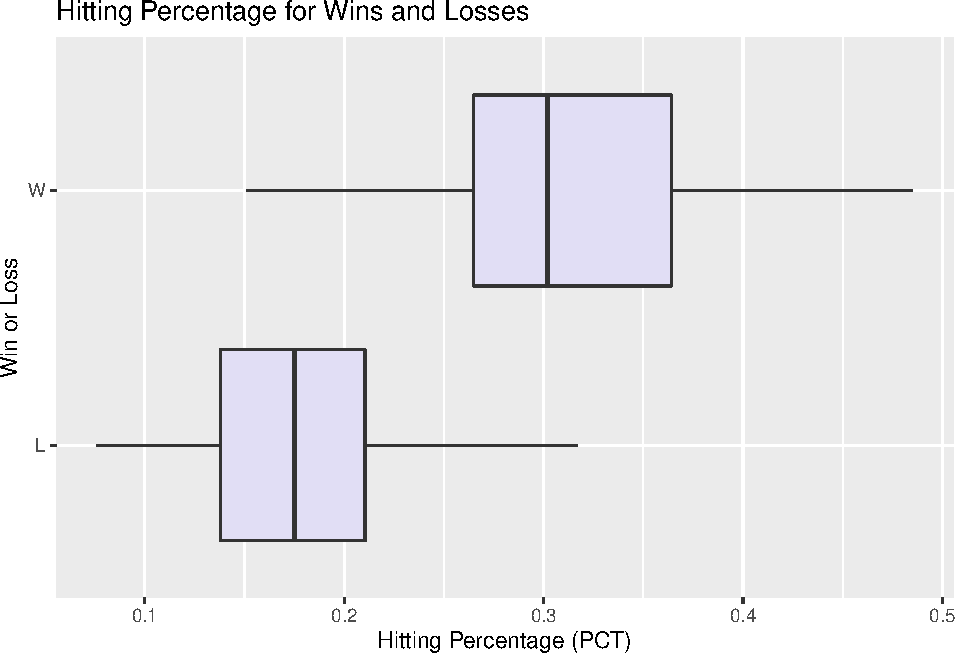
\includegraphics{textbook_files/figure-latex/unnamed-chunk-35-1.pdf}

What can we learn from this visual? Well, we can see that there is a weak linear relationship between the number of digs and hitting percentage. To an extent, hitting percentage decreases as the number of digs increases. Why is this the case? Maybe if a team has a really high hitting percentage, this means that the opposing team does not have as many opportunities to attack the other team offensively, reducing the number of opportunities for digs. It also seems that while wins and losses are somewhat evenly spread across the number of digs, there is a more clear cutoff for hitting percentage. It seems that the majority of wins are associated with a hitting percentage of at least 0.2, while the majority of losses are associated with a hitting percentage of less than 0.3.

\newpage

\hypertarget{box-plot}{%
\subsection{Box Plot}\label{box-plot}}

Now let's take a closer look at the distribution of hitting percentage and digs for wins and losses. To do this, we will create box plots for each statistic.

\begin{Shaded}
\begin{Highlighting}[]
\NormalTok{pct\_viz }\OtherTok{\textless{}{-}} \FunctionTok{ggplot}\NormalTok{(}\AttributeTok{data =}\NormalTok{ csu\_vb, }\FunctionTok{aes}\NormalTok{(}\AttributeTok{x =}\NormalTok{ PCT, }\AttributeTok{y =}\NormalTok{ W\_L)) }\SpecialCharTok{+}
  \FunctionTok{geom\_boxplot}\NormalTok{()}
\NormalTok{pct\_viz}
\end{Highlighting}
\end{Shaded}

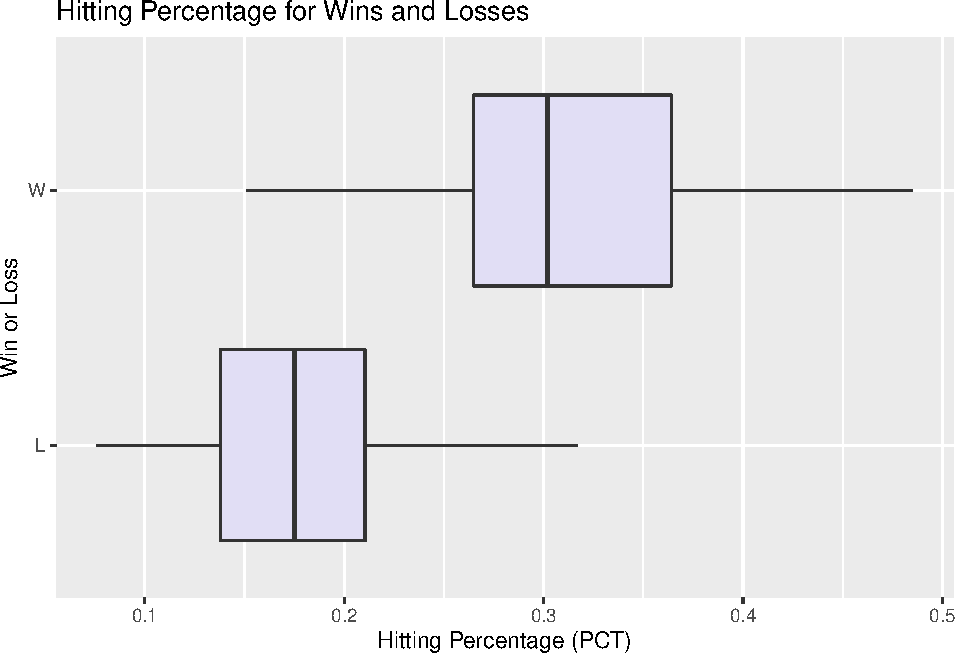
\includegraphics{textbook_files/figure-latex/unnamed-chunk-36-1.pdf}

\begin{Shaded}
\begin{Highlighting}[]
\NormalTok{dig\_viz }\OtherTok{\textless{}{-}} \FunctionTok{ggplot}\NormalTok{(}\AttributeTok{data =}\NormalTok{ csu\_vb, }\FunctionTok{aes}\NormalTok{(}\AttributeTok{x =}\NormalTok{ DIG, }\AttributeTok{y =}\NormalTok{ W\_L)) }\SpecialCharTok{+}
  \FunctionTok{geom\_boxplot}\NormalTok{()}
\NormalTok{dig\_viz}
\end{Highlighting}
\end{Shaded}

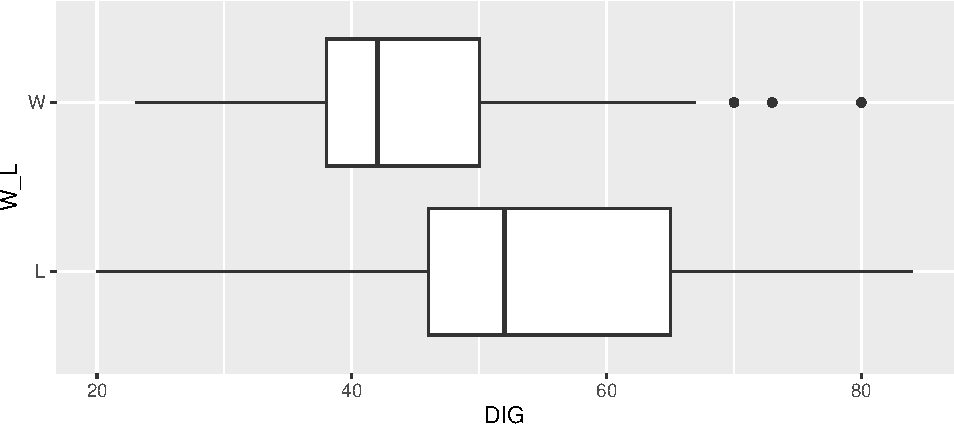
\includegraphics{textbook_files/figure-latex/unnamed-chunk-36-2.pdf}
\newpage

Let's modify these plots to make them more complete and visually appealing.

\begin{Shaded}
\begin{Highlighting}[]
\NormalTok{pct\_viz }\SpecialCharTok{+}
  \FunctionTok{labs}\NormalTok{(}\AttributeTok{title =} \StringTok{"Hitting Percentage for Wins and Losses"}\NormalTok{,}
       \AttributeTok{x =} \StringTok{"Hitting Percentage (PCT)"}\NormalTok{,}
       \AttributeTok{y =} \StringTok{"Win or Loss"}\NormalTok{) }\SpecialCharTok{+}
  \FunctionTok{geom\_boxplot}\NormalTok{(}\AttributeTok{fill =} \StringTok{"slateblue"}\NormalTok{, }\AttributeTok{alpha =} \FloatTok{0.2}\NormalTok{)}
\end{Highlighting}
\end{Shaded}

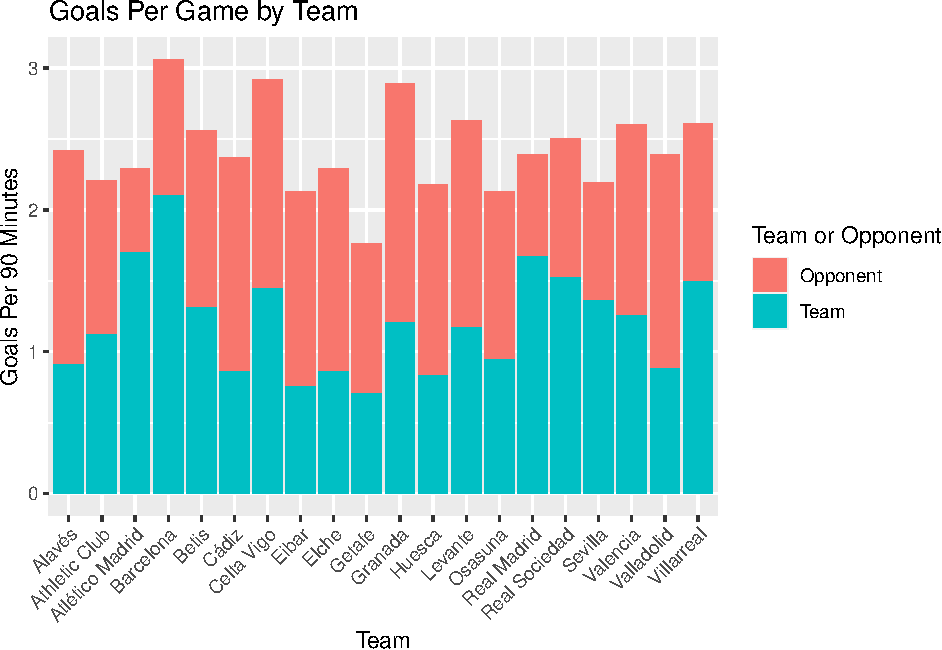
\includegraphics{textbook_files/figure-latex/unnamed-chunk-37-1.pdf}

\begin{Shaded}
\begin{Highlighting}[]
\NormalTok{dig\_viz }\SpecialCharTok{+}
  \FunctionTok{labs}\NormalTok{(}\AttributeTok{title =} \StringTok{"Number of Digs for Wins and Losses"}\NormalTok{,}
       \AttributeTok{x =} \StringTok{"Number of Digs (DIG)"}\NormalTok{,}
       \AttributeTok{y =} \StringTok{"Win or Loss"}\NormalTok{) }\SpecialCharTok{+}
  \FunctionTok{geom\_boxplot}\NormalTok{(}\AttributeTok{fill =} \StringTok{"slateblue"}\NormalTok{, }\AttributeTok{alpha =} \FloatTok{0.2}\NormalTok{)}
\end{Highlighting}
\end{Shaded}

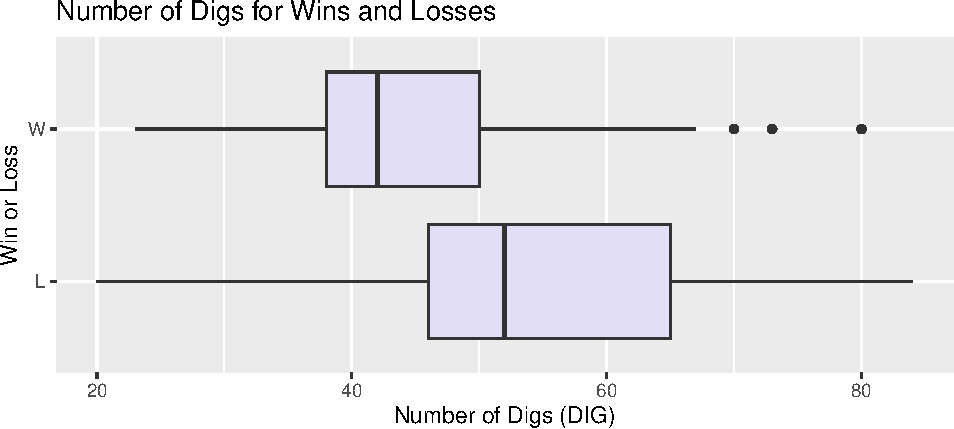
\includegraphics{textbook_files/figure-latex/unnamed-chunk-37-2.pdf}

Box plots allow us to isolate each statistic (number of kills and hitting percentage) so we can more clearly determine the center and spread of each between wins and losses.

\newpage

\hypertarget{soccer}{%
\section{Soccer}\label{soccer}}

Rules of Soccer YouTube video: \url{https://www.youtube.com/watch?v=dFLaabgXhpc}

\hypertarget{basic-soccer-statistics}{%
\subsection{Basic Soccer Statistics}\label{basic-soccer-statistics}}

\begin{itemize}
\item
  \textbf{Shots (SH)} represent all shots taken by a team throughout the game. This is simply an attempt by a player to shoot the ball toward the net, even if they miss or the shot is saved (Rookie Road).
\item
  \textbf{Shots on Goal (SOG)} represent all shots that would have gone into the goal if not saved by a defender or goalkeeper (Rookie Road).
\item
  \textbf{Assist (A)} occur when a player passes the ball to someone, and the next shot results in a goal.
\item
  \textbf{Possession} refers to the percentage of time a team had control of the ball during a game.
\end{itemize}

\hypertarget{advanced-soccer-statistics}{%
\subsection{Advanced Soccer Statistics}\label{advanced-soccer-statistics}}

\begin{itemize}
\tightlist
\item
  \textbf{Expected Goals (xG)} ``indicates how many goals a team could have expected to score based on the quantity and quality of chances that they created in a match'' (Tippett 2019, 4).
\end{itemize}

These definitions come from www.rookieroad.com and ``The Expected Goals Philosophy'' by James Tippett.

To learn more about expected goals, check out this YouTube video:\\
\url{https://www.youtube.com/watch?v=w7zPZsLGK18}

\newpage

\hypertarget{bar-plot}{%
\subsection{Bar Plot}\label{bar-plot}}

Now that we have an understanding of some basic shooting statistics, let us go through some EDA examples. For this first example, we will need to install the ``worldfootballR'' package.

\begin{Shaded}
\begin{Highlighting}[]
\FunctionTok{library}\NormalTok{(worldfootballR)}
\end{Highlighting}
\end{Shaded}

Next we will look at some data specific to La Liga, which is a soccer league in the men's top professional soccer division.

\begin{Shaded}
\begin{Highlighting}[]
\CommentTok{\# Get "Squad Standard Stats" Data}
\NormalTok{big5\_2021\_stats }\OtherTok{\textless{}{-}} \FunctionTok{fb\_big5\_advanced\_season\_stats}\NormalTok{(}
  \AttributeTok{season\_end\_year =} \DecValTok{2021}\NormalTok{, }\AttributeTok{stat\_type =} \StringTok{"standard"}\NormalTok{, }\AttributeTok{team\_or\_player =} \StringTok{"team"}\NormalTok{)}
\NormalTok{liga\_2021\_stats }\OtherTok{\textless{}{-}}\NormalTok{ big5\_2021\_stats[}\FunctionTok{which}\NormalTok{((big5\_2021\_stats}\SpecialCharTok{$}\NormalTok{Comp }\SpecialCharTok{==} \StringTok{"La Liga"}\NormalTok{)),]}

\CommentTok{\# look at the first ten entries and a selection of columns}
\NormalTok{liga\_2021\_stats }\SpecialCharTok{\%\textgreater{}\%} 
  \FunctionTok{select}\NormalTok{(Squad,Team\_or\_Opponent,Poss,Gls,Ast,xG\_Expected,xA\_Expected) }\SpecialCharTok{\%\textgreater{}\%} 
  \FunctionTok{slice\_head}\NormalTok{(}\AttributeTok{n=}\DecValTok{10}\NormalTok{) }\SpecialCharTok{\%\textgreater{}\%} \FunctionTok{kt}\NormalTok{()}
\end{Highlighting}
\end{Shaded}

\begin{Shaded}
\begin{Highlighting}[]
\CommentTok{\# Create visual for each team\textquotesingle{}s goals per game}
\NormalTok{team\_goals\_viz }\OtherTok{\textless{}{-}} 
  \FunctionTok{ggplot}\NormalTok{(}\AttributeTok{data =}\NormalTok{ liga\_2021\_stats[}\FunctionTok{which}\NormalTok{(liga\_2021\_stats}\SpecialCharTok{$}\NormalTok{Team\_or\_Opponent }\SpecialCharTok{==} \StringTok{"team"}\NormalTok{),], }
                         \FunctionTok{aes}\NormalTok{(}\AttributeTok{x =}\NormalTok{ Squad, }\AttributeTok{y =}\NormalTok{ Gls\_Per)) }\SpecialCharTok{+}
  \FunctionTok{theme}\NormalTok{(}\AttributeTok{axis.text.x =} \FunctionTok{element\_text}\NormalTok{(}\AttributeTok{angle =} \DecValTok{45}\NormalTok{, }\AttributeTok{hjust =} \DecValTok{1}\NormalTok{)) }\SpecialCharTok{+}
  \FunctionTok{geom\_bar}\NormalTok{(}\AttributeTok{stat =} \StringTok{"identity"}\NormalTok{)}
\NormalTok{team\_goals\_viz}
\end{Highlighting}
\end{Shaded}

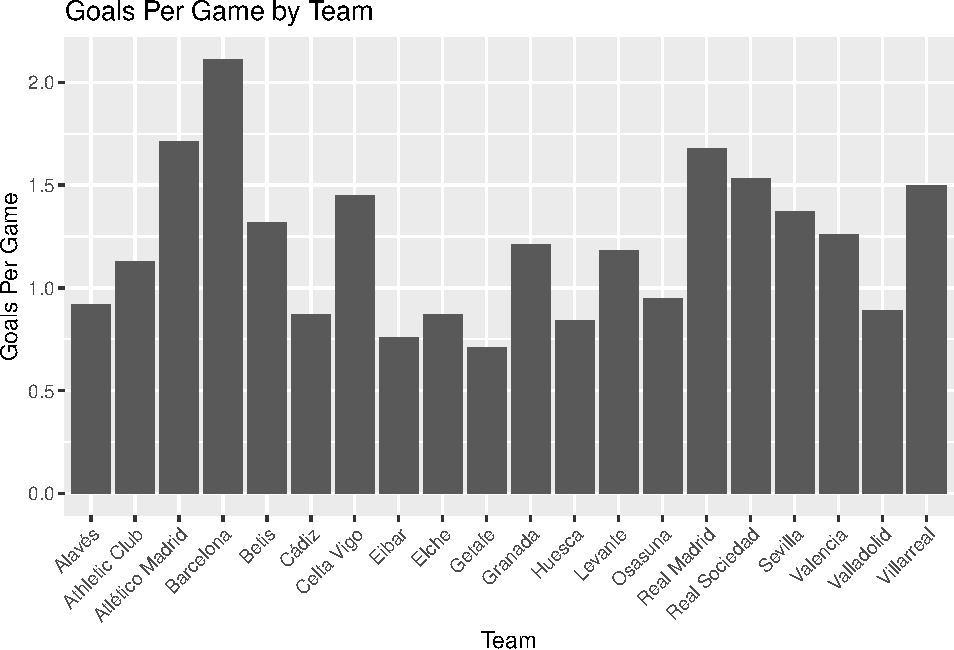
\includegraphics{textbook_files/figure-latex/unnamed-chunk-41-1.pdf}

\newpage

This plot is a good starting point, but still looks pretty messy. Let's add a title, change the axis titles, and rotate the axis labels so they are not overlapping over one another.

\begin{Shaded}
\begin{Highlighting}[]
\NormalTok{team\_goals\_viz }\OtherTok{\textless{}{-}}\NormalTok{ team\_goals\_viz }\SpecialCharTok{+}
  \FunctionTok{xlab}\NormalTok{(}\StringTok{"Team"}\NormalTok{) }\SpecialCharTok{+}
  \FunctionTok{ylab}\NormalTok{(}\StringTok{"Goals Per Game"}\NormalTok{) }\SpecialCharTok{+}
  \FunctionTok{theme}\NormalTok{(}\AttributeTok{axis.text.x =} \FunctionTok{element\_text}\NormalTok{(}\AttributeTok{angle =} \DecValTok{45}\NormalTok{, }\AttributeTok{hjust =} \DecValTok{1}\NormalTok{)) }\SpecialCharTok{+}
  \FunctionTok{ggtitle}\NormalTok{(}\StringTok{"Goals Per Game by Team"}\NormalTok{)}
\NormalTok{team\_goals\_viz}
\end{Highlighting}
\end{Shaded}

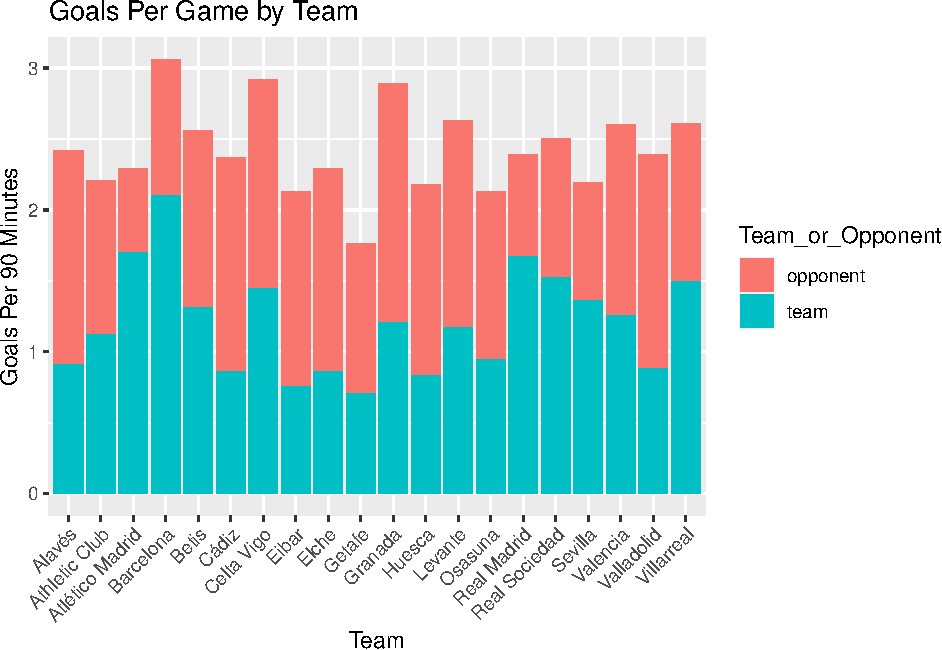
\includegraphics{textbook_files/figure-latex/unnamed-chunk-42-1.pdf}

\newpage

This is already looking a lot better. Now, we will add the goals scored per game \emph{against} each team. Why is this of interest? Well, at first glance, Barcelona seems like a pretty impressive team, as they score more goals per game than any other team in the league. However, what if they also have more goals scored against them than any other team in the league? This could be important context, so we will include it in the graph below.

\begin{Shaded}
\begin{Highlighting}[]
\NormalTok{all\_goals\_viz }\OtherTok{\textless{}{-}} \FunctionTok{ggplot}\NormalTok{(}\AttributeTok{data =}\NormalTok{ liga\_2021\_stats, }\FunctionTok{aes}\NormalTok{(}\AttributeTok{x =}\NormalTok{ Squad, }\AttributeTok{y =}\NormalTok{ Gls\_Per)) }\SpecialCharTok{+}
  \FunctionTok{geom\_bar}\NormalTok{(}\AttributeTok{stat =} \StringTok{"identity"}\NormalTok{, }\FunctionTok{aes}\NormalTok{(}\AttributeTok{fill =}\NormalTok{ Team\_or\_Opponent), }\AttributeTok{position =} \StringTok{"stack"}\NormalTok{) }\SpecialCharTok{+}
  \FunctionTok{xlab}\NormalTok{(}\StringTok{"Team"}\NormalTok{) }\SpecialCharTok{+}
  \FunctionTok{ylab}\NormalTok{(}\StringTok{"Goals Per 90 Minutes"}\NormalTok{) }\SpecialCharTok{+}
  \FunctionTok{theme}\NormalTok{(}\AttributeTok{axis.text.x =} \FunctionTok{element\_text}\NormalTok{(}\AttributeTok{angle =} \DecValTok{45}\NormalTok{, }\AttributeTok{hjust =} \DecValTok{1}\NormalTok{)) }\SpecialCharTok{+}
  \FunctionTok{ggtitle}\NormalTok{(}\StringTok{"Goals Per Game by Team"}\NormalTok{)}
\NormalTok{all\_goals\_viz}
\end{Highlighting}
\end{Shaded}

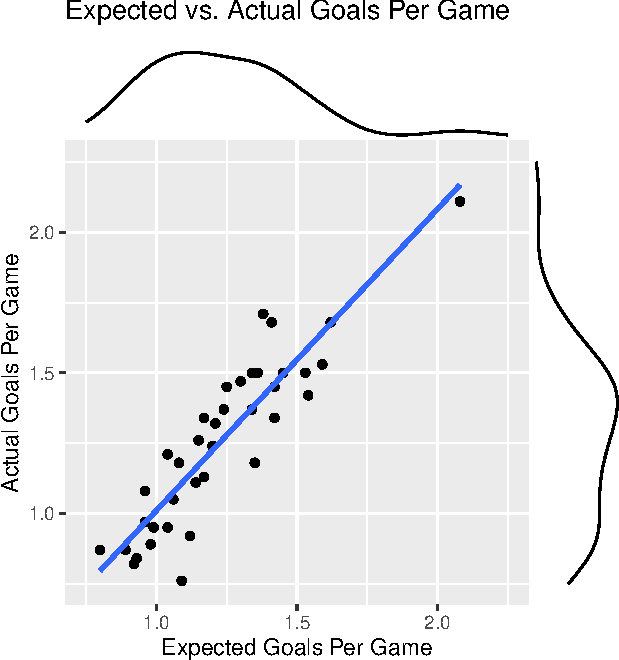
\includegraphics{textbook_files/figure-latex/unnamed-chunk-43-1.pdf}

\newpage

This is looking pretty good, but let's clean it up just a bit by changing the legend title and labels.

\begin{Shaded}
\begin{Highlighting}[]
\NormalTok{all\_goals\_viz }\SpecialCharTok{+}
  \FunctionTok{scale\_fill\_discrete}\NormalTok{(}\AttributeTok{name =} \StringTok{"Team or Opponent"}\NormalTok{, }\AttributeTok{labels =} \FunctionTok{c}\NormalTok{(}\StringTok{"Opponent"}\NormalTok{,}\StringTok{"Team"}\NormalTok{))}
\end{Highlighting}
\end{Shaded}

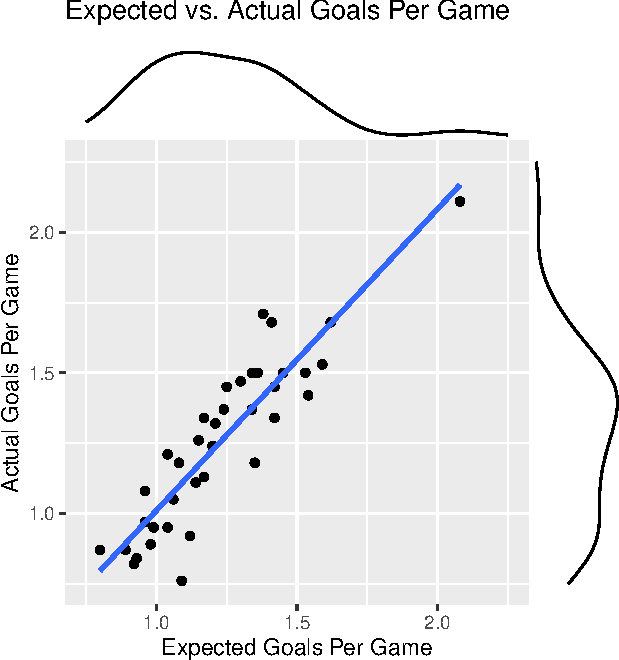
\includegraphics{textbook_files/figure-latex/unnamed-chunk-44-1.pdf}

What does this graph show us? Well, we are able to see the average number of goals scored for and against each team per game. It looks like Barcelona is scoring a lot more goals than they are letting be scored against them, while other teams like Valladolid tend to have a higher proportion of goals scored for the opposing team.

\newpage

\hypertarget{scatter-plot-1}{%
\subsection{Scatter Plot}\label{scatter-plot-1}}

In addition to simply knowing the average actual number of goals scored for and against each team per game, we may be interested in how this compares to the expected number of goals scored per game, as well.

\begin{Shaded}
\begin{Highlighting}[]
\FunctionTok{library}\NormalTok{(ggExtra)}
\NormalTok{act\_exp\_viz }\OtherTok{\textless{}{-}} \FunctionTok{ggplot}\NormalTok{(}\AttributeTok{data =}\NormalTok{ liga\_2021\_stats, }
                      \FunctionTok{aes}\NormalTok{(}\AttributeTok{x =}\NormalTok{ xG\_Per, }\AttributeTok{y =}\NormalTok{ Gls\_Per, }\AttributeTok{label =}\NormalTok{ Squad)) }\SpecialCharTok{+}
  \FunctionTok{geom\_point}\NormalTok{() }\SpecialCharTok{+}
  \FunctionTok{scale\_x\_continuous}\NormalTok{(}\AttributeTok{limits =} \FunctionTok{c}\NormalTok{(}\FloatTok{0.75}\NormalTok{,}\FloatTok{2.25}\NormalTok{)) }\SpecialCharTok{+}
  \FunctionTok{scale\_y\_continuous}\NormalTok{(}\AttributeTok{limits =} \FunctionTok{c}\NormalTok{(}\FloatTok{0.75}\NormalTok{,}\FloatTok{2.25}\NormalTok{)) }\SpecialCharTok{+}
  \FunctionTok{ggtitle}\NormalTok{(}\StringTok{"Expected vs. Actual Goals Per Game"}\NormalTok{) }\SpecialCharTok{+}
  \FunctionTok{xlab}\NormalTok{(}\StringTok{"Expected Goals Per Game"}\NormalTok{) }\SpecialCharTok{+}
  \FunctionTok{ylab}\NormalTok{(}\StringTok{"Actual Goals Per Game"}\NormalTok{) }\SpecialCharTok{+}
  \FunctionTok{geom\_smooth}\NormalTok{(}\AttributeTok{method =} \StringTok{"lm"}\NormalTok{, }\AttributeTok{se =} \ConstantTok{FALSE}\NormalTok{) }\SpecialCharTok{+}
  \FunctionTok{theme}\NormalTok{(}\AttributeTok{aspect.ratio =} \DecValTok{2}\SpecialCharTok{/}\DecValTok{2}\NormalTok{)}
\FunctionTok{ggMarginal}\NormalTok{(act\_exp\_viz, }\AttributeTok{type =} \StringTok{"density"}\NormalTok{)}
\end{Highlighting}
\end{Shaded}

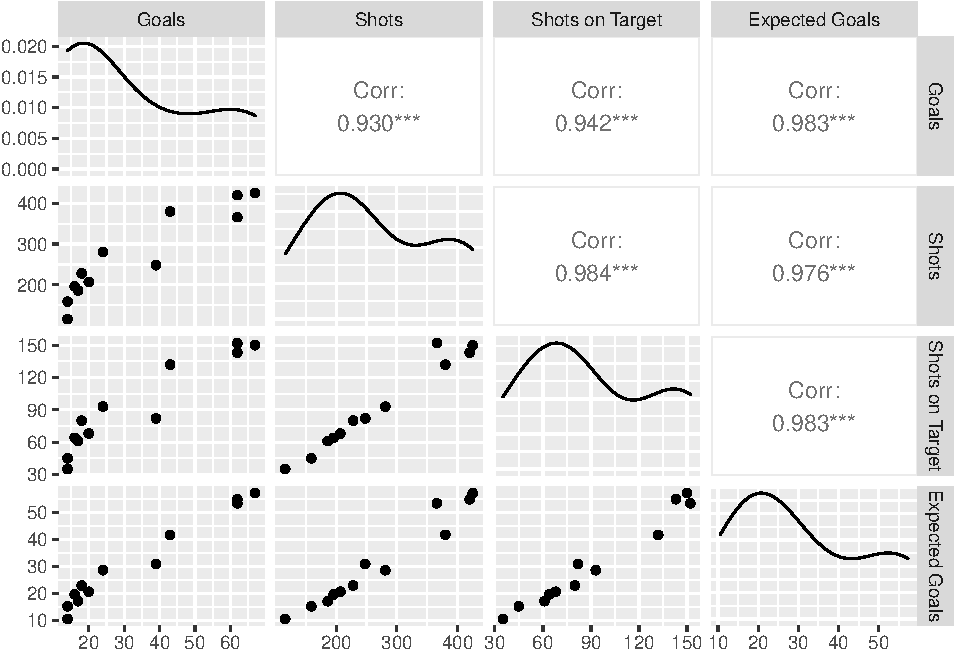
\includegraphics{textbook_files/figure-latex/unnamed-chunk-45-1.pdf}

As you can see, we fit a line to the data. At first glance, it seems to have a positive slope slightly greater than 1. What does this mean in the scenario of actual and expected goals per game?

\newpage

\begin{example}
Use the \texttt{worldfootballR} package to collect team shooting data from the Women's 1st Tier League (Women's Super League) in England for 2020-2021. Plot goals vs.~shots, shots on target, and expected goals. Comment on the relationships.
\end{example}

\begin{Shaded}
\begin{Highlighting}[]
\NormalTok{wsl\_2021\_shooting }\OtherTok{\textless{}{-}} \FunctionTok{get\_season\_team\_stats}\NormalTok{(}
  \AttributeTok{country =} \StringTok{"ENG"}\NormalTok{, }\AttributeTok{gender =} \StringTok{"F"}\NormalTok{, }\AttributeTok{season\_end\_year =} \StringTok{"2021"}\NormalTok{, }
  \AttributeTok{tier =} \StringTok{"1st"}\NormalTok{, }\AttributeTok{stat\_type =} \StringTok{"shooting"}\NormalTok{)}
\end{Highlighting}
\end{Shaded}

\begin{verbatim}
## Warning: 'get_season_team_stats' is deprecated.
## Use 'fb_season_team_stats' instead.
## See help("Deprecated")
\end{verbatim}

\begin{Shaded}
\begin{Highlighting}[]
\NormalTok{wsl\_2021\_shooting }\OtherTok{\textless{}{-}}\NormalTok{wsl\_2021\_shooting }\SpecialCharTok{\%\textgreater{}\%} 
  \FunctionTok{select}\NormalTok{(Squad,Gls\_Standard,Sh\_Standard,SoT\_Standard,xG\_Expected) }\SpecialCharTok{\%\textgreater{}\%} 
  \FunctionTok{rename}\NormalTok{(}\AttributeTok{Goals=}\NormalTok{Gls\_Standard,}\AttributeTok{Shots=}\NormalTok{Sh\_Standard,}
         \StringTok{\textasciigrave{}}\AttributeTok{Shots on Target}\StringTok{\textasciigrave{}}\OtherTok{=}\NormalTok{SoT\_Standard,}\StringTok{\textasciigrave{}}\AttributeTok{Expected Goals}\StringTok{\textasciigrave{}} \OtherTok{=}\NormalTok{ xG\_Expected)}
\NormalTok{wsl\_2021\_shooting }\SpecialCharTok{\%\textgreater{}\%} \FunctionTok{kt}\NormalTok{()}
\end{Highlighting}
\end{Shaded}

\begin{table}[H]
\centering
\begin{tabular}{lrrrr}
\toprule
Squad & Goals & Shots & Shots on Target & Expected Goals\\
\midrule
Arsenal & 62 & 374 & 152 & 48.2\\
Aston Villa & 14 & 156 & 46 & 13.5\\
Birmingham City & 14 & 97 & 34 & 10.6\\
Brighton & 20 & 196 & 71 & 17.8\\
Bristol City & 17 & 186 & 58 & 15.4\\
Chelsea & 68 & 418 & 151 & 53.6\\
Everton & 39 & 245 & 82 & 29.4\\
Manchester City & 62 & 426 & 143 & 54.1\\
Manchester Utd & 43 & 364 & 126 & 38.9\\
Reading & 24 & 283 & 95 & 26.0\\
Tottenham & 16 & 187 & 63 & 16.5\\
West Ham & 18 & 224 & 84 & 19.8\\
vs Arsenal & 14 & 165 & 51 & 14.5\\
vs Aston Villa & 45 & 362 & 129 & 35.3\\
vs Birmingham City & 43 & 363 & 127 & 35.0\\
vs Brighton & 41 & 304 & 89 & 35.8\\
vs Bristol City & 68 & 417 & 162 & 49.7\\
vs Chelsea & 9 & 132 & 36 & 12.7\\
vs Everton & 29 & 233 & 81 & 27.1\\
vs Manchester City & 13 & 124 & 41 & 11.0\\
vs Manchester Utd & 17 & 203 & 69 & 18.8\\
vs Reading & 41 & 281 & 104 & 33.3\\
vs Tottenham & 40 & 279 & 103 & 32.5\\
vs West Ham & 37 & 293 & 113 & 38.2\\
\bottomrule
\end{tabular}
\end{table}

\newpage

\begin{Shaded}
\begin{Highlighting}[]
\NormalTok{wsl\_2021\_shooting }\OtherTok{\textless{}{-}}\NormalTok{ wsl\_2021\_shooting }\SpecialCharTok{\%\textgreater{}\%}
  \FunctionTok{slice\_head}\NormalTok{(}\AttributeTok{n=}\DecValTok{12}\NormalTok{)}
\NormalTok{wsl\_2021\_shooting }\SpecialCharTok{\%\textgreater{}\%} 
  \FunctionTok{select}\NormalTok{(Goals,Shots,}\StringTok{\textasciigrave{}}\AttributeTok{Shots on Target}\StringTok{\textasciigrave{}}\NormalTok{,}\StringTok{\textasciigrave{}}\AttributeTok{Expected Goals}\StringTok{\textasciigrave{}}\NormalTok{) }\SpecialCharTok{\%\textgreater{}\%} 
  \FunctionTok{ggpairs}\NormalTok{()}
\end{Highlighting}
\end{Shaded}

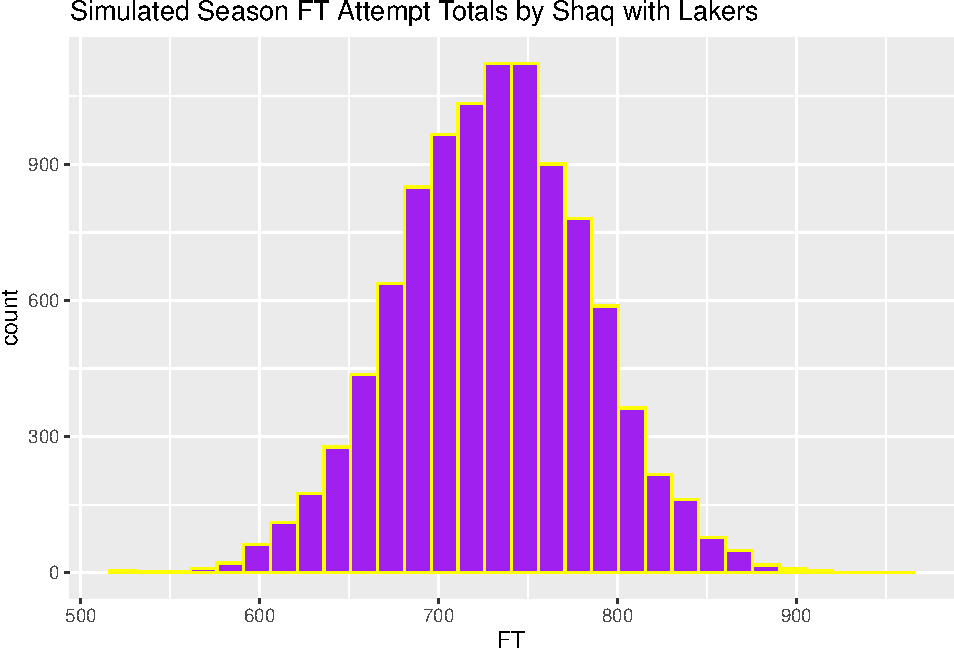
\includegraphics{textbook_files/figure-latex/unnamed-chunk-47-1.pdf}

\hypertarget{probability}{%
\chapter{Probability}\label{probability}}

\hypertarget{definitions-and-set-theory}{%
\section{Definitions and Set Theory}\label{definitions-and-set-theory}}

\begin{definition}
An \textbf{\emph{experiment}} is any activity or process whose outcome is subject to uncertainty.
\end{definition}

\begin{definition}
The \textbf{\emph{sample space}} of an experiment, denoted by \(\Omega\) or \(\mathcal{S}\), is the set of all possible outcomes of that experiment.
\end{definition}

\begin{definition}
An \textbf{\emph{event}} is any collection (subset) of outcomes contained in the sample space, \(\Omega\).
\end{definition}

\begin{example}
Give some examples of discrete random variables in sports.
\end{example}

\hfill\break
\hfill\break
\hfill\break
\hfill\break
\hfill\break

\begin{example}
Give some examples of continuous random variables in sports.
\end{example}

~\\
\strut \\
\strut \\
\strut \\

\newpage

For the following examples, suppose that we are interested in the batting outcomes of a plate appearance in baseball.

Let \(A\) be the event that the batter gets walked, let \(B\) be the event that the batter gets a hit, let \(C\) be the event that the batter strikes out, and let \(D\) be the event that the batter makes it to first base at the end of their at bat.

We will define a handful of set operations to help us when we begin calculating the probability of different events occurring.

\begin{definition}
The \textbf{\emph{compliment}} of an event \(A\), denoted by \(A^c\) or \(A'\), is the set of all outcomes in \(\Omega\) that are not contained in \(A\).
\end{definition}

\begin{example}
Draw a Venn diagram illustrating \(A^c\) and describe the event.
\end{example}

\hfill\break
\hfill\break
\hfill\break
\hfill\break
\hfill\break
\vfill

\begin{definition}
The \textbf{\emph{union}} of two events \(A\) and \(B\), denoted by \(A \cup B\) and read ``\(A\) or \(B\)'', is the event consisting of all outcomes that are either in \(A\) or \(B\) or in both.
\end{definition}

\begin{example}
Draw a Venn diagram illustrating \(A \cup D\) and describe the event.
\end{example}

\hfill\break
\hfill\break
\hfill\break
\hfill\break
\hfill\break
\vfill

\newpage

\begin{definition}
The \textbf{\emph{intersection}} of two events \(A\) and \(B\), denoted by \(A \cap B\) and read ``\(A\) and \(B\)'', is the event consisting of all outcomes that are in both \(A\) and \(B\).
\end{definition}

\begin{example}
Draw a Venn diagram illustrating \(A \cap D\) and describe the event.
\end{example}

\hfill\break
\hfill\break
\hfill\break
\hfill\break
\hfill\break
\vfill

\begin{definition}
The \textbf{\emph{difference}} of two events \(A\) and \(B\), denoted by \(A \mathbin{/} B\) and read ``difference of \(A\) and \(B\)'', is
the event consisting of all outcomes that are in \(A\) but not in \(B\).
\end{definition}

\begin{example}
Draw a Venn diagram illustrating \(D \mathbin{/} A\) and describe the event.
\end{example}

\hfill\break
\hfill\break
\hfill\break
\hfill\break
\hfill\break
\vfill

\begin{definition}
Two events \(A\) and \(B\) are said to be \textbf{\emph{disjoint}} (or \textbf{\emph{mutually exclusive}}) if \(A \cap B = \emptyset\)
\end{definition}

\begin{example}
Are the events \(A\) and \(B\) disjoint? How about \(A\) and \(D\)?
\end{example}

\hfill\break
\hfill\break
\hfill\break
\hfill\break
\hfill\break
\vfill

\newpage

\hypertarget{axioms-properties-and-laws}{%
\section{Axioms, Properties, and Laws}\label{axioms-properties-and-laws}}

There are some basic assumptions or ``axioms'' which are the foundation of the theory of probability. Andrey Kolmogorov first described these axioms in 1933.

\hypertarget{axioms-of-probability}{%
\subsection{Axioms of Probability}\label{axioms-of-probability}}

\begin{enumerate}
\def\labelenumi{\arabic{enumi}.}
\tightlist
\item
  \(P(A) \geq 0\), for any event \(A\)\\
\item
  \(P(\Omega) = 1\)\\
\item
  If \(A_1, A_2, A_3, \ldots\) is a collection of disjoint events, then:\\
  \(P(\cup_{i=1}^{\infty} A_i) = P(A_1 \cup A_2 \cup \ldots ) = \sum_{i=1}^{\infty} P(A_i)\)\\
\end{enumerate}

Note that all probabilities are between 0 and 1, that is, for any event \(A\), \(0 \leq P(A) \leq 1\).

We can convert to percentages by multiplying probabilities by 100, however, this is a set that is only done after all calculations have been completed.

\hypertarget{properties-of-probability}{%
\subsection{Properties of Probability}\label{properties-of-probability}}

\begin{itemize}
\item
  \(P(\emptyset) = 0\)\\
\item
  \(P(A^c) = 1 - P(A)\)\\
\item
  \(P(A \cup B) = P(A) + P(B) - P(A \cap B)\)\\
\item
  \(P(A \cup B \cup C) = \\ P(A) + P(B) + P(C) - P(A \cap B) - P(A \cap C) - P(B \cap C) + P(A \cap B \cap C)\)\\
\item
  \(P([A \cup B]^c) = P(A^c \cap B^c)\)\\
\item
  \(P([A \cap B]^c) = P(A^c \cup B^c)\)\\
\end{itemize}

\newpage

\begin{example}
In 2001, Barry Bonds broke the single season home run record with 73 home runs. In this season, he had 664 plate appearances (476 at-bats), 156 hits, 177 walks, 9 hit by pitches, and 2 sacrifice flies. Use this information to answer the following questions.
\end{example}

\begin{enumerate}
\def\labelenumi{(\alph{enumi})}
\item
  Plate appearances that result in a walk, hit by pitch, or sacrifice fly are not counted towards a player's at-bats. Confirm that Bonds had 476 official at-bats.\\
  \strut \\
  \strut \\
  \strut \\
  \vfill
\item
  Suppose an at-bat is chosen at random. What is the probability that Bonds got a hit? (This is his batting average.)\\
  \strut \\
  \strut \\
  \strut \\
  \vfill
\item
  Suppose a plate appearance is chosen at random. What is the probability that Bonds reached base via a hit, walk, or hit by pitch? (This is his on-base average/percentage.)\\
  \strut \\
  \strut \\
  \strut \\
  \vfill
\item
  What is the probability that Bonds did not reach base?\\
  \strut \\
  \strut \\
  \strut \\
  \vfill
\end{enumerate}

\newpage

\hypertarget{laws-of-probability}{%
\subsection{Laws of Probability}\label{laws-of-probability}}

\begin{definition}
Let \(A\) and \(B\) be two events such that \(P(B)>0\). Then the \textbf{\emph{conditional probability}} of \(A\) given \(B\), written \(P(A|B)\), is given by:
\(P(A|B) = \frac{P(A \cap B)}{P(B)}\)
\end{definition}

\begin{example}
The following contingency table summarizes complete games by league during the 2012 MLB season. Use the contingency table to answer the following questions regarding probability.\\

\end{example}

\begin{tabular}{lrr}
\toprule
  & Yes & No\\
\midrule
NL & 59 & 2533\\
AL & 69 & 2199\\
\bottomrule
\end{tabular}

\hfill\break
\hfill\break

\begin{enumerate}
\def\labelenumi{(\alph{enumi})}
\item
  \(P(\text{Complete Game})\)\\
  \vfill
\item
  \(P(\text{Complete Game | NL})\)\\
  \vfill
\item
  \(P(\text{Complete Game | AL})\)\\
  \vfill
\item
  \(P(\text{Complete Game } \cup \text{AL})\)\\
  \vfill
\item
  \(P(\text{Complete Game } \cap \text{AL})\)\\
  \vfill
\end{enumerate}

\newpage

\newpage

\hypertarget{combinatorics}{%
\section{Combinatorics}\label{combinatorics}}

Combinatorics is the mathematical study of counting, particularly with respect to permutations and combinations.

\begin{definition}
The \textbf{\emph{factorial function (\(n!\))}} is defined for all positive integers by: \(n! = n \cdot (n-1) \cdot \ldots 2 \cdot 1\)
\end{definition}

Note that \(0! \equiv 1\) and \(1! \equiv 1\).

\begin{example}
A baseball/softball batting lineup has nine ordered players. Suppose the manager has selected the nine players to bat. How many different batting orders are there possible?
\end{example}

\vfill

\begin{definition}
An ordered subset is called a \textbf{\emph{permutation}}. The number of permutations of size \(k\) that can be formed from the \(n\) elements in a set is given by: \(P_{n,k} = \frac{n!}{(n-k)!}\)
\end{definition}

\begin{example}
In MLB, each team has a 26-person roster, of which about 13 are hitters. Assuming one of the batters is the designated hitter, how many different batting lineups of 9 players can a manager create?
\end{example}

\vfill

\begin{definition}
An unordered subset is called a \textbf{\emph{combination}}. The number of combinations of size \(k\) that can be formed from the \(n\) elements in a set is given by: \(C_{n,k} = {n \choose k} = \frac{n!}{k! \cdot (n-k)!}\)
\end{definition}

\begin{example}
Suppose a manager has 13 hitters to choose from to fill out a starting lineup of 9 players. Ignoring positions, how many different ways can the manager pick a 9-person lineup from 13 possible hitters?
\end{example}

\vfill

\newpage

\begin{theorem}[Product Rule for Ordered Pairs]
If the first element of an ordered pair can be selected in \(n_1\) ways and for each of the these \(n_1\) ways the second element of the pair can be selected in \(n_2\) ways, then the number of pairs is \(n_1 \cdot n_2\).
\end{theorem}

\begin{theorem}[Generalized Product Rule]
Suppose a set consists of \(k\) elements (k-tuples) and that there are \(n_1\) possible choices for the first element, \(n_2\) possible choices for the second element, \ldots{} , and \(n_k\) possible choices for the \(k^\text{th}\) element, then there are \(n_1 \cdot n_2 \cdot \ldots \cdot n_k\) possible k-tuples.
\end{theorem}

\begin{example}
A baseball manager selects nine hitters and one pitcher for a starting lineup. Suppose they can choose from 13 hitters and 13 hitters. How many different possible lineups can the manager choose from?
\end{example}

\vfill

\newpage

\hypertarget{random-variables}{%
\section{Random Variables}\label{random-variables}}

\begin{definition}
Let \(\Omega\) be the sample space of an experiment. A \textbf{\emph{random variable}} is a rule that associates a number with each outcome in \(\Omega\). In other words, a random variable is a function whose domain is \(\Omega\) and whose range is the set of real numbers.
\end{definition}

Random variables are be broken down into subcategories:\\
1. \textbf{\emph{Discrete random variables}} - random variables which have a sample space that is finite or countably infinite.\\
2. \textbf{\emph{Continuous random variables}} - random variables which have a sample space that is uncountably infinite (such as an interval of real numbers)\\

\textbf{\emph{Discrete}} and \textbf{\emph{Continuous}} random variables use similar yet slightly different mathematical tools. Discrete random variables involve working with ``sums'' and continuous random variables involve working with ``integrals''.\\

\begin{example}
Give an example of a discrete random variable in hockey.
\end{example}

\hfill\break
\hfill\break
\hfill\break
\vfill

\begin{example}
Give an example of a continuous random variable in hockey.
\end{example}

\hfill\break
\hfill\break
\hfill\break
\vfill

\begin{definition}
A \textbf{\emph{probability distribution}} is a function that gives probabilities of different possible outcomes for a given experiment.
\end{definition}

The probability distribution for a discrete random variable, \(p(x)\), is called a \textbf{\emph{probability mass function (pmf)}}.

The probability distribution for a continuous random variable, \(f(x)\), is called a \textbf{\emph{probability density function (pdf)}}.

\newpage

\begin{example}

Suppose the Colorado Rockies are playing a four game series against the Chicago Cubs and that the Rockies have a 65\% chance of winning an individual game. Further, assume that the games are independent. The following PMF describes the outcomes (number of Rockies wins) and their probabilities.

\begin{table}[H]
\centering
\begin{tabular}{lrrrrr}
\toprule
Rockies wins, X & 0.000 & 1.000 & 2.000 & 3.000 & 4.000\\
Probability, p(X) & 0.015 & 0.111 & 0.311 & 0.384 & 0.179\\
\bottomrule
\end{tabular}
\end{table}

\vfill

\begin{enumerate}
\def\labelenumi{(\alph{enumi})}
\item
  What is the probability that the Rockies win zero games?\\
  \vfill
\item
  What is the probability that the Rockies win at least two games?\\
  \vfill
\item
  Why might the independence assumption be false?\\
  \vfill
\end{enumerate}

\end{example}

\newpage

We may be interested in describing the center or average value of our random variable. We can do this with the following definitions.

\begin{definition}

The \textbf{\emph{expected value}} (or \textbf{\emph{population mean}} or \textbf{\emph{average}}) of a random variable \(X\) is given by:

\begin{enumerate}
\def\labelenumi{(\roman{enumi})}
\item
  \(E[X] = \mu = \sum_{x \in \Omega} x \cdot p(x)\) (for discrete random variables)
\item
  \(E[X] = \mu = \int_{x \in \Omega} x \cdot f(x) dx\) (for continuous random variables)
\end{enumerate}

\end{definition}

For this class, evaluating integrals is not essential, so we will avoid using Calculus (integrals and derivatives) when possible.

Sometimes, it makes sense to calculate the expected value of a function of a random variable. This can be easily done with a slight modification to the previous definition. Let \(h(X)\) be some function of a random variable \(X\). The expected value of \(h(X)\), \(E[h(X)]\), is given by:

\begin{enumerate}
\def\labelenumi{(\roman{enumi})}
\item
  \(E[h(X)] = \sum_{x \in \Omega} h(x) \cdot p(x)\) (for discrete random variables)
\item
  \(E[h(X)] = \int_{x \in \Omega} h(x) \cdot f(x) dx\) (for continuous random variables)
\end{enumerate}

The spread or variability associated with a random variable can be calculated using expected values as well.

\begin{definition}

The \textbf{\emph{population variance}} of a random variable \(X\) is given by:\\

\begin{enumerate}
\def\labelenumi{(\roman{enumi})}
\item
  \(Var(X) = \sum_{x \in \Omega} (x-\mu)^2 \cdot p(x)\) (for discrete random variables)
\item
  \(Var(X) = \int_{x \in \Omega} (x-\mu)^2 \cdot f(x) dx\) (for continuous random variables)
\end{enumerate}

\end{definition}

There is also a shortcut formula for calculating variance:

\begin{theorem}
\(Var(X) = E[X^2] - (E[X])^2\)
\end{theorem}

\begin{definition}
The \textbf{\emph{population standard deviation}} of a random variable \(X\) is given by:\\

\(SD(X) = \sigma = \sqrt{Var(X)} = \sqrt{E[X^2]-(E[X])^2}\)
\end{definition}

\begin{example}
For the Rockies/Cubs four game series example, calculate \(E[X]\), \(E[X^2]\), and \(Var(X)\).
\end{example}

\vfill

\newpage

\begin{definition}
A \textbf{\emph{quantile-quantile plot}} (QQ plot) can be used to compare an empirical probability distribution against a theoretical distribution.
\end{definition}

\begin{example}
Let's generate two simulated datasets. The first dataset will follow a normal distribution with mean 10 and variance 4 and the second dataset will follow a Poisson distribution with rate 5. We'll use QQ-plots to match each simulation with the correct distribution.
\end{example}

\begin{Shaded}
\begin{Highlighting}[]
\FunctionTok{set.seed}\NormalTok{(}\DecValTok{2022}\NormalTok{)}
\NormalTok{sim1.df }\OtherTok{\textless{}{-}} \FunctionTok{data.frame}\NormalTok{(}\AttributeTok{x=}\FunctionTok{rnorm}\NormalTok{(}\AttributeTok{n =} \DecValTok{1000}\NormalTok{,}\AttributeTok{mean =} \DecValTok{10}\NormalTok{,}\AttributeTok{sd =} \DecValTok{2}\NormalTok{))}
\NormalTok{sim2.df }\OtherTok{\textless{}{-}} \FunctionTok{data.frame}\NormalTok{(}\AttributeTok{x=}\FunctionTok{rpois}\NormalTok{(}\AttributeTok{n =} \DecValTok{1000}\NormalTok{,}\AttributeTok{lambda =} \DecValTok{5}\NormalTok{))}
\NormalTok{jitter\_width }\OtherTok{\textless{}{-}} \FloatTok{0.2}

\NormalTok{fig1 }\OtherTok{\textless{}{-}} \FunctionTok{ggplot}\NormalTok{(sim1.df, }\FunctionTok{aes}\NormalTok{(}\AttributeTok{sample =}\NormalTok{ x)) }\SpecialCharTok{+}
  \FunctionTok{stat\_qq}\NormalTok{(}\AttributeTok{position=}\FunctionTok{position\_jitter}\NormalTok{(}\AttributeTok{width =}\NormalTok{ jitter\_width,}\AttributeTok{height =}\NormalTok{ jitter\_width)) }\SpecialCharTok{+}
  \FunctionTok{stat\_qq\_line}\NormalTok{() }\SpecialCharTok{+}
  \FunctionTok{ggtitle}\NormalTok{(}\StringTok{"Sim 1 vs. Normal"}\NormalTok{) }\SpecialCharTok{+}
  \FunctionTok{xlab}\NormalTok{(}\StringTok{"Theoretical Quantiles"}\NormalTok{) }\SpecialCharTok{+}
  \FunctionTok{ylab}\NormalTok{(}\StringTok{"Empirical Quantiles"}\NormalTok{)}

\NormalTok{fig2 }\OtherTok{\textless{}{-}} \FunctionTok{ggplot}\NormalTok{(sim2.df, }\FunctionTok{aes}\NormalTok{(}\AttributeTok{sample =}\NormalTok{ x)) }\SpecialCharTok{+}
  \FunctionTok{stat\_qq}\NormalTok{(}\AttributeTok{position=}\FunctionTok{position\_jitter}\NormalTok{(}\AttributeTok{width =}\NormalTok{ jitter\_width,}\AttributeTok{height =}\NormalTok{ jitter\_width)) }\SpecialCharTok{+}
  \FunctionTok{stat\_qq\_line}\NormalTok{() }\SpecialCharTok{+}
  \FunctionTok{ggtitle}\NormalTok{(}\StringTok{"Sim 2 vs. Normal"}\NormalTok{) }\SpecialCharTok{+}
  \FunctionTok{xlab}\NormalTok{(}\StringTok{"Theoretical Quantiles"}\NormalTok{) }\SpecialCharTok{+}
  \FunctionTok{ylab}\NormalTok{(}\StringTok{"Empirical Quantiles"}\NormalTok{)}

\NormalTok{fig3 }\OtherTok{\textless{}{-}} \FunctionTok{ggplot}\NormalTok{(sim1.df, }\FunctionTok{aes}\NormalTok{(}\AttributeTok{sample =}\NormalTok{ x)) }\SpecialCharTok{+}
  \FunctionTok{stat\_qq}\NormalTok{(}\AttributeTok{distribution =}\NormalTok{ qpois, }\AttributeTok{dparams =} \DecValTok{5}\NormalTok{,}\AttributeTok{position=}\FunctionTok{position\_jitter}\NormalTok{(}\AttributeTok{width =}\NormalTok{ jitter\_width,}\AttributeTok{height =}\NormalTok{ jitter\_width)) }\SpecialCharTok{+}
  \FunctionTok{stat\_qq\_line}\NormalTok{(}\AttributeTok{distribution =}\NormalTok{ qpois, }\AttributeTok{dparams =} \DecValTok{5}\NormalTok{) }\SpecialCharTok{+}
  \FunctionTok{ggtitle}\NormalTok{(}\StringTok{"Sim 1 vs. Poisson"}\NormalTok{) }\SpecialCharTok{+}
  \FunctionTok{xlab}\NormalTok{(}\StringTok{"Theoretical Quantiles"}\NormalTok{) }\SpecialCharTok{+}
  \FunctionTok{ylab}\NormalTok{(}\StringTok{"Empirical Quantiles"}\NormalTok{)}

\NormalTok{fig4 }\OtherTok{\textless{}{-}} \FunctionTok{ggplot}\NormalTok{(sim2.df, }\FunctionTok{aes}\NormalTok{(}\AttributeTok{sample =}\NormalTok{ x)) }\SpecialCharTok{+}
  \FunctionTok{stat\_qq}\NormalTok{(}\AttributeTok{distribution =}\NormalTok{ qpois, }\AttributeTok{dparams =} \DecValTok{5}\NormalTok{,}\AttributeTok{position=}\FunctionTok{position\_jitter}\NormalTok{(}\AttributeTok{width =}\NormalTok{ jitter\_width,}\AttributeTok{height =}\NormalTok{ jitter\_width)) }\SpecialCharTok{+}
  \FunctionTok{stat\_qq\_line}\NormalTok{(}\AttributeTok{distribution =}\NormalTok{ qpois, }\AttributeTok{dparams =} \DecValTok{5}\NormalTok{) }\SpecialCharTok{+}
  \FunctionTok{ggtitle}\NormalTok{(}\StringTok{"Sim 2 vs. Poisson"}\NormalTok{) }\SpecialCharTok{+}
  \FunctionTok{xlab}\NormalTok{(}\StringTok{"Theoretical Quantiles"}\NormalTok{) }\SpecialCharTok{+}
  \FunctionTok{ylab}\NormalTok{(}\StringTok{"Empirical Quantiles"}\NormalTok{)}
\end{Highlighting}
\end{Shaded}

\newpage

\begin{Shaded}
\begin{Highlighting}[]
\FunctionTok{library}\NormalTok{(gridExtra)}
\FunctionTok{grid.arrange}\NormalTok{(fig1,fig2,fig3,fig4,}\AttributeTok{ncol=}\DecValTok{2}\NormalTok{)}
\end{Highlighting}
\end{Shaded}

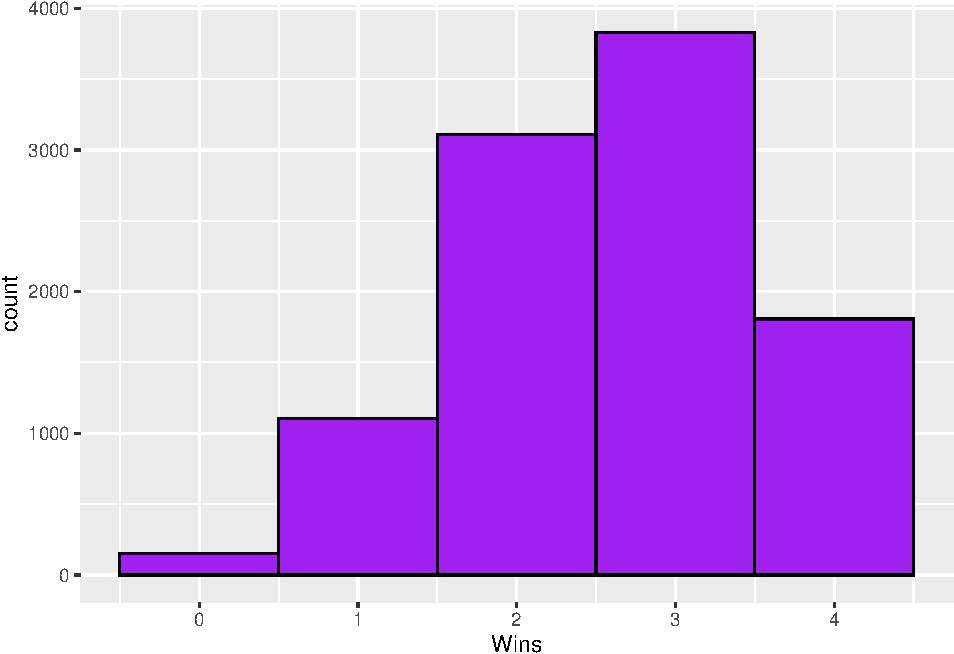
\includegraphics{textbook_files/figure-latex/unnamed-chunk-52-1.pdf}

What do you conclude from the four QQ plots?

\newpage

\hypertarget{common-random-variables}{%
\section{Common Random Variables}\label{common-random-variables}}

There are several families of random variables that show up frequently in applications. Some of these random variables include: Binomial, Geometric, Poisson, Normal

\hypertarget{binomial-rvs}{%
\subsection{Binomial RVs}\label{binomial-rvs}}

\begin{definition}
A \textbf{\emph{binomial(n,p) random variable}} is a discrete random variable that counts the numbers of ``successes'' over a fixed number of trials, \(n\), with each trial having an equal probability of success, \(p\).

\(P(X=k) = \binom{n}{k} p^k(1-p)^{n-k} = \frac{n!}{k!\ \cdot\ (n-k)!} p^k(1-p)^{n-k}\), where \(0 \leq k \leq n, 0 \leq p \leq 1\)

If \(X \sim Binomial(n,p)\), then \(E[X]=np\) and \(Var(X)=np(1-p)\)
\end{definition}

\begin{example}
The Cubs and Rockies are playing a 4-game series. The Rockies have a 0.65 probability of winning each game, and the Cubs have a 0.35 probability. Assume each game is independent. Solve for the following quantities.
\end{example}

\begin{enumerate}
\def\labelenumi{(\alph{enumi})}
\item
  The Cubs win exactly 1 game.\\
  \strut \\
  \strut \\
  \strut \\
  \vfill
\item
  The Rockies win exactly 2 games.\\
  \strut \\
  \strut \\
  \strut \\
  \vfill
\item
  The series ends in a sweep.\\
  \strut \\
  \strut \\
  \strut \\
  \vfill
\item
  The expected number of wins for the Rockies.\\
  \strut \\
  \strut \\
  \strut \\
  \vfill
\item
  The variance and standard deviations of wins for the Rockies.\\
  \strut \\
  \strut \\
  \strut \\
  \vfill
\end{enumerate}

\newpage

\begin{example}
Complete 10,000 simulations of the four game series between the Rockies and Cubs. For the number of Rockies wins, calculate the sample mean and sample variance and compare these to the population values. Also, plot a histogram of the sample data.
\end{example}

\begin{Shaded}
\begin{Highlighting}[]
\FunctionTok{set.seed}\NormalTok{(}\DecValTok{2022}\NormalTok{)}
\NormalTok{rockies\_wins }\OtherTok{\textless{}{-}} \FunctionTok{rbinom}\NormalTok{(}\AttributeTok{n=}\DecValTok{10000}\NormalTok{,}\AttributeTok{size=}\DecValTok{4}\NormalTok{,}\AttributeTok{prob=}\FloatTok{0.65}\NormalTok{)}
\FunctionTok{mean}\NormalTok{(rockies\_wins)}
\end{Highlighting}
\end{Shaded}

\begin{verbatim}
## [1] 2.6036
\end{verbatim}

\begin{Shaded}
\begin{Highlighting}[]
\FunctionTok{var}\NormalTok{(rockies\_wins)}
\end{Highlighting}
\end{Shaded}

\begin{verbatim}
## [1] 0.9121583
\end{verbatim}

\begin{Shaded}
\begin{Highlighting}[]
\NormalTok{rockies\_wins\_df }\OtherTok{\textless{}{-}} \FunctionTok{data.frame}\NormalTok{(}\AttributeTok{Wins=}\NormalTok{rockies\_wins)}
\NormalTok{rockies\_wins\_df }\SpecialCharTok{\%\textgreater{}\%} \FunctionTok{ggplot}\NormalTok{(}\FunctionTok{aes}\NormalTok{(Wins)) }\SpecialCharTok{+} \FunctionTok{geom\_histogram}\NormalTok{(}\AttributeTok{binwidth =} \DecValTok{1}\NormalTok{,}\AttributeTok{color =} \StringTok{"black"}\NormalTok{, }\AttributeTok{fill =} \StringTok{"purple"}\NormalTok{)}
\end{Highlighting}
\end{Shaded}

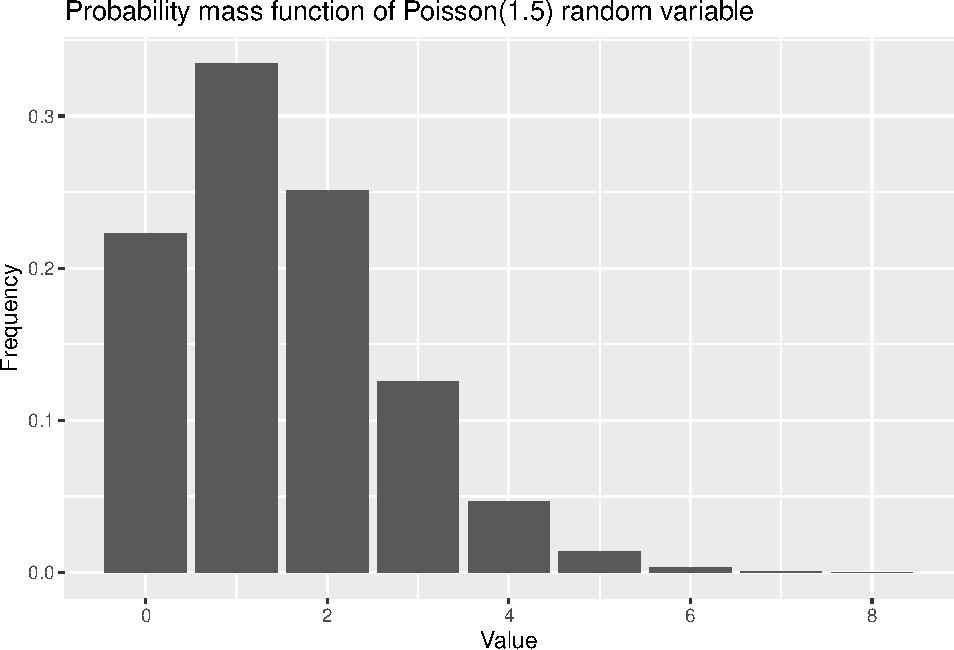
\includegraphics{textbook_files/figure-latex/unnamed-chunk-53-1.pdf}

\vfill

\newpage

\newpage

\hypertarget{geometric-rvs}{%
\subsection{Geometric RVs}\label{geometric-rvs}}

\begin{definition}
A \textbf{\emph{Geometric(p) random variable}} is a discrete random variable that counts the numbers of trials until a ``success'' occurs, where the probability of success, \(p\), is constant across all trials.

\(P(X=k) = p(1-p)^{k-1}\), where \(k \geq 1, 0 \leq p \leq 1\)

If \(X \sim Geometric(p)\), then \(E[X]=\frac{1}{p}\) and \(Var(X)=\frac{p}{1-p}\)
\end{definition}

\begin{example}
Suppose the number of shots needed by a hockey team in order to score their first goal, X, is modeled by a Geometric(\(\frac{1}{10}\)) random variable. Use this information to answer the following questions.
\end{example}

\begin{enumerate}
\def\labelenumi{(\alph{enumi})}
\item
  What is the probability that it takes exactly 3 shots to score the first goal?\\
  \strut \\
  \strut \\
  \strut \\
  \vfill
\item
  What is the probability that it takes less than 3 shots to score the first goal?\\
  \strut \\
  \strut \\
  \strut \\
  \vfill
\item
  What is the probability that it takes more than 3 shots to score the first goal?\\
  \strut \\
  \strut \\
  \strut \\
  \vfill
\item
  What is the expected number of shots to score the first goal?\\
  \strut \\
  \strut \\
  \strut \\
  \vfill
\end{enumerate}

\newpage

\textbf{Caution:} Some references parameterize the Geometric distribution based on the number of failures before the first success, rather than the trial on which the first success occurs. This changes the PMF, mean, and variance, so be careful.

Let's simulate the number of shot attempts required to score the first goal (Geometric(\(p=1/10\))) from the previous example.

\begin{Shaded}
\begin{Highlighting}[]
\FunctionTok{set.seed}\NormalTok{(}\DecValTok{2020}\NormalTok{)}
\NormalTok{geometric }\OtherTok{\textless{}{-}} \FunctionTok{rgeom}\NormalTok{(}\DecValTok{10000}\NormalTok{, }\DecValTok{1}\SpecialCharTok{/}\DecValTok{10}\NormalTok{)}
\FunctionTok{head}\NormalTok{(geometric, }\DecValTok{20}\NormalTok{)}
\end{Highlighting}
\end{Shaded}

\begin{verbatim}
##  [1]  2  2  7 55  6 11  2 11  2  5  0 50 17  2  7  0  7 19 17  1
\end{verbatim}

Some of the values were 0, which could not happen if R was considering the number of the trial on which the first success occurred. You can add 1 to the values given by \texttt{R} to arrive at the first success distribution.

\begin{Shaded}
\begin{Highlighting}[]
\NormalTok{first\_success }\OtherTok{\textless{}{-}}\NormalTok{ geometric }\SpecialCharTok{+} \DecValTok{1}
\FunctionTok{head}\NormalTok{(first\_success, }\DecValTok{20}\NormalTok{)}
\end{Highlighting}
\end{Shaded}

\begin{verbatim}
##  [1]  3  3  8 56  7 12  3 12  3  6  1 51 18  3  8  1  8 20 18  2
\end{verbatim}

\begin{Shaded}
\begin{Highlighting}[]
\NormalTok{(mean\_success }\OtherTok{\textless{}{-}} \FunctionTok{mean}\NormalTok{(first\_success))}
\end{Highlighting}
\end{Shaded}

\begin{verbatim}
## [1] 10.0669
\end{verbatim}

The mean of this sample of variables is 10.0669, which is close to the expected mean of \(\frac{1}{p} = 10\).

\newpage

Let's plot the sample distribution of shots required to score a goal from the simulation as well.

\begin{Shaded}
\begin{Highlighting}[]
\NormalTok{first\_success\_df }\OtherTok{=} \FunctionTok{data.frame}\NormalTok{(}\AttributeTok{Shots =}\NormalTok{ first\_success)}
\NormalTok{first\_success\_df }\SpecialCharTok{\%\textgreater{}\%} \FunctionTok{ggplot}\NormalTok{(}\FunctionTok{aes}\NormalTok{(}\AttributeTok{x=}\NormalTok{Shots)) }\SpecialCharTok{+} \FunctionTok{geom\_histogram}\NormalTok{(}\AttributeTok{binwidth =} \DecValTok{1}\NormalTok{)}
\end{Highlighting}
\end{Shaded}

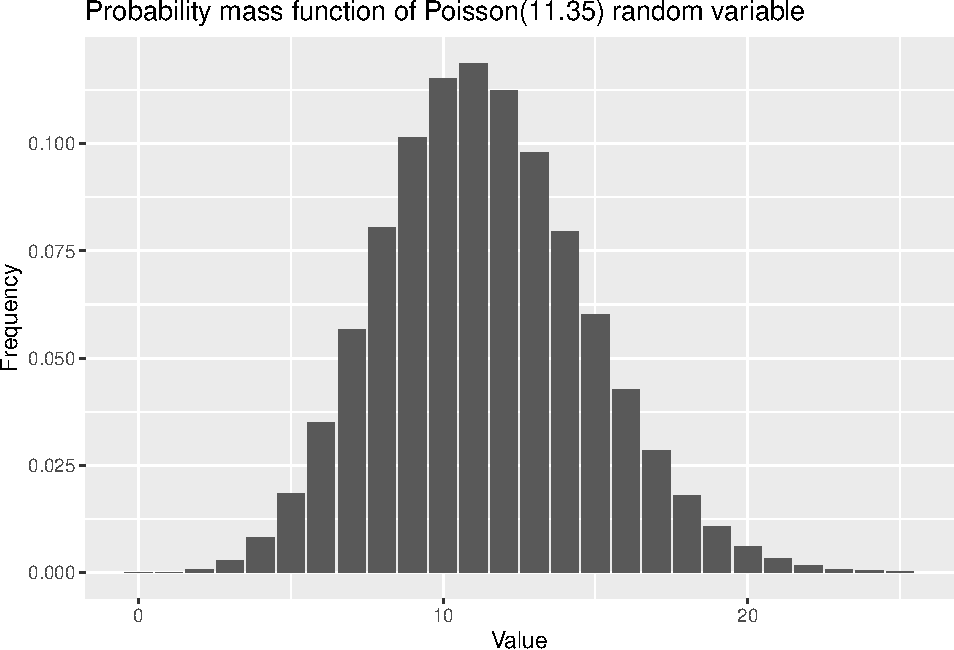
\includegraphics{textbook_files/figure-latex/unnamed-chunk-56-1.pdf}

\newpage

\hypertarget{poisson-rvs}{%
\subsection{Poisson RVs}\label{poisson-rvs}}

\begin{definition}
A \textbf{\emph{Poisson(\(\lambda\)) random variable}} is a discrete random variable that counts the numbers of ``successes'' for a given rate parameter, \(\lambda\), for a given interval.

\(P(X=k) = \frac{e^{-\lambda}\lambda^k}{k!}\), where \(k \geq 0,\)

If \(X \sim Poisson(\lambda)\), then \(E[X]=\lambda\) and \(Var(X)=\lambda\)
\end{definition}

\begin{example}
During the 2021 Major League Soccer season, the Colorado Rapids scored 51 goals in 34 games on their way to a first-place finish in the Western Conference regular season standings.

The team scored \(\frac{51}{34} = 1.5\) goals per game. Let's model the distribution of Rapids goals using a Poisson(1.5) random variable that we'll call Y.
\end{example}

\begin{enumerate}
\def\labelenumi{(\alph{enumi})}
\tightlist
\item
  Which is more likely: Y taking on the value 0 or Y taking on the value 2?\\
  \strut \\
  \strut \\
  \strut \\
\end{enumerate}

We can calculate these probabilities in R using the \texttt{dpois} command.

\begin{Shaded}
\begin{Highlighting}[]
\FunctionTok{dpois}\NormalTok{(}\AttributeTok{x=}\DecValTok{0}\NormalTok{, }\AttributeTok{lambda=}\FloatTok{1.5}\NormalTok{)}
\end{Highlighting}
\end{Shaded}

\begin{verbatim}
## [1] 0.2231302
\end{verbatim}

\begin{Shaded}
\begin{Highlighting}[]
\FunctionTok{dpois}\NormalTok{(}\AttributeTok{x=}\DecValTok{2}\NormalTok{, }\AttributeTok{lambda=}\FloatTok{1.5}\NormalTok{)}
\end{Highlighting}
\end{Shaded}

\begin{verbatim}
## [1] 0.2510214
\end{verbatim}

\newpage

We can also plot the PMF of Y to check visually.

\begin{Shaded}
\begin{Highlighting}[]
\NormalTok{x }\OtherTok{\textless{}{-}} \DecValTok{0}\SpecialCharTok{:}\DecValTok{8}
\NormalTok{y }\OtherTok{\textless{}{-}} \FunctionTok{dpois}\NormalTok{(x, }\AttributeTok{lambda =} \FloatTok{1.5}\NormalTok{)}
\NormalTok{poisson.pmf }\OtherTok{\textless{}{-}} \FunctionTok{data.frame}\NormalTok{(x,y)}
\FunctionTok{ggplot}\NormalTok{(}\FunctionTok{transform}\NormalTok{(poisson.pmf), }\FunctionTok{aes}\NormalTok{(x, y)) }\SpecialCharTok{+} 
  \FunctionTok{geom\_bar}\NormalTok{(}\AttributeTok{stat=}\StringTok{"identity"}\NormalTok{) }\SpecialCharTok{+} 
  \FunctionTok{ggtitle}\NormalTok{(}\StringTok{"Probability mass function of Poisson(1.5) random variable"}\NormalTok{) }\SpecialCharTok{+}
  \FunctionTok{xlab}\NormalTok{(}\StringTok{"Value"}\NormalTok{) }\SpecialCharTok{+}
  \FunctionTok{ylab}\NormalTok{(}\StringTok{"Probability"}\NormalTok{)}
\end{Highlighting}
\end{Shaded}

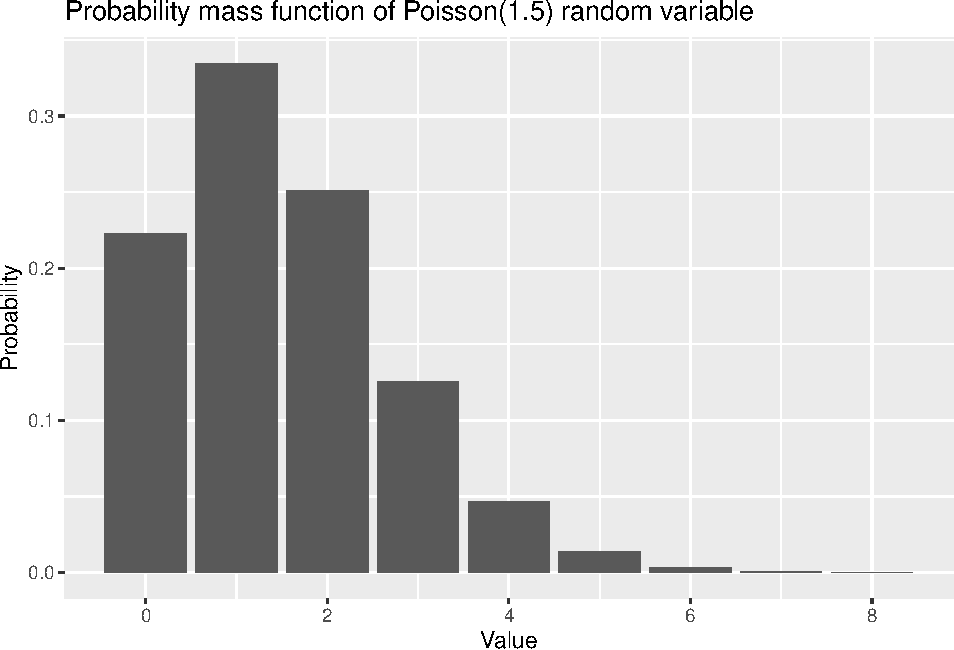
\includegraphics{textbook_files/figure-latex/unnamed-chunk-58-1.pdf}

\newpage

Let's check whether using a Poisson distribution was appropriate by comparing it to the actual 2021 Colorado Rapids match results.

\begin{Shaded}
\begin{Highlighting}[]
\CommentTok{\# Data: https://www.espn.com/soccer/team/results/\_/id/184/season/2021}

\FunctionTok{library}\NormalTok{(}\StringTok{"kableExtra"}\NormalTok{)}
\NormalTok{rapids21 }\OtherTok{\textless{}{-}} 
  \FunctionTok{c}\NormalTok{(}\DecValTok{0}\NormalTok{,}\DecValTok{1}\NormalTok{,}\DecValTok{1}\NormalTok{,}\DecValTok{3}\NormalTok{,}\DecValTok{3}\NormalTok{,}\DecValTok{1}\NormalTok{,}\DecValTok{3}\NormalTok{,}\DecValTok{2}\NormalTok{,}\DecValTok{1}\NormalTok{,}\DecValTok{1}\NormalTok{,}\DecValTok{2}\NormalTok{,}\DecValTok{1}\NormalTok{,}\DecValTok{2}\NormalTok{,}\DecValTok{0}\NormalTok{,}\DecValTok{1}\NormalTok{,}\DecValTok{0}\NormalTok{,}\DecValTok{3}\NormalTok{,}\DecValTok{2}\NormalTok{,}\DecValTok{2}\NormalTok{,}\DecValTok{1}\NormalTok{,}\DecValTok{1}\NormalTok{,}\DecValTok{1}\NormalTok{,}\DecValTok{2}\NormalTok{,}\DecValTok{1}\NormalTok{,}\DecValTok{0}\NormalTok{,}\DecValTok{3}\NormalTok{,}\DecValTok{0}\NormalTok{,}\DecValTok{3}\NormalTok{,}\DecValTok{1}\NormalTok{,}\DecValTok{1}\NormalTok{,}\DecValTok{2}\NormalTok{,}\DecValTok{0}\NormalTok{,}\DecValTok{1}\NormalTok{,}\DecValTok{5}\NormalTok{)}

\NormalTok{goals }\OtherTok{\textless{}{-}} \FunctionTok{c}\NormalTok{(}\DecValTok{0}\SpecialCharTok{:}\DecValTok{4}\NormalTok{, }\StringTok{"5+"}\NormalTok{)}
\NormalTok{actual\_frequency }\OtherTok{\textless{}{-}} \FunctionTok{c}\NormalTok{(}\DecValTok{6}\NormalTok{, }\DecValTok{14}\NormalTok{, }\DecValTok{7}\NormalTok{, }\DecValTok{6}\NormalTok{, }\DecValTok{0}\NormalTok{, }\DecValTok{1}\NormalTok{)}
\NormalTok{actual\_proportion }\OtherTok{\textless{}{-}}\NormalTok{ actual\_frequency }\SpecialCharTok{/} \FunctionTok{sum}\NormalTok{(actual\_frequency)}
\NormalTok{expected\_proportion }\OtherTok{\textless{}{-}} \FunctionTok{c}\NormalTok{(}\FunctionTok{dpois}\NormalTok{(}\DecValTok{0}\SpecialCharTok{:}\DecValTok{4}\NormalTok{, }\AttributeTok{lambda=}\FloatTok{1.5}\NormalTok{), }
                         \FunctionTok{ppois}\NormalTok{(}\DecValTok{4}\NormalTok{, }\AttributeTok{lambda=}\FloatTok{1.5}\NormalTok{, }\AttributeTok{lower.tail=}\ConstantTok{FALSE}\NormalTok{))}
\NormalTok{expected\_frequency }\OtherTok{\textless{}{-}} \FunctionTok{round}\NormalTok{(expected\_proportion }\SpecialCharTok{*} \DecValTok{34}\NormalTok{, }\DecValTok{1}\NormalTok{)}

\NormalTok{rapids.data }\OtherTok{\textless{}{-}} \FunctionTok{data.frame}\NormalTok{(goals, actual\_frequency, actual\_proportion, }
\NormalTok{                          expected\_frequency, expected\_proportion)}
\FunctionTok{names}\NormalTok{(rapids.data) }\OtherTok{=} \FunctionTok{c}\NormalTok{(}\StringTok{"Goals"}\NormalTok{,}\StringTok{"Actual Frequency"}\NormalTok{,}\StringTok{"Actual Proportion"}\NormalTok{,}\StringTok{"Expected Frequency"}\NormalTok{,}\StringTok{"Expected Proportion"}\NormalTok{)}

\NormalTok{rapids.data }\SpecialCharTok{\%\textgreater{}\%} \FunctionTok{kt}\NormalTok{()}
\end{Highlighting}
\end{Shaded}

\begin{table}[H]
\centering
\begin{tabular}{lrrrr}
\toprule
Goals & Actual Frequency & Actual Proportion & Expected Frequency & Expected Proportion\\
\midrule
0 & 6 & 0.176 & 7.6 & 0.223\\
1 & 14 & 0.412 & 11.4 & 0.335\\
2 & 7 & 0.206 & 8.5 & 0.251\\
3 & 6 & 0.176 & 4.3 & 0.126\\
4 & 0 & 0.000 & 1.6 & 0.047\\
5+ & 1 & 0.029 & 0.6 & 0.019\\
\bottomrule
\end{tabular}
\end{table}

\begin{enumerate}
\def\labelenumi{(\alph{enumi})}
\setcounter{enumi}{1}
\tightlist
\item
  What differences do you notice between the actual results and the expected values based on the Poisson random variable?\\
  \strut \\
  \strut \\
  \strut \\
  \vfill
\end{enumerate}

\begin{enumerate}
\def\labelenumi{(\alph{enumi})}
\setcounter{enumi}{2}
\tightlist
\item
  Even if the true population distribution of 2021 Rapids goals was truly a Poisson(1.5) random variable, why might the actual distribution of their goals differ from the probability mass function?\\
  \strut \\
  \strut \\
  \strut \\
  \vfill
\end{enumerate}

\newpage

\begin{enumerate}
\def\labelenumi{(\alph{enumi})}
\setcounter{enumi}{3}
\tightlist
\item
  Use a QQ plot to compare the probability distribution of the 2021 Rapids goals to a Poisson distribution.\\
\end{enumerate}

\begin{Shaded}
\begin{Highlighting}[]
\NormalTok{rapids21 }\SpecialCharTok{\%\textgreater{}\%} 
\NormalTok{  as.data.frame }\SpecialCharTok{\%\textgreater{}\%} 
  \FunctionTok{ggplot}\NormalTok{(}\FunctionTok{aes}\NormalTok{(}\AttributeTok{sample =}\NormalTok{ rapids21)) }\SpecialCharTok{+}
  \FunctionTok{stat\_qq}\NormalTok{(}\AttributeTok{distribution =}\NormalTok{ qpois,}
          \AttributeTok{dparams =} \FloatTok{1.5}\NormalTok{,}\AttributeTok{position=}\FunctionTok{position\_jitter}\NormalTok{(}\AttributeTok{width =} \FloatTok{0.1}\NormalTok{,}\AttributeTok{height =} \FloatTok{0.1}\NormalTok{)) }\SpecialCharTok{+}
  \FunctionTok{stat\_qq\_line}\NormalTok{(}\AttributeTok{distribution =}\NormalTok{ qpois, }\AttributeTok{dparams =} \FloatTok{1.5}\NormalTok{) }\SpecialCharTok{+}
  \FunctionTok{ggtitle}\NormalTok{(}\StringTok{"QQ{-}plot for Rapids 2021 Goals vs. Poisson Distribution"}\NormalTok{) }\SpecialCharTok{+}
  \FunctionTok{xlab}\NormalTok{(}\StringTok{"Theoretical Quantiles"}\NormalTok{) }\SpecialCharTok{+}
  \FunctionTok{ylab}\NormalTok{(}\StringTok{"Empirical Quantiles"}\NormalTok{)}
\end{Highlighting}
\end{Shaded}

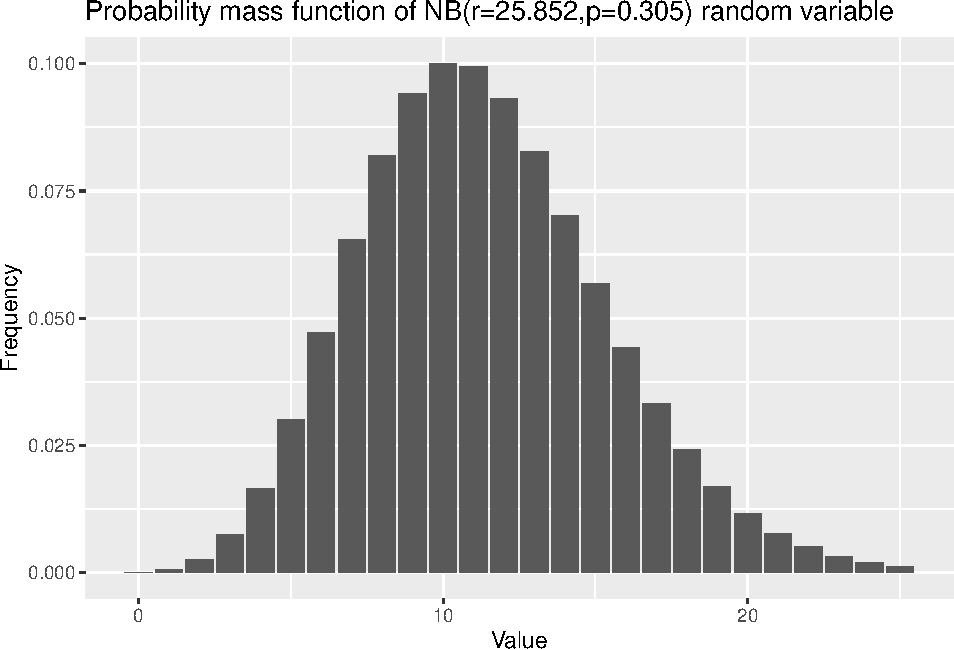
\includegraphics{textbook_files/figure-latex/unnamed-chunk-60-1.pdf}

\begin{enumerate}
\def\labelenumi{(\alph{enumi})}
\setcounter{enumi}{4}
\tightlist
\item
  What are the advantages of using the Poisson distribution to model Major League soccer goals? What are the disadvantages?\\
  \strut \\
  \strut \\
  \strut \\
\end{enumerate}

\newpage

\begin{example}
In 1997-1998 with the Los Angeles Lakers, Shaquille O'Neal attempted an average of 11.35 free throws per game with a standard deviation of 4.04. Is it appropriate to model Shaq's per game free throw attempts as a Poisson(11.35) random variable?
\end{example}

\begin{enumerate}
\def\labelenumi{(\alph{enumi})}
\tightlist
\item
  Plot the data.
\end{enumerate}

\begin{Shaded}
\begin{Highlighting}[]
\NormalTok{shaq9798 }\OtherTok{\textless{}{-}} \FunctionTok{read\_csv}\NormalTok{(}\StringTok{"data/shaq9798.csv"}\NormalTok{)}
\NormalTok{shaq9798 }\SpecialCharTok{\%\textgreater{}\%} \FunctionTok{ggplot}\NormalTok{(}\FunctionTok{aes}\NormalTok{(}\AttributeTok{x=}\NormalTok{FTA))  }\SpecialCharTok{+} 
  \FunctionTok{geom\_bar}\NormalTok{(}\AttributeTok{color =} \StringTok{"yellow"}\NormalTok{, }\AttributeTok{fill =} \StringTok{"purple"}\NormalTok{) }\SpecialCharTok{+}
  \FunctionTok{ggtitle}\NormalTok{(}\StringTok{"Per Game FT Attempt Totals by Shaq in 1997{-}1998"}\NormalTok{) }\SpecialCharTok{+}
  \FunctionTok{xlim}\NormalTok{(}\DecValTok{0}\NormalTok{,}\DecValTok{25}\NormalTok{)}
\end{Highlighting}
\end{Shaded}

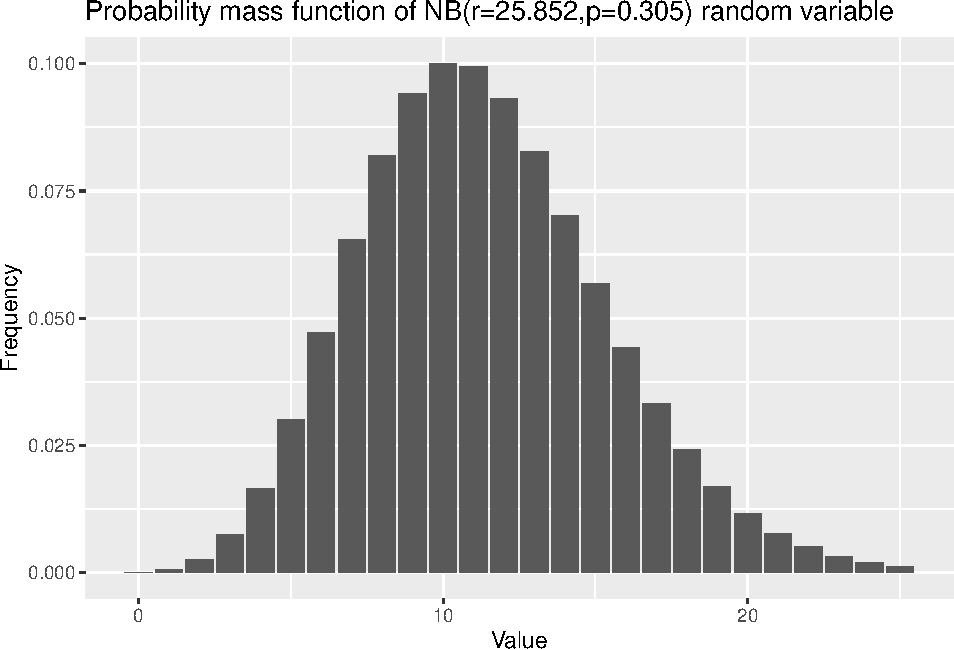
\includegraphics{textbook_files/figure-latex/unnamed-chunk-61-1.pdf}

\newpage

\begin{enumerate}
\def\labelenumi{(\alph{enumi})}
\setcounter{enumi}{1}
\tightlist
\item
  Plot the PMF of a Poisson(11.35) random variable.
\end{enumerate}

\begin{Shaded}
\begin{Highlighting}[]
\NormalTok{x }\OtherTok{\textless{}{-}} \DecValTok{0}\SpecialCharTok{:}\DecValTok{25}
\NormalTok{y }\OtherTok{\textless{}{-}} \FunctionTok{dpois}\NormalTok{(x, }\AttributeTok{lambda =} \FloatTok{11.35}\NormalTok{)}
\NormalTok{poisson.pmf }\OtherTok{\textless{}{-}} \FunctionTok{data.frame}\NormalTok{(x,y)}
\FunctionTok{ggplot}\NormalTok{(poisson.pmf, }\FunctionTok{aes}\NormalTok{(x, y)) }\SpecialCharTok{+} 
  \FunctionTok{geom\_bar}\NormalTok{(}\AttributeTok{stat=}\StringTok{"identity"}\NormalTok{) }\SpecialCharTok{+} 
  \FunctionTok{ggtitle}\NormalTok{(}\StringTok{"Probability mass function of Poisson(11.35) random variable"}\NormalTok{) }\SpecialCharTok{+}
  \FunctionTok{xlab}\NormalTok{(}\StringTok{"Value"}\NormalTok{) }\SpecialCharTok{+}
  \FunctionTok{ylab}\NormalTok{(}\StringTok{"Probability"}\NormalTok{)}
\end{Highlighting}
\end{Shaded}

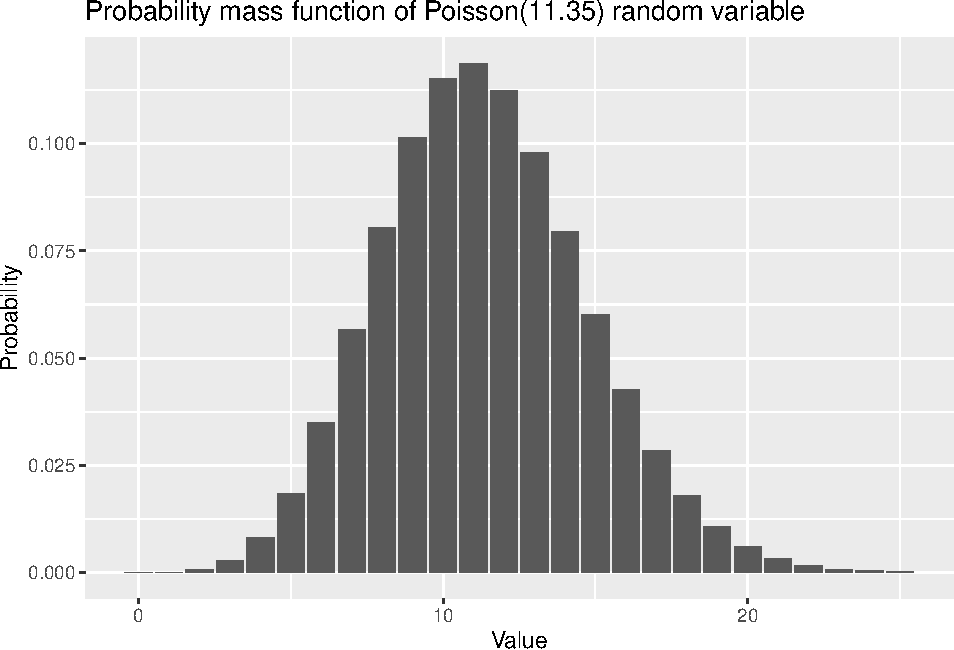
\includegraphics{textbook_files/figure-latex/unnamed-chunk-62-1.pdf}

\begin{enumerate}
\def\labelenumi{(\alph{enumi})}
\setcounter{enumi}{2}
\tightlist
\item
  What similarities and what differences do you notice?\\
  \strut \\
  \strut \\
  \strut \\
  \vfill
\end{enumerate}

\newpage

\begin{enumerate}
\def\labelenumi{(\alph{enumi})}
\setcounter{enumi}{3}
\tightlist
\item
  Calculate the variance of the two distributions and compare them.
\end{enumerate}

\begin{Shaded}
\begin{Highlighting}[]
\FunctionTok{var}\NormalTok{(shaq9798}\SpecialCharTok{$}\NormalTok{FTA)}
\end{Highlighting}
\end{Shaded}

\begin{verbatim}
## [1] 16.33305
\end{verbatim}

\begin{Shaded}
\begin{Highlighting}[]
\CommentTok{\# Var(Poisson(11.35)) = 11.35}
\end{Highlighting}
\end{Shaded}

\begin{enumerate}
\def\labelenumi{(\alph{enumi})}
\setcounter{enumi}{4}
\tightlist
\item
  Calculate the probability that Shaq had 20 or more free throws and compare it to \(P(Poisson(11.35) \geq 20)\)
\end{enumerate}

\begin{Shaded}
\begin{Highlighting}[]
\NormalTok{shaqFTA }\OtherTok{\textless{}{-}}\NormalTok{ shaq9798}\SpecialCharTok{$}\NormalTok{FTA}
\NormalTok{shaq20 }\OtherTok{\textless{}{-}} \FunctionTok{sum}\NormalTok{(shaqFTA }\SpecialCharTok{\textgreater{}=} \DecValTok{20}\NormalTok{)}\SpecialCharTok{/}\FunctionTok{length}\NormalTok{(shaqFTA); shaq20}
\end{Highlighting}
\end{Shaded}

\begin{verbatim}
## [1] 0.06666667
\end{verbatim}

\begin{Shaded}
\begin{Highlighting}[]
\NormalTok{poisson20 }\OtherTok{\textless{}{-}} \FunctionTok{ppois}\NormalTok{(}\DecValTok{20}\NormalTok{, }\AttributeTok{lambda=}\FloatTok{11.35}\NormalTok{, }\AttributeTok{lower.tail=}\ConstantTok{FALSE}\NormalTok{); poisson20}
\end{Highlighting}
\end{Shaded}

\begin{verbatim}
## [1] 0.006536079
\end{verbatim}

\newpage

\begin{enumerate}
\def\labelenumi{(\alph{enumi})}
\setcounter{enumi}{5}
\tightlist
\item
  Create a QQ-plot of Shaq's per game free throw attempts and a Poisson distribution.
\end{enumerate}

\begin{Shaded}
\begin{Highlighting}[]
\NormalTok{shaq9798 }\SpecialCharTok{\%\textgreater{}\%} 
  \FunctionTok{ggplot}\NormalTok{(}\FunctionTok{aes}\NormalTok{(}\AttributeTok{sample =}\NormalTok{ FTA)) }\SpecialCharTok{+}
  \FunctionTok{stat\_qq}\NormalTok{(}\AttributeTok{distribution =}\NormalTok{ qpois,}\AttributeTok{dparams =} \FloatTok{11.35}\NormalTok{,}\AttributeTok{position=}\FunctionTok{position\_jitter}\NormalTok{(}\AttributeTok{width=}\FloatTok{0.2}\NormalTok{,}\AttributeTok{height=}\FloatTok{0.2}\NormalTok{)) }\SpecialCharTok{+}
  \FunctionTok{stat\_qq\_line}\NormalTok{(}\AttributeTok{distribution =}\NormalTok{ qpois, }\AttributeTok{dparams =} \FloatTok{11.35}\NormalTok{) }\SpecialCharTok{+}
  \FunctionTok{ggtitle}\NormalTok{(}\StringTok{"QQ{-}plot for Shaq\textquotesingle{}s Free Throw Attempts vs. Poisson Distribution"}\NormalTok{) }\SpecialCharTok{+}
  \FunctionTok{xlab}\NormalTok{(}\StringTok{"Theoretical Quantiles"}\NormalTok{) }\SpecialCharTok{+}
  \FunctionTok{ylab}\NormalTok{(}\StringTok{"Empirical Quantiles"}\NormalTok{)}
\end{Highlighting}
\end{Shaded}

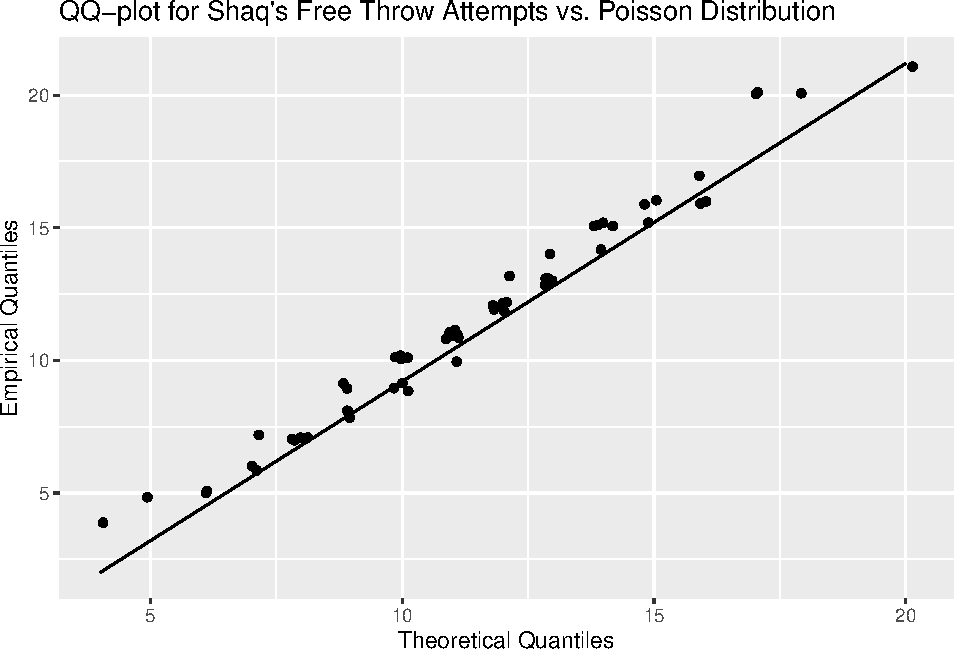
\includegraphics{textbook_files/figure-latex/unnamed-chunk-65-1.pdf}

\begin{enumerate}
\def\labelenumi{(\alph{enumi})}
\setcounter{enumi}{6}
\tightlist
\item
  Is the Poisson distribution appropriate to model Shaq's FTA per game? Explain.\\
  \strut \\
  \strut \\
  \strut \\
\end{enumerate}

\newpage

\hypertarget{negative-binomial-rvs}{%
\subsection{Negative Binomial RVs}\label{negative-binomial-rvs}}

\begin{definition}
A \textbf{\emph{Negative Binomial(\(r\),\(p\)) random variable}} is a discrete random variable that counts the numbers of ``successes'' for given parameters, \(r\) and \(p\).

\(P(X=k) = {k+r-1 \choose k}(1-p)^rp^k\), where \(k = 0, 1, 2, ...\)

If \(X \sim NB(r,p)\), then \(E[X]=\frac{rp}{1-p}\) and \(Var(X)=\frac{rp}{(1-p)^2}\)
\end{definition}

The Negative Binomial distribution is often used to model count data that is ``overdispersed''. A property of the Poisson distribution is that the mean and variance are equal. If you are analyzing count data such that the variance is much greater than the mean (i.e., overdispersed), then the Negative Binomial distribution may be an appropriate substitute.

Given sample count data, we can estimate appropriate parameters for a Negative Binomial in many ways. One such way is to use the ``method of moments'' estimator.

These estimators are given by:

\(\hat{p} = \frac{s^2-\bar{x}}{s^2}\) and \(\hat{r} = \frac{\bar{x}^2}{s^2-\bar{x}}\)

\begin{example}
Using Shaq's 1997-1998 data, model his per game free throw attempts as a Negative Binomial random variable.
\end{example}

\begin{enumerate}
\def\labelenumi{(\alph{enumi})}
\tightlist
\item
  Find an appropriate choice of parameters, \(r\) and \(p\).
\end{enumerate}

\begin{Shaded}
\begin{Highlighting}[]
\NormalTok{shaq.mean }\OtherTok{\textless{}{-}} \FunctionTok{mean}\NormalTok{(shaqFTA)}
\NormalTok{shaq.var }\OtherTok{\textless{}{-}} \FunctionTok{var}\NormalTok{(shaqFTA)}
\NormalTok{rhat }\OtherTok{\textless{}{-}}\NormalTok{ shaq.mean}\SpecialCharTok{\^{}}\DecValTok{2}\SpecialCharTok{/}\NormalTok{(shaq.var}\SpecialCharTok{{-}}\NormalTok{shaq.mean)}
\NormalTok{phat }\OtherTok{\textless{}{-}}\NormalTok{ (shaq.var}\SpecialCharTok{{-}}\NormalTok{shaq.mean)}\SpecialCharTok{/}\NormalTok{shaq.var}
\FunctionTok{c}\NormalTok{(rhat,phat)}
\end{Highlighting}
\end{Shaded}

\begin{verbatim}
## [1] 25.85213  0.30509
\end{verbatim}

\begin{enumerate}
\def\labelenumi{(\alph{enumi})}
\setcounter{enumi}{1}
\tightlist
\item
  Plot the Negative Binomial distribution. Note that R uses an alternative parameterization for \(p\). Use \(prob = 1-p\).
\end{enumerate}

\begin{Shaded}
\begin{Highlighting}[]
\NormalTok{x }\OtherTok{\textless{}{-}} \DecValTok{0}\SpecialCharTok{:}\DecValTok{25}
\NormalTok{y }\OtherTok{\textless{}{-}} \FunctionTok{dnbinom}\NormalTok{(x,}\AttributeTok{size=}\NormalTok{rhat,}\AttributeTok{prob=}\DecValTok{1}\SpecialCharTok{{-}}\NormalTok{phat)}
\NormalTok{geom.pmf }\OtherTok{\textless{}{-}} \FunctionTok{data.frame}\NormalTok{(x,y)}
\FunctionTok{ggplot}\NormalTok{(geom.pmf, }\FunctionTok{aes}\NormalTok{(x, y)) }\SpecialCharTok{+} 
  \FunctionTok{geom\_bar}\NormalTok{(}\AttributeTok{stat=}\StringTok{"identity"}\NormalTok{) }\SpecialCharTok{+} 
  \FunctionTok{labs}\NormalTok{(}\AttributeTok{x=}\StringTok{"Value"}\NormalTok{, }\AttributeTok{y=}\StringTok{"Frequency"}\NormalTok{, }\AttributeTok{title=}\StringTok{"Probability mass function of NB(r=25.852,p=0.305) random variable"}\NormalTok{)}
\end{Highlighting}
\end{Shaded}

\includegraphics{textbook_files/figure-latex/unnamed-chunk-67-1.pdf}

\begin{enumerate}
\def\labelenumi{(\alph{enumi})}
\setcounter{enumi}{2}
\tightlist
\item
  Calculate the mean and variance of the Negative Binomial and Shaq's dataset.
\end{enumerate}

\begin{Shaded}
\begin{Highlighting}[]
\NormalTok{shaq.mean }\OtherTok{\textless{}{-}} \FunctionTok{mean}\NormalTok{(shaqFTA)}
\NormalTok{shaq.var }\OtherTok{\textless{}{-}} \FunctionTok{var}\NormalTok{(shaqFTA)}
\NormalTok{NB.mean }\OtherTok{\textless{}{-}}\NormalTok{ (rhat}\SpecialCharTok{*}\NormalTok{phat)}\SpecialCharTok{/}\NormalTok{(}\DecValTok{1}\SpecialCharTok{{-}}\NormalTok{phat)}
\NormalTok{NB.var }\OtherTok{\textless{}{-}}\NormalTok{ (rhat}\SpecialCharTok{*}\NormalTok{phat)}\SpecialCharTok{/}\NormalTok{(}\DecValTok{1}\SpecialCharTok{{-}}\NormalTok{phat)}\SpecialCharTok{\^{}}\DecValTok{2}
\FunctionTok{c}\NormalTok{(shaq.mean,shaq.var)}
\end{Highlighting}
\end{Shaded}

\begin{verbatim}
## [1] 11.35000 16.33305
\end{verbatim}

\begin{Shaded}
\begin{Highlighting}[]
\FunctionTok{c}\NormalTok{(NB.mean,NB.var)}
\end{Highlighting}
\end{Shaded}

\begin{verbatim}
## [1] 11.35000 16.33305
\end{verbatim}

\begin{enumerate}
\def\labelenumi{(\alph{enumi})}
\setcounter{enumi}{3}
\tightlist
\item
  Calculate the probability that Shaq had 20 or more free throws and compare it to \(P(NB(r=25.852,p=0.305) \geq 20)\)
\end{enumerate}

\begin{Shaded}
\begin{Highlighting}[]
\NormalTok{shaq20 }\OtherTok{\textless{}{-}} \FunctionTok{sum}\NormalTok{(shaqFTA }\SpecialCharTok{\textgreater{}=} \DecValTok{20}\NormalTok{)}\SpecialCharTok{/}\FunctionTok{length}\NormalTok{(shaqFTA); shaq20}
\end{Highlighting}
\end{Shaded}

\begin{verbatim}
## [1] 0.06666667
\end{verbatim}

\begin{Shaded}
\begin{Highlighting}[]
\NormalTok{nb20 }\OtherTok{\textless{}{-}} \FunctionTok{pnbinom}\NormalTok{(}\DecValTok{20}\NormalTok{,}\AttributeTok{size=}\NormalTok{rhat,}\AttributeTok{prob=}\DecValTok{1}\SpecialCharTok{{-}}\NormalTok{phat,}\AttributeTok{lower.tail=}\ConstantTok{FALSE}\NormalTok{); nb20}
\end{Highlighting}
\end{Shaded}

\begin{verbatim}
## [1] 0.0208711
\end{verbatim}

\newpage

\begin{enumerate}
\def\labelenumi{(\alph{enumi})}
\setcounter{enumi}{4}
\tightlist
\item
  Create a QQ-plot of Shaq's per game free throw attempts and a Negative Binomial distribution.
\end{enumerate}

\begin{Shaded}
\begin{Highlighting}[]
\NormalTok{shaq9798 }\SpecialCharTok{\%\textgreater{}\%} 
  \FunctionTok{ggplot}\NormalTok{(}\FunctionTok{aes}\NormalTok{(}\AttributeTok{sample =}\NormalTok{ FTA)) }\SpecialCharTok{+}
  \FunctionTok{stat\_qq}\NormalTok{(}\AttributeTok{distribution =}\NormalTok{ qnbinom,}\AttributeTok{dparams =} \FunctionTok{list}\NormalTok{(}\AttributeTok{size=}\FloatTok{25.852}\NormalTok{,}\AttributeTok{mu=}\FloatTok{11.35}\NormalTok{),}\AttributeTok{position=}\FunctionTok{position\_jitter}\NormalTok{(}\AttributeTok{width=}\FloatTok{0.2}\NormalTok{,}\AttributeTok{height=}\FloatTok{0.2}\NormalTok{)) }\SpecialCharTok{+}
  \FunctionTok{stat\_qq\_line}\NormalTok{(}\AttributeTok{distribution =}\NormalTok{ qnbinom, }\AttributeTok{dparams =} \FunctionTok{list}\NormalTok{(}\AttributeTok{size=}\FloatTok{25.852}\NormalTok{,}\AttributeTok{mu=}\FloatTok{11.35}\NormalTok{)) }\SpecialCharTok{+}
  \FunctionTok{ggtitle}\NormalTok{(}\StringTok{"QQ{-}plot for Shaq\textquotesingle{}s Free Throw Attempts vs. Negative Binomial Distribution"}\NormalTok{) }\SpecialCharTok{+}
  \FunctionTok{xlab}\NormalTok{(}\StringTok{"Theoretical Quantiles"}\NormalTok{) }\SpecialCharTok{+}
  \FunctionTok{ylab}\NormalTok{(}\StringTok{"Empirical Quantiles"}\NormalTok{)}
\end{Highlighting}
\end{Shaded}

\includegraphics{textbook_files/figure-latex/unnamed-chunk-70-1.pdf}

\begin{enumerate}
\def\labelenumi{(\alph{enumi})}
\setcounter{enumi}{5}
\tightlist
\item
  Is the Negative Binomial distribution appropriate to model Shaq's FTA per game? How does it compare to using the Poisson distribution? Explain.\\
  \strut \\
  \strut \\
  \strut \\
\end{enumerate}

\newpage

\hypertarget{normal-rvs}{%
\subsection{Normal RVs}\label{normal-rvs}}

\begin{definition}
A \textbf{\emph{Normal(\(\mu\),\(\sigma^2\)) random variable}} is a continuous random variable that is bell-shaped with mean \(\mu\) and variance \(\sigma^2\).

To calculate probabilities under the normal curve, you need either to integrate, use a table, or a computer.

Note that a normal random variable can be standardized by using: \(z = \frac{x-\mu}{\sigma}\)
\end{definition}

\begin{theorem}
For a normal(\(\mu\),\(\sigma^2\)) random variable, we have the following approximations:\\
- About 68\% of the data falls within one standard deviation of the mean (i.e., \(\mu \pm \sigma\))\\
- About 95\% of the data falls within two standard deviations of the mean (i.e., \(\mu \pm 2\sigma\))\\
- About 99.7\% of the data falls within three standard deviations of the mean (i.e., \(\mu \pm 3\sigma\))
\end{theorem}

\begin{example}
The skills (or tools) of a baseball player are often rated on a scale of 20-80, where 50 is an average grade, 20 is the lowest grade, and 80 is the highest grade. The distribution of tool grades is approximately normally distributed (\(\mu=50, \sigma =10\)).

See \url{https://blogs.fangraphs.com/scouting-explained-the-20-80-scouting-scale/} for more details. Calculate the following probabilities.
\end{example}

\begin{enumerate}
\def\labelenumi{(\alph{enumi})}
\item
  Former Rockie Nolan Arenado has been graded to have game power of 70. Game power estimates a player's ability to hit home runs. Approximately what percentage of baseball players have equal or greater game power than Arenado?\\
  \strut \\
  \strut \\
  \strut \\
  \vfill
\item
  Mike Trout has been graded to have raw power of 55. Raw power estimates a player's ability to hit baseballs hard (i.e., hard hit rate). Approximately what percentage of baseball players have equal or less raw power than Trout?\\
  \strut \\
  \strut \\
  \strut \\
  \vfill
\end{enumerate}

\newpage

\begin{enumerate}
\def\labelenumi{(\alph{enumi})}
\setcounter{enumi}{2}
\item
  Suppose a Rockies prospect is said to be in the top 10\% of all baseball players in terms of their speed. What approximate speed grade would correspond to the player?\\
  \strut \\
  \strut \\
  \strut \\
  \vfill
  x
\item
  Suppose a Rockies prospect is said to be in the bottom 20\% of all baseball players in terms of their hit ability. What approximate hit grade would correspond to the player?\\
  \strut \\
  \strut \\
  \strut \\
  \vfill
\item
  Between what two grades do approximately 95\% of all players lie for a given tool?\\
  \strut \\
  \strut \\
  \strut \\
  \vfill
\end{enumerate}

Let's check our answers:

\begin{Shaded}
\begin{Highlighting}[]
\NormalTok{a }\OtherTok{\textless{}{-}} \DecValTok{1}\SpecialCharTok{{-}}\FunctionTok{pnorm}\NormalTok{(}\AttributeTok{q=}\DecValTok{70}\NormalTok{,}\AttributeTok{mean=}\DecValTok{50}\NormalTok{,}\AttributeTok{sd=}\DecValTok{10}\NormalTok{); a}
\end{Highlighting}
\end{Shaded}

\begin{verbatim}
## [1] 0.02275013
\end{verbatim}

\begin{Shaded}
\begin{Highlighting}[]
\NormalTok{b }\OtherTok{\textless{}{-}} \FunctionTok{pnorm}\NormalTok{(}\AttributeTok{q=}\DecValTok{55}\NormalTok{,}\AttributeTok{mean=}\DecValTok{50}\NormalTok{,}\AttributeTok{sd=}\DecValTok{10}\NormalTok{); b}
\end{Highlighting}
\end{Shaded}

\begin{verbatim}
## [1] 0.6914625
\end{verbatim}

\begin{Shaded}
\begin{Highlighting}[]
\NormalTok{c }\OtherTok{\textless{}{-}} \FunctionTok{qnorm}\NormalTok{(}\FloatTok{0.1}\NormalTok{,}\AttributeTok{mean=}\DecValTok{50}\NormalTok{,}\AttributeTok{sd=}\DecValTok{10}\NormalTok{,}\AttributeTok{lower.tail =}\NormalTok{ F); c}
\end{Highlighting}
\end{Shaded}

\begin{verbatim}
## [1] 62.81552
\end{verbatim}

\begin{Shaded}
\begin{Highlighting}[]
\NormalTok{d }\OtherTok{\textless{}{-}} \FunctionTok{qnorm}\NormalTok{(}\FloatTok{0.2}\NormalTok{,}\AttributeTok{mean=}\DecValTok{50}\NormalTok{,}\AttributeTok{sd=}\DecValTok{10}\NormalTok{,}\AttributeTok{lower.tail =}\NormalTok{ T); d}
\end{Highlighting}
\end{Shaded}

\begin{verbatim}
## [1] 41.58379
\end{verbatim}

\begin{Shaded}
\begin{Highlighting}[]
\NormalTok{e }\OtherTok{\textless{}{-}} \FunctionTok{pnorm}\NormalTok{(}\AttributeTok{q=}\DecValTok{70}\NormalTok{,}\AttributeTok{mean=}\DecValTok{50}\NormalTok{,}\AttributeTok{sd=}\DecValTok{10}\NormalTok{) }\SpecialCharTok{{-}} \FunctionTok{pnorm}\NormalTok{(}\AttributeTok{q=}\DecValTok{30}\NormalTok{,}\AttributeTok{mean=}\DecValTok{50}\NormalTok{,}\AttributeTok{sd=}\DecValTok{10}\NormalTok{); e}
\end{Highlighting}
\end{Shaded}

\begin{verbatim}
## [1] 0.9544997
\end{verbatim}

\newpage

\newpage

\hypertarget{win-probability-models}{%
\section{Win Probability Models}\label{win-probability-models}}

The probability an NFL team will win can be modeled as a normal random variable using the Vegas line. This method is outlined by Wayne Winston in \emph{Mathletics} building on previous research by Hal Stern.

\hypertarget{estimating-pregame-win-probability}{%
\subsection{Estimating Pregame Win Probability}\label{estimating-pregame-win-probability}}

Winston estimates that the final margin of victory is approximately a normal random variable with a mean of the Vegas line and a standard deviation between 13-14. Winston and Stern estimated the standard deviation to be \textbf{13.86} based on data from the 1981, 1983, and 1984 NFL seasons.

This estimated standard deviation has since been updated to be \textbf{13.45} based on data from 1978 -- 2012 NFL seasons.

Reference: \url{https://www.pro-football-reference.com/about/win_prob.htm}

\begin{example}
Sketch the distribution of the final margin of victory for an NFL team that is favored by 7 points. Shade the area for a win in regulation (for the favorite) and a tie in regulation.
\end{example}

\begin{Shaded}
\begin{Highlighting}[]
\FunctionTok{library}\NormalTok{(ggplot2)}
\CommentTok{\# library(gridExtra)}


\NormalTok{final\_margin\_full }\OtherTok{\textless{}{-}} \FunctionTok{ggplot}\NormalTok{(}\FunctionTok{data.frame}\NormalTok{(}\AttributeTok{x =} \FunctionTok{c}\NormalTok{(}\SpecialCharTok{{-}}\DecValTok{21}\NormalTok{, }\DecValTok{42}\NormalTok{)), }\FunctionTok{aes}\NormalTok{(}\AttributeTok{x =}\NormalTok{ x)) }\SpecialCharTok{+}
        \FunctionTok{stat\_function}\NormalTok{(}\AttributeTok{fun =}\NormalTok{ dnorm, }\AttributeTok{args =} \FunctionTok{list}\NormalTok{(}\AttributeTok{mean =} \DecValTok{7}\NormalTok{, }\AttributeTok{sd =} \FloatTok{13.45}\NormalTok{)) }\SpecialCharTok{+} 
  \FunctionTok{xlab}\NormalTok{(}\StringTok{"Final Margin (for favorite)"}\NormalTok{) }\SpecialCharTok{+} \FunctionTok{ggtitle}\NormalTok{(}\StringTok{"Score Distribution"}\NormalTok{)}
\NormalTok{final\_margin\_full}
\end{Highlighting}
\end{Shaded}

\includegraphics{textbook_files/figure-latex/unnamed-chunk-72-1.pdf}

\newpage

\begin{example}
In Super Bowl 50, the Denver Broncos were 5.5 point underdogs (+5.5) against the Carolina Panthers. Estimate the pregame win probability for the Denver Broncos.\\

\end{example}

\includegraphics{textbook_files/figure-latex/unnamed-chunk-73-1.pdf}

\vfill

\begin{Shaded}
\begin{Highlighting}[]
\NormalTok{fav\_line }\OtherTok{\textless{}{-}} \FloatTok{5.5}
\NormalTok{full\_sd }\OtherTok{\textless{}{-}} \FloatTok{13.45}

\NormalTok{win\_prob }\OtherTok{\textless{}{-}} \FunctionTok{pnorm}\NormalTok{(}\AttributeTok{q =} \FloatTok{0.5}\NormalTok{, }\AttributeTok{mean =}\NormalTok{ fav\_line, }\AttributeTok{sd =}\NormalTok{ full\_sd, }\AttributeTok{lower.tail =} \ConstantTok{FALSE}\NormalTok{)}

\NormalTok{tie\_prob }\OtherTok{\textless{}{-}} \FunctionTok{pnorm}\NormalTok{(}\AttributeTok{q =} \FloatTok{0.5}\NormalTok{, }\AttributeTok{mean =}\NormalTok{ fav\_line, }\AttributeTok{sd =}\NormalTok{ full\_sd, }\AttributeTok{lower.tail =} \ConstantTok{TRUE}\NormalTok{) }\SpecialCharTok{{-}}
            \FunctionTok{pnorm}\NormalTok{(}\AttributeTok{q =} \SpecialCharTok{{-}}\FloatTok{0.5}\NormalTok{, }\AttributeTok{mean =}\NormalTok{ fav\_line, }\AttributeTok{sd =}\NormalTok{ full\_sd, }\AttributeTok{lower.tail =} \ConstantTok{TRUE}\NormalTok{)}

\CommentTok{\# win probability for favorite (panthers)}
\NormalTok{win\_prob }\OtherTok{\textless{}{-}}\NormalTok{ win\_prob }\SpecialCharTok{+} \DecValTok{1}\SpecialCharTok{/}\DecValTok{2} \SpecialCharTok{*}\NormalTok{ tie\_prob}

\CommentTok{\# win probability for underdog (broncos)}
\NormalTok{(broncos\_win\_prob }\OtherTok{\textless{}{-}} \DecValTok{1} \SpecialCharTok{{-}}\NormalTok{ win\_prob)}
\end{Highlighting}
\end{Shaded}

\begin{verbatim}
## [1] 0.3414021
\end{verbatim}

\newpage

\hypertarget{estimating-in-game-win-probability}{%
\subsection{Estimating In-Game Win Probability}\label{estimating-in-game-win-probability}}

Winston proposed an updated method to calculate in-game win probabilities based on the time remaining in the game, current score margin, and Vegas line.

In this proposed method, the pregame mean (Vegas line) and pregame variance (13.45) are scaled down linearly as a function of time remaining in the game.

For instance, since there are four 15-minute quarters (total regulation game time is 60 minutes), then the in-game mean and standard deviation are calculated as follows.

\(\mu_{updated} = Line \cdot \frac{\text{time remaining}}{60}\)

\(\sigma_{updated} = \frac{13.45}{\sqrt{60/\text{time remaining}}}\)

\textbf{Note:} This model assumes perfectly neutral possession, down, distance, and field-position conditions.

Reference: \url{https://www.pro-football-reference.com/about/win_prob.htm}

\begin{example}
In Super Bowl 50, the Denver Broncos led the Carolina Panthers 10-0 after the first quarter. The Broncos were 5.5 point underdogs at the start of the game. Use Winston's method to estimate the probability of a Broncos win after one quarter.\\

\end{example}

\begin{Shaded}
\begin{Highlighting}[]
\NormalTok{fav\_margin }\OtherTok{\textless{}{-}} \SpecialCharTok{{-}}\DecValTok{10}
\NormalTok{fav\_line }\OtherTok{\textless{}{-}} \FloatTok{5.5}
\NormalTok{full\_sd }\OtherTok{\textless{}{-}} \FloatTok{13.45}
\NormalTok{full\_min }\OtherTok{\textless{}{-}} \DecValTok{60}
\NormalTok{new\_min }\OtherTok{\textless{}{-}} \DecValTok{45}

\NormalTok{new\_mean }\OtherTok{\textless{}{-}}\NormalTok{ fav\_line }\SpecialCharTok{*}\NormalTok{ new\_min}\SpecialCharTok{/}\NormalTok{full\_min}
\NormalTok{new\_sd }\OtherTok{\textless{}{-}}\NormalTok{ full\_sd }\SpecialCharTok{/} \FunctionTok{sqrt}\NormalTok{(full\_min}\SpecialCharTok{/}\NormalTok{new\_min)}

\NormalTok{win\_prob }\OtherTok{\textless{}{-}} \FunctionTok{pnorm}\NormalTok{(}\AttributeTok{q =} \FloatTok{0.5} \SpecialCharTok{{-}}\NormalTok{ fav\_margin, }\AttributeTok{mean =}\NormalTok{ new\_mean, }
                  \AttributeTok{sd =}\NormalTok{ new\_sd, }\AttributeTok{lower.tail =} \ConstantTok{FALSE}\NormalTok{)}

\NormalTok{tie\_prob }\OtherTok{\textless{}{-}} \FunctionTok{pnorm}\NormalTok{(}\AttributeTok{q =} \FloatTok{0.5} \SpecialCharTok{{-}}\NormalTok{ fav\_margin, }\AttributeTok{mean =}\NormalTok{ new\_mean, }
                  \AttributeTok{sd =}\NormalTok{ new\_sd, }\AttributeTok{lower.tail =} \ConstantTok{TRUE}\NormalTok{) }\SpecialCharTok{{-}}
            \FunctionTok{pnorm}\NormalTok{(}\AttributeTok{q =} \SpecialCharTok{{-}}\FloatTok{0.5} \SpecialCharTok{{-}}\NormalTok{ fav\_margin, }\AttributeTok{mean =}\NormalTok{ new\_mean, }
                  \AttributeTok{sd =}\NormalTok{ new\_sd, }\AttributeTok{lower.tail =} \ConstantTok{TRUE}\NormalTok{)}

\CommentTok{\# win probability for favorite (panthers)}
\NormalTok{win\_prob }\OtherTok{\textless{}{-}}\NormalTok{ win\_prob }\SpecialCharTok{+} \DecValTok{1}\SpecialCharTok{/}\DecValTok{2} \SpecialCharTok{*}\NormalTok{ tie\_prob}

\CommentTok{\# win probability for underdog (broncos)}
\NormalTok{(broncos\_win\_prob }\OtherTok{\textless{}{-}} \DecValTok{1} \SpecialCharTok{{-}}\NormalTok{ win\_prob)}
\end{Highlighting}
\end{Shaded}

\begin{verbatim}
## [1] 0.6928385
\end{verbatim}

\newpage

The win probability models outlined above use only the Vegas line, the current score, and the time remaining in the game. More accurate estimation models will also consider possession, down, distance, and field-position conditions. Pro Football Reference offers an in-game win probability model with these additional factors.

Reference: \url{https://www.pro-football-reference.com/boxscores/win_prob.cgi}

\begin{example}
The Broncos led the Panthers 10-0 at the end of the first quarter. The Panthers had 2nd and 11 at their own 46 at the beginning of the second quarter. Calculate the Broncos win probability.

Reference: \url{https://www.pro-football-reference.com/boxscores/201602070den.htm}
\end{example}

\begin{figure}
\centering
\includegraphics[width=0.8\textwidth,height=\textheight]{images/wp1}
\caption{Pro Football Reference Win Probability Calculator Inputs}
\end{figure}

\begin{figure}
\centering
\includegraphics[width=0.5\textwidth,height=\textheight]{images/wp2}
\caption{Pro Football Reference Win Probability Calculator Output}
\end{figure}

\textbf{Class Reading:} Chapters 6--7 in the \emph{Hidden Game of Football} by Carroll, Palmer, Thorn

\hypertarget{odds-and-bets}{%
\chapter{Odds and Bets}\label{odds-and-bets}}

\textbf{Sports Betting in USA}

In 2018, the United States Supreme Court overturned a 1992 federal law that banned commercial sports betting in most states. For more about this ruling, see this New York Times article: \url{https://www.nytimes.com/2018/05/14/us/politics/supreme-court-sports-betting-new-jersey.html}

In Colorado, you must be at least 21 years old to gamble including betting on sports games.

\textbf{Gambling Addiction}

Gambling addiction, compulsive gambling, or gambling disorder is a serious impulse-control disorder. Here is a link to the Mayo Clinic's discussion of compulsive gambling: \url{https://www.mayoclinic.org/diseases-conditions/compulsive-gambling/symptoms-causes/syc-20355178}

Gambling is \textbf{\emph{not}} encouraged and can lead to numerous problems. If you choose to gamble on sports, don't bet beyond your means and seek help if you worry that you may be suffering from gambling addiction.

\newpage

\hypertarget{odds}{%
\section{Odds}\label{odds}}

In the previous chapter, we quantified uncertainty using probabilities (numbers between 0 and 1) and percentages (numbers between 0 and 100). We can also quantify uncertainty using \textbf{odds}.

\begin{definition}
The \textbf{\emph{odds}} (in favor) of an outcome \(A\) is the probability of \(A\) divided by the probability of \(A^C\).

\[Odds = \frac{p}{1-p}\]
\end{definition}

\textbf{Note:} We may also be given the \textbf{odds against} a particular outcome. In this case, we have \(Odds Against = \frac{1-p}{p}\).\\

\textbf{Some Common Odds:}

\begin{table}[H]
\centering
\begin{tabular}{lrrlrr}
\toprule
Odds & p & q & Odds & p & q\\
\midrule
0:1 & 0.000 & 1.000 & 1:0 & 1.000 & 0.000\\
1:1 & 0.500 & 0.500 & 1:1 & 0.500 & 0.500\\
2:1 & 0.667 & 0.333 & 1:2 & 0.333 & 0.667\\
3:1 & 0.750 & 0.250 & 1:3 & 0.250 & 0.750\\
4:1 & 0.800 & 0.200 & 1:4 & 0.200 & 0.800\\
5:1 & 0.833 & 0.167 & 1:5 & 0.167 & 0.833\\
10:1 & 0.909 & 0.091 & 1:10 & 0.091 & 0.909\\
100:1 & 0.990 & 0.010 & 1:100 & 0.010 & 0.990\\
\bottomrule
\end{tabular}
\end{table}

In the following table, the odds of an outcome along with the probability of the outcome, \emph{p}, and the probability of the outcome's complement, \emph{q=1-p} are given.

\newpage

\begin{example}
For the following examples, convert between probability and odds.
\end{example}

\begin{enumerate}
\def\labelenumi{(\alph{enumi})}
\tightlist
\item
  Suppose that the probability that the Cubs win the 2025 World Series is 0.03. What are the odds in favor?\\
\end{enumerate}

\vfill

\begin{enumerate}
\def\labelenumi{(\alph{enumi})}
\setcounter{enumi}{1}
\tightlist
\item
  Suppose that the odds against that the Rockies win the World Series in 2025 is 100:1. What is the probability in favor?\\
\end{enumerate}

\vfill

\begin{enumerate}
\def\labelenumi{(\alph{enumi})}
\setcounter{enumi}{2}
\tightlist
\item
  Suppose there is a 1\% chance that CSU wins a national championship in any sport in the next decade. What are the probability and the odds against CSU winning a national championship in the next decade?\\
\end{enumerate}

\vfill

\begin{example}
Suppose that there are three finalists in an Olympic competition. It is estimated that Athlete A has a 50\% chance of winning, Athlete B has a 40\% chance of winning, and Player C has a 10\% chance of winning. Calculate the odds against each of the athletes winning the competition.
\end{example}

\vfill

\newpage

\hypertarget{gambling-odds}{%
\section{Gambling Odds}\label{gambling-odds}}

Here's a helpful resource on calculating gambling odds:\\
\url{https://www.actionnetwork.com/education/decimal-odds}

Gambling odds are a bit different that odds in a probability context. Gambling odds tell the amount that the bookmaker will pay out for a winning bet. For example, if a bookmaker is offering ``10:1'' that the Rockies win the next World Series, the bookmaker will pay out 10x the original wager plus the original wager if the Rockies win the World Series and the bookmaker will keep the original bet if the Rockies fail to win the World Series.

\begin{definition}
The \textbf{\emph{implied probability}}, \(\tilde{p}\), of a wager is the probability that corresponds to the odds of the wager.

\[\tilde{p} = \frac{Odds}{Odds+1}, \text{where } \tilde{p} = \text{implied probability}\]
\end{definition}

\begin{definition}
\textbf{\emph{Fractional odds}} are common in horse racing and quote the net total that will be paid out to the bettor, should he or she win, relative to the stake. The numerator and denominator of fractional odds are always positive integers. For example, a \$100 wager on a ``5:1'' bet would result in a payout of \(5 \cdot \$100 + \$100 = \$600\) if the wager is correct and a payout of \$0 if the wager is incorrect.
\end{definition}

\begin{definition}
\textbf{\emph{Decimal Odds}} represent the multiplier of a winning bet and is calculated by taking the inverse of the implied probability. For instance, if you bet \$100 with decimal odds of 1.8, your payout is \$180 (\$100 wager + \$80 winnings).

\[Decimal \, Odds = [\tilde{p}]^{-1}\]
\end{definition}

\newpage

\hypertarget{types-of-bets}{%
\section{Types of Bets}\label{types-of-bets}}

\begin{definition}
A \emph{moneyline bet}, a common bet in American sports, refers to the odds of a straight-up outcome on a game without consideration of a point spread. Typically, favorites will have negative moneyline odds and underdogs will have a positive moneyline odds.

When the moneyline is positive, the figure tells what the winning payout would be on a \$100 bet.

\[\tilde{p} = \frac{100}{ML_{POS}+100}\]

When the moneyline is negative, the figure tells what wager is required for a winning payout of \$100.

\[\tilde{p} = \frac{-ML_{NEG}}{-ML_{NEG}+100}\]
\end{definition}

\begin{example}
For the following scenarios, assume a wager of \$100. Calculate the payout for a winning bet and the implied probability of that bet.
\end{example}

\begin{enumerate}
\def\labelenumi{(\alph{enumi})}
\tightlist
\item
  Fractional odds of 4/1\\
\end{enumerate}

\vfill

\begin{enumerate}
\def\labelenumi{(\alph{enumi})}
\setcounter{enumi}{1}
\tightlist
\item
  Moneyline +400\\
\end{enumerate}

\vfill

\begin{enumerate}
\def\labelenumi{(\alph{enumi})}
\setcounter{enumi}{2}
\tightlist
\item
  Moneyline -300\\
\end{enumerate}

\vfill

\begin{enumerate}
\def\labelenumi{(\alph{enumi})}
\setcounter{enumi}{3}
\tightlist
\item
  Decimal Odds of 1.5\\
\end{enumerate}

\vfill

\newpage

\begin{definition}
A \emph{moneyline bet} refers to the odds of a straight-up outcome on a game without consideration of a point spread. Typically, favorites will have negative moneyline odds and underdogs will have a positive moneyline odds.

If ML is negative:
\[\tilde{p} = \frac{-ML_{NEG}}{-ML_{NEG}+100}\]

If ML is positive:
\[\tilde{p} = \frac{100}{ML_{POS}+100}\]
\end{definition}

\begin{example}
Calculate the implied probabilities for the following examples.
\end{example}

\begin{enumerate}
\def\labelenumi{(\alph{enumi})}
\item
  Fractional odds of 4/1\\
  \strut \\
  \strut \\
  \strut \\
  \vfill
\item
  Moneyline -125\\
  \strut \\
  \strut \\
  \strut \\
  \vfill
\item
  Moneyline +125\\
  \strut \\
  \strut \\
  \strut \\
  \vfill
\item
  Decimal Odds of 1.5\\
  \strut \\
  \strut \\
  \strut \\
  \vfill
\end{enumerate}

\newpage

\begin{example}
Suppose that for an upcoming NFL game, a moneyline wager on the Broncos is -105 and a moneyline wager on the Raiders is -120.
\end{example}

\begin{enumerate}
\def\labelenumi{(\alph{enumi})}
\item
  Calculate the implied probabilities of the two possible outcomes. (Note that sometime ties are an optional wager. Other times, ties will result in a push, that is, no winner.)\\
  \strut \\
  \strut \\
  \strut \\
  \vfill
\item
  What is the sum of the implied probabilities?\\
  \strut \\
  \strut \\
  \strut \\
  \vfill
\item
  Does the result from (b) violate the axioms of probability? If so, why?\\
  \strut \\
  \strut \\
  \strut \\
  \vfill
\end{enumerate}

\textbf{Note:} The goal of bookmaking is to make money, so there will be almost certainly be a house advantage. This means that the sum of the implied probabilities will be greater than 1.

\begin{definition}
The \textbf{\emph{house advantage}} (or \textbf{\emph{hold percentage}}) is the percentage of money that sportsbooks keep for every dollar earned.

\[House \, Advantage = 100 \cdot \sum_{i=1}^n \tilde{p}_i - 100\]
\end{definition}

\begin{example}
What is the house advantage in the previous example?
\end{example}

\hfill\break
\hfill\break
\hfill\break
\vfill

\newpage

\begin{definition}
A \textbf{\emph{point spread bet}} is a bet based on the projected margin of victory that can result in a win, loss, or push.

For example, if a sports book offers Rockies -1.5 against the Cubs and you bet on the Rockies, if the Rockies win by 2 or more runs, you win and if the Rockies win by 1 run or lose, then you lose.
\end{definition}

\begin{example}
Suppose a sports book offers Broncos +14 against the Raiders at -110 (they also offer Raiders -14 at -110) and you have \$20 to wager. Calculate the payout for the following scenarios.
\end{example}

\begin{enumerate}
\def\labelenumi{(\alph{enumi})}
\item
  You bet \$20 on the Broncos and the final score is Broncos 21 Raiders 20. What is your payout?\\
  \strut \\
  \strut \\
  \strut \\
  \vfill
\item
  You bet \$20 on the Raiders and the final score is Broncos 21 Raiders 20. What is your payout?\\
  \strut \\
  \strut \\
  \strut \\
  \vfill
\item
  You bet \$10 on the Broncos and \$10 on the Raiders and the final score is Broncos 21 Raiders 20. What is your payout?\\
  \strut \\
  \strut \\
  \strut \\
  \vfill
\end{enumerate}

\begin{definition}
A \textbf{\emph{parlay bet}} is a combination of multiple bets where the winnings from a winning bet are placed on other bets. All bets must be win for the parlay bet to pay out.
\end{definition}

\newpage

\begin{example}
Suppose that CSU is a three point favorite (-3) against CU in a women's basketball game and the over/under on total number of points is 97. Assume that the price of bets is -110.
\end{example}

\begin{enumerate}
\def\labelenumi{(\alph{enumi})}
\item
  Suppose you place two \$20 bets bets, CSU -3 and Over 97, and the outcome of the game is CSU 60 CU 40. What is your payout?\\
  \strut \\
  \strut \\
  \strut \\
  \vfill
\item
  Suppose you place a \$40 parlay bet on CSU -3 and Over 97 and the outcome of the game is CSU 60 CU 40. What is your payout?\\
  \strut \\
  \strut \\
  \strut \\
  \vfill
\item
  Suppose you place two \$20 bets, CSU -3 and Over 97, and the outcome of the game is CSU 44 CU 40. What is your payout?\\
  \strut \\
  \strut \\
  \strut \\
  \vfill
\item
  Suppose you place a \$40 parlay bet on CSU -3 and Over 97 and the outcome of the game is CSU 44 CU 40. What is your payout?\\
  \strut \\
  \strut \\
  \strut \\
  \vfill
\end{enumerate}

\hypertarget{monte-carlo-simulation}{%
\chapter{Monte Carlo Simulation}\label{monte-carlo-simulation}}

\hypertarget{basics}{%
\section{Basics}\label{basics}}

Monte Carlo Simulation is a collection of computer-driven, computational algorithms that use repeated random sampling to calculate estimates. The basic steps for such a simulation are as follows:

\begin{enumerate}
\def\labelenumi{\arabic{enumi})}
\item
  Set seed for replicability
\item
  Initialize all variables/vectors
\item
  Loop through ``n'' simulations and save simulated values
\item
  Analyze the simulated values from the ``n'' simulations
\end{enumerate}

One function that will be particularly useful for simulation is \texttt{set.seed()}.

\texttt{set.seed()} allows us to replicate any simulation by giving the initial seed for the simulation. The actual number that is ``seeded'' is not particularly important though if you want to replicate the same simulations, you will want to re-use this number.

\vfill
\newpage

\begin{example}
Simulate 10 overtime coin tosses with and without using \texttt{set.seed()} and compare the results
\end{example}

\begin{Shaded}
\begin{Highlighting}[]
\CommentTok{\# Sample 1}
\FunctionTok{sample}\NormalTok{(}\FunctionTok{c}\NormalTok{(}\StringTok{"H"}\NormalTok{,}\StringTok{"T"}\NormalTok{),}\AttributeTok{size=}\DecValTok{10}\NormalTok{,}\AttributeTok{prob=}\FunctionTok{c}\NormalTok{(}\FloatTok{0.5}\NormalTok{,}\FloatTok{0.5}\NormalTok{),}\AttributeTok{replace=}\NormalTok{T)}
\end{Highlighting}
\end{Shaded}

\begin{verbatim}
##  [1] "H" "T" "H" "H" "H" "T" "T" "T" "H" "T"
\end{verbatim}

\begin{Shaded}
\begin{Highlighting}[]
\CommentTok{\# Sample 2}
\FunctionTok{sample}\NormalTok{(}\FunctionTok{c}\NormalTok{(}\StringTok{"H"}\NormalTok{,}\StringTok{"T"}\NormalTok{),}\AttributeTok{size=}\DecValTok{10}\NormalTok{,}\AttributeTok{prob=}\FunctionTok{c}\NormalTok{(}\FloatTok{0.5}\NormalTok{,}\FloatTok{0.5}\NormalTok{),}\AttributeTok{replace=}\NormalTok{T)}
\end{Highlighting}
\end{Shaded}

\begin{verbatim}
##  [1] "T" "T" "T" "H" "H" "T" "T" "T" "H" "H"
\end{verbatim}

\begin{Shaded}
\begin{Highlighting}[]
\CommentTok{\# Sample 3}
\FunctionTok{set.seed}\NormalTok{(}\DecValTok{2020}\NormalTok{)}
\FunctionTok{sample}\NormalTok{(}\FunctionTok{c}\NormalTok{(}\StringTok{"H"}\NormalTok{,}\StringTok{"T"}\NormalTok{),}\AttributeTok{size=}\DecValTok{10}\NormalTok{,}\AttributeTok{prob=}\FunctionTok{c}\NormalTok{(}\FloatTok{0.5}\NormalTok{,}\FloatTok{0.5}\NormalTok{),}\AttributeTok{replace=}\NormalTok{T)}
\end{Highlighting}
\end{Shaded}

\begin{verbatim}
##  [1] "H" "T" "H" "T" "T" "T" "T" "T" "T" "H"
\end{verbatim}

\begin{Shaded}
\begin{Highlighting}[]
\CommentTok{\# Sample 4}
\FunctionTok{set.seed}\NormalTok{(}\DecValTok{2020}\NormalTok{)}
\FunctionTok{sample}\NormalTok{(}\FunctionTok{c}\NormalTok{(}\StringTok{"H"}\NormalTok{,}\StringTok{"T"}\NormalTok{),}\AttributeTok{size=}\DecValTok{10}\NormalTok{,}\AttributeTok{prob=}\FunctionTok{c}\NormalTok{(}\FloatTok{0.5}\NormalTok{,}\FloatTok{0.5}\NormalTok{),}\AttributeTok{replace=}\NormalTok{T)}
\end{Highlighting}
\end{Shaded}

\begin{verbatim}
##  [1] "H" "T" "H" "T" "T" "T" "T" "T" "T" "H"
\end{verbatim}

\vfill
\newpage

Simulation can be very helpful when you want to estimate quantities that are not easily solved using analytical methods like formulas.

\begin{example}
Shaquille O'Neal has a career free throw percentage of 52.7\%. Suppose that Shaq takes 10 free throw shots. What is the probability that he makes all 10 shots?
\end{example}

In this case, we can calculate the exact probability of interest using binomial random variable.

\begin{Shaded}
\begin{Highlighting}[]
\FunctionTok{dbinom}\NormalTok{(}\AttributeTok{x=}\DecValTok{10}\NormalTok{,}\AttributeTok{size=}\DecValTok{10}\NormalTok{,}\AttributeTok{prob=}\FloatTok{0.527}\NormalTok{)}
\end{Highlighting}
\end{Shaded}

\begin{verbatim}
## [1] 0.001652366
\end{verbatim}

In more complicated simulations, there may not be an easy formula to use to calculate the value of interest. In these situations, simulation can be very helpful in estimating quantities.

\begin{Shaded}
\begin{Highlighting}[]
\FunctionTok{set.seed}\NormalTok{(}\DecValTok{2020}\NormalTok{)}

\CommentTok{\# Number of Simulations}
\NormalTok{n.sims }\OtherTok{\textless{}{-}} \DecValTok{10000}

\CommentTok{\# Initialize FT variable with 10000 zeros}
\NormalTok{FT }\OtherTok{\textless{}{-}} \FunctionTok{rep}\NormalTok{(}\DecValTok{0}\NormalTok{,n.sims)}

\ControlFlowTok{for}\NormalTok{(i }\ControlFlowTok{in} \DecValTok{1}\SpecialCharTok{:}\NormalTok{n.sims)\{}
  \CommentTok{\# Simulate 10 free throws}
\NormalTok{  temp }\OtherTok{\textless{}{-}} \FunctionTok{sample}\NormalTok{(}\AttributeTok{x=}\FunctionTok{c}\NormalTok{(}\DecValTok{0}\NormalTok{,}\DecValTok{1}\NormalTok{), }\AttributeTok{size =} \DecValTok{10}\NormalTok{, }\AttributeTok{replace =}\NormalTok{ T, }\AttributeTok{prob =} \FunctionTok{c}\NormalTok{(}\FloatTok{0.473}\NormalTok{,}\FloatTok{0.527}\NormalTok{) )}
  
  \CommentTok{\# Count the number of free throws made and store them in FT}
\NormalTok{  FT[i] }\OtherTok{\textless{}{-}} \FunctionTok{sum}\NormalTok{(temp)}
\NormalTok{\}}

\NormalTok{prob10 }\OtherTok{\textless{}{-}} \FunctionTok{sum}\NormalTok{(FT }\SpecialCharTok{==} \DecValTok{10}\NormalTok{)}\SpecialCharTok{/}\NormalTok{n.sims; prob10}
\end{Highlighting}
\end{Shaded}

\begin{verbatim}
## [1] 0.0023
\end{verbatim}

\begin{Shaded}
\begin{Highlighting}[]
\NormalTok{prob10 }\OtherTok{\textless{}{-}} \FunctionTok{mean}\NormalTok{(FT }\SpecialCharTok{==} \DecValTok{10}\NormalTok{); prob10}
\end{Highlighting}
\end{Shaded}

\begin{verbatim}
## [1] 0.0023
\end{verbatim}

The estimated probability that Shaq goes 10-for-10 in free throw attempts based on his career average is 0.0023.

\vfill
\newpage

\begin{Shaded}
\begin{Highlighting}[]
\NormalTok{FT }\SpecialCharTok{\%\textgreater{}\%} 
  \FunctionTok{as.data.frame}\NormalTok{() }\SpecialCharTok{\%\textgreater{}\%} 
  \FunctionTok{ggplot}\NormalTok{(}\FunctionTok{aes}\NormalTok{(}\AttributeTok{x=}\NormalTok{FT)) }\SpecialCharTok{+} 
  \FunctionTok{geom\_bar}\NormalTok{() }\SpecialCharTok{+}
  \FunctionTok{ggtitle}\NormalTok{(}\StringTok{"Number of free throws made out of 10"}\NormalTok{) }\SpecialCharTok{+} 
  \FunctionTok{scale\_x\_continuous}\NormalTok{(}\AttributeTok{breaks =} \FunctionTok{seq}\NormalTok{(}\DecValTok{0}\NormalTok{, }\DecValTok{10}\NormalTok{, }\AttributeTok{by =} \DecValTok{2}\NormalTok{))}
\end{Highlighting}
\end{Shaded}

\includegraphics{textbook_files/figure-latex/unnamed-chunk-81-1.pdf}

\vfill
\newpage

If we run the simulation again with a different seed, we will get another estimate (0.0019).

\begin{Shaded}
\begin{Highlighting}[]
\FunctionTok{set.seed}\NormalTok{(}\DecValTok{1}\NormalTok{)}

\CommentTok{\# Number of Simulations}
\NormalTok{n.sims }\OtherTok{\textless{}{-}} \DecValTok{10000}

\CommentTok{\# Initialize FT variable with 10000 zeros}
\NormalTok{FT }\OtherTok{\textless{}{-}} \FunctionTok{rep}\NormalTok{(}\DecValTok{0}\NormalTok{,n.sims)}

\ControlFlowTok{for}\NormalTok{(i }\ControlFlowTok{in} \DecValTok{1}\SpecialCharTok{:}\NormalTok{n.sims)\{}
  \CommentTok{\# Simulate 10 free throws}
\NormalTok{  temp }\OtherTok{\textless{}{-}} \FunctionTok{sample}\NormalTok{(}\AttributeTok{x=}\FunctionTok{c}\NormalTok{(}\DecValTok{0}\NormalTok{,}\DecValTok{1}\NormalTok{), }\AttributeTok{size =} \DecValTok{10}\NormalTok{, }\AttributeTok{replace =}\NormalTok{ T, }\AttributeTok{prob =} \FunctionTok{c}\NormalTok{(}\FloatTok{0.473}\NormalTok{,}\FloatTok{0.527}\NormalTok{) )}
  
  \CommentTok{\# Count the number of free throws made and store them in FT}
\NormalTok{  FT[i] }\OtherTok{\textless{}{-}} \FunctionTok{sum}\NormalTok{(temp)}
\NormalTok{\}}

\NormalTok{(prob10 }\OtherTok{\textless{}{-}} \FunctionTok{mean}\NormalTok{(FT }\SpecialCharTok{==} \DecValTok{10}\NormalTok{))}
\end{Highlighting}
\end{Shaded}

\begin{verbatim}
## [1] 0.0019
\end{verbatim}

As we increase the number of simulations, the estimate will become more accurate.

\begin{Shaded}
\begin{Highlighting}[]
\FunctionTok{set.seed}\NormalTok{(}\DecValTok{1}\NormalTok{)}

\CommentTok{\# Number of Simulations}
\NormalTok{n.sims }\OtherTok{\textless{}{-}} \DecValTok{100000}

\CommentTok{\# Initialize FT variable with 10000 zeros}
\NormalTok{FT }\OtherTok{\textless{}{-}} \FunctionTok{rep}\NormalTok{(}\DecValTok{0}\NormalTok{,n.sims)}

\ControlFlowTok{for}\NormalTok{(i }\ControlFlowTok{in} \DecValTok{1}\SpecialCharTok{:}\NormalTok{n.sims)\{}
  \CommentTok{\# Simulate 10 free throws}
\NormalTok{  temp }\OtherTok{\textless{}{-}} \FunctionTok{sample}\NormalTok{(}\AttributeTok{x=}\FunctionTok{c}\NormalTok{(}\DecValTok{0}\NormalTok{,}\DecValTok{1}\NormalTok{), }\AttributeTok{size =} \DecValTok{10}\NormalTok{, }\AttributeTok{replace =}\NormalTok{ T, }\AttributeTok{prob =} \FunctionTok{c}\NormalTok{(}\FloatTok{0.473}\NormalTok{,}\FloatTok{0.527}\NormalTok{) )}
  
  \CommentTok{\# Count the number of free throws made and store them in FT}
\NormalTok{  FT[i] }\OtherTok{\textless{}{-}} \FunctionTok{sum}\NormalTok{(temp)}
\NormalTok{\}}

\NormalTok{(prob10 }\OtherTok{\textless{}{-}} \FunctionTok{mean}\NormalTok{(FT}\SpecialCharTok{==}\DecValTok{10}\NormalTok{))}
\end{Highlighting}
\end{Shaded}

\begin{verbatim}
## [1] 0.00174
\end{verbatim}

One way to simulate data is to make assumptions about the distributions of the underlying data. The random variables given in the last chapter are possible candidates.

\newpage

\begin{example}
Suppose a hockey player takes five shots and the xG associated with these shots are: 0.1, 0.1, 0.9, 0.5, 0.4. Use simulation to estimate the probability mass function counting the number of goals. Assume all shots are independent.
\end{example}

\begin{Shaded}
\begin{Highlighting}[]
\FunctionTok{set.seed}\NormalTok{(}\DecValTok{2020}\NormalTok{)}
\NormalTok{xG }\OtherTok{\textless{}{-}} \FunctionTok{c}\NormalTok{(}\FloatTok{0.1}\NormalTok{,}\FloatTok{0.1}\NormalTok{,}\FloatTok{0.9}\NormalTok{,}\FloatTok{0.5}\NormalTok{,}\FloatTok{0.4}\NormalTok{)}
\NormalTok{( unif\_sample }\OtherTok{\textless{}{-}} \FunctionTok{runif}\NormalTok{(}\DecValTok{5}\NormalTok{) )}
\end{Highlighting}
\end{Shaded}

\begin{verbatim}
## [1] 0.6469028 0.3942258 0.6185018 0.4768911 0.1360972
\end{verbatim}

\begin{Shaded}
\begin{Highlighting}[]
\NormalTok{( unif\_sample }\SpecialCharTok{\textless{}}\NormalTok{ xG )}
\end{Highlighting}
\end{Shaded}

\begin{verbatim}
## [1] FALSE FALSE  TRUE  TRUE  TRUE
\end{verbatim}

\begin{Shaded}
\begin{Highlighting}[]
\NormalTok{( }\FunctionTok{sum}\NormalTok{(unif\_sample }\SpecialCharTok{\textless{}}\NormalTok{ xG) )}
\end{Highlighting}
\end{Shaded}

\begin{verbatim}
## [1] 3
\end{verbatim}

\vfill
\newpage

\begin{Shaded}
\begin{Highlighting}[]
\NormalTok{n.sims }\OtherTok{\textless{}{-}} \DecValTok{10000}
\NormalTok{sim\_goals }\OtherTok{\textless{}{-}} \FunctionTok{rep}\NormalTok{(}\DecValTok{0}\NormalTok{,n.sims)}
\ControlFlowTok{for}\NormalTok{( i }\ControlFlowTok{in} \DecValTok{1}\SpecialCharTok{:}\NormalTok{n.sims )\{}
\NormalTok{  sim\_goals[i] }\OtherTok{\textless{}{-}} \FunctionTok{sum}\NormalTok{( }\FunctionTok{runif}\NormalTok{(}\DecValTok{5}\NormalTok{) }\SpecialCharTok{\textless{}}\NormalTok{ xG )}
\NormalTok{\}}

\FunctionTok{mean}\NormalTok{(sim\_goals)}
\end{Highlighting}
\end{Shaded}

\begin{verbatim}
## [1] 2.0087
\end{verbatim}

\begin{Shaded}
\begin{Highlighting}[]
\NormalTok{sim\_goals }\SpecialCharTok{\%\textgreater{}\%}\NormalTok{ data.frame }\SpecialCharTok{\%\textgreater{}\%} \FunctionTok{ggplot}\NormalTok{(}\FunctionTok{aes}\NormalTok{(sim\_goals)) }\SpecialCharTok{+} 
  \FunctionTok{geom\_bar}\NormalTok{() }\SpecialCharTok{+} 
  \FunctionTok{labs}\NormalTok{(}\AttributeTok{x=}\StringTok{"Simulated Goals"}\NormalTok{, }\AttributeTok{y=}\StringTok{"Count"}\NormalTok{,}\AttributeTok{title =} \StringTok{"Number of Simulated Goals from Five Shots"}\NormalTok{)}
\end{Highlighting}
\end{Shaded}

\includegraphics{textbook_files/figure-latex/unnamed-chunk-85-1.pdf}
\vfill

\newpage

\hypertarget{estimating-probabilities}{%
\section{Estimating Probabilities}\label{estimating-probabilities}}

We can use simulation to estimate probabilities of different events occurring. One way to do this is for each simulation to record a ``1'' if the event of interest occurs and a ``0'' if the event of interest does not occur.

\begin{definition}
The \textbf{\emph{indicator function}}, \(I(A)\), is defined such that \(I(A)\) is equal to 1 if \(A\) occurs and is equal to 0 if \(A\) does not occur.
\end{definition}

For instance, suppose we roll a die and a ``6'' is on top. Then we have the following: \(I(6)=1, I(5)=0, I(even)=1, I(odd)=0\).

One way to calculate probabilities is to use the following rule: \(P(A) = E[I(A)]\). The probability that \(A\) occurs is equal to the expected value of the indicator function of \(A\).

\begin{example}
During the 2021 WNBA season, Kahleah Copper of the Chicago Sky had a free throw percentage of 81.8\%. She played a total of 32 games and the probability mass function for number of free throw attempts per game are given in the table below.

Estimate the probability that Copper did not make a free throw in a game.

\emph{Note: Copper did not make a free throw in 6 out of the 32 games for a probability of 0.1875.}
\end{example}

\begin{table}[H]
\centering
\begin{tabular}{rrr}
\toprule
FTA & nFTA & p(FTA)\\
\midrule
0 & 5 & 0.156\\
1 & 2 & 0.062\\
2 & 8 & 0.250\\
3 & 0 & 0.000\\
4 & 7 & 0.219\\
5 & 2 & 0.062\\
6 & 4 & 0.125\\
7 & 2 & 0.062\\
8 & 2 & 0.062\\
\bottomrule
\end{tabular}
\end{table}

\begin{Shaded}
\begin{Highlighting}[]
\FunctionTok{set.seed}\NormalTok{(}\DecValTok{2020}\NormalTok{)}
\NormalTok{n.sims }\OtherTok{\textless{}{-}} \DecValTok{10000}
\NormalTok{games }\OtherTok{\textless{}{-}} \DecValTok{32}
\NormalTok{FTprob }\OtherTok{\textless{}{-}} \FloatTok{0.818}
\NormalTok{FTA }\OtherTok{\textless{}{-}} \DecValTok{0}\SpecialCharTok{:}\DecValTok{8}
\NormalTok{nFTA }\OtherTok{\textless{}{-}} \FunctionTok{c}\NormalTok{(}\DecValTok{5}\NormalTok{,}\DecValTok{2}\NormalTok{,}\DecValTok{8}\NormalTok{,}\DecValTok{0}\NormalTok{,}\DecValTok{7}\NormalTok{,}\DecValTok{2}\NormalTok{,}\DecValTok{4}\NormalTok{,}\DecValTok{2}\NormalTok{,}\DecValTok{2}\NormalTok{)}
\NormalTok{pFTA }\OtherTok{\textless{}{-}}\NormalTok{ nFTA}\SpecialCharTok{/}\DecValTok{32}
\NormalTok{FT }\OtherTok{\textless{}{-}} \FunctionTok{rep}\NormalTok{(}\DecValTok{0}\NormalTok{, n.sims)}
\NormalTok{FT0.ind }\OtherTok{\textless{}{-}} \FunctionTok{rep}\NormalTok{(}\DecValTok{0}\NormalTok{,n.sims)}
\end{Highlighting}
\end{Shaded}

\newpage

\begin{Shaded}
\begin{Highlighting}[]
\CommentTok{\# Simulate the number of FTA per game}
\NormalTok{FTA.sim }\OtherTok{\textless{}{-}} \FunctionTok{sample}\NormalTok{(}\AttributeTok{x =}\NormalTok{ FTA,}\AttributeTok{size =}\NormalTok{ n.sims,}\AttributeTok{replace =}\NormalTok{ T,}\AttributeTok{prob =}\NormalTok{ pFTA)}

\CommentTok{\# Simulate 10,000 games and record number of FT made}
\ControlFlowTok{for}\NormalTok{(i }\ControlFlowTok{in} \DecValTok{1}\SpecialCharTok{:}\NormalTok{n.sims)\{}
\NormalTok{  FT[i] }\OtherTok{\textless{}{-}} \FunctionTok{rbinom}\NormalTok{(}\AttributeTok{n=}\DecValTok{1}\NormalTok{,}\AttributeTok{size =}\NormalTok{ FTA.sim[i],}\AttributeTok{prob =}\NormalTok{ FTprob)}
\NormalTok{\}}

\CommentTok{\# Look at the header of the simulated data}
\FunctionTok{head}\NormalTok{(FT)}
\end{Highlighting}
\end{Shaded}

\begin{verbatim}
## [1] 6 3 0 0 1 1
\end{verbatim}

\begin{Shaded}
\begin{Highlighting}[]
\CommentTok{\# Create indicator function for 0 FT made}
\NormalTok{FT0.ind }\OtherTok{=}\NormalTok{ FT }\SpecialCharTok{==} \DecValTok{0}
\FunctionTok{head}\NormalTok{(FT0.ind)}
\end{Highlighting}
\end{Shaded}

\begin{verbatim}
## [1] FALSE FALSE  TRUE  TRUE FALSE FALSE
\end{verbatim}

\begin{Shaded}
\begin{Highlighting}[]
\CommentTok{\# Calculate the probability via mean of the indicator function}
\FunctionTok{mean}\NormalTok{(FT0.ind)}
\end{Highlighting}
\end{Shaded}

\begin{verbatim}
## [1] 0.1711
\end{verbatim}

\newpage

\begin{example}
The number of regulation goals scored in a game by Hockey Team A, \(X\), is a Poisson(4) random variable, and the same for Hockey Team B, \(Y\), is a Poisson(3.2) random variable.

A statistician is interested in the probability that Team A defeats Team B in regulation. This is \(P(X>Y)\) which is difficult to calculate manually. However, using simulation, we can straightforwardly obtain an accurate estimation of this quantity.
\end{example}

There are many built-in functions in \texttt{R} that allow users to generate realizations from common probability distributions (\texttt{rnorm}, \texttt{rbinom}, \texttt{rexp}, etc.) Let's use the \texttt{rpois} function to simulate the appropriate variables, remembering to set a seed so that our results are easily replicable.

\begin{Shaded}
\begin{Highlighting}[]
\FunctionTok{set.seed}\NormalTok{(}\DecValTok{2022}\NormalTok{)}
\NormalTok{n.sims }\OtherTok{\textless{}{-}} \DecValTok{10000}

\NormalTok{team\_A\_goals }\OtherTok{\textless{}{-}} \FunctionTok{rpois}\NormalTok{(}\AttributeTok{n =}\NormalTok{ n.sims, }\AttributeTok{lambda =} \DecValTok{4}\NormalTok{)}
\NormalTok{team\_B\_goals }\OtherTok{\textless{}{-}} \FunctionTok{rpois}\NormalTok{(}\AttributeTok{n =}\NormalTok{ n.sims, }\AttributeTok{lambda =} \FloatTok{3.2}\NormalTok{)}
\end{Highlighting}
\end{Shaded}

Now, to find \(P(X > Y)\), we can use the following line of code:

\begin{Shaded}
\begin{Highlighting}[]
\FunctionTok{mean}\NormalTok{(team\_A\_goals }\SpecialCharTok{\textgreater{}}\NormalTok{ team\_B\_goals)}
\end{Highlighting}
\end{Shaded}

\begin{verbatim}
## [1] 0.5415
\end{verbatim}

Why does this work? First, operations to vectors are executed elementwise, meaning that \texttt{R} compares \texttt{team\_A\_goals{[}1{]}} to \texttt{team\_B\_goals{[}1{]}}, then \texttt{team\_A\_goals{[}2{]}} to \texttt{team\_B\_goals{[}2{]}}, and so on. Second, logical operators are stored as zeroes (when the condition is false) and ones (when the condition is true). The mean of a vector of zeroes and ones is the proportion of ones, which is the frequency of the logical statement being true. In our simulation, it was 0.5415. The true value is 0.5427, meaning that the simulation was quite accurate.

\newpage

\begin{example}
In baseball, hitting for the cycle requires a hitter to get a single, double, triple, and home run in the same game. This is a rare occurrence in professional baseball having happened only 339 times at present count.

On August 10, 2009, Colorado Rockie Troy Tulowitzki hit for the cycle against the Cubs at Coors Field in Denver going 5-for-5 with two singles, one double, one triple, and one home run. Here's a video recap: \url{https://www.youtube.com/watch?v=sTU6ice3ga0}

Simulate 100,000 games (5 at-bats per game) for Tulowitzki based on his career numbers and use them to estimate the probability that Tulowitzki hits for the cycle.

Tulowitzki's career totals are: 4804 at-bats, 878 singles, 264 doubles, 24 triples, and 225 home runs.
\end{example}

\begin{Shaded}
\begin{Highlighting}[]
\FunctionTok{set.seed}\NormalTok{(}\DecValTok{2022}\NormalTok{)}
\NormalTok{n.sims }\OtherTok{\textless{}{-}} \DecValTok{100000}
\NormalTok{n.ab }\OtherTok{\textless{}{-}} \DecValTok{5}
\NormalTok{cycle.ind }\OtherTok{\textless{}{-}} \FunctionTok{rep}\NormalTok{(}\DecValTok{0}\NormalTok{,n.sims)}

\CommentTok{\# Possible outcomes: 0 = out/walk, 1 = single, 2 = double, 3 = triple, 4 = HR}
\NormalTok{x }\OtherTok{\textless{}{-}} \DecValTok{0}\SpecialCharTok{:}\DecValTok{4}
\NormalTok{px }\OtherTok{\textless{}{-}} \FunctionTok{c}\NormalTok{(}\DecValTok{3413}\NormalTok{,}\DecValTok{878}\NormalTok{,}\DecValTok{264}\NormalTok{,}\DecValTok{24}\NormalTok{,}\DecValTok{225}\NormalTok{)}\SpecialCharTok{/}\DecValTok{4804}
\NormalTok{tulo }\OtherTok{\textless{}{-}} \FunctionTok{data.frame}\NormalTok{(x,px)}

\ControlFlowTok{for}\NormalTok{( i }\ControlFlowTok{in} \DecValTok{1}\SpecialCharTok{:}\NormalTok{n.sims)\{}
\NormalTok{  game }\OtherTok{\textless{}{-}} \FunctionTok{sample}\NormalTok{(}\AttributeTok{x =}\NormalTok{ tulo}\SpecialCharTok{$}\NormalTok{x, }\AttributeTok{prob =}\NormalTok{ tulo}\SpecialCharTok{$}\NormalTok{px, }\AttributeTok{size =}\NormalTok{ n.ab, }\AttributeTok{replace =}\NormalTok{ T)}
\NormalTok{  cycle }\OtherTok{\textless{}{-}}\NormalTok{ (}\DecValTok{1} \SpecialCharTok{\%in\%}\NormalTok{ game) }\SpecialCharTok{\&}\NormalTok{ (}\DecValTok{2} \SpecialCharTok{\%in\%}\NormalTok{ game) }\SpecialCharTok{\&}\NormalTok{ (}\DecValTok{3} \SpecialCharTok{\%in\%}\NormalTok{ game) }\SpecialCharTok{\&}\NormalTok{ (}\DecValTok{4} \SpecialCharTok{\%in\%}\NormalTok{ game)}
  \ControlFlowTok{if}\NormalTok{( cycle )\{}
\NormalTok{    cycle.ind[i] }\OtherTok{\textless{}{-}} \DecValTok{1}
\NormalTok{  \}}
\NormalTok{\}}

\FunctionTok{mean}\NormalTok{(cycle.ind)}
\end{Highlighting}
\end{Shaded}

\begin{verbatim}
## [1] 0.00024
\end{verbatim}

\newpage

\hypertarget{simulating-streaks}{%
\section{Simulating Streaks}\label{simulating-streaks}}

Streaks are often of interest to casual sports fans. Some especially famous streaks include Joe DiMaggio's 56-game hitting streak in 1941, Wayne Gretzky's 51 consecutive games with a point in 1983-1984, and the Chicago Cubs 108 year World Series drought.

Simulation can be helpful in quantifying the likelihood of different kinds of streaks like winning streaks or hitting streaks.

\hypertarget{winning-streak-simulation}{%
\subsection{Winning Streak Simulation}\label{winning-streak-simulation}}

\begin{example}
Suppose an NBA team is in the middle of a rebuild and has a 25\% probability of winning each of its games in the following 82-game season. What is the probability that the team will go on at least one winning streak of four or more games over the course of the 82-game season? Use simulation to answer this question.
\end{example}

We can simulate a season for the team, find the longest winning streak in that season, and store it in a vector. After repeating that process 10,000 times, we can then find the proportion of the values in that vector that are greater than or equal to 4.

\begin{Shaded}
\begin{Highlighting}[]
\FunctionTok{set.seed}\NormalTok{(}\DecValTok{2022}\NormalTok{)}
\NormalTok{n.sims }\OtherTok{\textless{}{-}} \DecValTok{10000}
\NormalTok{n.games }\OtherTok{\textless{}{-}} \DecValTok{82}
\NormalTok{win.prob }\OtherTok{\textless{}{-}} \FloatTok{0.25}
\NormalTok{longest\_streak }\OtherTok{\textless{}{-}} \FunctionTok{rep}\NormalTok{(}\ConstantTok{NA}\NormalTok{, n.sims)}

\ControlFlowTok{for}\NormalTok{ (i }\ControlFlowTok{in} \DecValTok{1}\SpecialCharTok{:}\NormalTok{n.sims) \{}
\NormalTok{  game\_results }\OtherTok{\textless{}{-}} \FunctionTok{rbinom}\NormalTok{(}\AttributeTok{size =} \DecValTok{1}\NormalTok{, }\AttributeTok{n =}\NormalTok{ n.games, }\AttributeTok{prob =}\NormalTok{ win.prob) }\CommentTok{\# 1=win, 0=loss}
\NormalTok{  streaks }\OtherTok{\textless{}{-}} \FunctionTok{rle}\NormalTok{(game\_results)}
\NormalTok{  longest\_streak[i] }\OtherTok{\textless{}{-}} \FunctionTok{max}\NormalTok{(streaks}\SpecialCharTok{$}\NormalTok{lengths[streaks}\SpecialCharTok{$}\NormalTok{values}\SpecialCharTok{==}\DecValTok{1}\NormalTok{])}
\NormalTok{\}}

\FunctionTok{table}\NormalTok{(longest\_streak)}
\end{Highlighting}
\end{Shaded}

\begin{verbatim}
## longest_streak
##    1    2    3    4    5    6    7    8    9 
##  116 3626 4233 1480  410  105   21    7    2
\end{verbatim}

\begin{Shaded}
\begin{Highlighting}[]
\FunctionTok{mean}\NormalTok{(longest\_streak }\SpecialCharTok{\textgreater{}=} \DecValTok{4}\NormalTok{)}
\end{Highlighting}
\end{Shaded}

\begin{verbatim}
## [1] 0.2025
\end{verbatim}

The team had a 4+ game winning streak in about 20\% of the simulations.

\newpage

\hypertarget{hitting-streak-simulation}{%
\subsection{Hitting Streak Simulation}\label{hitting-streak-simulation}}

In 1941, New York Yankee Joe DiMaggio had a 56-game hitting streak which is an all-time record in MLB. How unlikely was such an outcome?

Background videos on DiMaggio's 56 game hitting streak:

\url{https://www.youtube.com/watch?v=Y5K49dtOKmo}

\url{https://www.youtube.com/embed/BErlc16YS8A}

\begin{example}
Let's build a simulation to estimate the probability of a hitting streak of at least 56 games using DiMaggio's statistics. DiMaggio's 1941 game log is contained in \texttt{dimaggio41.csv}.
\end{example}

\begin{Shaded}
\begin{Highlighting}[]
\NormalTok{dimaggio }\OtherTok{\textless{}{-}} \FunctionTok{read\_csv}\NormalTok{(}\StringTok{"data/dimaggio41.csv"}\NormalTok{, }\AttributeTok{col\_names =} \ConstantTok{TRUE}\NormalTok{)}

\FunctionTok{names}\NormalTok{(dimaggio)}
\end{Highlighting}
\end{Shaded}

\begin{verbatim}
##  [1] "Rk"   "Gtm"  "Date" "Opp"  "Rslt" "PA"   "AB"   "R"    "H"    "2B"  
## [11] "3B"   "HR"   "RBI"  "BB"   "IBB"  "SO"   "HBP"  "SH"   "SF"   "ROE" 
## [21] "GDP"  "SB"   "CS"   "BA"   "OBP"  "SLG"  "OPS"  "BOP"  "aLI"  "WPA" 
## [31] "acLI" "cWPA" "RE24" "Pos"
\end{verbatim}

\begin{Shaded}
\begin{Highlighting}[]
\FunctionTok{nrow}\NormalTok{(dimaggio)}
\end{Highlighting}
\end{Shaded}

\begin{verbatim}
## [1] 140
\end{verbatim}

\begin{Shaded}
\begin{Highlighting}[]
\NormalTok{dimaggio }\SpecialCharTok{\%\textgreater{}\%} \FunctionTok{select}\NormalTok{(}\DecValTok{1}\SpecialCharTok{:}\DecValTok{13}\NormalTok{) }\SpecialCharTok{\%\textgreater{}\%} \FunctionTok{slice}\NormalTok{(}\DecValTok{1}\SpecialCharTok{:}\DecValTok{10}\NormalTok{,}\DecValTok{139}\SpecialCharTok{:}\DecValTok{140}\NormalTok{) }\SpecialCharTok{\%\textgreater{}\%} \FunctionTok{kt}\NormalTok{()}
\end{Highlighting}
\end{Shaded}

\begin{table}[H]
\centering
\begin{tabular}{rllllrrrrrrrr}
\toprule
Rk & Gtm & Date & Opp & Rslt & PA & AB & R & H & 2B & 3B & HR & RBI\\
\midrule
1 & 1 & Apr 14 & WSH & W3-0 & 4 & 4 & 0 & 2 & 0 & 1 & 0 & 1\\
2 & 2 & Apr 15 & PHA & L1-3 & 4 & 4 & 1 & 2 & 1 & 0 & 0 & 0\\
3 & 3 & Apr 16 & PHA & L7-10 & 5 & 5 & 1 & 4 & 2 & 0 & 1 & 2\\
4 & 4 & Apr 17 & PHA & W9-4 & 5 & 4 & 2 & 2 & 0 & 0 & 0 & 0\\
5 & 5 & Apr 18 & WSH & L4-7 & 4 & 4 & 1 & 1 & 0 & 0 & 0 & 1\\
6 & 6 & Apr 19 & WSH & W5-2 & 5 & 5 & 1 & 1 & 0 & 0 & 1 & 2\\
7 & 7 & Apr 20 & PHA & W19-5 & 6 & 5 & 4 & 3 & 0 & 0 & 1 & 6\\
8 & 8 & Apr 21 & PHA & W14-4 & 6 & 5 & 3 & 4 & 1 & 0 & 1 & 2\\
9 & 9 & Apr 22 & PHA & L5-6 & 4 & 3 & 1 & 0 & 0 & 0 & 0 & 0\\
10 & 10 & Apr 23 & BOS & W4-2 & 5 & 4 & 0 & 0 & 0 & 0 & 0 & 1\\
139 & 156 & Sep 28 & WSH & L0-5 & 4 & 4 & 0 & 1 & 1 & 0 & 0 & 0\\
NA & NA & NA & NA & 90-47 & 622 & 541 & 122 & 193 & 43 & 11 & 30 & 125\\
\bottomrule
\end{tabular}
\end{table}

\vfill
\newpage

DiMaggio played in 139 games, had 622 plate appearances, 541 at-bats, and 193 hits.

\begin{Shaded}
\begin{Highlighting}[]
\CommentTok{\# remove last row (totals)}
\NormalTok{dimaggio }\OtherTok{\textless{}{-}}\NormalTok{ dimaggio }\SpecialCharTok{\%\textgreater{}\%} \FunctionTok{slice}\NormalTok{(}\DecValTok{1}\SpecialCharTok{:}\DecValTok{139}\NormalTok{)}

\CommentTok{\# Create indicator variable for a hit}
\NormalTok{hit.game }\OtherTok{\textless{}{-}} \FunctionTok{ifelse}\NormalTok{(dimaggio}\SpecialCharTok{$}\NormalTok{H }\SpecialCharTok{\textgreater{}} \DecValTok{0}\NormalTok{,}\DecValTok{1}\NormalTok{,}\DecValTok{0}\NormalTok{)}

\CommentTok{\# Use rle to calculate the streak lengths}
\NormalTok{streaks }\OtherTok{\textless{}{-}} \FunctionTok{rle}\NormalTok{(hit.game)}
\FunctionTok{table}\NormalTok{(streaks) }\SpecialCharTok{\%\textgreater{}\%} \FunctionTok{kt}\NormalTok{()}
\end{Highlighting}
\end{Shaded}

\begin{table}[H]
\centering
\begin{tabular}{lrr}
\toprule
  & 0 & 1\\
\midrule
1 & 5 & 2\\
2 & 4 & 3\\
3 & 4 & 2\\
4 & 0 & 2\\
5 & 0 & 1\\
7 & 0 & 1\\
8 & 0 & 1\\
16 & 0 & 1\\
56 & 0 & 1\\
\bottomrule
\end{tabular}
\end{table}

As seen above, DiMaggio had a 56-game hitting streak. An impossible feat to match?

\vfill
\newpage

\begin{enumerate}
\def\labelenumi{(\alph{enumi})}
\tightlist
\item
  Create a histogram for DiMaggio's per game plate appearances and at bats. (Hint: for discrete values, \texttt{geom\_bar()} is often a good option.)
\end{enumerate}

\begin{Shaded}
\begin{Highlighting}[]
\FunctionTok{library}\NormalTok{(gridExtra)}

\NormalTok{p1 }\OtherTok{\textless{}{-}}\NormalTok{ dimaggio }\SpecialCharTok{\%\textgreater{}\%}
  \FunctionTok{ggplot}\NormalTok{(}\FunctionTok{aes}\NormalTok{(}\AttributeTok{x=}\NormalTok{PA)) }\SpecialCharTok{+}
  \FunctionTok{geom\_bar}\NormalTok{() }\SpecialCharTok{+}
  \FunctionTok{scale\_x\_continuous}\NormalTok{(}\AttributeTok{breaks=}\DecValTok{0}\SpecialCharTok{:}\DecValTok{10}\NormalTok{) }\SpecialCharTok{+}
  \FunctionTok{ggtitle}\NormalTok{(}\StringTok{"DiMaggio Plate Appearances Per Game, 1941"}\NormalTok{) }\SpecialCharTok{+}
  \FunctionTok{xlab}\NormalTok{(}\StringTok{"Plate Appearances"}\NormalTok{)}
\NormalTok{p2 }\OtherTok{\textless{}{-}}\NormalTok{ dimaggio }\SpecialCharTok{\%\textgreater{}\%}
  \FunctionTok{ggplot}\NormalTok{(}\FunctionTok{aes}\NormalTok{(}\AttributeTok{x=}\NormalTok{AB)) }\SpecialCharTok{+}
  \FunctionTok{geom\_bar}\NormalTok{() }\SpecialCharTok{+}
  \FunctionTok{scale\_x\_continuous}\NormalTok{(}\AttributeTok{breaks=}\DecValTok{0}\SpecialCharTok{:}\DecValTok{10}\NormalTok{) }\SpecialCharTok{+}
  \FunctionTok{ggtitle}\NormalTok{(}\StringTok{"DiMaggio At{-}Bats Per Game, 1941"}\NormalTok{) }\SpecialCharTok{+}
  \FunctionTok{xlab}\NormalTok{(}\StringTok{"At{-}Bats"}\NormalTok{)}

\FunctionTok{grid.arrange}\NormalTok{(p1, p2, }\AttributeTok{ncol =} \DecValTok{1}\NormalTok{)}
\end{Highlighting}
\end{Shaded}

\includegraphics{textbook_files/figure-latex/unnamed-chunk-91-1.pdf}

\vfill
\newpage

\begin{enumerate}
\def\labelenumi{(\alph{enumi})}
\setcounter{enumi}{1}
\tightlist
\item
  Create a frequency and percentage frequency table for plate appearances and at-bats.
\end{enumerate}

\begin{Shaded}
\begin{Highlighting}[]
\NormalTok{table.pa }\OtherTok{\textless{}{-}} \FunctionTok{table}\NormalTok{(dimaggio}\SpecialCharTok{$}\NormalTok{PA)}
\NormalTok{table.pa }\SpecialCharTok{\%\textgreater{}\%} \FunctionTok{kable}\NormalTok{(}\AttributeTok{booktabs=}\NormalTok{T,}\AttributeTok{col.names=}\FunctionTok{c}\NormalTok{(}\StringTok{"Plate App."}\NormalTok{,}\StringTok{"Freq."}\NormalTok{),}\AttributeTok{align =} \FunctionTok{c}\NormalTok{(}\StringTok{"c"}\NormalTok{,}\StringTok{"c"}\NormalTok{))}
\end{Highlighting}
\end{Shaded}

\begin{tabular}{cc}
\toprule
Plate App. & Freq.\\
\midrule
2 & 2\\
3 & 4\\
4 & 70\\
5 & 56\\
6 & 5\\
\addlinespace
7 & 1\\
9 & 1\\
\bottomrule
\end{tabular}

\begin{Shaded}
\begin{Highlighting}[]
\NormalTok{table.ab }\OtherTok{\textless{}{-}} \FunctionTok{table}\NormalTok{(dimaggio}\SpecialCharTok{$}\NormalTok{AB)}
\NormalTok{table.ab }\SpecialCharTok{\%\textgreater{}\%} \FunctionTok{kable}\NormalTok{(}\AttributeTok{booktabs=}\NormalTok{T,}\AttributeTok{col.names=}\FunctionTok{c}\NormalTok{(}\StringTok{"At{-}Bats"}\NormalTok{,}\StringTok{"Freq."}\NormalTok{),}\AttributeTok{align =} \FunctionTok{c}\NormalTok{(}\StringTok{"c"}\NormalTok{,}\StringTok{"c"}\NormalTok{))}
\end{Highlighting}
\end{Shaded}

\begin{tabular}{cc}
\toprule
At-Bats & Freq.\\
\midrule
2 & 7\\
3 & 37\\
4 & 63\\
5 & 30\\
6 & 1\\
\addlinespace
8 & 1\\
\bottomrule
\end{tabular}

\vfill
\newpage

\begin{enumerate}
\def\labelenumi{(\alph{enumi})}
\setcounter{enumi}{2}
\tightlist
\item
  DiMaggio had 193 hits in 622 plate appearances over 139 games. We will simulate DiMaggio's season of 139 games 100,000 times to estimate the probability of a 56-game hitting streak.
\end{enumerate}

There are many ways to do this. Let's use the \emph{empirical probability mass function} of his per game plate appearances to simulate the number of plate appearances that he gets in his 139 games.

\begin{Shaded}
\begin{Highlighting}[]
\NormalTok{pa }\OtherTok{\textless{}{-}} \FunctionTok{data.frame}\NormalTok{(table.pa)}
\FunctionTok{names}\NormalTok{(pa) }\OtherTok{\textless{}{-}} \FunctionTok{c}\NormalTok{(}\StringTok{"PA"}\NormalTok{,}\StringTok{"Freq"}\NormalTok{)}
\NormalTok{pa}\SpecialCharTok{$}\NormalTok{PA }\OtherTok{\textless{}{-}} \FunctionTok{as.numeric}\NormalTok{(}\FunctionTok{as.character}\NormalTok{(pa}\SpecialCharTok{$}\NormalTok{PA))}
\NormalTok{pa }\OtherTok{\textless{}{-}}\NormalTok{ pa }\SpecialCharTok{\%\textgreater{}\%} \FunctionTok{mutate}\NormalTok{(}\AttributeTok{Prob=}\NormalTok{Freq}\SpecialCharTok{/}\DecValTok{139}\NormalTok{)}
\NormalTok{pa }\SpecialCharTok{\%\textgreater{}\%} \FunctionTok{kt}\NormalTok{()}
\end{Highlighting}
\end{Shaded}

\begin{table}[H]
\centering
\begin{tabular}{rrr}
\toprule
PA & Freq & Prob\\
\midrule
2 & 2 & 0.014\\
3 & 4 & 0.029\\
4 & 70 & 0.504\\
5 & 56 & 0.403\\
6 & 5 & 0.036\\
7 & 1 & 0.007\\
9 & 1 & 0.007\\
\bottomrule
\end{tabular}
\end{table}

\begin{Shaded}
\begin{Highlighting}[]
\CommentTok{\# One simulated season of per game plate appearances}
\NormalTok{sim.pa }\OtherTok{\textless{}{-}} \FunctionTok{sample}\NormalTok{(}\AttributeTok{x=}\NormalTok{pa}\SpecialCharTok{$}\NormalTok{PA,}\AttributeTok{prob =}\NormalTok{ pa}\SpecialCharTok{$}\NormalTok{Prob,}\AttributeTok{size=}\DecValTok{139}\NormalTok{,}\AttributeTok{replace=}\NormalTok{T)}
\NormalTok{sim.pa}
\end{Highlighting}
\end{Shaded}

\begin{verbatim}
##   [1] 4 4 4 9 4 4 4 5 2 5 5 5 4 5 4 4 4 4 4 4 5 5 4 5 9 7 4 4 5 5 5 5 5 5 6 4 5
##  [38] 4 5 4 5 5 4 4 5 4 5 7 2 5 4 5 4 4 4 4 4 5 4 4 4 5 6 4 4 5 4 4 5 4 5 6 4 5
##  [75] 4 4 4 4 5 4 5 4 5 4 5 3 5 5 3 5 4 2 4 5 4 4 4 4 5 5 4 5 5 4 5 5 4 5 5 5 4
## [112] 5 4 4 4 5 4 5 4 4 4 4 5 5 4 4 5 5 4 5 4 4 4 4 5 4 4 5 4
\end{verbatim}

\begin{Shaded}
\begin{Highlighting}[]
\CommentTok{\# DiMaggio Simulation}
\FunctionTok{set.seed}\NormalTok{(}\DecValTok{2022}\NormalTok{)}
\NormalTok{n.sims }\OtherTok{\textless{}{-}} \DecValTok{10000}
\NormalTok{n.games }\OtherTok{\textless{}{-}} \DecValTok{139}
\NormalTok{prob.hit }\OtherTok{\textless{}{-}} \FloatTok{0.310}

\NormalTok{longest.streak }\OtherTok{\textless{}{-}} \FunctionTok{rep}\NormalTok{(}\DecValTok{0}\NormalTok{, n.sims)}
\NormalTok{sim.games }\OtherTok{\textless{}{-}} \FunctionTok{rep}\NormalTok{(}\DecValTok{0}\NormalTok{,n.games)}

\ControlFlowTok{for}\NormalTok{( i }\ControlFlowTok{in} \DecValTok{1}\SpecialCharTok{:}\NormalTok{ n.sims)\{}
\NormalTok{  sim.pa }\OtherTok{\textless{}{-}} \FunctionTok{sample}\NormalTok{(}\AttributeTok{x=}\NormalTok{pa}\SpecialCharTok{$}\NormalTok{PA,}\AttributeTok{prob =}\NormalTok{ pa}\SpecialCharTok{$}\NormalTok{Prob,}\AttributeTok{size=}\NormalTok{n.games,}\AttributeTok{replace=}\NormalTok{T)}
  \ControlFlowTok{for}\NormalTok{( j }\ControlFlowTok{in} \DecValTok{1}\SpecialCharTok{:}\NormalTok{n.games)\{}
\NormalTok{    sim.games[j] }\OtherTok{\textless{}{-}} \FunctionTok{rbinom}\NormalTok{(}\AttributeTok{n =} \DecValTok{1}\NormalTok{,}\AttributeTok{size =}\NormalTok{ sim.pa[j],}\AttributeTok{prob =}\NormalTok{ prob.hit)}
\NormalTok{  \}}
\NormalTok{  sim.hits }\OtherTok{\textless{}{-}} \FunctionTok{ifelse}\NormalTok{(sim.games }\SpecialCharTok{\textgreater{}} \DecValTok{0}\NormalTok{,}\DecValTok{1}\NormalTok{,}\DecValTok{0}\NormalTok{)}
\NormalTok{  streaks }\OtherTok{\textless{}{-}} \FunctionTok{rle}\NormalTok{(sim.hits)}
\NormalTok{  longest.streak[i] }\OtherTok{\textless{}{-}} \FunctionTok{max}\NormalTok{(streaks}\SpecialCharTok{$}\NormalTok{lengths[streaks}\SpecialCharTok{$}\NormalTok{values}\SpecialCharTok{==}\DecValTok{1}\NormalTok{])}
\NormalTok{\}}

\CommentTok{\# table of longest streaks during simulated seasons}
\FunctionTok{table}\NormalTok{(longest.streak)}
\end{Highlighting}
\end{Shaded}

\begin{verbatim}
## longest.streak
##   6   7   8   9  10  11  12  13  14  15  16  17  18  19  20  21  22  23  24  25 
##   3  11  38 127 306 510 756 811 908 920 807 790 685 595 474 421 333 272 258 186 
##  26  27  28  29  30  31  32  33  34  35  36  37  38  39  40  41  42  43  44  45 
## 142 139 100  81  68  45  51  28  22  16  13  23  14  11   7   1   5   3   4   5 
##  46  47  48  49  50  56  58  59 
##   2   2   2   1   1   1   1   1
\end{verbatim}

\begin{Shaded}
\begin{Highlighting}[]
\NormalTok{longest.streak }\SpecialCharTok{\%\textgreater{}\%}
  \FunctionTok{as.data.frame}\NormalTok{() }\SpecialCharTok{\%\textgreater{}\%}
  \FunctionTok{ggplot}\NormalTok{(}\FunctionTok{aes}\NormalTok{(}\AttributeTok{x=}\NormalTok{longest.streak)) }\SpecialCharTok{+}
  \FunctionTok{geom\_histogram}\NormalTok{(}\AttributeTok{color=}\StringTok{"white"}\NormalTok{,}\AttributeTok{binwidth=}\DecValTok{2}\NormalTok{) }\SpecialCharTok{+}
  \FunctionTok{ggtitle}\NormalTok{(}\StringTok{"Longest Hitting Streak for 10,000 Simulated DiMaggio 1941 Seasons"}\NormalTok{) }\SpecialCharTok{+}
  \FunctionTok{xlab}\NormalTok{(}\StringTok{"Max Hitting Streak in a Simulation Season"}\NormalTok{)}
\end{Highlighting}
\end{Shaded}

\includegraphics{textbook_files/figure-latex/dimaggio-1.pdf}

\begin{Shaded}
\begin{Highlighting}[]
\CommentTok{\# statistics for 10,000 simulations}
\NormalTok{(}\FunctionTok{mean}\NormalTok{(longest.streak))}
\end{Highlighting}
\end{Shaded}

\begin{verbatim}
## [1] 17.2849
\end{verbatim}

\begin{Shaded}
\begin{Highlighting}[]
\NormalTok{(}\FunctionTok{mean}\NormalTok{(longest.streak}\SpecialCharTok{\textgreater{}=}\DecValTok{56}\NormalTok{))}
\end{Highlighting}
\end{Shaded}

\begin{verbatim}
## [1] 3e-04
\end{verbatim}

Running the simulation above with \texttt{set.seed(2022)} and \texttt{n.sims=10000}, we get \(P(Streak \geq 56) = 3 \cdot 10^{-4}\). There were three simulated hitting streaks of at least 56 games.

If we run the simulation again with \texttt{set.seed(2022)} but increase \texttt{n.sims=100000}, we get \(P(Streak \geq 66) = \frac{10}{100000} = 10^{-4}\). In other words, we estimate the probability that DiMaggio gets a hitting streak of at least 56 games in 100000 simulated seasons is about 1-in-10000.

\begin{Shaded}
\begin{Highlighting}[]
\CommentTok{\# statistics for 100,000 simulations}
\NormalTok{(}\FunctionTok{mean}\NormalTok{(longest.streak))}
\end{Highlighting}
\end{Shaded}

\begin{verbatim}
## [1] 17.1655
\end{verbatim}

\begin{Shaded}
\begin{Highlighting}[]
\NormalTok{(}\FunctionTok{mean}\NormalTok{(longest.streak}\SpecialCharTok{\textgreater{}=}\DecValTok{56}\NormalTok{))}
\end{Highlighting}
\end{Shaded}

\begin{verbatim}
## [1] 1e-04
\end{verbatim}

We would prefer to not use nested for loops, as they are slow. Can you find a faster simulation method?

Let's try simulating by permuting DiMaggio's games. In other words, let's randomly order DiMaggio's 1941 games and analyze the hitting streaks.

\begin{Shaded}
\begin{Highlighting}[]
\CommentTok{\# Create indicator variable for a hit}
\NormalTok{hit.game }\OtherTok{\textless{}{-}} \FunctionTok{ifelse}\NormalTok{(dimaggio}\SpecialCharTok{$}\NormalTok{H }\SpecialCharTok{\textgreater{}} \DecValTok{0}\NormalTok{,}\DecValTok{1}\NormalTok{,}\DecValTok{0}\NormalTok{)}

\FunctionTok{set.seed}\NormalTok{(}\DecValTok{2022}\NormalTok{)}
\NormalTok{n.sims }\OtherTok{\textless{}{-}} \DecValTok{100000}
\NormalTok{longest.streak }\OtherTok{\textless{}{-}} \FunctionTok{rep}\NormalTok{(}\DecValTok{0}\NormalTok{, n.sims)}

\ControlFlowTok{for}\NormalTok{( i }\ControlFlowTok{in} \DecValTok{1}\SpecialCharTok{:}\NormalTok{ n.sims)\{}
\NormalTok{  sim.hits }\OtherTok{\textless{}{-}} \FunctionTok{sample}\NormalTok{(}\AttributeTok{x=}\NormalTok{hit.game,}\AttributeTok{replace=}\NormalTok{F)}
\NormalTok{  streaks }\OtherTok{\textless{}{-}} \FunctionTok{rle}\NormalTok{(sim.hits)}
\NormalTok{  longest.streak[i] }\OtherTok{\textless{}{-}} \FunctionTok{max}\NormalTok{(streaks}\SpecialCharTok{$}\NormalTok{lengths[streaks}\SpecialCharTok{$}\NormalTok{values}\SpecialCharTok{==}\DecValTok{1}\NormalTok{])}
\NormalTok{\}}

\NormalTok{longest.streak }\SpecialCharTok{\%\textgreater{}\%}
  \FunctionTok{as.data.frame}\NormalTok{() }\SpecialCharTok{\%\textgreater{}\%}
  \FunctionTok{ggplot}\NormalTok{(}\FunctionTok{aes}\NormalTok{(}\AttributeTok{x=}\NormalTok{longest.streak)) }\SpecialCharTok{+}
  \FunctionTok{geom\_histogram}\NormalTok{(}\AttributeTok{color=}\StringTok{"white"}\NormalTok{,}\AttributeTok{binwidth=}\DecValTok{2}\NormalTok{) }\SpecialCharTok{+}
  \FunctionTok{ggtitle}\NormalTok{(}\StringTok{"Longest Hitting Streak for 100,000 Simulated DiMaggio 1941 Seasons"}\NormalTok{) }\SpecialCharTok{+}
  \FunctionTok{xlab}\NormalTok{(}\StringTok{"Max Hitting Streak in a Simulation Season"}\NormalTok{)}
\end{Highlighting}
\end{Shaded}

\includegraphics{textbook_files/figure-latex/unnamed-chunk-96-1.pdf}

\begin{Shaded}
\begin{Highlighting}[]
\CommentTok{\# statistics for 100,000 simulations}
\NormalTok{(}\FunctionTok{mean}\NormalTok{(longest.streak))}
\end{Highlighting}
\end{Shaded}

\begin{verbatim}
## [1] 18.25769
\end{verbatim}

\begin{Shaded}
\begin{Highlighting}[]
\NormalTok{(}\FunctionTok{mean}\NormalTok{(longest.streak}\SpecialCharTok{\textgreater{}=}\DecValTok{56}\NormalTok{))}
\end{Highlighting}
\end{Shaded}

\begin{verbatim}
## [1] 7e-05
\end{verbatim}

Using this simulation method with reordering, there is an estimated probability of \(7 \cdot 10^{-5}\) or about 1-in-14000 chance of DiMaggio hitting a 56-game hit streak.

Other authors have used different simulation and mathematical methods for estimating the rarity of Dimaggio's 56 game hitting streak.

Billie et al (2010) used an at-bat rather than plate appearance simulation and estimated the likelihood as 1-in-5000.

Rothman et al (2010) estimated the likelihood as 1-in-10000.

\newpage

\begin{example}
Let's consider a more general simulation for hitting streaks. Suppose a hitter with a 0.300 batting average plays 140 games and has an equal likelihood of 3, 4, or 5 at-bats in a game. Simulate 10,000 seasons for this hitter, calculate the average max hitting streak, and the overall max hitting streak. After this, repeat the process for a hitter with a 0.400 batting average.
\end{example}

\begin{Shaded}
\begin{Highlighting}[]
\CommentTok{\# 0.300 Hitter Hitting Streak Simulation}
\FunctionTok{set.seed}\NormalTok{(}\DecValTok{2022}\NormalTok{)}
\NormalTok{n.sims }\OtherTok{\textless{}{-}} \DecValTok{10000}
\NormalTok{n.games }\OtherTok{\textless{}{-}} \DecValTok{140}
\NormalTok{prob.hit }\OtherTok{\textless{}{-}} \FloatTok{0.300}

\NormalTok{longest.streak }\OtherTok{\textless{}{-}} \FunctionTok{rep}\NormalTok{(}\DecValTok{0}\NormalTok{, n.sims)}
\NormalTok{sim.games }\OtherTok{\textless{}{-}} \FunctionTok{rep}\NormalTok{(}\DecValTok{0}\NormalTok{,n.games)}

\ControlFlowTok{for}\NormalTok{( i }\ControlFlowTok{in} \DecValTok{1}\SpecialCharTok{:}\NormalTok{ n.sims)\{}
\NormalTok{  sim.pa }\OtherTok{\textless{}{-}} \FunctionTok{sample}\NormalTok{(}\AttributeTok{x=}\DecValTok{3}\SpecialCharTok{:}\DecValTok{5}\NormalTok{,}\AttributeTok{size=}\NormalTok{n.games,}\AttributeTok{replace=}\NormalTok{T)}
  \ControlFlowTok{for}\NormalTok{( j }\ControlFlowTok{in} \DecValTok{1}\SpecialCharTok{:}\NormalTok{n.games)\{}
\NormalTok{    sim.games[j] }\OtherTok{\textless{}{-}} \FunctionTok{rbinom}\NormalTok{(}\AttributeTok{n =} \DecValTok{1}\NormalTok{,}\AttributeTok{size =}\NormalTok{ sim.pa[j],}\AttributeTok{prob =}\NormalTok{ prob.hit)}
\NormalTok{  \}}
\NormalTok{  sim.hits }\OtherTok{\textless{}{-}} \FunctionTok{ifelse}\NormalTok{(sim.games }\SpecialCharTok{\textgreater{}} \DecValTok{0}\NormalTok{,}\DecValTok{1}\NormalTok{,}\DecValTok{0}\NormalTok{)}
\NormalTok{  streaks }\OtherTok{\textless{}{-}} \FunctionTok{rle}\NormalTok{(sim.hits)}
\NormalTok{  longest.streak[i] }\OtherTok{\textless{}{-}} \FunctionTok{max}\NormalTok{(streaks}\SpecialCharTok{$}\NormalTok{lengths[streaks}\SpecialCharTok{$}\NormalTok{values}\SpecialCharTok{==}\DecValTok{1}\NormalTok{])}
\NormalTok{\}}

\NormalTok{longest.streak }\SpecialCharTok{\%\textgreater{}\%}
  \FunctionTok{as.data.frame}\NormalTok{() }\SpecialCharTok{\%\textgreater{}\%}
  \FunctionTok{ggplot}\NormalTok{(}\FunctionTok{aes}\NormalTok{(}\AttributeTok{x=}\NormalTok{longest.streak)) }\SpecialCharTok{+}
  \FunctionTok{geom\_histogram}\NormalTok{(}\AttributeTok{color=}\StringTok{"white"}\NormalTok{,}\AttributeTok{binwidth=}\DecValTok{2}\NormalTok{) }\SpecialCharTok{+}
  \FunctionTok{ggtitle}\NormalTok{(}\StringTok{"Longest Hitting Streak for 10,000 Simulated Seasons (0.300 AVG hitter)"}\NormalTok{) }\SpecialCharTok{+}
  \FunctionTok{xlab}\NormalTok{(}\StringTok{"Max Hitting Streak in a Simulation Season"}\NormalTok{)}
\end{Highlighting}
\end{Shaded}

\includegraphics{textbook_files/figure-latex/unnamed-chunk-97-1.pdf}

\begin{Shaded}
\begin{Highlighting}[]
\CommentTok{\# statistics for 10,000 simulations (0.300 batting average)}
\NormalTok{(}\FunctionTok{mean}\NormalTok{(longest.streak))}
\end{Highlighting}
\end{Shaded}

\begin{verbatim}
## [1] 13.9355
\end{verbatim}

\begin{Shaded}
\begin{Highlighting}[]
\NormalTok{(}\FunctionTok{max}\NormalTok{(longest.streak))}
\end{Highlighting}
\end{Shaded}

\begin{verbatim}
## [1] 42
\end{verbatim}

\vfill
\newpage

\includegraphics{textbook_files/figure-latex/unnamed-chunk-98-1.pdf}

\begin{Shaded}
\begin{Highlighting}[]
\CommentTok{\# statistics for 10,000 simulations (0.400 batting average)}
\NormalTok{(}\FunctionTok{mean}\NormalTok{(longest.streak))}
\end{Highlighting}
\end{Shaded}

\begin{verbatim}
## [1] 23.1349
\end{verbatim}

\begin{Shaded}
\begin{Highlighting}[]
\NormalTok{(}\FunctionTok{max}\NormalTok{(longest.streak))}
\end{Highlighting}
\end{Shaded}

\begin{verbatim}
## [1] 85
\end{verbatim}

\newpage

\hypertarget{gambling-simulations}{%
\section{Gambling Simulations}\label{gambling-simulations}}

Simulation can be very helpful and useful in evaluating betting systems in (sports) gambling.

\hypertarget{martingale-system}{%
\subsection{Martingale System}\label{martingale-system}}

One such famous betting system is called a martingale system. Under this system, the bettor makes an initial wager. If they lose, they follow a \emph{double or nothing} procedure. This means that the bettor will keep doubling their wager until they eventually win and then they quit. Under this system, the player is guaranteed to win. What is wrong with this system?

\begin{example}
Suppose you are betting on sports matches on the spread where there is no house advantage, so all bets are 1:1 and each team is equally likely to win. You begin by wagering \$1. If you lose, you bet again with double your previous wager. You continue until you win a bet. Calculate the expected number of bets that you would have to make until you win. Also, create a histogram for the the biggest deficits in the simulations.
\end{example}

\begin{Shaded}
\begin{Highlighting}[]
\FunctionTok{set.seed}\NormalTok{(}\DecValTok{2022}\NormalTok{)}
\NormalTok{n.sims }\OtherTok{\textless{}{-}} \DecValTok{10000}
\NormalTok{sim.bets }\OtherTok{\textless{}{-}} \FunctionTok{rep}\NormalTok{(}\ConstantTok{NA}\NormalTok{,n.sims)}
\NormalTok{max.deficit }\OtherTok{\textless{}{-}} \FunctionTok{rep}\NormalTok{(}\ConstantTok{NA}\NormalTok{,n.sims)}

\ControlFlowTok{for}\NormalTok{( i }\ControlFlowTok{in} \DecValTok{1}\SpecialCharTok{:}\NormalTok{n.sims )\{}
\NormalTok{  bets }\OtherTok{\textless{}{-}} \DecValTok{1}

  \ControlFlowTok{while}\NormalTok{( }\DecValTok{1}\NormalTok{ )\{}
    \ControlFlowTok{if}\NormalTok{( }\FunctionTok{runif}\NormalTok{(}\DecValTok{1}\NormalTok{) }\SpecialCharTok{\textless{}} \FloatTok{0.5}\NormalTok{ )\{}
\NormalTok{      bets }\OtherTok{\textless{}{-}}\NormalTok{ bets }\SpecialCharTok{+} \DecValTok{1}
\NormalTok{    \} }\ControlFlowTok{else}\NormalTok{ \{}
      \ControlFlowTok{break}\NormalTok{;}
\NormalTok{    \}}
\NormalTok{  \}}
\NormalTok{  sim.bets[i] }\OtherTok{\textless{}{-}}\NormalTok{ bets}
\NormalTok{\}}

\FunctionTok{mean}\NormalTok{(sim.bets)}
\end{Highlighting}
\end{Shaded}

\begin{verbatim}
## [1] 2.0003
\end{verbatim}

\begin{Shaded}
\begin{Highlighting}[]
\FunctionTok{max}\NormalTok{(sim.bets)}
\end{Highlighting}
\end{Shaded}

\begin{verbatim}
## [1] 13
\end{verbatim}

\begin{Shaded}
\begin{Highlighting}[]
\NormalTok{sim.bets }\SpecialCharTok{\%\textgreater{}\%} \FunctionTok{as.data.frame}\NormalTok{() }\SpecialCharTok{\%\textgreater{}\%}
  \FunctionTok{ggplot}\NormalTok{(}\FunctionTok{aes}\NormalTok{(}\AttributeTok{x=}\NormalTok{sim.bets)) }\SpecialCharTok{+}
  \FunctionTok{geom\_bar}\NormalTok{() }\SpecialCharTok{+}
  \FunctionTok{scale\_x\_discrete}\NormalTok{(}\AttributeTok{limits=}\FunctionTok{factor}\NormalTok{(}\DecValTok{1}\SpecialCharTok{:}\DecValTok{15}\NormalTok{)) }\SpecialCharTok{+}
  \FunctionTok{ggtitle}\NormalTok{(}\StringTok{"Simulated Number of Money Bets Until First Win"}\NormalTok{) }\SpecialCharTok{+}
  \FunctionTok{xlab}\NormalTok{(}\StringTok{"Number of Bets"}\NormalTok{)}
\end{Highlighting}
\end{Shaded}

\includegraphics{textbook_files/figure-latex/bets1-1.pdf}

On average, two bets were needed to be placed to obtain the first win.

\newpage

In two simulations (out of 10,000 total simulations), 13 bets were needed to get a win. The first bet was for \$1. The second failed bet was from \$2. The thirteenth bet was for \(\$2^{12} = \$4096\). If your total bankroll was \$1000, you wouldn't have been even able to make the thirteenth bet to break even. The weakness of the martingale system is that you are only guaranteed (with probability 1) to win only if you have an infinite bankroll.

The distribution in this example should look familiar. It is the geometric distribution. Let's plot the probability mass function for a Geometric(0.5) random variable and calculate the probability that 12 or more bets are required to break even.

\begin{Shaded}
\begin{Highlighting}[]
\FunctionTok{ggplot}\NormalTok{(}\FunctionTok{transform}\NormalTok{(}\FunctionTok{data.frame}\NormalTok{(}\AttributeTok{x=}\FunctionTok{c}\NormalTok{(}\DecValTok{1}\SpecialCharTok{:}\DecValTok{15}\NormalTok{)), }\AttributeTok{y=}\FunctionTok{dgeom}\NormalTok{(}\DecValTok{0}\SpecialCharTok{:}\DecValTok{14}\NormalTok{, }\AttributeTok{prob =} \FloatTok{0.5}\NormalTok{)), }\FunctionTok{aes}\NormalTok{(x, y)) }\SpecialCharTok{+}
  \FunctionTok{geom\_bar}\NormalTok{(}\AttributeTok{stat=}\StringTok{"identity"}\NormalTok{) }\SpecialCharTok{+}
  \FunctionTok{scale\_x\_discrete}\NormalTok{(}\AttributeTok{limits=}\FunctionTok{factor}\NormalTok{(}\DecValTok{1}\SpecialCharTok{:}\DecValTok{15}\NormalTok{)) }\SpecialCharTok{+}
  \FunctionTok{ggtitle}\NormalTok{(}\StringTok{"Probability mass function of Geometric(0.5) random variable"}\NormalTok{) }\SpecialCharTok{+}
  \FunctionTok{labs}\NormalTok{(}\AttributeTok{x=}\StringTok{"Value"}\NormalTok{, }\AttributeTok{y=}\StringTok{"Frequency"}\NormalTok{, )}
\end{Highlighting}
\end{Shaded}

\includegraphics{textbook_files/figure-latex/unnamed-chunk-100-1.pdf}

\begin{Shaded}
\begin{Highlighting}[]
\CommentTok{\# recall that R counts the number of failures before a success,}
\CommentTok{\# so we will be looking for at least 11 failures}
\FunctionTok{pgeom}\NormalTok{(}\AttributeTok{q=}\DecValTok{11}\NormalTok{,}\AttributeTok{prob=}\FloatTok{0.5}\NormalTok{,}\AttributeTok{lower.tail=}\NormalTok{F)}
\end{Highlighting}
\end{Shaded}

\begin{verbatim}
## [1] 0.0002441406
\end{verbatim}

There is a 0.02\% chance that we will need to make 12 or more wagers. In other words, if your bankroll is \$1000, there is a 0.02\% you lose the full bankroll before you can break even.

\newpage

\hypertarget{gamblers-ruin}{%
\subsection{Gambler's Ruin}\label{gamblers-ruin}}

The previous example is an ideal case where there is no house advantage. Sportsbooks will always have a house advantage, so it is more practical to consider an example where there is house advantage. For example, a point spread bet at -110 for two evenly matched teams will offer the sportsbook a house advantage.

\begin{example}
Suppose you have a bankroll of \$1000 and place \$20 bets on point spread bets at -110. You will stop if you ever have less than \$20. Assume that both teams are equally likely to beat the spread. How long will your bankroll last? Calculate your expected bankroll after 10 bets, 100 bets, and 1000 bets.
\end{example}

We'll use the following code and run simulations with total.bets = 10, 100, 1000, 10000.

\begin{Shaded}
\begin{Highlighting}[]
\FunctionTok{set.seed}\NormalTok{(}\DecValTok{2022}\NormalTok{)}
\NormalTok{n.sims }\OtherTok{\textless{}{-}} \DecValTok{10000}
\NormalTok{bankroll.end }\OtherTok{\textless{}{-}} \FunctionTok{rep}\NormalTok{(}\DecValTok{0}\NormalTok{,n.sims)}

\CommentTok{\# betting info}
\NormalTok{bankroll.start }\OtherTok{\textless{}{-}} \DecValTok{1000}
\NormalTok{wager }\OtherTok{\textless{}{-}} \DecValTok{20}
\NormalTok{ml }\OtherTok{\textless{}{-}} \SpecialCharTok{{-}}\DecValTok{110}
\NormalTok{total.bets }\OtherTok{\textless{}{-}} \DecValTok{10}
\NormalTok{implied.prob }\OtherTok{\textless{}{-}}\NormalTok{ (}\SpecialCharTok{{-}}\NormalTok{ml)}\SpecialCharTok{/}\NormalTok{(}\SpecialCharTok{{-}}\NormalTok{ml}\SpecialCharTok{+}\DecValTok{100}\NormalTok{)}
\NormalTok{dec.odds }\OtherTok{\textless{}{-}} \DecValTok{1}\SpecialCharTok{/}\NormalTok{implied.prob}
\NormalTok{profit }\OtherTok{\textless{}{-}}\NormalTok{ wager }\SpecialCharTok{*}\NormalTok{ (dec.odds }\SpecialCharTok{{-}} \DecValTok{1}\NormalTok{)}

\ControlFlowTok{for}\NormalTok{(i }\ControlFlowTok{in} \DecValTok{1}\SpecialCharTok{:}\NormalTok{n.sims)\{}
\NormalTok{  bets }\OtherTok{\textless{}{-}} \DecValTok{0}
\NormalTok{  bankroll }\OtherTok{\textless{}{-}}\NormalTok{ bankroll.start}
  \ControlFlowTok{while}\NormalTok{(bankroll }\SpecialCharTok{\textgreater{}=} \DecValTok{20} \SpecialCharTok{\&\&}\NormalTok{ bets }\SpecialCharTok{\textless{}}\NormalTok{ total.bets)\{}
\NormalTok{    bets }\OtherTok{\textless{}{-}}\NormalTok{ bets }\SpecialCharTok{+} \DecValTok{1}
    \ControlFlowTok{if}\NormalTok{( }\FunctionTok{runif}\NormalTok{(}\DecValTok{1}\NormalTok{) }\SpecialCharTok{\textless{}} \FloatTok{0.5}\NormalTok{ )\{}
\NormalTok{      bankroll }\OtherTok{\textless{}{-}}\NormalTok{ bankroll }\SpecialCharTok{+}\NormalTok{ profit}
\NormalTok{    \} }\ControlFlowTok{else}
\NormalTok{      bankroll }\OtherTok{\textless{}{-}}\NormalTok{ bankroll }\SpecialCharTok{{-}} \DecValTok{20}
\NormalTok{  \}}
\NormalTok{  bankroll.end[i] }\OtherTok{\textless{}{-}}\NormalTok{ bankroll}
\NormalTok{\}}

\NormalTok{mean.ending.bankroll }\OtherTok{\textless{}{-}} \FunctionTok{mean}\NormalTok{(bankroll.end)}
\NormalTok{max.ending.bankroll }\OtherTok{\textless{}{-}} \FunctionTok{max}\NormalTok{(bankroll.end)}
\FunctionTok{data.frame}\NormalTok{(mean.ending.bankroll,max.ending.bankroll) }\SpecialCharTok{\%\textgreater{}\%} \FunctionTok{kt}\NormalTok{()}

\NormalTok{bankroll.end }\SpecialCharTok{\%\textgreater{}\%} \FunctionTok{as.data.frame}\NormalTok{() }\SpecialCharTok{\%\textgreater{}\%}
  \FunctionTok{ggplot}\NormalTok{(}\FunctionTok{aes}\NormalTok{(}\AttributeTok{x=}\NormalTok{bankroll.end)) }\SpecialCharTok{+}
  \FunctionTok{geom\_histogram}\NormalTok{(}\AttributeTok{color=}\StringTok{"white"}\NormalTok{,}\AttributeTok{binwidth=}\DecValTok{100}\NormalTok{) }\SpecialCharTok{+}
  \FunctionTok{ggtitle}\NormalTok{(}\StringTok{"Simulated Bankroll (starting at $1000) after 10 bets"}\NormalTok{) }\SpecialCharTok{+}
  \FunctionTok{xlab}\NormalTok{(}\StringTok{"Bankroll after 10 bets"}\NormalTok{)}
\end{Highlighting}
\end{Shaded}

\newpage

\begin{table}[H]
\centering
\begin{tabular}{rrr}
\toprule
Number of Bets & Mean Ending Bankroll & Max Ending Payroll\\
\midrule
10 & 990.111 & 1181.818\\
100 & 908.583 & 1596.364\\
1000 & 278.584 & 2496.364\\
\bottomrule
\end{tabular}
\end{table}

\includegraphics{textbook_files/figure-latex/unnamed-chunk-104-1.pdf}

All bettors eventually go broke under this scenario due to the house advantage. This is called the concept of \textbf{Gambler's Ruin}. A gambler playing a game with negative expected value will eventually go broke, regardless of their betting system.

See Wikipedia for further details: \url{https://en.wikipedia.org/wiki/Gambler\textquotesingle{}s_ruin}

\vfill
\newpage

\hypertarget{simulating-a-winning-system}{%
\subsection{Simulating a Winning System}\label{simulating-a-winning-system}}

\begin{example}
Suppose your betting system allows you pick winners on the spread 55\% of the time. If you are betting at -110, then your probability exceeds the implied probability of 52.4\% and this system is not guaranteed to be an eventual loser. Repeat the simulation above with the new probability of winning a wager and 1,000 total bets.
\end{example}

\begin{Shaded}
\begin{Highlighting}[]
\FunctionTok{set.seed}\NormalTok{(}\DecValTok{2022}\NormalTok{)}
\NormalTok{n.sims }\OtherTok{\textless{}{-}} \DecValTok{10000}
\NormalTok{bankroll.end }\OtherTok{\textless{}{-}} \FunctionTok{rep}\NormalTok{(}\DecValTok{0}\NormalTok{,n.sims)}

\CommentTok{\# betting info}
\NormalTok{bankroll.start }\OtherTok{\textless{}{-}} \DecValTok{1000}
\NormalTok{wager }\OtherTok{\textless{}{-}} \DecValTok{20}
\NormalTok{ml }\OtherTok{\textless{}{-}} \SpecialCharTok{{-}}\DecValTok{110}
\NormalTok{total.bets }\OtherTok{\textless{}{-}} \DecValTok{1000}
\NormalTok{implied.prob }\OtherTok{\textless{}{-}}\NormalTok{ (}\SpecialCharTok{{-}}\NormalTok{ml)}\SpecialCharTok{/}\NormalTok{(}\SpecialCharTok{{-}}\NormalTok{ml}\SpecialCharTok{+}\DecValTok{100}\NormalTok{)}
\NormalTok{dec.odds }\OtherTok{\textless{}{-}} \DecValTok{1}\SpecialCharTok{/}\NormalTok{implied.prob}
\NormalTok{profit }\OtherTok{\textless{}{-}}\NormalTok{ wager }\SpecialCharTok{*}\NormalTok{ (dec.odds }\SpecialCharTok{{-}} \DecValTok{1}\NormalTok{)}

\ControlFlowTok{for}\NormalTok{(i }\ControlFlowTok{in} \DecValTok{1}\SpecialCharTok{:}\NormalTok{n.sims)\{}
\NormalTok{  bets }\OtherTok{\textless{}{-}} \DecValTok{0}
\NormalTok{  bankroll }\OtherTok{\textless{}{-}}\NormalTok{ bankroll.start}
  \ControlFlowTok{while}\NormalTok{(bankroll }\SpecialCharTok{\textgreater{}=} \DecValTok{20} \SpecialCharTok{\&\&}\NormalTok{ bets }\SpecialCharTok{\textless{}}\NormalTok{ total.bets)\{}
\NormalTok{    bets }\OtherTok{\textless{}{-}}\NormalTok{ bets }\SpecialCharTok{+} \DecValTok{1}
    \ControlFlowTok{if}\NormalTok{( }\FunctionTok{runif}\NormalTok{(}\DecValTok{1}\NormalTok{) }\SpecialCharTok{\textless{}} \FloatTok{0.55}\NormalTok{ )\{}
\NormalTok{      bankroll }\OtherTok{\textless{}{-}}\NormalTok{ bankroll }\SpecialCharTok{+}\NormalTok{ profit}
\NormalTok{    \} }\ControlFlowTok{else}
\NormalTok{      bankroll }\OtherTok{\textless{}{-}}\NormalTok{ bankroll }\SpecialCharTok{{-}} \DecValTok{20}
\NormalTok{  \}}
\NormalTok{  bankroll.end[i] }\OtherTok{\textless{}{-}}\NormalTok{ bankroll}
\NormalTok{\}}

\NormalTok{mean.bankroll }\OtherTok{\textless{}{-}} \FunctionTok{mean}\NormalTok{(bankroll.end)}
\NormalTok{max.bankroll }\OtherTok{\textless{}{-}} \FunctionTok{max}\NormalTok{(bankroll.end)}
\NormalTok{median.bankroll }\OtherTok{\textless{}{-}} \FunctionTok{median}\NormalTok{(bankroll.end)}
\NormalTok{prob.zero }\OtherTok{\textless{}{-}} \FunctionTok{mean}\NormalTok{(bankroll.end }\SpecialCharTok{\textless{}=} \DecValTok{20}\NormalTok{)}
\FunctionTok{data.frame}\NormalTok{(prob.zero,mean.bankroll,median.bankroll,max.bankroll) }\SpecialCharTok{\%\textgreater{}\%} \FunctionTok{kt}\NormalTok{()}
\end{Highlighting}
\end{Shaded}

\begin{table}[H]
\centering
\begin{tabular}{rrrr}
\toprule
prob.zero & mean.bankroll & median.bankroll & max.bankroll\\
\midrule
0.002 & 2001.857 & 2000 & 4290.909\\
\bottomrule
\end{tabular}
\end{table}

\begin{Shaded}
\begin{Highlighting}[]
\NormalTok{bankroll.end }\SpecialCharTok{\%\textgreater{}\%} \FunctionTok{as.data.frame}\NormalTok{() }\SpecialCharTok{\%\textgreater{}\%}
  \FunctionTok{ggplot}\NormalTok{(}\FunctionTok{aes}\NormalTok{(}\AttributeTok{x=}\NormalTok{bankroll.end)) }\SpecialCharTok{+}
  \FunctionTok{geom\_histogram}\NormalTok{(}\AttributeTok{color=}\StringTok{"white"}\NormalTok{,}\AttributeTok{binwidth=}\DecValTok{100}\NormalTok{) }\SpecialCharTok{+}
  \FunctionTok{ggtitle}\NormalTok{(}\StringTok{"Simulated Bankroll (starting at $1000) after 1000 bets"}\NormalTok{) }\SpecialCharTok{+}
  \FunctionTok{xlab}\NormalTok{(}\StringTok{"Bankroll after 1000 bets"}\NormalTok{)}
\end{Highlighting}
\end{Shaded}

\includegraphics{textbook_files/figure-latex/unnamed-chunk-105-1.pdf}

\newpage

\hypertarget{using-the-kelly-growth-criterion}{%
\subsection{Using the Kelly Growth Criterion}\label{using-the-kelly-growth-criterion}}

\begin{example}
Suppose your betting system allows you pick winners on the spread 55\% of the time. If you are betting at -110, then your probability exceeds the implied probability of 52.4\% and this system is not guaranteed to be an eventual loser.

The Kelly Growth Criterion is a formula for an optimal size of a bet when the expected returns are known. The formula is as follows:

\[f = \frac{p}{LoseMult} - \frac{q}{WinMult}\]

Calculate \(f\) and use this value in the previous simulation. How does the results of this simulation differ from the previous fixed bet simulation?
\end{example}

\vspace{1in}

\begin{Shaded}
\begin{Highlighting}[]
\FunctionTok{set.seed}\NormalTok{(}\DecValTok{2022}\NormalTok{)}
\NormalTok{n.sims }\OtherTok{\textless{}{-}} \DecValTok{10000}
\NormalTok{bankroll.end }\OtherTok{\textless{}{-}} \FunctionTok{rep}\NormalTok{(}\DecValTok{0}\NormalTok{,n.sims)}

\CommentTok{\# betting info}
\NormalTok{bankroll.start }\OtherTok{\textless{}{-}} \DecValTok{1000}
\NormalTok{ml }\OtherTok{\textless{}{-}} \SpecialCharTok{{-}}\DecValTok{110}
\NormalTok{total.bets }\OtherTok{\textless{}{-}} \DecValTok{1000}
\NormalTok{implied.prob }\OtherTok{\textless{}{-}}\NormalTok{ (}\SpecialCharTok{{-}}\NormalTok{ml)}\SpecialCharTok{/}\NormalTok{(}\SpecialCharTok{{-}}\NormalTok{ml}\SpecialCharTok{+}\DecValTok{100}\NormalTok{)}
\NormalTok{dec.odds }\OtherTok{\textless{}{-}} \DecValTok{1}\SpecialCharTok{/}\NormalTok{implied.prob}
\NormalTok{profit }\OtherTok{\textless{}{-}}\NormalTok{ wager }\SpecialCharTok{*}\NormalTok{ (dec.odds }\SpecialCharTok{{-}} \DecValTok{1}\NormalTok{)}
\NormalTok{f }\OtherTok{=} \FloatTok{0.055}

\ControlFlowTok{for}\NormalTok{(i }\ControlFlowTok{in} \DecValTok{1}\SpecialCharTok{:}\NormalTok{n.sims)\{}
\NormalTok{  bets }\OtherTok{\textless{}{-}} \DecValTok{0}
\NormalTok{  bankroll }\OtherTok{\textless{}{-}}\NormalTok{ bankroll.start}
  \ControlFlowTok{while}\NormalTok{(bankroll }\SpecialCharTok{\textgreater{}} \DecValTok{0} \SpecialCharTok{\&\&}\NormalTok{ bets }\SpecialCharTok{\textless{}}\NormalTok{ total.bets)\{}
\NormalTok{    wager }\OtherTok{\textless{}{-}}\NormalTok{ bankroll }\SpecialCharTok{*}\NormalTok{ f}
\NormalTok{    bets }\OtherTok{\textless{}{-}}\NormalTok{ bets }\SpecialCharTok{+} \DecValTok{1}
    \ControlFlowTok{if}\NormalTok{( }\FunctionTok{runif}\NormalTok{(}\DecValTok{1}\NormalTok{) }\SpecialCharTok{\textless{}} \FloatTok{0.55}\NormalTok{ )\{}
\NormalTok{      bankroll }\OtherTok{\textless{}{-}}\NormalTok{ bankroll }\SpecialCharTok{+}\NormalTok{ wager}\SpecialCharTok{*}\DecValTok{10}\SpecialCharTok{/}\DecValTok{11}
\NormalTok{    \} }\ControlFlowTok{else}
\NormalTok{      bankroll }\OtherTok{\textless{}{-}}\NormalTok{ bankroll }\SpecialCharTok{{-}}\NormalTok{ wager}
\NormalTok{  \}}
\NormalTok{  bankroll.end[i] }\OtherTok{\textless{}{-}}\NormalTok{ bankroll}
\NormalTok{\}}

\NormalTok{mean.bankroll }\OtherTok{\textless{}{-}} \FunctionTok{mean}\NormalTok{(bankroll.end)}
\NormalTok{max.bankroll }\OtherTok{\textless{}{-}} \FunctionTok{max}\NormalTok{(bankroll.end)}
\NormalTok{median.bankroll }\OtherTok{\textless{}{-}} \FunctionTok{median}\NormalTok{(bankroll.end)}
\NormalTok{prob.zero }\OtherTok{\textless{}{-}} \FunctionTok{mean}\NormalTok{(bankroll.end }\SpecialCharTok{\textless{}=} \DecValTok{20}\NormalTok{)}
\FunctionTok{data.frame}\NormalTok{(f,prob.zero,mean.bankroll,median.bankroll,max.bankroll) }\SpecialCharTok{\%\textgreater{}\%} \FunctionTok{kt}\NormalTok{()}
\end{Highlighting}
\end{Shaded}

\begin{table}[H]
\centering
\begin{tabular}{rrrrr}
\toprule
f & prob.zero & mean.bankroll & median.bankroll & max.bankroll\\
\midrule
0.055 & 0.001 & 16017.59 & 3966.691 & 4153581\\
\bottomrule
\end{tabular}
\end{table}

\begin{Shaded}
\begin{Highlighting}[]
\NormalTok{bankroll.end }\SpecialCharTok{\%\textgreater{}\%} \FunctionTok{as.data.frame}\NormalTok{() }\SpecialCharTok{\%\textgreater{}\%}
  \FunctionTok{ggplot}\NormalTok{(}\FunctionTok{aes}\NormalTok{(}\AttributeTok{x=}\FunctionTok{log10}\NormalTok{(bankroll.end))) }\SpecialCharTok{+}
  \FunctionTok{geom\_histogram}\NormalTok{(}\AttributeTok{color=}\StringTok{"white"}\NormalTok{,}\AttributeTok{bins=}\DecValTok{30}\NormalTok{) }\SpecialCharTok{+}
  \FunctionTok{ggtitle}\NormalTok{(}\StringTok{"Simulated Bankroll (starting at $1000) after 1000 bets"}\NormalTok{) }\SpecialCharTok{+}
  \FunctionTok{xlab}\NormalTok{(}\StringTok{"Log10 Bankroll after 1000 bets"}\NormalTok{)}
\end{Highlighting}
\end{Shaded}

\includegraphics{textbook_files/figure-latex/unnamed-chunk-106-1.pdf}

\newpage

\begin{example}
Repeat the previous simulation for \(f=0.01, f=0.1, f=0.3\)
\end{example}

\begin{table}[H]
\centering
\begin{tabular}{rrrrr}
\toprule
f & prob.zero & mean.bankroll & median.bankroll & max.bankroll\\
\midrule
0.01 & 0 & 1650.297 & 1575.793 & 5558.73\\
\bottomrule
\end{tabular}
\end{table}

\begin{table}[H]
\centering
\begin{tabular}{rrrrr}
\toprule
f & prob.zero & mean.bankroll & median.bankroll & max.bankroll\\
\midrule
0.055 & 0.001 & 16017.59 & 3966.691 & 4153581\\
\bottomrule
\end{tabular}
\end{table}

\begin{table}[H]
\centering
\begin{tabular}{rrrrr}
\toprule
f & prob.zero & mean.bankroll & median.bankroll & max.bankroll\\
\midrule
0.1 & 0.075 & 196920.1 & 1558.97 & 509186795\\
\bottomrule
\end{tabular}
\end{table}

\begin{table}[H]
\centering
\begin{tabular}{rrrrr}
\toprule
f & prob.zero & mean.bankroll & median.bankroll & max.bankroll\\
\midrule
0.3 & 0.995 & 11988.19 & 0 & 108298711\\
\bottomrule
\end{tabular}
\end{table}

\newpage

\hypertarget{simulating-censored-data}{%
\section{Simulating Censored Data}\label{simulating-censored-data}}

In 1994, major league baseball players went on strike and the season ended prematurely. Most teams played about 115 games out of the scheduled 162 game season. What might have happened in the remainder of the season?

There are two individual statistics are particularly of interest.

\begin{enumerate}
\def\labelenumi{\arabic{enumi})}
\item
  Tony Gwynn of the San Diego Padres was batting 0.394 when the strike occurred. The last time that a player hit 0.400 in a season was 1941 for MLB (Ted Williams, 0.406) and 1948 for the Negro League (Artie Wilson, 0.435).
\item
  Matt Williams of the San Francisco Giants had 43 home runs when the strike occurred. At the time, the single season home run record was 61 by Roger Maris of the New York Yankees in 1961.
\end{enumerate}

We will use simulation to estimate the probability that these players would match these records.

\hypertarget{tony-gwynn-1994-batting-average-simulation}{%
\subsection{Tony Gwynn 1994 Batting Average Simulation}\label{tony-gwynn-1994-batting-average-simulation}}

The San Diego Padres had played 117 games when the strike ended the season in 1994. Tony Gwynn had a batting average of 0.394, 475 plate appearances, 419 at-bats, and 165 hits over 110 games at that point. Assume that Gwynn would play in all remaining games for the season.

Video: \url{https://www.youtube.com/watch?v=irr-JblLOZM}

\begin{enumerate}
\def\labelenumi{(\alph{enumi})}
\tightlist
\item
  How many at-bats was Gwynn expected to have in the remainder of the season?
\end{enumerate}

\begin{Shaded}
\begin{Highlighting}[]
\NormalTok{n.season }\OtherTok{=} \DecValTok{162}
\NormalTok{n.partial }\OtherTok{=} \DecValTok{117}
\NormalTok{n.hits }\OtherTok{=} \DecValTok{165}
\NormalTok{(}\AttributeTok{n.remain =}\NormalTok{ n.season }\SpecialCharTok{{-}}\NormalTok{ n.partial)}
\end{Highlighting}
\end{Shaded}

\begin{verbatim}
## [1] 45
\end{verbatim}

\begin{Shaded}
\begin{Highlighting}[]
\NormalTok{ab }\OtherTok{=} \DecValTok{419}
\NormalTok{ab.remain }\OtherTok{=}\NormalTok{ ab}\SpecialCharTok{/}\NormalTok{n.partial}\SpecialCharTok{*}\NormalTok{n.remain}
\NormalTok{ab.remain }\OtherTok{=} \FunctionTok{round}\NormalTok{(ab.remain); ab.remain}
\end{Highlighting}
\end{Shaded}

\begin{verbatim}
## [1] 161
\end{verbatim}

Gwynn was expected to have about 161 more at-bats in the remainder of the 45 cancelled games.

\begin{enumerate}
\def\labelenumi{(\alph{enumi})}
\setcounter{enumi}{1}
\tightlist
\item
  Assuming that Gwynn's hitting ability stayed constant for the remainder of the season, estimate the probability that his average would exceed 0.400.
\end{enumerate}

\begin{Shaded}
\begin{Highlighting}[]
\NormalTok{avg }\OtherTok{=} \FloatTok{0.394}
\NormalTok{n.sims }\OtherTok{=} \DecValTok{10000}
\NormalTok{sim.hits }\OtherTok{=} \FunctionTok{rbinom}\NormalTok{(}\AttributeTok{n=}\NormalTok{n.sims,}\AttributeTok{size=}\NormalTok{ab.remain,}\AttributeTok{prob=}\NormalTok{avg)}
\NormalTok{sim.hits.total }\OtherTok{=}\NormalTok{ n.hits }\SpecialCharTok{+}\NormalTok{ sim.hits}
\NormalTok{sim.avg }\OtherTok{=}\NormalTok{ sim.hits.total}\SpecialCharTok{/}\NormalTok{(ab}\SpecialCharTok{+}\NormalTok{ab.remain)}
\FunctionTok{mean}\NormalTok{(sim.avg }\SpecialCharTok{\textgreater{}=} \FloatTok{0.400}\NormalTok{)}
\end{Highlighting}
\end{Shaded}

\begin{verbatim}
## [1] 0.3118
\end{verbatim}

For more discussion on this issue, see: \url{https://www.complex.com/sports/2016/07/tony-gwynn-would-have-hit-400-1994}

\hypertarget{matt-williams-1994-home-run-simulation}{%
\subsection{Matt Williams 1994 Home Run Simulation}\label{matt-williams-1994-home-run-simulation}}

The San Francisco Giants had played 115 games when the strike ended the season in 1994. Matt Williams had hit 43 homeruns in 483 plate appearances in 112 games at that point. Assume that Williams would play in all remaining games for the season.

Video: \url{https://www.youtube.com/watch?v=wVkBu---RKw}

\begin{enumerate}
\def\labelenumi{(\alph{enumi})}
\tightlist
\item
  How many plate appearances was Williams expected to have in the remainder of the season?
\end{enumerate}

\begin{Shaded}
\begin{Highlighting}[]
\NormalTok{n.season }\OtherTok{=} \DecValTok{162}
\NormalTok{n.partial }\OtherTok{=} \DecValTok{115}
\NormalTok{n.hr }\OtherTok{=} \DecValTok{43}
\NormalTok{(}\AttributeTok{n.remain =}\NormalTok{ n.season }\SpecialCharTok{{-}}\NormalTok{ n.partial)}
\end{Highlighting}
\end{Shaded}

\begin{verbatim}
## [1] 47
\end{verbatim}

\begin{Shaded}
\begin{Highlighting}[]
\NormalTok{ab }\OtherTok{=} \DecValTok{483}
\NormalTok{ab.remain }\OtherTok{=}\NormalTok{ ab}\SpecialCharTok{/}\NormalTok{n.partial}\SpecialCharTok{*}\NormalTok{n.remain}
\NormalTok{ab.remain }\OtherTok{=} \FunctionTok{round}\NormalTok{(ab.remain); ab.remain}
\end{Highlighting}
\end{Shaded}

\begin{verbatim}
## [1] 197
\end{verbatim}

Williams was expected to have about 197 more plate appearances in the remainder of the 47 cancelled games. He would need to hit 18 home runs to match Maris and 19 or more to beat Maris.

\begin{enumerate}
\def\labelenumi{(\alph{enumi})}
\setcounter{enumi}{1}
\tightlist
\item
  Estimate the probability that Matt Williams would have beaten Maris' single season home run record.
\end{enumerate}

\begin{Shaded}
\begin{Highlighting}[]
\NormalTok{hr.avg }\OtherTok{=}\NormalTok{ n.hr}\SpecialCharTok{/}\NormalTok{ab}
\NormalTok{n.sims }\OtherTok{=} \DecValTok{10000}
\NormalTok{sim.hr }\OtherTok{=} \FunctionTok{rbinom}\NormalTok{(}\AttributeTok{n=}\NormalTok{n.sims,}\AttributeTok{size=}\NormalTok{ab.remain,}\AttributeTok{prob=}\NormalTok{hr.avg)}
\NormalTok{sim.hr.total }\OtherTok{=}\NormalTok{ n.hr }\SpecialCharTok{+}\NormalTok{ sim.hr}
\FunctionTok{mean}\NormalTok{(sim.hr.total }\SpecialCharTok{\textgreater{}=} \DecValTok{62}\NormalTok{)}
\end{Highlighting}
\end{Shaded}

\begin{verbatim}
## [1] 0.4
\end{verbatim}

For more discussion on this issue, see: \url{https://www.mlb.com/news/matt-williams-1994-home-run-chase}

\hypertarget{data-acquisition}{%
\chapter{Data Acquisition}\label{data-acquisition}}

There are many ways to acquire sports data to analyze in R. These include:

\begin{itemize}
\tightlist
\item
  Manually typing data into a spreadsheet
\item
  Downloading pre-formatted tabular data from \href{https://www.sports-reference.com/}{(https://www.sports-reference.com/)}
\item
  Downloading datasets from various internet sources
\item
  Importing data using R libraries
\item
  Scraping data from internet websites
\end{itemize}

This chapter will explore these various methods of acquiring data and will also review data visualization and summaries. We will typically use \texttt{ggplot} for visualization and \texttt{kable} for data tables. \href{http://r-graph-gallery.com/}{The R Graph Gallery (http://r-graph-gallery.com/)} is a nice resource for visualizations using \texttt{ggplot}.

\hypertarget{tabular-data-from-sports-reference}{%
\section{Tabular Data From Sports Reference}\label{tabular-data-from-sports-reference}}

All tabular data on \href{https://www.sports-reference.com/}{Sports Reference (https://www.sports-reference.com/)} can be easily downloaded though a little bit of data wrangling and cleaning is required to prepare the data.

Once you have navigated to the page that you want to download data from, click \textbf{Share \& Export}, and select \textbf{Get table as CSV (for Excel)}. This will generate comma-separated data that you can copy and paste into your favorite text editor.

\begin{figure}
\centering
\includegraphics[width=0.4\textwidth,height=\textheight]{images/sports-ref-csv.png}
\caption{Get table in CSV format}
\end{figure}

\begin{figure}
\centering
\includegraphics[width=0.8\textwidth,height=\textheight]{images/sports-ref-csv2.png}
\caption{Copy data and save as .csv}
\end{figure}

\newpage

\begin{example}
Acquire the \textbf{Scoring Regular Season} dataset for the Colorado Avalanche 2021--2022 season.

This data is located on this webpage:
\url{https://www.hockey-reference.com/teams/COL/2022.html}.

Once the data has been collected, using data wrangling and cleaning methods to transform the dataset into an easier to use format. Use this dataset to explore the relationship between goals, assists, OPS (offensive point shares), and DPS (defensive point shares).
\end{example}

\begin{Shaded}
\begin{Highlighting}[]
\CommentTok{\# Load data after collection}
\NormalTok{avs21 }\OtherTok{\textless{}{-}} \FunctionTok{read\_csv}\NormalTok{(}\StringTok{"data/avs21.csv"}\NormalTok{)}

\CommentTok{\# Take a look at the first five rows and first five columns}
\NormalTok{avs21 }\SpecialCharTok{\%\textgreater{}\%} \FunctionTok{slice\_head}\NormalTok{(}\AttributeTok{n=}\DecValTok{5}\NormalTok{) }\SpecialCharTok{\%\textgreater{}\%} \FunctionTok{select}\NormalTok{(}\DecValTok{1}\SpecialCharTok{:}\DecValTok{5}\NormalTok{) }\SpecialCharTok{\%\textgreater{}\%} \FunctionTok{kable}\NormalTok{(}\AttributeTok{booktabs=}\NormalTok{T)}
\end{Highlighting}
\end{Shaded}

\begin{tabular}{lllll}
\toprule
...1 & ...2 & ...3 & ...4 & ...5\\
\midrule
Rk & Player & Age & Pos & GP\\
1 & Mikko Rantanen & 25 & RW & 75\\
2 & Nathan MacKinnon & 26 & C & 65\\
3 & Nazem Kadri & 31 & C & 71\\
4 & Cale Makar & 23 & D & 77\\
\bottomrule
\end{tabular}

\begin{Shaded}
\begin{Highlighting}[]
\CommentTok{\# Remove unnecessary first row during loading}
\NormalTok{avs21 }\OtherTok{\textless{}{-}} \FunctionTok{read\_csv}\NormalTok{(}\StringTok{"data/avs21.csv"}\NormalTok{,}\AttributeTok{skip =} \DecValTok{1}\NormalTok{)}

\CommentTok{\# Select columns of interest}
\NormalTok{avs21 }\OtherTok{\textless{}{-}}\NormalTok{ avs21 }\SpecialCharTok{\%\textgreater{}\%} \FunctionTok{select}\NormalTok{(Player,G,A,OPS)}

\CommentTok{\# Take a look at the first five rows}
\NormalTok{avs21 }\SpecialCharTok{\%\textgreater{}\%} \FunctionTok{slice\_head}\NormalTok{(}\AttributeTok{n=}\DecValTok{5}\NormalTok{) }\SpecialCharTok{\%\textgreater{}\%} \FunctionTok{kable}\NormalTok{(}\AttributeTok{booktabs=}\NormalTok{T)}
\end{Highlighting}
\end{Shaded}

\begin{tabular}{lrrr}
\toprule
Player & G & A & OPS\\
\midrule
Mikko Rantanen & 36 & 56 & 7.9\\
Nathan MacKinnon & 32 & 56 & 7.7\\
Nazem Kadri & 28 & 59 & 7.2\\
Cale Makar & 28 & 58 & 8.5\\
Andre Burakovsky & 22 & 39 & 4.3\\
\bottomrule
\end{tabular}

\newpage

\begin{Shaded}
\begin{Highlighting}[]
\CommentTok{\# Make sure to eliminate any extra rows like "Team Totals"}
\NormalTok{avs21 }\OtherTok{\textless{}{-}}\NormalTok{ avs21 }\SpecialCharTok{\%\textgreater{}\%} \FunctionTok{slice}\NormalTok{(}\DecValTok{1}\SpecialCharTok{:}\FunctionTok{n}\NormalTok{()}\SpecialCharTok{{-}}\DecValTok{1}\NormalTok{)}

\CommentTok{\# Let\textquotesingle{}s also remove all players that did not have a goal and an assist}
\NormalTok{avs21 }\OtherTok{\textless{}{-}}\NormalTok{ avs21 }\SpecialCharTok{\%\textgreater{}\%} \FunctionTok{filter}\NormalTok{(G}\SpecialCharTok{\textgreater{}}\DecValTok{0} \SpecialCharTok{\&}\NormalTok{ A }\SpecialCharTok{\textgreater{}}\DecValTok{0}\NormalTok{)}
\end{Highlighting}
\end{Shaded}

\textbf{\emph{Histogram}}

\begin{Shaded}
\begin{Highlighting}[]
\NormalTok{avs21 }\SpecialCharTok{\%\textgreater{}\%} \FunctionTok{ggplot}\NormalTok{(}\FunctionTok{aes}\NormalTok{(}\AttributeTok{x=}\NormalTok{G)) }\SpecialCharTok{+} \FunctionTok{geom\_histogram}\NormalTok{(}\AttributeTok{binwidth =} \DecValTok{2}\NormalTok{,}\AttributeTok{color=}\StringTok{"white"}\NormalTok{,}\AttributeTok{fill=}\StringTok{"steelblue"}\NormalTok{) }\SpecialCharTok{+} 
  \FunctionTok{labs}\NormalTok{(}\AttributeTok{x=}\StringTok{"Goals"}\NormalTok{,}\AttributeTok{y=}\StringTok{"Count"}\NormalTok{,}\AttributeTok{title=}\StringTok{"Colorado Avalanche Player Goal Counts, 2021{-}2022 season"}\NormalTok{)}
\end{Highlighting}
\end{Shaded}

\includegraphics{textbook_files/figure-latex/unnamed-chunk-117-1.pdf}

\newpage

\textbf{\emph{Density plot}}

\begin{Shaded}
\begin{Highlighting}[]
\NormalTok{avs21 }\SpecialCharTok{\%\textgreater{}\%} \FunctionTok{ggplot}\NormalTok{(}\FunctionTok{aes}\NormalTok{(}\AttributeTok{x=}\NormalTok{OPS)) }\SpecialCharTok{+} \FunctionTok{geom\_density}\NormalTok{(}\AttributeTok{fill=}\StringTok{"\#6F263D"}\NormalTok{) }\SpecialCharTok{+} 
  \FunctionTok{labs}\NormalTok{(}\AttributeTok{x=}\StringTok{"Offensive Point Shares (OPS)"}\NormalTok{,}\AttributeTok{y=}\StringTok{"Density"}\NormalTok{,}\AttributeTok{title=}\StringTok{"Colorado Avalanche Player OPS Density, 2021{-}2022 season"}\NormalTok{)}
\end{Highlighting}
\end{Shaded}

\includegraphics{textbook_files/figure-latex/unnamed-chunk-118-1.pdf}

\newpage

\textbf{\emph{Scatterplot with Linear Fit}}

\begin{Shaded}
\begin{Highlighting}[]
\NormalTok{avs21 }\SpecialCharTok{\%\textgreater{}\%} \FunctionTok{ggplot}\NormalTok{(}\FunctionTok{aes}\NormalTok{(}\AttributeTok{x=}\NormalTok{G,}\AttributeTok{y=}\NormalTok{OPS)) }\SpecialCharTok{+} \FunctionTok{geom\_point}\NormalTok{() }\SpecialCharTok{+}
  \FunctionTok{geom\_smooth}\NormalTok{(}\AttributeTok{method=}\NormalTok{lm , }\AttributeTok{fill=}\StringTok{"steelblue"}\NormalTok{, }\AttributeTok{color=}\StringTok{"\#6F263D"}\NormalTok{, }\AttributeTok{se=}\ConstantTok{TRUE}\NormalTok{) }\SpecialCharTok{+}
  \FunctionTok{labs}\NormalTok{(}\AttributeTok{x=}\StringTok{"Goals"}\NormalTok{,}\AttributeTok{y=}\StringTok{"Offensive Point Shares (OPS)"}\NormalTok{,}\AttributeTok{title=}\StringTok{"Colorado Avalanche Player Goals and OPS, 2021{-}2022 season"}\NormalTok{)}
\end{Highlighting}
\end{Shaded}

\includegraphics{textbook_files/figure-latex/unnamed-chunk-119-1.pdf}

\newpage

\textbf{\emph{Scatterplot with LOESS Smoother}}

\begin{Shaded}
\begin{Highlighting}[]
\NormalTok{avs21 }\SpecialCharTok{\%\textgreater{}\%} \FunctionTok{ggplot}\NormalTok{(}\FunctionTok{aes}\NormalTok{(}\AttributeTok{x=}\NormalTok{A,}\AttributeTok{y=}\NormalTok{OPS)) }\SpecialCharTok{+} \FunctionTok{geom\_point}\NormalTok{(}\AttributeTok{alpha=}\FloatTok{0.8}\NormalTok{,}\AttributeTok{color=}\StringTok{"steelblue"}\NormalTok{) }\SpecialCharTok{+}
  \FunctionTok{geom\_smooth}\NormalTok{(}\AttributeTok{method=}\NormalTok{loess, }\AttributeTok{color=}\StringTok{"\#6F263D"}\NormalTok{, }\AttributeTok{se=}\ConstantTok{FALSE}\NormalTok{) }\SpecialCharTok{+}
  \FunctionTok{labs}\NormalTok{(}\AttributeTok{x=}\StringTok{"Assists"}\NormalTok{,}\AttributeTok{y=}\StringTok{"Offensive Point Shares (DPS)"}\NormalTok{,}\AttributeTok{title=}\StringTok{"Colorado Avalanche Player OPS and DPS, 2021{-}2022 season"}\NormalTok{)}
\end{Highlighting}
\end{Shaded}

\includegraphics{textbook_files/figure-latex/unnamed-chunk-120-1.pdf}

\newpage

\textbf{\emph{Correlation Matrix Plot}}

\begin{Shaded}
\begin{Highlighting}[]
\FunctionTok{library}\NormalTok{(GGally)}
\NormalTok{avs21 }\SpecialCharTok{\%\textgreater{}\%} \FunctionTok{select}\NormalTok{(}\SpecialCharTok{{-}}\NormalTok{Player) }\SpecialCharTok{\%\textgreater{}\%} \FunctionTok{ggpairs}\NormalTok{()}
\end{Highlighting}
\end{Shaded}

\includegraphics{textbook_files/figure-latex/unnamed-chunk-121-1.pdf}

\newpage

\hypertarget{downloading-datasets-from-internet}{%
\section{Downloading Datasets From Internet}\label{downloading-datasets-from-internet}}

We can directly download datasets from the internet if we have a valid url to the datset.

\begin{example}
Game-by-game data for the CSU volleyball team is available at: \url{https://aaron-nielsen.github.io/csu_volleyball.csv}

Download this data and create some visualizations.
\end{example}

\begin{Shaded}
\begin{Highlighting}[]
\CommentTok{\# Load data from URL}
\NormalTok{url }\OtherTok{\textless{}{-}} \StringTok{"https://aaron{-}nielsen.github.io/csu\_volleyball.csv"}
\NormalTok{csu\_vb }\OtherTok{=} \FunctionTok{read\_csv}\NormalTok{(url,}\AttributeTok{show\_col\_types =}\NormalTok{ F)}

\CommentTok{\# Look at first ten rows and columns}
\NormalTok{csu\_vb }\SpecialCharTok{\%\textgreater{}\%} \FunctionTok{select}\NormalTok{(}\DecValTok{1}\SpecialCharTok{:}\DecValTok{10}\NormalTok{) }\SpecialCharTok{\%\textgreater{}\%} \FunctionTok{slice}\NormalTok{(}\DecValTok{1}\SpecialCharTok{:}\DecValTok{10}\NormalTok{) }\SpecialCharTok{\%\textgreater{}\%} \FunctionTok{kable}\NormalTok{(}\AttributeTok{booktabs=}\NormalTok{T)}
\end{Highlighting}
\end{Shaded}

\begin{tabular}{lllrrrrrrr}
\toprule
Date & Opponent & W/L & SP & K & E & TA & PCT & AST & SA\\
\midrule
8/25/17 & Duke & L & 5 & 66 & 28 & 179 & 0.212 & 64 & 5\\
8/26/17 & Central Florida & W & 4 & 56 & 18 & 126 & 0.302 & 52 & 7\\
8/29/17 & Northern Colorado & W & 3 & 39 & 8 & 77 & 0.403 & 38 & 5\\
9/1/17 & vs TCU & W & 5 & 62 & 20 & 149 & 0.282 & 59 & 6\\
9/1/17 & vs UNC Asheville & W & 3 & 41 & 7 & 80 & 0.425 & 39 & 8\\
\addlinespace
9/2/17 & at Florida State & W & 3 & 48 & 12 & 95 & 0.379 & 45 & 6\\
9/8/17 & Ball State & W & 4 & 59 & 24 & 145 & 0.241 & 56 & 6\\
9/8/17 & Michigan & W & 3 & 48 & 8 & 101 & 0.396 & 46 & 3\\
9/10/17 & Idaho State & W & 3 & 46 & 11 & 92 & 0.380 & 46 & 4\\
9/15/17 & UAlbany & W & 3 & 41 & 7 & 73 & 0.466 & 36 & 5\\
\bottomrule
\end{tabular}

\newpage

\textbf{\emph{Correlogram}}

\begin{Shaded}
\begin{Highlighting}[]
\CommentTok{\# Example adapted from: http://r{-}graph{-}gallery.com/97{-}correlation{-}ellipses.html}
\CommentTok{\# Libraries}
\FunctionTok{library}\NormalTok{(ellipse)}
\FunctionTok{library}\NormalTok{(RColorBrewer)}

\CommentTok{\# Use of the mtcars data proposed by R}
\NormalTok{data }\OtherTok{\textless{}{-}}\NormalTok{ csu\_vb }\SpecialCharTok{\%\textgreater{}\%} \FunctionTok{select}\NormalTok{(}\SpecialCharTok{{-}}\NormalTok{(}\DecValTok{1}\SpecialCharTok{:}\DecValTok{3}\NormalTok{)) }\SpecialCharTok{\%\textgreater{}\%} \FunctionTok{cor}\NormalTok{()}

\CommentTok{\# Build a Pannel of 100 colors with Rcolor Brewer}
\NormalTok{my\_colors }\OtherTok{\textless{}{-}} \FunctionTok{brewer.pal}\NormalTok{(}\DecValTok{5}\NormalTok{, }\StringTok{"Spectral"}\NormalTok{)}
\NormalTok{my\_colors }\OtherTok{\textless{}{-}} \FunctionTok{colorRampPalette}\NormalTok{(my\_colors)(}\DecValTok{100}\NormalTok{)}

\CommentTok{\# Order the correlation matrix}
\NormalTok{ord }\OtherTok{\textless{}{-}} \FunctionTok{order}\NormalTok{(data[}\DecValTok{1}\NormalTok{, ])}
\NormalTok{data\_ord }\OtherTok{\textless{}{-}}\NormalTok{ data[ord, ord]}
\FunctionTok{plotcorr}\NormalTok{(data\_ord, }\AttributeTok{col=}\NormalTok{my\_colors[data\_ord}\SpecialCharTok{*}\DecValTok{50}\SpecialCharTok{+}\DecValTok{50}\NormalTok{], }\AttributeTok{mar=}\FunctionTok{c}\NormalTok{(}\DecValTok{1}\NormalTok{,}\DecValTok{1}\NormalTok{,}\DecValTok{1}\NormalTok{,}\DecValTok{1}\NormalTok{))}
\end{Highlighting}
\end{Shaded}

\includegraphics{textbook_files/figure-latex/unnamed-chunk-123-1.pdf}

\newpage

\textbf{\emph{Correlation Matrix Plot}}

\begin{Shaded}
\begin{Highlighting}[]
\NormalTok{csu\_vb }\SpecialCharTok{\%\textgreater{}\%} \FunctionTok{select}\NormalTok{(}\SpecialCharTok{{-}}\NormalTok{(}\DecValTok{1}\SpecialCharTok{:}\DecValTok{3}\NormalTok{)) }\SpecialCharTok{\%\textgreater{}\%} 
  \FunctionTok{ggcorr}\NormalTok{(}\AttributeTok{method =} \FunctionTok{c}\NormalTok{(}\StringTok{"everything"}\NormalTok{, }\StringTok{"pearson"}\NormalTok{))}
\end{Highlighting}
\end{Shaded}

\includegraphics{textbook_files/figure-latex/unnamed-chunk-124-1.pdf}

\newpage

\textbf{\emph{Boxplot}}

\begin{Shaded}
\begin{Highlighting}[]
\NormalTok{csu\_vb }\SpecialCharTok{\%\textgreater{}\%} 
  \FunctionTok{ggplot}\NormalTok{(}\FunctionTok{aes}\NormalTok{(}\AttributeTok{x=}\StringTok{\textasciigrave{}}\AttributeTok{W/L}\StringTok{\textasciigrave{}}\NormalTok{, }\AttributeTok{y=}\NormalTok{PCT, }\AttributeTok{fill=}\StringTok{\textasciigrave{}}\AttributeTok{W/L}\StringTok{\textasciigrave{}}\NormalTok{)) }\SpecialCharTok{+} 
  \FunctionTok{geom\_boxplot}\NormalTok{(}\AttributeTok{alpha=}\FloatTok{0.3}\NormalTok{) }\SpecialCharTok{+}
  \FunctionTok{theme}\NormalTok{(}\AttributeTok{legend.position=}\StringTok{"none"}\NormalTok{) }\SpecialCharTok{+}
  \FunctionTok{labs}\NormalTok{(}\AttributeTok{x=}\StringTok{"Match Result"}\NormalTok{,}\AttributeTok{y=}\StringTok{"Hitting Percentage"}\NormalTok{) }\SpecialCharTok{+}
  \FunctionTok{scale\_x\_discrete}\NormalTok{(}\AttributeTok{limits =} \FunctionTok{c}\NormalTok{(}\StringTok{"W"}\NormalTok{, }\StringTok{"L"}\NormalTok{),}\AttributeTok{labels=}\FunctionTok{c}\NormalTok{(}\StringTok{"Wins"}\NormalTok{,}\StringTok{"Losses"}\NormalTok{))}
\end{Highlighting}
\end{Shaded}

\includegraphics{textbook_files/figure-latex/unnamed-chunk-125-1.pdf}

\newpage

\textbf{\emph{Violin Plot}}

\begin{Shaded}
\begin{Highlighting}[]
\NormalTok{csu\_vb }\SpecialCharTok{\%\textgreater{}\%} \FunctionTok{ggplot}\NormalTok{(}\FunctionTok{aes}\NormalTok{(}\AttributeTok{x=}\StringTok{\textasciigrave{}}\AttributeTok{W/L}\StringTok{\textasciigrave{}}\NormalTok{, }\AttributeTok{y=}\NormalTok{PCT, }\AttributeTok{fill=}\StringTok{\textasciigrave{}}\AttributeTok{W/L}\StringTok{\textasciigrave{}}\NormalTok{)) }\SpecialCharTok{+} 
  \FunctionTok{geom\_violin}\NormalTok{() }\SpecialCharTok{+}
  \FunctionTok{labs}\NormalTok{(}\AttributeTok{x=}\StringTok{"Match Result"}\NormalTok{,}\AttributeTok{y=}\StringTok{"Hitting Percentage"}\NormalTok{) }\SpecialCharTok{+}
  \FunctionTok{scale\_x\_discrete}\NormalTok{(}\AttributeTok{limits =} \FunctionTok{c}\NormalTok{(}\StringTok{"W"}\NormalTok{, }\StringTok{"L"}\NormalTok{),}\AttributeTok{labels=}\FunctionTok{c}\NormalTok{(}\StringTok{"Wins"}\NormalTok{,}\StringTok{"Losses"}\NormalTok{)) }\SpecialCharTok{+} 
  \FunctionTok{theme}\NormalTok{(}\AttributeTok{legend.position=}\StringTok{"none"}\NormalTok{)}
\end{Highlighting}
\end{Shaded}

\includegraphics{textbook_files/figure-latex/unnamed-chunk-126-1.pdf}

\newpage

\hypertarget{importing-data-using-r-libraries}{%
\section{Importing Data Using R Libraries}\label{importing-data-using-r-libraries}}

\hypertarget{baseballr-package}{%
\subsection{BaseballR package}\label{baseballr-package}}

The \texttt{baseballr} package allows for scraping data from Baseball Reference, Fangraphs, and Baseball Savant.

For more information, visit: \url{https://billpetti.github.io/baseballr/}

\begin{example}
Use the \texttt{baseballr} package to obtain game results for the Colorado Rockies in 2022. Create a Kable Table of the first 20 games.
\end{example}

\begin{Shaded}
\begin{Highlighting}[]
\FunctionTok{library}\NormalTok{(baseballr)}

\CommentTok{\# Scrape data from Baseball Reference}
\NormalTok{rox22 }\OtherTok{\textless{}{-}} \FunctionTok{bref\_team\_results}\NormalTok{(}\StringTok{"COL"}\NormalTok{, }\DecValTok{2022}\NormalTok{)}

\CommentTok{\# Select relevant columns and display first 20 games}
\NormalTok{rox22 }\SpecialCharTok{\%\textgreater{}\%} 
  \FunctionTok{select}\NormalTok{(Date,H\_A,Opp,Result,R,RA,Time,Attendance) }\SpecialCharTok{\%\textgreater{}\%} 
  \FunctionTok{slice}\NormalTok{(}\DecValTok{1}\SpecialCharTok{:}\DecValTok{20}\NormalTok{) }\SpecialCharTok{\%\textgreater{}\%} \FunctionTok{kable}\NormalTok{(}\AttributeTok{booktabs=}\NormalTok{T)}
\end{Highlighting}
\end{Shaded}

\begin{tabular}{llllrrlr}
\toprule
Date & H\_A & Opp & Result & R & RA & Time & Attendance\\
\midrule
Friday, Apr 8 & H & LAD & L & 3 & 5 & 3:09 & 48627\\
Saturday, Apr 9 & H & LAD & W & 3 & 2 & 2:48 & 48087\\
Sunday, Apr 10 & H & LAD & W & 9 & 4 & 3:13 & 40825\\
Monday, Apr 11 & A & TEX & W & 6 & 4 & 4:01 & 35052\\
Tuesday, Apr 12 & A & TEX & W & 4 & 1 & 3:09 & 15862\\
\addlinespace
Thursday, Apr 14 & H & CHC & L & 2 & 5 & 3:02 & 24444\\
Friday, Apr 15 & H & CHC & W & 6 & 5 & 3:26 & 35450\\
Saturday, Apr 16 & H & CHC & W & 9 & 6 & 2:58 & 37476\\
Sunday, Apr 17 & H & CHC & L & 4 & 6 & 3:19 & 36391\\
Monday, Apr 18 & H & PHI & W & 4 & 1 & 2:53 & 20403\\
\addlinespace
Tuesday, Apr 19 & H & PHI & W & 6 & 5 & 3:02 & 23800\\
Wednesday, Apr 20 & H & PHI & L & 6 & 9 & 3:09 & 21490\\
Saturday, Apr 23 (1) & A & DET & L & 0 & 13 & 3:02 & 37566\\
Saturday, Apr 23 (2) & A & DET & W & 3 & 2 & 2:47 & 28635\\
Sunday, Apr 24 & A & DET & W & 6 & 2 & 2:55 & 20088\\
\addlinespace
Monday, Apr 25 & A & PHI & L & 2 & 8 & 3:09 & 20130\\
Tuesday, Apr 26 & A & PHI & L & 3 & 10 & 3:19 & 22300\\
Wednesday, Apr 27 & A & PHI & L & 3 & 7 & 3:20 & 20127\\
Thursday, Apr 28 & A & PHI & L & 1 & 7 & 3:08 & 20098\\
Friday, Apr 29 & H & CIN & W & 10 & 4 & 3:25 & 30206\\
\bottomrule
\end{tabular}

\newpage

\newpage

This is a useful website for obtaining and visualizing StatCast pitch data:\\
\url{https://billpetti.github.io/baseballr/articles/using_statcast_pitch_data.html}

\begin{example}
Obtain Shohei Ohtani's pitch data for the 2022 season. Plot the horizontal and vertical break of the pitches. Also, investigate his fastball velocity by inning.

More about Ohtani's pitching repertoire: \url{https://youtu.be/7nZBlYIqEww}

More about types of pitches: \url{https://youtu.be/1FTFWzcgjHE}
\end{example}

\begin{Shaded}
\begin{Highlighting}[]
\FunctionTok{library}\NormalTok{(RColorBrewer)}
\CommentTok{\# This follows the example at: }
\CommentTok{\# https://billpetti.github.io/baseballr/articles/using\_statcast\_pitch\_data.html}

\CommentTok{\# ohtani\_id \textless{}{-} baseballr::playerid\_lookup(last\_name = "Ohtani", first\_name = "Shohei") \%\textgreater{}\% }
\CommentTok{\#   pull(mlbam\_id)}

\CommentTok{\# can get player id for mlbam at: https://razzball.com/mlbamids/}
\NormalTok{ohtani\_id }\OtherTok{\textless{}{-}} \StringTok{"660271"}
\NormalTok{ohtani\_data }\OtherTok{\textless{}{-}}\NormalTok{ baseballr}\SpecialCharTok{::}\FunctionTok{statcast\_search\_pitchers}\NormalTok{(}\AttributeTok{start\_date =} \StringTok{"2022{-}03{-}01"}\NormalTok{,}
                                                   \AttributeTok{end\_date =} \StringTok{"2022{-}12{-}01"}\NormalTok{,}
                                                   \AttributeTok{pitcherid =} \StringTok{"660271"}\NormalTok{)}
\NormalTok{ohtani\_cleaned\_data }\OtherTok{\textless{}{-}}\NormalTok{ ohtani\_data }\SpecialCharTok{\%\textgreater{}\%} 
  \CommentTok{\# Only keep rows with pitch movement readings}
  \CommentTok{\# and during the regular season}
  \FunctionTok{filter}\NormalTok{(}\SpecialCharTok{!}\FunctionTok{is.na}\NormalTok{(pfx\_x), }\SpecialCharTok{!}\FunctionTok{is.na}\NormalTok{(pfx\_z),}
\NormalTok{         game\_type }\SpecialCharTok{==} \StringTok{"R"}\NormalTok{) }\SpecialCharTok{\%\textgreater{}\%} 
  \FunctionTok{mutate}\NormalTok{(}\AttributeTok{pfx\_x\_in\_pv =} \SpecialCharTok{{-}}\DecValTok{12}\SpecialCharTok{*}\NormalTok{pfx\_x,}
         \AttributeTok{pfx\_z\_in =} \DecValTok{12}\SpecialCharTok{*}\NormalTok{pfx\_z)}

\NormalTok{colors }\OtherTok{\textless{}{-}} \FunctionTok{brewer.pal}\NormalTok{(}\AttributeTok{n =} \DecValTok{6}\NormalTok{, }\AttributeTok{name =} \StringTok{"Dark2"}\NormalTok{)}
\NormalTok{pitch\_colors }\OtherTok{\textless{}{-}} \FunctionTok{c}\NormalTok{(}\StringTok{"4{-}Seam Fastball"} \OtherTok{=}\NormalTok{ colors[}\DecValTok{1}\NormalTok{],}
                  \StringTok{"Sinker"} \OtherTok{=}\NormalTok{ colors[}\DecValTok{2}\NormalTok{],}
                  \StringTok{"Curveball"} \OtherTok{=}\NormalTok{ colors[}\DecValTok{3}\NormalTok{],}
                  \StringTok{"Slow Curve"} \OtherTok{=}\NormalTok{ colors[}\DecValTok{4}\NormalTok{],}
                  \StringTok{"Cutter"} \OtherTok{=}\NormalTok{ colors[}\DecValTok{5}\NormalTok{],}
                  \StringTok{"Slider"} \OtherTok{=}\NormalTok{ colors[}\DecValTok{6}\NormalTok{],}
                  \StringTok{"Sweeper"} \OtherTok{=}\NormalTok{ colors[}\DecValTok{7}\NormalTok{],}
                  \StringTok{"Split{-}Finger"} \OtherTok{=}\NormalTok{ colors[}\DecValTok{8}\NormalTok{])}

\NormalTok{( ohtani\_pitch\_types }\OtherTok{\textless{}{-}} \FunctionTok{unique}\NormalTok{(ohtani\_cleaned\_data}\SpecialCharTok{$}\NormalTok{pitch\_name) )}
\end{Highlighting}
\end{Shaded}

\begin{verbatim}
## [1] "Sweeper"         "Curveball"       "Sinker"          "Cutter"         
## [5] "Slider"          "4-Seam Fastball" "Split-Finger"    "Slow Curve"
\end{verbatim}

\newpage

\begin{Shaded}
\begin{Highlighting}[]
\NormalTok{ohtani\_cleaned\_data }\SpecialCharTok{\%\textgreater{}\%} 
  \FunctionTok{ggplot}\NormalTok{(}\FunctionTok{aes}\NormalTok{(}\AttributeTok{x =}\NormalTok{ pfx\_x\_in\_pv, }\AttributeTok{y =}\NormalTok{ pfx\_z\_in, }\AttributeTok{color =}\NormalTok{ pitch\_name)) }\SpecialCharTok{+}
  \FunctionTok{geom\_vline}\NormalTok{(}\AttributeTok{xintercept =} \DecValTok{0}\NormalTok{) }\SpecialCharTok{+}
  \FunctionTok{geom\_hline}\NormalTok{(}\AttributeTok{yintercept =} \DecValTok{0}\NormalTok{) }\SpecialCharTok{+}
  \FunctionTok{geom\_point}\NormalTok{(}\AttributeTok{size =} \FloatTok{1.5}\NormalTok{, }\AttributeTok{alpha =} \FloatTok{0.5}\NormalTok{) }\SpecialCharTok{+}
  \FunctionTok{scale\_color\_manual}\NormalTok{(}\AttributeTok{values =}\NormalTok{ pitch\_colors,}
                     \AttributeTok{limits =}\NormalTok{ ohtani\_pitch\_types) }\SpecialCharTok{+}
  \FunctionTok{scale\_x\_continuous}\NormalTok{(}\AttributeTok{limits =} \FunctionTok{c}\NormalTok{(}\SpecialCharTok{{-}}\DecValTok{25}\NormalTok{,}\DecValTok{25}\NormalTok{),}
                     \AttributeTok{breaks =} \FunctionTok{seq}\NormalTok{(}\SpecialCharTok{{-}}\DecValTok{20}\NormalTok{,}\DecValTok{20}\NormalTok{, }\DecValTok{5}\NormalTok{),}
                     \AttributeTok{labels =}\NormalTok{ scales}\SpecialCharTok{::}\FunctionTok{number\_format}\NormalTok{(}\AttributeTok{suffix =} \StringTok{"}\SpecialCharTok{\textbackslash{}"}\StringTok{"}\NormalTok{)) }\SpecialCharTok{+}
  \FunctionTok{scale\_y\_continuous}\NormalTok{(}\AttributeTok{limits =} \FunctionTok{c}\NormalTok{(}\SpecialCharTok{{-}}\DecValTok{25}\NormalTok{,}\DecValTok{25}\NormalTok{),}
                     \AttributeTok{breaks =} \FunctionTok{seq}\NormalTok{(}\SpecialCharTok{{-}}\DecValTok{20}\NormalTok{,}\DecValTok{20}\NormalTok{, }\DecValTok{5}\NormalTok{),}
                     \AttributeTok{labels =}\NormalTok{ scales}\SpecialCharTok{::}\FunctionTok{number\_format}\NormalTok{(}\AttributeTok{suffix =} \StringTok{"}\SpecialCharTok{\textbackslash{}"}\StringTok{"}\NormalTok{)) }\SpecialCharTok{+}
  \FunctionTok{coord\_equal}\NormalTok{() }\SpecialCharTok{+}
  \FunctionTok{labs}\NormalTok{(}\AttributeTok{title =} \StringTok{"Shohei Ohtani Pitch Movement"}\NormalTok{,}
       \AttributeTok{subtitle =} \StringTok{"2022 MLB Season | Pitcher\textquotesingle{}s POV"}\NormalTok{,}
       \AttributeTok{caption =} \StringTok{"Data: Baseball Savant via baseballr"}\NormalTok{, }
       \AttributeTok{x =} \StringTok{"Horizontal Break"}\NormalTok{,}
       \AttributeTok{y =} \StringTok{"Induced Vertical Break"}\NormalTok{,}
       \AttributeTok{color =} \StringTok{"Pitch Name"}\NormalTok{)}
\end{Highlighting}
\end{Shaded}

\includegraphics{textbook_files/figure-latex/r-1.pdf}

\newpage

\begin{Shaded}
\begin{Highlighting}[]
\CommentTok{\# Group pitches by inning}
\NormalTok{ohtani\_velo\_by\_inning }\OtherTok{\textless{}{-}}\NormalTok{ ohtani\_cleaned\_data }\SpecialCharTok{\%\textgreater{}\%} 
  \FunctionTok{filter}\NormalTok{(pitch\_name }\SpecialCharTok{==} \StringTok{"4{-}Seam Fastball"}\NormalTok{) }\SpecialCharTok{\%\textgreater{}\%} 
  \FunctionTok{group\_by}\NormalTok{(inning, pitch\_name) }\SpecialCharTok{\%\textgreater{}\%} 
  \FunctionTok{summarize}\NormalTok{(}\AttributeTok{average\_velo =} \FunctionTok{mean}\NormalTok{(release\_speed, }\AttributeTok{na.rm =} \ConstantTok{TRUE}\NormalTok{))}

\CommentTok{\# Plot average fastball speed by inning}
\NormalTok{ohtani\_velo\_by\_inning }\SpecialCharTok{\%\textgreater{}\%} 
  \FunctionTok{ggplot}\NormalTok{(}\FunctionTok{aes}\NormalTok{(}\AttributeTok{x =}\NormalTok{ inning, }\AttributeTok{y =}\NormalTok{ average\_velo, }\AttributeTok{color =}\NormalTok{ pitch\_name)) }\SpecialCharTok{+}
  \FunctionTok{geom\_line}\NormalTok{(}\AttributeTok{linewidth =} \FloatTok{1.5}\NormalTok{, }\AttributeTok{alpha =} \FloatTok{0.5}\NormalTok{, }\AttributeTok{show.legend =} \ConstantTok{FALSE}\NormalTok{) }\SpecialCharTok{+}
  \FunctionTok{geom\_point}\NormalTok{(}\AttributeTok{size =} \DecValTok{3}\NormalTok{, }\AttributeTok{show.legend =} \ConstantTok{FALSE}\NormalTok{) }\SpecialCharTok{+}
  \FunctionTok{scale\_color\_manual}\NormalTok{(}\AttributeTok{values =}\NormalTok{ pitch\_colors) }\SpecialCharTok{+}
  \FunctionTok{scale\_x\_continuous}\NormalTok{(}\AttributeTok{breaks =} \DecValTok{1}\SpecialCharTok{:}\DecValTok{9}\NormalTok{) }\SpecialCharTok{+}
  \FunctionTok{scale\_y\_continuous}\NormalTok{(}\AttributeTok{limits =} \FunctionTok{c}\NormalTok{(}\DecValTok{90}\NormalTok{, }\DecValTok{100}\NormalTok{)) }\SpecialCharTok{+}
  \FunctionTok{labs}\NormalTok{(}\AttributeTok{title =} \StringTok{"Shohei Ohtani 4{-}Seam Fastball Velo By Inning"}\NormalTok{,}
       \AttributeTok{subtitle =} \StringTok{"2022 MLB Season"}\NormalTok{,}
       \AttributeTok{caption =} \StringTok{"Data: Baseball Savant via baseballr"}\NormalTok{,}
       \AttributeTok{x =} \StringTok{"Inning"}\NormalTok{,}
       \AttributeTok{y =} \StringTok{"Average Velo"}\NormalTok{)}
\end{Highlighting}
\end{Shaded}

\includegraphics{textbook_files/figure-latex/unnamed-chunk-129-1.pdf}

\newpage

\hypertarget{nflfastr-package}{%
\subsection{nflfastR package}\label{nflfastr-package}}

The \texttt{nflfastR} package is a helpful package for obtaining play-by-play and roster data for NFL games.

For more details, see: \url{https://www.nflfastr.com/articles/nflfastR.html}

For a quick explanation of expected points added, see: \url{https://youtu.be/qo7-zeJEVzs}

\begin{example}
Use the \texttt{nflfastR} package to obtain the play-by-play data for the Denver Broncos home game against the San Francisco 49ers during the 2022 season.
\end{example}

\begin{Shaded}
\begin{Highlighting}[]
\FunctionTok{library}\NormalTok{(nflfastR)}
\FunctionTok{library}\NormalTok{(gsisdecoder)}
\CommentTok{\# First find the game ID by searching Broncos home games in 2022}
\FunctionTok{fast\_scraper\_schedules}\NormalTok{(}\DecValTok{2022}\NormalTok{) }\SpecialCharTok{\%\textgreater{}\%}
  \FunctionTok{filter}\NormalTok{(home\_team}\SpecialCharTok{==}\StringTok{"DEN"}\NormalTok{) }\SpecialCharTok{\%\textgreater{}\%}
  \FunctionTok{select}\NormalTok{(game\_id,gameday,away\_team,home\_team) }\SpecialCharTok{\%\textgreater{}\%}
  \FunctionTok{kable}\NormalTok{(}\AttributeTok{booktabs=}\NormalTok{T)}
\end{Highlighting}
\end{Shaded}

\begin{tabular}{llll}
\toprule
game\_id & gameday & away\_team & home\_team\\
\midrule
2022\_02\_HOU\_DEN & 2022-09-18 & HOU & DEN\\
2022\_03\_SF\_DEN & 2022-09-25 & SF & DEN\\
2022\_05\_IND\_DEN & 2022-10-06 & IND & DEN\\
2022\_07\_NYJ\_DEN & 2022-10-23 & NYJ & DEN\\
2022\_11\_LV\_DEN & 2022-11-20 & LV & DEN\\
\addlinespace
2022\_14\_KC\_DEN & 2022-12-11 & KC & DEN\\
2022\_15\_ARI\_DEN & 2022-12-18 & ARI & DEN\\
2022\_18\_LAC\_DEN & 2023-01-08 & LAC & DEN\\
\bottomrule
\end{tabular}

\newpage

\begin{Shaded}
\begin{Highlighting}[]
\CommentTok{\# Scrape play{-}by{-}play data for 2023}
\CommentTok{\# Example from Football Analytics with Python and R (Eager and Erickson)}
\FunctionTok{library}\NormalTok{(nflfastR)}
\NormalTok{pbp }\OtherTok{\textless{}{-}}\NormalTok{ nflfastR}\SpecialCharTok{::}\FunctionTok{load\_pbp}\NormalTok{(}\DecValTok{2023}\NormalTok{)}
\NormalTok{pbp\_run }\OtherTok{\textless{}{-}}\NormalTok{ pbp }\SpecialCharTok{\%\textgreater{}\%} \FunctionTok{filter}\NormalTok{(rush }\SpecialCharTok{==} \DecValTok{1} \SpecialCharTok{\&} \SpecialCharTok{!}\FunctionTok{is.na}\NormalTok{(rusher\_id)) }\SpecialCharTok{\%\textgreater{}\%}
  \FunctionTok{mutate}\NormalTok{(}\AttributeTok{rushing\_yards =} \FunctionTok{ifelse}\NormalTok{(}\FunctionTok{is.na}\NormalTok{(rushing\_yards),}\DecValTok{0}\NormalTok{,rushing\_yards))}
\FunctionTok{ggplot}\NormalTok{(pbp\_run,}\FunctionTok{aes}\NormalTok{(}\AttributeTok{x=}\NormalTok{ydstogo,}\AttributeTok{y=}\NormalTok{rushing\_yards)) }\SpecialCharTok{+} \FunctionTok{geom\_point}\NormalTok{() }\SpecialCharTok{+} \FunctionTok{theme\_bw}\NormalTok{() }\SpecialCharTok{+}
  \FunctionTok{labs}\NormalTok{(}\AttributeTok{x=}\StringTok{"Yards To Go"}\NormalTok{,}\AttributeTok{y=}\StringTok{"Rushing Yards"}\NormalTok{,}\AttributeTok{title=}\StringTok{"Rushing Yards vs. Yards To Go, NFL 2023"}\NormalTok{) }\SpecialCharTok{+}
  \FunctionTok{stat\_smooth}\NormalTok{(}\AttributeTok{method=}\StringTok{"lm"}\NormalTok{)}
\end{Highlighting}
\end{Shaded}

\includegraphics{textbook_files/figure-latex/unnamed-chunk-131-1.pdf}

\newpage

\begin{Shaded}
\begin{Highlighting}[]
\CommentTok{\# Plot 2023 Team EPA/play}
\FunctionTok{library}\NormalTok{(nflplotR)}
\CommentTok{\# Example from: https://www.nflfastr.com/articles/nflfastR.html}
\NormalTok{pbp }\OtherTok{\textless{}{-}}\NormalTok{ nflfastR}\SpecialCharTok{::}\FunctionTok{load\_pbp}\NormalTok{(}\DecValTok{2023}\NormalTok{) }\SpecialCharTok{\%\textgreater{}\%}
  \FunctionTok{filter}\NormalTok{(season\_type }\SpecialCharTok{==} \StringTok{"REG"}\NormalTok{) }\SpecialCharTok{\%\textgreater{}\%}
  \FunctionTok{filter}\NormalTok{(}\SpecialCharTok{!}\FunctionTok{is.na}\NormalTok{(posteam) }\SpecialCharTok{\&}\NormalTok{ (rush }\SpecialCharTok{==} \DecValTok{1} \SpecialCharTok{|}\NormalTok{ pass }\SpecialCharTok{==} \DecValTok{1}\NormalTok{))}
\NormalTok{offense }\OtherTok{\textless{}{-}}\NormalTok{ pbp }\SpecialCharTok{\%\textgreater{}\%} \FunctionTok{group\_by}\NormalTok{(}\AttributeTok{team =}\NormalTok{ posteam) }\SpecialCharTok{\%\textgreater{}\%}
  \FunctionTok{summarise}\NormalTok{(}\AttributeTok{off\_epa =} \FunctionTok{mean}\NormalTok{(epa, }\AttributeTok{na.rm =} \ConstantTok{TRUE}\NormalTok{))}
\NormalTok{defense }\OtherTok{\textless{}{-}}\NormalTok{ pbp }\SpecialCharTok{\%\textgreater{}\%} \FunctionTok{group\_by}\NormalTok{(}\AttributeTok{team =}\NormalTok{ defteam) }\SpecialCharTok{\%\textgreater{}\%} 
  \FunctionTok{summarise}\NormalTok{(}\AttributeTok{def\_epa =} \FunctionTok{mean}\NormalTok{(epa, }\AttributeTok{na.rm =} \ConstantTok{TRUE}\NormalTok{))}
\NormalTok{offense }\SpecialCharTok{\%\textgreater{}\%}
  \FunctionTok{inner\_join}\NormalTok{(defense, }\AttributeTok{by =} \StringTok{"team"}\NormalTok{) }\SpecialCharTok{\%\textgreater{}\%}
  \FunctionTok{ggplot}\NormalTok{(}\FunctionTok{aes}\NormalTok{(}\AttributeTok{x =}\NormalTok{ off\_epa, }\AttributeTok{y =}\NormalTok{ def\_epa)) }\SpecialCharTok{+}
  \FunctionTok{geom\_abline}\NormalTok{(}\AttributeTok{slope =} \SpecialCharTok{{-}}\FloatTok{1.5}\NormalTok{, }\AttributeTok{intercept =} \FunctionTok{c}\NormalTok{(.}\DecValTok{4}\NormalTok{, .}\DecValTok{3}\NormalTok{, .}\DecValTok{2}\NormalTok{, .}\DecValTok{1}\NormalTok{, }\DecValTok{0}\NormalTok{, }\SpecialCharTok{{-}}\NormalTok{.}\DecValTok{1}\NormalTok{, }\SpecialCharTok{{-}}\NormalTok{.}\DecValTok{2}\NormalTok{, }\SpecialCharTok{{-}}\NormalTok{.}\DecValTok{3}\NormalTok{), }\AttributeTok{alpha =}\NormalTok{ .}\DecValTok{2}\NormalTok{) }\SpecialCharTok{+}
  \FunctionTok{geom\_mean\_lines}\NormalTok{(}\FunctionTok{aes}\NormalTok{(}\AttributeTok{h\_var =}\NormalTok{ off\_epa, }\AttributeTok{v\_var =}\NormalTok{ def\_epa)) }\SpecialCharTok{+}
  \FunctionTok{geom\_nfl\_logos}\NormalTok{(}\FunctionTok{aes}\NormalTok{(}\AttributeTok{team\_abbr =}\NormalTok{ team), }\AttributeTok{width =} \FloatTok{0.07}\NormalTok{, }\AttributeTok{alpha =} \FloatTok{0.7}\NormalTok{) }\SpecialCharTok{+}
  \FunctionTok{labs}\NormalTok{(}\AttributeTok{x =} \StringTok{"Offense EPA/play"}\NormalTok{, }\AttributeTok{y =} \StringTok{"Defense EPA/play"}\NormalTok{, }\AttributeTok{caption =} \StringTok{"Data: @nflfastR"}\NormalTok{,}
    \AttributeTok{title =} \StringTok{"2023 NFL Offensive and Defensive EPA per Play"}\NormalTok{) }\SpecialCharTok{+}
  \FunctionTok{theme\_bw}\NormalTok{() }\SpecialCharTok{+}
  \FunctionTok{theme}\NormalTok{( }\AttributeTok{plot.title =} \FunctionTok{element\_text}\NormalTok{(}\AttributeTok{size =} \DecValTok{12}\NormalTok{, }\AttributeTok{hjust =} \FloatTok{0.5}\NormalTok{, }\AttributeTok{face =} \StringTok{"bold"}\NormalTok{) ) }\SpecialCharTok{+}
  \FunctionTok{scale\_y\_reverse}\NormalTok{()}
\end{Highlighting}
\end{Shaded}

\includegraphics{textbook_files/figure-latex/unnamed-chunk-132-1.pdf}

\newpage

\hypertarget{hoopr-package}{%
\subsection{hoopR package}\label{hoopr-package}}

The \texttt{hoopR} allows for one to access data related to professional and college basketball.

\begin{example}
Using the \texttt{hoopR} package, obtain the play-by-play data for the Denver Nuggets vs.~Philadelphia 76ers game on January 28, 2023.
\end{example}

\begin{Shaded}
\begin{Highlighting}[]
\FunctionTok{library}\NormalTok{(hoopR)}
\CommentTok{\# https://www.espn.com/nba/game/\_/gameId/401468896}
\NormalTok{hoopR}\SpecialCharTok{::}\FunctionTok{espn\_nba\_pbp}\NormalTok{(}\AttributeTok{game\_id =} \DecValTok{401468896}\NormalTok{) }\SpecialCharTok{\%\textgreater{}\%} 
  \FunctionTok{select}\NormalTok{(}\StringTok{\textasciigrave{}}\AttributeTok{Description}\StringTok{\textasciigrave{}}\OtherTok{=}\NormalTok{text,}\StringTok{\textasciigrave{}}\AttributeTok{Play Type}\StringTok{\textasciigrave{}}\OtherTok{=}\NormalTok{type\_text,}
         \AttributeTok{Quarter=}\NormalTok{period\_display\_value,}\AttributeTok{Points=}\NormalTok{score\_value,}\AttributeTok{Clock=}\NormalTok{clock\_display\_value) }\SpecialCharTok{\%\textgreater{}\%}
  \FunctionTok{slice}\NormalTok{(}\DecValTok{1}\SpecialCharTok{:}\DecValTok{15}\NormalTok{) }\SpecialCharTok{\%\textgreater{}\%}
  \FunctionTok{kable}\NormalTok{(}\AttributeTok{booktabs=}\NormalTok{T) }\SpecialCharTok{\%\textgreater{}\%}
  \FunctionTok{column\_spec}\NormalTok{(}\DecValTok{1}\NormalTok{, }\AttributeTok{width =} \StringTok{"3in"}\NormalTok{) }\SpecialCharTok{\%\textgreater{}\%}
  \FunctionTok{column\_spec}\NormalTok{(}\DecValTok{2}\NormalTok{, }\AttributeTok{width =} \StringTok{"1in"}\NormalTok{)}
\end{Highlighting}
\end{Shaded}

\begin{tabular}{>{\raggedright\arraybackslash}p{3in}>{\raggedright\arraybackslash}p{1in}lrl}
\toprule
Description & Play Type & Quarter & Points & Clock\\
\midrule
Nikola Jokic vs. Joel Embiid (Jamal Murray gains possession) & Jumpball & 1st Quarter & 0 & 12:00\\
Nikola Jokic misses 11-foot jumper & Jump Shot & 1st Quarter & 0 & 11:45\\
James Harden defensive rebound & Defensive Rebound & 1st Quarter & 0 & 11:41\\
Joel Embiid makes 6-foot two point shot (James Harden assists) & Driving Floating Bank Jump Shot & 1st Quarter & 2 & 11:35\\
Nikola Jokic shooting foul & Shooting Foul & 1st Quarter & 0 & 11:35\\
\addlinespace
Joel Embiid misses free throw 1 of 1 & Free Throw - 1 of 1 & 1st Quarter & 0 & 11:35\\
Michael Porter Jr. defensive rebound & Defensive Rebound & 1st Quarter & 0 & 11:32\\
Michael Porter Jr. makes 27-foot three point jumper (Kentavious Caldwell-Pope assists) & Jump Shot & 1st Quarter & 3 & 11:20\\
Tobias Harris misses 26-foot three point jumper & Jump Shot & 1st Quarter & 0 & 10:58\\
Kentavious Caldwell-Pope defensive rebound & Defensive Rebound & 1st Quarter & 0 & 10:55\\
\addlinespace
Nikola Jokic makes finger roll layup (Jamal Murray assists) & Finger Roll Layup & 1st Quarter & 2 & 10:48\\
Joel Embiid makes driving layup (James Harden assists) & Driving Layup Shot & 1st Quarter & 2 & 10:37\\
Aaron Gordon makes 16-foot pullup jump shot & Pullup Jump Shot & 1st Quarter & 2 & 10:25\\
Joel Embiid makes 14-foot pullup jump shot & Pullup Jump Shot & 1st Quarter & 2 & 10:12\\
Joel Embiid shooting foul & Shooting Foul & 1st Quarter & 0 & 9:59\\
\bottomrule
\end{tabular}

\newpage

\begin{Shaded}
\begin{Highlighting}[]
\NormalTok{nba\_pbp }\OtherTok{\textless{}{-}} \FunctionTok{load\_nba\_pbp}\NormalTok{(}\DecValTok{2018}\NormalTok{)}
\NormalTok{jokic\_shots }\OtherTok{=}\NormalTok{ nba\_pbp }\SpecialCharTok{\%\textgreater{}\%} 
  \FunctionTok{filter}\NormalTok{(shooting\_play }\SpecialCharTok{==} \ConstantTok{TRUE}\NormalTok{) }\SpecialCharTok{\%\textgreater{}\%} 
  \FunctionTok{filter}\NormalTok{(}\FunctionTok{grepl}\NormalTok{(}\StringTok{"Jokic"}\NormalTok{, text))}
\NormalTok{jokic\_shots }\SpecialCharTok{\%\textgreater{}\%} \FunctionTok{select}\NormalTok{(text) }\SpecialCharTok{\%\textgreater{}\%} \FunctionTok{head}\NormalTok{()}
\end{Highlighting}
\end{Shaded}

\begin{verbatim}
## -- ESPN NBA Play-by-Play from hoopR data repository ------------- hoopR 1.8.0 --
\end{verbatim}

\begin{verbatim}
## i Data updated: 2023-04-03 15:04:16 MDT
\end{verbatim}

\begin{verbatim}
## # A tibble: 6 x 1
##   text                                                               
##   <chr>                                                              
## 1 Nikola Jokic misses 25-foot three point jumper                     
## 2 Nikola Jokic makes jumper (Jamal Murray assists)                   
## 3 Nikola Jokic misses 22-foot jumper                                 
## 4 Nikola Jokic misses layup                                          
## 5 Will Barton makes 23-foot three point jumper (Nikola Jokic assists)
## 6 Nikola Jokic makes 3-foot layup (Will Barton assists)
\end{verbatim}

\newpage

\begin{Shaded}
\begin{Highlighting}[]
\NormalTok{jokic\_data }\OtherTok{=} \FunctionTok{filter}\NormalTok{(jokic\_shots, athlete\_id\_1 }\SpecialCharTok{==} \DecValTok{3112335}\NormalTok{, shooting\_play }\SpecialCharTok{==} \ConstantTok{TRUE}\NormalTok{)}
\NormalTok{jokic\_data}\SpecialCharTok{$}\NormalTok{xx }\OtherTok{\textless{}{-}}\NormalTok{ jokic\_data}\SpecialCharTok{$}\NormalTok{coordinate\_x\_raw }\SpecialCharTok{{-}} \DecValTok{25} \CommentTok{\#transformation}
\NormalTok{jokic\_data}\SpecialCharTok{$}\NormalTok{yy }\OtherTok{\textless{}{-}}\NormalTok{ jokic\_data}\SpecialCharTok{$}\NormalTok{coordinate\_y\_raw }\SpecialCharTok{{-}} \FloatTok{41.75} \CommentTok{\#transformation}

\FunctionTok{library}\NormalTok{(}\StringTok{"BasketballAnalyzeR"}\NormalTok{)}
\NormalTok{p }\OtherTok{\textless{}{-}}\NormalTok{ jokic\_data }\SpecialCharTok{\%\textgreater{}\%}
\FunctionTok{ggplot}\NormalTok{(}\FunctionTok{aes}\NormalTok{(}\AttributeTok{x =}\NormalTok{xx, }\AttributeTok{y =}\NormalTok{ yy)) }\SpecialCharTok{+}
\FunctionTok{geom\_point}\NormalTok{() }\SpecialCharTok{+}
\FunctionTok{coord\_equal}\NormalTok{() }\SpecialCharTok{+}
\FunctionTok{theme\_bw}\NormalTok{() }\SpecialCharTok{+}
\FunctionTok{labs}\NormalTok{(}\AttributeTok{x =} \StringTok{""}\NormalTok{, }\AttributeTok{y =} \StringTok{""}\NormalTok{, }\AttributeTok{title =} \StringTok{"Jokic Shot Attempt Chart 2017{-}18"}\NormalTok{)}
\NormalTok{p }\OtherTok{\textless{}{-}} \FunctionTok{drawNBAcourt}\NormalTok{(p, }\AttributeTok{size =} \FloatTok{0.5}\NormalTok{)}
\NormalTok{p}
\end{Highlighting}
\end{Shaded}

\includegraphics{textbook_files/figure-latex/unnamed-chunk-135-1.pdf}

\newpage

\begin{example}
Obtain win probability as a function of game time for Colorado State vs.~Boise State men's basketball on January 28, 2023.
\end{example}

\begin{Shaded}
\begin{Highlighting}[]
\CommentTok{\# Get ID from ESPN game URL: https://www.espn.com/mens{-}college{-}basketball/game/\_/gameId/401482835}
\FunctionTok{library}\NormalTok{(hoopR)}
\NormalTok{hoopR}\SpecialCharTok{::}\FunctionTok{espn\_mbb\_wp}\NormalTok{(}\AttributeTok{game\_id =} \DecValTok{401597306}\NormalTok{) }\SpecialCharTok{\%\textgreater{}\%}
  \FunctionTok{select}\NormalTok{(}\AttributeTok{Period=}\NormalTok{period,}\StringTok{\textasciigrave{}}\AttributeTok{Seconds Remaining}\StringTok{\textasciigrave{}}\OtherTok{=}\NormalTok{game\_seconds\_left,}\StringTok{\textasciigrave{}}\AttributeTok{Home Win Pct}\StringTok{\textasciigrave{}}\OtherTok{=}\NormalTok{home\_win\_percentage,}\StringTok{\textasciigrave{}}\AttributeTok{Play ID}\StringTok{\textasciigrave{}}\OtherTok{=}\NormalTok{play\_id) }\SpecialCharTok{\%\textgreater{}\%}
  \FunctionTok{slice}\NormalTok{(}\DecValTok{1}\SpecialCharTok{:}\DecValTok{10}\NormalTok{) }\SpecialCharTok{\%\textgreater{}\%}
  \FunctionTok{kable}\NormalTok{(}\AttributeTok{booktabs=}\NormalTok{T)}
\end{Highlighting}
\end{Shaded}

\begin{tabular}{rrrl}
\toprule
Period & Seconds Remaining & Home Win Pct & Play ID\\
\midrule
1 & 2378 & 0.712 & 401597306101806101\\
1 & 2375 & 0.717 & 401597306101806401\\
1 & 2357 & 0.700 & 401597306101808201\\
1 & 2353 & 0.695 & 401597306101808601\\
1 & 2346 & 0.710 & 401597306101809301\\
\addlinespace
1 & 2341 & 0.694 & 401597306101809801\\
1 & 2341 & 0.710 & 401597306101809802\\
1 & 2340 & 0.715 & 401597306101809901\\
1 & 2337 & 0.694 & 401597306101814201\\
1 & 2319 & 0.708 & 401597306101816001\\
\bottomrule
\end{tabular}

\newpage

\begin{Shaded}
\begin{Highlighting}[]
\NormalTok{csu\_game }\OtherTok{\textless{}{-}}\NormalTok{ hoopR}\SpecialCharTok{::}\FunctionTok{espn\_mbb\_wp}\NormalTok{(}\AttributeTok{game\_id =} \DecValTok{401597306}\NormalTok{) }\SpecialCharTok{\%\textgreater{}\%}
  \FunctionTok{select}\NormalTok{(}\AttributeTok{Period=}\NormalTok{period,}\StringTok{\textasciigrave{}}\AttributeTok{Seconds Remaining}\StringTok{\textasciigrave{}}\OtherTok{=}\NormalTok{game\_seconds\_left,}\StringTok{\textasciigrave{}}\AttributeTok{Home Win Pct}\StringTok{\textasciigrave{}}\OtherTok{=}\NormalTok{home\_win\_percentage,}\StringTok{\textasciigrave{}}\AttributeTok{Play ID}\StringTok{\textasciigrave{}}\OtherTok{=}\NormalTok{play\_id) }\SpecialCharTok{\%\textgreater{}\%}
  \FunctionTok{mutate}\NormalTok{(}\StringTok{\textasciigrave{}}\AttributeTok{Time Played}\StringTok{\textasciigrave{}}\OtherTok{=}\DecValTok{2400}\SpecialCharTok{{-}}\StringTok{\textasciigrave{}}\AttributeTok{Seconds Remaining}\StringTok{\textasciigrave{}}\NormalTok{)}
\NormalTok{csu\_game }\SpecialCharTok{\%\textgreater{}\%} \FunctionTok{ggplot}\NormalTok{(}\FunctionTok{aes}\NormalTok{(}\AttributeTok{x=}\StringTok{\textasciigrave{}}\AttributeTok{Time Played}\StringTok{\textasciigrave{}}\NormalTok{,}\AttributeTok{y=}\StringTok{\textasciigrave{}}\AttributeTok{Home Win Pct}\StringTok{\textasciigrave{}}\NormalTok{)) }\SpecialCharTok{+} \FunctionTok{geom\_point}\NormalTok{() }\SpecialCharTok{+} \FunctionTok{geom\_line}\NormalTok{()}
\end{Highlighting}
\end{Shaded}

\includegraphics{textbook_files/figure-latex/unnamed-chunk-137-1.pdf}

\newpage

\hypertarget{hockeyr-package}{%
\subsection{hockeyR package}\label{hockeyr-package}}

The \texttt{hockeyR} packages allows you to obtain data from NHL.com and Hockey Reference. The \texttt{sportyR} package is useful for plotting spatial data on various playing fields/courts.

\begin{example}
Create a shot plot for the Colorado Avalanche vs.~St.~Louis Blues on January 28, 2023.
\end{example}

\begin{Shaded}
\begin{Highlighting}[]
\CommentTok{\# Example adapted from: https://hockeyr.netlify.app/}
\CommentTok{\# devtools::install\_github("danmorse314/hockeyR")}
\FunctionTok{library}\NormalTok{(hockeyR)}
\FunctionTok{library}\NormalTok{(sportyR)}

\NormalTok{pbp }\OtherTok{\textless{}{-}}\NormalTok{ hockeyR}\SpecialCharTok{::}\FunctionTok{load\_pbp}\NormalTok{(}\StringTok{\textquotesingle{}2022{-}2023\textquotesingle{}}\NormalTok{)}
\end{Highlighting}
\end{Shaded}

\begin{Shaded}
\begin{Highlighting}[]
\CommentTok{\# get single game}
\NormalTok{game }\OtherTok{\textless{}{-}}\NormalTok{ pbp }\SpecialCharTok{\%\textgreater{}\%}
  \FunctionTok{filter}\NormalTok{(game\_date }\SpecialCharTok{==} \StringTok{"2023{-}01{-}28"} \SpecialCharTok{\&}\NormalTok{ home\_abbreviation }\SpecialCharTok{==} \StringTok{"COL"}\NormalTok{)}
\NormalTok{game }\SpecialCharTok{\%\textgreater{}\%} 
  \FunctionTok{select}\NormalTok{(}\AttributeTok{Date=}\NormalTok{game\_date,}\AttributeTok{Period=}\NormalTok{period,}\AttributeTok{Time=}\NormalTok{period\_time\_remaining,}\AttributeTok{Event=}\NormalTok{event,}
         \AttributeTok{Description=}\NormalTok{description) }\SpecialCharTok{\%\textgreater{}\%}
  \FunctionTok{slice}\NormalTok{(}\DecValTok{1}\SpecialCharTok{:}\DecValTok{15}\NormalTok{)  }\SpecialCharTok{\%\textgreater{}\%}
  \FunctionTok{kable}\NormalTok{(}\AttributeTok{booktabs=}\NormalTok{T)}
\end{Highlighting}
\end{Shaded}

\begin{tabular}{lrlll}
\toprule
Date & Period & Time & Event & Description\\
\midrule
2023-01-28 & 1 & 20:00 & Game Scheduled & Game Scheduled\\
2023-01-28 & 1 & 20:00 & Faceoff & J.T. Compher faceoff won against Noel Acciari\\
2023-01-28 & 1 & 19:47 & Stoppage & Icing\\
2023-01-28 & 1 & 19:47 & Faceoff & J.T. Compher faceoff won against Noel Acciari\\
2023-01-28 & 1 & 19:35 & Takeaway & Takeaway by Matt Nieto\\
\addlinespace
2023-01-28 & 1 & 19:09 & Shot & Torey Krug Wrist Shot saved by Alexandar Georgiev\\
2023-01-28 & 1 & 19:09 & Stoppage & Goalie Stopped\\
2023-01-28 & 1 & 19:09 & Faceoff & Nathan MacKinnon faceoff won against Brayden Schenn\\
2023-01-28 & 1 & 18:39 & Shot & Evan Rodrigues Wrist Shot saved by Jordan Binnington\\
2023-01-28 & 1 & 18:07 & Hit & Andreas Englund hit Logan Brown\\
\addlinespace
2023-01-28 & 1 & 17:30 & Shot & Denis Malgin Wrist Shot saved by Jordan Binnington\\
2023-01-28 & 1 & 17:21 & Blocked Shot & Samuel Girard shot blocked shot by Niko Mikkola\\
2023-01-28 & 1 & 16:46 & Hit & Noel Acciari hit Erik Johnson\\
2023-01-28 & 1 & 16:35 & Missed Shot & Noel Acciari Wide of Net Alexandar Georgiev\\
2023-01-28 & 1 & 16:25 & Shot & Matt Nieto Wrist Shot saved by Jordan Binnington\\
\bottomrule
\end{tabular}

\newpage

\begin{Shaded}
\begin{Highlighting}[]
\CommentTok{\# grab team logos \& colors}
\NormalTok{team\_logos }\OtherTok{\textless{}{-}}\NormalTok{ hockeyR}\SpecialCharTok{::}\NormalTok{team\_logos\_colors }\SpecialCharTok{\%\textgreater{}\%}
  \FunctionTok{filter}\NormalTok{(team\_abbr }\SpecialCharTok{==} \FunctionTok{unique}\NormalTok{(game}\SpecialCharTok{$}\NormalTok{home\_abbreviation) }\SpecialCharTok{|}\NormalTok{ team\_abbr }\SpecialCharTok{==} \FunctionTok{unique}\NormalTok{(game}\SpecialCharTok{$}\NormalTok{away\_abbreviation)) }\SpecialCharTok{\%\textgreater{}\%}
  \CommentTok{\# add in dummy variables to put logos on the ice}
  \FunctionTok{mutate}\NormalTok{(}\AttributeTok{x =} \FunctionTok{ifelse}\NormalTok{(full\_team\_name }\SpecialCharTok{==} \FunctionTok{unique}\NormalTok{(game}\SpecialCharTok{$}\NormalTok{home\_name), }\DecValTok{50}\NormalTok{, }\SpecialCharTok{{-}}\DecValTok{50}\NormalTok{),}
         \AttributeTok{y =} \DecValTok{0}\NormalTok{)}

\CommentTok{\# add transparency to logo}
\NormalTok{transparent }\OtherTok{\textless{}{-}} \ControlFlowTok{function}\NormalTok{(img) \{}
\NormalTok{  magick}\SpecialCharTok{::}\FunctionTok{image\_fx}\NormalTok{(img, }\AttributeTok{expression =} \StringTok{"0.3*a"}\NormalTok{, }\AttributeTok{channel =} \StringTok{"alpha"}\NormalTok{)}
\NormalTok{\}}

\CommentTok{\# get only shot events}
\NormalTok{fenwick\_events }\OtherTok{\textless{}{-}} \FunctionTok{c}\NormalTok{(}\StringTok{"MISSED\_SHOT"}\NormalTok{,}\StringTok{"SHOT"}\NormalTok{,}\StringTok{"GOAL"}\NormalTok{)}

\NormalTok{shots }\OtherTok{\textless{}{-}}\NormalTok{ game }\SpecialCharTok{\%\textgreater{}\%} \FunctionTok{filter}\NormalTok{(event\_type }\SpecialCharTok{\%in\%}\NormalTok{ fenwick\_events) }\SpecialCharTok{\%\textgreater{}\%}
  \CommentTok{\# adding team colors}
  \FunctionTok{left\_join}\NormalTok{(team\_logos, }\AttributeTok{by =} \FunctionTok{c}\NormalTok{(}\StringTok{"event\_team\_abbr"} \OtherTok{=} \StringTok{"team\_abbr"}\NormalTok{))}

\CommentTok{\# create shot plot}
\FunctionTok{geom\_hockey}\NormalTok{(}\StringTok{"nhl"}\NormalTok{) }\SpecialCharTok{+}
\NormalTok{  ggimage}\SpecialCharTok{::}\FunctionTok{geom\_image}\NormalTok{(}
    \AttributeTok{data =}\NormalTok{ team\_logos,}
    \FunctionTok{aes}\NormalTok{(}\AttributeTok{x =}\NormalTok{ x, }\AttributeTok{y =}\NormalTok{ y, }\AttributeTok{image =}\NormalTok{ team\_logo\_espn),}
    \AttributeTok{image\_fun =}\NormalTok{ transparent, }\AttributeTok{size =} \FloatTok{0.22}\NormalTok{, }\AttributeTok{asp =} \FloatTok{2.35}
\NormalTok{    ) }\SpecialCharTok{+}
  \FunctionTok{geom\_point}\NormalTok{(}
    \AttributeTok{data =}\NormalTok{ shots,}
    \FunctionTok{aes}\NormalTok{(x\_fixed, y\_fixed),}
    \AttributeTok{size =} \DecValTok{3}\NormalTok{,}
    \AttributeTok{color =}\NormalTok{ shots}\SpecialCharTok{$}\NormalTok{team\_color1,}
    \AttributeTok{shape =} \FunctionTok{ifelse}\NormalTok{(shots}\SpecialCharTok{$}\NormalTok{event\_type }\SpecialCharTok{==} \StringTok{"GOAL"}\NormalTok{, }\DecValTok{19}\NormalTok{, }\DecValTok{1}\NormalTok{)}
\NormalTok{    ) }\SpecialCharTok{+}
  \FunctionTok{labs}\NormalTok{(}
    \AttributeTok{title =}\NormalTok{ glue}\SpecialCharTok{::}\FunctionTok{glue}\NormalTok{(}\StringTok{"\{unique(game$away\_name)\} @ \{unique(game$home\_name)\}"}\NormalTok{),}
    \AttributeTok{subtitle =}\NormalTok{ glue}\SpecialCharTok{::}\FunctionTok{glue}\NormalTok{(}
    \StringTok{"\{unique(game$game\_date)\}}\SpecialCharTok{\textbackslash{}n}
\StringTok{    \{unique(shots$away\_abbreviation)\} \{unique(shots$away\_final)\} {-} \{unique(shots$home\_final)\} \{unique(shots$home\_abbreviation)\}"}
\NormalTok{    ),}
    \AttributeTok{caption =} \StringTok{"data from hockeyR | plot made with sportyR"}
\NormalTok{    ) }\SpecialCharTok{+}
  \FunctionTok{theme}\NormalTok{(}
    \AttributeTok{plot.title =} \FunctionTok{element\_text}\NormalTok{(}\AttributeTok{hjust =} \FloatTok{0.5}\NormalTok{),}
    \AttributeTok{plot.subtitle =} \FunctionTok{element\_text}\NormalTok{(}\AttributeTok{hjust =} \FloatTok{0.5}\NormalTok{),}
    \AttributeTok{plot.caption =} \FunctionTok{element\_text}\NormalTok{(}\AttributeTok{hjust =}\NormalTok{ .}\DecValTok{9}\NormalTok{))}
\end{Highlighting}
\end{Shaded}

\includegraphics{textbook_files/figure-latex/unnamed-chunk-140-1.pdf}

\newpage

\hypertarget{worldfootballr}{%
\subsection{worldfootballR}\label{worldfootballr}}

The \texttt{worldfootballR} package allows one to access data from FBRef, Understat, and other soccer websites.

\begin{example}
Download the match summaries for all US Women's National Team (USWNT) in the 2019 World Cup. Display this information in a kable table.

For more on xG, see: \url{https://youtu.be/zSaeaFcm1SY}
\end{example}

\begin{Shaded}
\begin{Highlighting}[]
\FunctionTok{library}\NormalTok{(worldfootballR)}

\CommentTok{\# USWNT 2019 World Cup results}
\NormalTok{url }\OtherTok{\textless{}{-}} \StringTok{"https://fbref.com/en/squads/1c912aa0/2019/United{-}States{-}Women{-}Stats"}
\NormalTok{uswnt19 }\OtherTok{\textless{}{-}} \FunctionTok{get\_team\_match\_results}\NormalTok{(url)}
\NormalTok{uswnt19 }\SpecialCharTok{\%\textgreater{}\%} \FunctionTok{filter}\NormalTok{(Comp }\SpecialCharTok{==} \StringTok{"World Cup"}\NormalTok{) }\SpecialCharTok{\%\textgreater{}\%} 
  \FunctionTok{select}\NormalTok{(}\SpecialCharTok{{-}}\NormalTok{Day,}\SpecialCharTok{{-}}\NormalTok{Time,}\SpecialCharTok{{-}}\NormalTok{Comp,}\SpecialCharTok{{-}}\NormalTok{Team\_Url,}\SpecialCharTok{{-}}\NormalTok{Captain,}\SpecialCharTok{{-}}\NormalTok{Formation,}
         \SpecialCharTok{{-}}\NormalTok{Referee,}\SpecialCharTok{{-}}\NormalTok{Notes,}\SpecialCharTok{{-}}\NormalTok{Attendance,}\SpecialCharTok{{-}}\NormalTok{Venue,}\SpecialCharTok{{-}}\NormalTok{Team) }\SpecialCharTok{\%\textgreater{}\%} 
  \FunctionTok{kable}\NormalTok{(}\AttributeTok{booktabs=}\NormalTok{T)}
\end{Highlighting}
\end{Shaded}

\begin{tabular}{llllllrrr}
\toprule
Date & Round & Result & GF & GA & Opponent & xG & xGA & Poss\\
\midrule
2019-06-11 & Group stage & W & 13 & 0 & Thailand & 7.1 & 0.1 & 72\\
2019-06-16 & Group stage & W & 3 & 0 & Chile & 3.7 & 0.0 & 71\\
2019-06-20 & Group stage & W & 2 & 0 & Sweden & 2.1 & 0.4 & 61\\
2019-06-24 & Round of 16 & W & 2 & 1 & Spain & 2.4 & 0.2 & 55\\
2019-06-28 & Quarter-finals & W & 2 & 1 & France & 1.1 & 1.6 & 40\\
\addlinespace
2019-07-02 & Semi-finals & W & 2 & 1 & England & 0.9 & 1.7 & 43\\
2019-07-07 & Final & W & 2 & 0 & Netherlands & 3.0 & 0.2 & 53\\
\bottomrule
\end{tabular}

\newpage

\hypertarget{data-scraping}{%
\section{Data Scraping}\label{data-scraping}}

Acquiring data from internet websites can be completed by using data scraping methods. In essence, this allows your computer to extract data from websites. There are a handful of techniques that we will use to accomplish some basic scraping tasks.

\hypertarget{general-tips}{%
\subsection{General Tips}\label{general-tips}}

\begin{enumerate}
\def\labelenumi{\arabic{enumi}.}
\item
  \emph{Brainstorm}: Ask yourself what data you need and were to find it. If you pull from different sources, do you have a unique identifier between the sources?
\item
  \emph{Start small}: View your scraping project as a war, winning it with small battles. If you want to scrape sports statistics for the NFL, consider how to scrape these statistics for one team.
\item
  \emph{Hyperlinks are your friend}: Lead to websites with more detailed information and/or serve as the unique identifier between different data sources?
\item
  \emph{Data is everywhere}: Text color, font, or highlighting may serve as valuable data that you need. If these features exist on the webpage, then they exist within the HTML code which generated the document.
\item
  \emph{Ready your search engine}: When you are undoubtably stuck and have a question, it's likely the answer is already on
  \href{https://stackoverflow.com/}{StackOverflow (https://stackoverflow.com/)}
\item
  \emph{Careful how quickly you scrape from a website}: If you attempt to scrape from a website too frequently, you may get a temporary (or even permanent) IP ban. You can view a website's rules for scraping by looking at the \texttt{robots.txt} file on the website of interest. For example, see: \url{https://www.basketball-reference.com/robots.txt}
\end{enumerate}

\hypertarget{introduction-to-html}{%
\subsection{Introduction to HTML}\label{introduction-to-html}}

All contents that are displayed on a web page are structured through HTML with the help of HTML
elements. HTML elements consist of a tag and contents. The tag defines how the web browser should format and display the content.

Aptly, the content is what should be displayed.

Attributes are optional parameters which provide additional information about the element in which the attribute is included. The type of attribute is the attribute name , whereas the quantity assigned to the attribute is the attribute value.

\begin{figure}
\centering
\includegraphics[width=0.8\textwidth,height=\textheight]{images/html.png}
\caption{HTML element structure}
\end{figure}

\newpage

\hypertarget{rvest-package}{%
\subsection{rvest Package}\label{rvest-package}}

The \texttt{rvest} (pronounced ``harvest'') package in R is one of the best options for scraping data directly into R.

This is part of the tidyverse ecosystem in R. Allows users to scrape (or harvest) data from webpages.

Common use functions from the package include:\\
- read\_html(): read HTML from a webpage\\
- html\_elements(): returns a subset of elements with specified characteristics\\
- html\_text(): returns the content of all elements\\
- html\_attr(): returns attribute values for all elements with specified attribute\\
- html\_table(): returns a list of all HTML tables

A working knowledge of css and/or xpath is helpful.

\hypertarget{css-gadget-selector}{%
\subsection{CSS Gadget Selector}\label{css-gadget-selector}}

All web pages are composed of HTML elements, but some elements are incredibly complex. They often are
nested inside of other elements or rely on other elements from another document.

A selector gadget allows you to determine what css selector you need to extract the information you desire. These JavaScript bookmark lets determine where the information you desire belongs in the HTML code.

You can download the most popular selector gadget here which also has a \href{https://chrome.google.com/webstore/detail/selectorgadget/mhjhnkcfbdhnjickkkdbjoemdmbfginb?hl=en}{Google Chrome extension available (shorturl.at/nrFJP)}.

Probably more than half the time, these gadgets prove less than helpful which is why I suggest perusing the HTML file on your own with the Inspect feature in Google Chrome.

\newpage

\hypertarget{scraping-examples}{%
\subsection{Scraping Examples}\label{scraping-examples}}

Many R packages exist to scrape data from the Sports Reference websites, however, we can also scrape the data ourselves without too much trouble.

\begin{example}
Scrape A'ja Wilson's per game statistics on Basketball Reference and output the data into a kable table. Use the selector gadget to find the correct

Link: \url{https://www.basketball-reference.com/wnba/players/w/wilsoa01w.html}
\end{example}

We want to get this data into R:

\begin{figure}
\centering
\includegraphics[width=0.8\textwidth,height=\textheight]{images/wilson-scrape.png}
\caption{HTML element structure}
\end{figure}

We can use the Selector Gadget to identify the html tag for this table.

\begin{figure}
\centering
\includegraphics[width=0.8\textwidth,height=\textheight]{images/wilson-scrape2.png}
\caption{Using the selector gadget}
\end{figure}

\begin{Shaded}
\begin{Highlighting}[]
\FunctionTok{library}\NormalTok{(rvest)}
\FunctionTok{library}\NormalTok{(kableExtra)}
\NormalTok{url }\OtherTok{\textless{}{-}} \StringTok{"https://www.basketball{-}reference.com/wnba/players/w/wilsoa01w.html"}

\CommentTok{\# Be careful to not run this function too quickly or you may be IP banned}
\NormalTok{wilson }\OtherTok{\textless{}{-}} \FunctionTok{read\_html}\NormalTok{(url)}
\end{Highlighting}
\end{Shaded}

\begin{Shaded}
\begin{Highlighting}[]
\CommentTok{\# Grab the node of interest and format the output as a html\_table(). }
\CommentTok{\# This is now a list}
\NormalTok{wilson }\SpecialCharTok{\%\textgreater{}\%} 
  \FunctionTok{html\_elements}\NormalTok{(}\StringTok{"\#per\_game0"}\NormalTok{) }\SpecialCharTok{\%\textgreater{}\%} 
  \FunctionTok{html\_table}\NormalTok{()}
\end{Highlighting}
\end{Shaded}

\begin{verbatim}
## [[1]]
## # A tibble: 6 x 28
##   Year  Tm      Age     G    GS    MP    FG   FGA `FG%`  `3P` `3PA`  `3P%`  `2P`
##   <chr> <chr> <int> <int> <int> <dbl> <dbl> <dbl> <dbl> <dbl> <dbl>  <dbl> <dbl>
## 1 2018  "LVA"    21    33    33  30.6   7.4  16.1 0.462   0     0   NA       7.4
## 2 2019  "LVA"    22    26    25  28.5   6.1  12.7 0.479   0     0    0       6.1
## 3 2020  "LVA"    23    22    22  31.7   7.5  15.7 0.48    0     0   NA       7.5
## 4 2021  "LVA"    24    32    32  31.9   6.5  14.6 0.444   0     0    1       6.4
## 5 2022  "LVA"    25    36    36  30     7.2  14.4 0.501   0.9   2.3  0.373   6.4
## 6 Care~ ""       NA   149   148  30.5   7    14.7 0.473   0.2   0.6  0.376   6.7
## # ... with 15 more variables: `2PA` <dbl>, `2P%` <dbl>, `eFG%` <dbl>, FT <dbl>,
## #   FTA <dbl>, `FT%` <dbl>, ORB <dbl>, DRB <dbl>, TRB <dbl>, AST <dbl>,
## #   STL <dbl>, BLK <dbl>, TOV <dbl>, PF <dbl>, PTS <dbl>
\end{verbatim}

\newpage

\begin{Shaded}
\begin{Highlighting}[]
\CommentTok{\# We can convert the list to a data frame to allow us to use dplyr functions}
\CommentTok{\# like select}
\CommentTok{\# Output the first ten columns}
\NormalTok{wilson }\OtherTok{\textless{}{-}} \FunctionTok{read\_html}\NormalTok{(url)}
\NormalTok{wilson }\SpecialCharTok{\%\textgreater{}\%} 
  \FunctionTok{html\_elements}\NormalTok{(}\StringTok{"\#per\_game0"}\NormalTok{) }\SpecialCharTok{\%\textgreater{}\%} 
  \FunctionTok{html\_table}\NormalTok{() }\SpecialCharTok{\%\textgreater{}\%} 
  \FunctionTok{data.frame}\NormalTok{() }\SpecialCharTok{\%\textgreater{}\%}
  \FunctionTok{select}\NormalTok{(}\DecValTok{1}\SpecialCharTok{:}\DecValTok{10}\NormalTok{) }\SpecialCharTok{\%\textgreater{}\%}
  \FunctionTok{kable}\NormalTok{(}\AttributeTok{booktabs=}\NormalTok{T)}
\end{Highlighting}
\end{Shaded}

\begin{tabular}{llrrrrrrrr}
\toprule
Year & Tm & Age & G & GS & MP & FG & FGA & FG. & X3P\\
\midrule
2018 & LVA & 21 & 33 & 33 & 30.6 & 7.4 & 16.1 & 0.462 & 0.0\\
2019 & LVA & 22 & 26 & 25 & 28.5 & 6.1 & 12.7 & 0.479 & 0.0\\
2020 & LVA & 23 & 22 & 22 & 31.7 & 7.5 & 15.7 & 0.480 & 0.0\\
2021 & LVA & 24 & 32 & 32 & 31.9 & 6.5 & 14.6 & 0.444 & 0.0\\
2022 & LVA & 25 & 36 & 36 & 30.0 & 7.2 & 14.4 & 0.501 & 0.9\\
\addlinespace
2023 & LVA & 26 & 40 & 40 & 30.7 & 8.4 & 15.0 & 0.557 & 0.2\\
Career &  & NA & 189 & 188 & 30.6 & 7.3 & 14.8 & 0.491 & 0.2\\
\bottomrule
\end{tabular}

\newpage

\begin{example}
Player efficiency rating (PER) is an advanced basketball statistic that attempts to quantify a player's overall contribution.

Scrape the data from the following site and build a kable table with the top 20 players in terms of PER.

Link: \url{http://www.espn.com/nba/hollinger/statistics}
\end{example}

\begin{Shaded}
\begin{Highlighting}[]
\NormalTok{url }\OtherTok{\textless{}{-}} \StringTok{"http://www.espn.com/nba/hollinger/statistics"}
\NormalTok{hollinger }\OtherTok{\textless{}{-}} \FunctionTok{read\_html}\NormalTok{(url)}
\NormalTok{holl\_df }\OtherTok{\textless{}{-}}\NormalTok{ hollinger }\SpecialCharTok{\%\textgreater{}\%} \FunctionTok{html\_elements}\NormalTok{(}\StringTok{"div.mod{-}content"}\NormalTok{) }\SpecialCharTok{\%\textgreater{}\%}\NormalTok{ .[}\DecValTok{2}\NormalTok{] }\SpecialCharTok{\%\textgreater{}\%}
  \FunctionTok{html\_table}\NormalTok{() }\SpecialCharTok{\%\textgreater{}\%} \FunctionTok{data.frame}\NormalTok{()}
\FunctionTok{colnames}\NormalTok{(holl\_df) }\OtherTok{=}\NormalTok{ holl\_df[}\DecValTok{2}\NormalTok{,]}
\NormalTok{holl\_df }\SpecialCharTok{\%\textgreater{}\%} \FunctionTok{slice}\NormalTok{(}\SpecialCharTok{{-}}\DecValTok{1}\NormalTok{,}\SpecialCharTok{{-}}\DecValTok{2}\NormalTok{,}\SpecialCharTok{{-}}\DecValTok{13}\NormalTok{,}\SpecialCharTok{{-}}\DecValTok{24}\NormalTok{,}\SpecialCharTok{{-}}\DecValTok{35}\NormalTok{,}\SpecialCharTok{{-}}\DecValTok{46}\NormalTok{) }\SpecialCharTok{\%\textgreater{}\%} \FunctionTok{slice}\NormalTok{(}\DecValTok{1}\SpecialCharTok{:}\DecValTok{20}\NormalTok{) }\SpecialCharTok{\%\textgreater{}\%} \FunctionTok{select}\NormalTok{(RK,PLAYER,PER) }\SpecialCharTok{\%\textgreater{}\%} \FunctionTok{kable}\NormalTok{(}\AttributeTok{booktabs=}\NormalTok{T) }
\end{Highlighting}
\end{Shaded}

\begin{tabular}{lll}
\toprule
RK & PLAYER & PER\\
\midrule
1 & Joel Embiid, PHI & 34.89\\
2 & Nikola Jokic, DEN & 31.86\\
3 & Shai Gilgeous-Alexander, OKC & 30.52\\
4 & Giannis Antetokounmpo, MIL & 29.55\\
5 & Luka Doncic, DAL & 27.71\\
\addlinespace
6 & Tyrese Haliburton, IND & 26.67\\
7 & Anthony Davis, LAL & 26.16\\
8 & Kevin Durant, PHX & 23.89\\
9 & Andre Drummond, CHI & 23.56\\
 & Lauri Markkanen, UTAH & 23.56\\
\addlinespace
11 & Kawhi Leonard, LAC & 23.21\\
12 & Domantas Sabonis, SAC & 23.18\\
13 & Donovan Mitchell, CLE & 23.09\\
14 & LeBron James, LAL & 23.08\\
15 & Kyrie Irving, DAL & 22.70\\
\addlinespace
16 & Mark Williams, CHA & 22.66\\
17 & Alperen Sengun, HOU & 22.65\\
18 & Zion Williamson, NO & 22.55\\
19 & Devin Booker, PHX & 22.49\\
20 & Jarrett Allen, CLE & 22.16\\
\bottomrule
\end{tabular}

\newpage

\begin{example}
Obtain the top ten leaders for goals on the US Women's National Team and output as a kable table.

Link: \url{https://www.ussoccer.com/uswnt-stats/2022}
\end{example}

\begin{Shaded}
\begin{Highlighting}[]
\NormalTok{url }\OtherTok{\textless{}{-}} \StringTok{"https://www.ussoccer.com/uswnt{-}stats/2022"}
\NormalTok{uswnt }\OtherTok{\textless{}{-}} \FunctionTok{read\_html}\NormalTok{(url)}
\NormalTok{uswnt\_df }\OtherTok{\textless{}{-}}\NormalTok{ uswnt }\SpecialCharTok{\%\textgreater{}\%} 
  \FunctionTok{html\_elements}\NormalTok{(}\StringTok{"\#some\_table\_id"}\NormalTok{) }\SpecialCharTok{\%\textgreater{}\%}\NormalTok{ .[}\DecValTok{1}\NormalTok{] }\SpecialCharTok{\%\textgreater{}\%} 
  \FunctionTok{html\_table}\NormalTok{() }\SpecialCharTok{\%\textgreater{}\%} 
  \FunctionTok{data.frame}\NormalTok{()}
\FunctionTok{colnames}\NormalTok{(uswnt\_df) }\OtherTok{=}\NormalTok{ uswnt\_df[}\DecValTok{1}\NormalTok{,]}
\NormalTok{uswnt\_df}\SpecialCharTok{$}\NormalTok{Goals }\OtherTok{\textless{}{-}} \FunctionTok{as.integer}\NormalTok{(uswnt\_df}\SpecialCharTok{$}\NormalTok{Goals)}
\end{Highlighting}
\end{Shaded}

\begin{verbatim}
## Warning: NAs introduced by coercion
\end{verbatim}

\begin{Shaded}
\begin{Highlighting}[]
\NormalTok{uswnt\_df }\SpecialCharTok{\%\textgreater{}\%} 
  \FunctionTok{slice}\NormalTok{(}\SpecialCharTok{{-}}\DecValTok{1}\NormalTok{,}\SpecialCharTok{{-}}\FunctionTok{n}\NormalTok{(),}\SpecialCharTok{{-}}\NormalTok{(}\FunctionTok{n}\NormalTok{()}\SpecialCharTok{{-}}\DecValTok{1}\NormalTok{)) }\SpecialCharTok{\%\textgreater{}\%} 
  \FunctionTok{arrange}\NormalTok{(}\FunctionTok{desc}\NormalTok{(Goals)) }\SpecialCharTok{\%\textgreater{}\%} 
  \FunctionTok{slice}\NormalTok{(}\DecValTok{1}\SpecialCharTok{:}\DecValTok{10}\NormalTok{) }\SpecialCharTok{\%\textgreater{}\%} 
  \FunctionTok{kable}\NormalTok{(}\AttributeTok{booktabs=}\NormalTok{T)}
\end{Highlighting}
\end{Shaded}

\begin{tabular}{llllllllllr}
\toprule
Name & Pos. & GP & GS & Min & G & A & Y & R & Career Caps & Goals\\
\midrule
Morgan, Alex & F & 10 & 9 & 783 & 4 & 1 & 0 &  & 200 & 119\\
Rapinoe, Megan & F & 10 & 3 & 364 & 1 & 2 & 2 &  & 197 & 63\\
Horan, Lindsey & M & 14 & 14 & 979 & 1 & 0 & 1 &  & 122 & 26\\
Pugh, Mallory & F & 15 & 13 & 1030 & 7 & 7 & 0 &  & 82 & 25\\
Dunn, Crystal & D & 3 & 0 & 85 & 0 & 0 & 0 &  & 126 & 24\\
\addlinespace
Lavelle, Rose & M & 16 & 15 & 1107 & 4 & 6 & 2 &  & 84 & 22\\
Williams, Lynn & F & 2 & 0 & 56 & 0 & 0 & 0 &  & 47 & 14\\
Smith, Sophia & F & 17 & 17 & 1192 & 11 & 1 & 0 &  & 27 & 12\\
Gautrat, Morgan & M & 1 & 1 & 45 & 0 & 0 & 0 &  & 88 & 8\\
Macario, Catarina & M & 5 & 5 & 342 & 5 & 1 & 1 &  & 17 & 8\\
\bottomrule
\end{tabular}

\hypertarget{measures-of-association}{%
\chapter{Measures of Association}\label{measures-of-association}}

This chapter will examine various measures of association betweeen two or more variables. A popular measure of association is Pearson's Correlation Coefficient for two continuous, quantitative variables. Other measures of association are more appropriate for other types of data like qualitative data.

\hypertarget{pearson-correlation-coefficient}{%
\section{Pearson Correlation Coefficient}\label{pearson-correlation-coefficient}}

\begin{definition}
The \textbf{\emph{Pearson correlation coefficient}} (also known as \textbf{\emph{Pearson's R}} or \textbf{\emph{correlation coefficient}}) is a measure of linear relationship between two quantitative variables.

For two random variables, \(X\) and \(Y\), the Pearson correlation coefficient, \(\rho\), is:

\(\rho = \frac{Cov(X,Y)}{\sigma_X \sigma_Y}\)

For two sets of sample data, \(\{x_1,x_2,\ldots,x_n\}\) and \(\{y_1,y_2,\ldots,y_n\}\), the Pearson correlation coefficient is:

\(r_{xy} = \frac{\sum_{i=1}^n (x_i-\bar{x})(y_i-\bar{y})}{\sqrt{\sum_{i=1}^n(x_i-\bar{x})^2}\sqrt{\sum_{i=1}^n(y_i-\bar{y})^2}}\)
\end{definition}

\begin{example}
Download pitching data for individual pitchers in the 2022 MLB season. Investigate the correlation between common pitching statistics.
\end{example}

\begin{Shaded}
\begin{Highlighting}[]
\FunctionTok{library}\NormalTok{(tidyverse)}
\FunctionTok{library}\NormalTok{(knitr)}
\FunctionTok{library}\NormalTok{(baseballr)}
\NormalTok{mlb22\_all }\OtherTok{\textless{}{-}} \FunctionTok{bref\_daily\_pitcher}\NormalTok{(}\StringTok{"2022{-}01{-}01"}\NormalTok{, }\StringTok{"2022{-}12{-}31"}\NormalTok{) }\SpecialCharTok{\%\textgreater{}\%} 
  \FunctionTok{fip\_plus}\NormalTok{()}
\NormalTok{mlb22\_pitch }\OtherTok{\textless{}{-}}\NormalTok{ mlb22\_all }\SpecialCharTok{\%\textgreater{}\%}  
\NormalTok{  dplyr}\SpecialCharTok{::}\FunctionTok{select}\NormalTok{(Name, IP, SO, uBB, HR, ERA, FIP) }\SpecialCharTok{\%\textgreater{}\%}
\NormalTok{  dplyr}\SpecialCharTok{::}\FunctionTok{arrange}\NormalTok{(dplyr}\SpecialCharTok{::}\FunctionTok{desc}\NormalTok{(IP))}

\NormalTok{mlb22\_pitch }\SpecialCharTok{\%\textgreater{}\%} 
  \FunctionTok{head}\NormalTok{(}\AttributeTok{n=}\DecValTok{10}\NormalTok{) }\SpecialCharTok{\%\textgreater{}\%}
  \FunctionTok{kable}\NormalTok{(}\AttributeTok{booktabs=}\NormalTok{T)}
\end{Highlighting}
\end{Shaded}

\begin{tabular}{lrrrrrr}
\toprule
Name & IP & SO & uBB & HR & ERA & FIP\\
\midrule
Sandy Alcántara & 228.2 & 207 & 49 & 16 & 2.28 & 2.97\\
Aaron Nola & 205.0 & 235 & 28 & 19 & 3.25 & 2.57\\
Miles Mikolas & 202.1 & 153 & 39 & 25 & 3.29 & 3.87\\
Corbin Burnes & 202.0 & 243 & 51 & 23 & 2.94 & 3.14\\
Framber Valdez & 201.1 & 194 & 67 & 11 & 2.82 & 3.06\\
\addlinespace
Gerrit Cole & 200.2 & 257 & 50 & 33 & 3.50 & 3.47\\
Merrill Kelly & 200.1 & 177 & 59 & 21 & 3.37 & 3.62\\
Shane Bieber & 200.0 & 198 & 36 & 18 & 2.88 & 2.87\\
Alek Manoah & 196.2 & 180 & 51 & 16 & 2.24 & 3.35\\
Martín Pérez & 196.1 & 169 & 69 & 11 & 2.89 & 3.26\\
\bottomrule
\end{tabular}

\begin{Shaded}
\begin{Highlighting}[]
\FunctionTok{library}\NormalTok{(GGally)}
\NormalTok{mlb22\_pitch }\SpecialCharTok{\%\textgreater{}\%} \FunctionTok{select}\NormalTok{(}\SpecialCharTok{{-}}\NormalTok{Name) }\SpecialCharTok{\%\textgreater{}\%} \FunctionTok{ggpairs}\NormalTok{()}
\end{Highlighting}
\end{Shaded}

\includegraphics{textbook_files/figure-latex/unnamed-chunk-147-1.pdf}

\newpage

\begin{Shaded}
\begin{Highlighting}[]
\FunctionTok{library}\NormalTok{(ellipse)}
\FunctionTok{library}\NormalTok{(RColorBrewer)}

\CommentTok{\# Use of the mtcars data proposed by R}
\NormalTok{data }\OtherTok{\textless{}{-}}\NormalTok{ mlb22\_pitch }\SpecialCharTok{\%\textgreater{}\%} \FunctionTok{select}\NormalTok{(}\SpecialCharTok{{-}}\NormalTok{Name) }\SpecialCharTok{\%\textgreater{}\%} \FunctionTok{cor}\NormalTok{()}

\CommentTok{\# Build a Pannel of 100 colors with Rcolor Brewer}
\NormalTok{my\_colors }\OtherTok{\textless{}{-}} \FunctionTok{brewer.pal}\NormalTok{(}\DecValTok{5}\NormalTok{, }\StringTok{"Spectral"}\NormalTok{)}
\NormalTok{my\_colors }\OtherTok{\textless{}{-}} \FunctionTok{colorRampPalette}\NormalTok{(my\_colors)(}\DecValTok{100}\NormalTok{)}

\CommentTok{\# Order the correlation matrix}
\NormalTok{ord }\OtherTok{\textless{}{-}} \FunctionTok{order}\NormalTok{(data[}\DecValTok{1}\NormalTok{, ])}
\NormalTok{data\_ord }\OtherTok{\textless{}{-}}\NormalTok{ data[ord, ord]}
\FunctionTok{plotcorr}\NormalTok{(data\_ord, }\AttributeTok{col=}\NormalTok{my\_colors[data\_ord}\SpecialCharTok{*}\DecValTok{50}\SpecialCharTok{+}\DecValTok{50}\NormalTok{], }\AttributeTok{mar=}\FunctionTok{c}\NormalTok{(}\DecValTok{1}\NormalTok{,}\DecValTok{1}\NormalTok{,}\DecValTok{1}\NormalTok{,}\DecValTok{1}\NormalTok{))}
\end{Highlighting}
\end{Shaded}

\includegraphics{textbook_files/figure-latex/unnamed-chunk-148-1.pdf}

\newpage

\begin{Shaded}
\begin{Highlighting}[]
\CommentTok{\# Example adapted from: }
\CommentTok{\# https://r{-}graph{-}gallery.com/273{-}custom{-}your{-}scatterplot{-}ggplot2.html}
\FunctionTok{library}\NormalTok{(ggpubr)}
\NormalTok{mlb22\_pitch }\SpecialCharTok{\%\textgreater{}\%}
  \FunctionTok{ggplot}\NormalTok{(}\FunctionTok{aes}\NormalTok{(}\AttributeTok{x=}\NormalTok{IP,}\AttributeTok{y=}\NormalTok{SO)) }\SpecialCharTok{+}
  \FunctionTok{geom\_point}\NormalTok{(}
    \AttributeTok{color=}\StringTok{"black"}\NormalTok{,}
    \AttributeTok{fill=}\StringTok{"\#69b3a2"}\NormalTok{,}
    \AttributeTok{shape=}\DecValTok{22}\NormalTok{,}
    \AttributeTok{alpha=}\FloatTok{0.5}\NormalTok{,}
    \AttributeTok{size=}\DecValTok{2}
\NormalTok{  ) }\SpecialCharTok{+}
  \FunctionTok{geom\_smooth}\NormalTok{(}\AttributeTok{method=}\NormalTok{lm,}\AttributeTok{se=}\NormalTok{F,}\AttributeTok{color=}\StringTok{"black"}\NormalTok{) }\SpecialCharTok{+}
  \FunctionTok{labs}\NormalTok{(}\AttributeTok{title =} \StringTok{"Innings Pitched vs. Strikeouts"}\NormalTok{,}
       \AttributeTok{subtitle =} \StringTok{"2022 MLB Season | Individual Pitchers"}\NormalTok{,}
       \AttributeTok{caption =} \StringTok{"Data: Baseball Reference via baseballr"}\NormalTok{, }
       \AttributeTok{x =} \StringTok{"Innings Pitched (IP)"}\NormalTok{,}
       \AttributeTok{y =} \StringTok{"Strikeouts (SO)"}\NormalTok{) }\SpecialCharTok{+}
  \FunctionTok{stat\_cor}\NormalTok{(}\AttributeTok{method =} \StringTok{"pearson"}\NormalTok{, }\AttributeTok{label.x =} \DecValTok{155}\NormalTok{, }\AttributeTok{label.y =} \DecValTok{70}\NormalTok{)}
\end{Highlighting}
\end{Shaded}

\includegraphics{textbook_files/figure-latex/unnamed-chunk-149-1.pdf}

\newpage

\begin{Shaded}
\begin{Highlighting}[]
\FunctionTok{library}\NormalTok{(ggExtra)}
\NormalTok{p }\OtherTok{\textless{}{-}}\NormalTok{ mlb22\_pitch }\SpecialCharTok{\%\textgreater{}\%}
  \FunctionTok{ggplot}\NormalTok{(}\FunctionTok{aes}\NormalTok{(}\AttributeTok{x=}\NormalTok{SO,}\AttributeTok{y=}\NormalTok{ERA)) }\SpecialCharTok{+}
  \FunctionTok{geom\_point}\NormalTok{()}
\FunctionTok{ggMarginal}\NormalTok{(p, }\AttributeTok{type=}\StringTok{"histogram"}\NormalTok{)}
\end{Highlighting}
\end{Shaded}

\includegraphics{textbook_files/figure-latex/unnamed-chunk-150-1.pdf}

\newpage

\begin{Shaded}
\begin{Highlighting}[]
\FunctionTok{library}\NormalTok{(RColorBrewer)}
\NormalTok{color\_pal }\OtherTok{\textless{}{-}} \FunctionTok{brewer.pal}\NormalTok{(}\AttributeTok{n =} \DecValTok{8}\NormalTok{, }\AttributeTok{name =} \StringTok{"Dark2"}\NormalTok{)}
\NormalTok{p }\OtherTok{\textless{}{-}}\NormalTok{ mlb22\_pitch }\SpecialCharTok{\%\textgreater{}\%} \FunctionTok{filter}\NormalTok{(ERA }\SpecialCharTok{\textless{}=} \FloatTok{10.00}\NormalTok{) }\SpecialCharTok{\%\textgreater{}\%}
  \FunctionTok{ggplot}\NormalTok{(}\FunctionTok{aes}\NormalTok{(}\AttributeTok{x=}\NormalTok{SO,}\AttributeTok{y=}\NormalTok{ERA)) }\SpecialCharTok{+}
  \FunctionTok{geom\_point}\NormalTok{(}\AttributeTok{alpha=}\FloatTok{0.5}\NormalTok{,}\AttributeTok{color=}\NormalTok{color\_pal[}\DecValTok{1}\NormalTok{]) }\SpecialCharTok{+}
  \FunctionTok{geom\_smooth}\NormalTok{(}\AttributeTok{method=}\StringTok{"lm"}\NormalTok{,}\AttributeTok{color=}\NormalTok{color\_pal[}\DecValTok{2}\NormalTok{]) }\SpecialCharTok{+}
  \FunctionTok{stat\_cor}\NormalTok{(}\AttributeTok{method =} \StringTok{"pearson"}\NormalTok{, }\AttributeTok{label.x =} \DecValTok{185}\NormalTok{, }\AttributeTok{label.y =} \FloatTok{5.8}\NormalTok{) }\SpecialCharTok{+}
  \FunctionTok{labs}\NormalTok{(}\AttributeTok{title =} \StringTok{"Strikeouts (SO) vs. Earned Run Average (ERA)"}\NormalTok{,}
       \AttributeTok{subtitle =} \StringTok{"2022 MLB Season | Individual Pitchers"}\NormalTok{,}
       \AttributeTok{caption =} \StringTok{"Data: Baseball Reference via baseballr"}\NormalTok{, }
       \AttributeTok{x =} \StringTok{"Innings Pitched (IP)"}\NormalTok{,}
       \AttributeTok{y =} \StringTok{"Earned Run Average (ERA)"}\NormalTok{)}
\FunctionTok{ggMarginal}\NormalTok{(p, }\AttributeTok{type=}\StringTok{"histogram"}\NormalTok{)}
\end{Highlighting}
\end{Shaded}

\begin{verbatim}
## `geom_smooth()` using formula = 'y ~ x'
## `geom_smooth()` using formula = 'y ~ x'
## `geom_smooth()` using formula = 'y ~ x'
\end{verbatim}

\includegraphics{textbook_files/figure-latex/unnamed-chunk-151-1.pdf}

\newpage

\begin{Shaded}
\begin{Highlighting}[]
\NormalTok{mlb22\_pitch }\SpecialCharTok{\%\textgreater{}\%} 
  \FunctionTok{ggplot}\NormalTok{(}\FunctionTok{aes}\NormalTok{(}\AttributeTok{x=}\NormalTok{ERA,}\AttributeTok{y=}\NormalTok{FIP)) }\SpecialCharTok{+}
  \FunctionTok{geom\_point}\NormalTok{(}\AttributeTok{alpha=}\FloatTok{0.5}\NormalTok{,}\AttributeTok{color=}\NormalTok{color\_pal[}\DecValTok{1}\NormalTok{]) }\SpecialCharTok{+}
  \FunctionTok{scale\_x\_continuous}\NormalTok{(}\AttributeTok{limits=}\FunctionTok{c}\NormalTok{(}\DecValTok{0}\NormalTok{,}\DecValTok{5}\NormalTok{)) }\SpecialCharTok{+}
  \FunctionTok{scale\_y\_continuous}\NormalTok{(}\AttributeTok{limits=}\FunctionTok{c}\NormalTok{(}\DecValTok{0}\NormalTok{,}\DecValTok{5}\NormalTok{)) }\SpecialCharTok{+}
  \FunctionTok{labs}\NormalTok{(}
    \AttributeTok{title =} \StringTok{"Earned Run Average (ERA) vs. Fielding Independent Pitching (FIP)"}\NormalTok{,}
    \AttributeTok{subtitle =} \StringTok{"2022 MLB Season | Individual Pitchers"}\NormalTok{,}
    \AttributeTok{caption =} \StringTok{"Data: Baseball Reference via baseballr"}\NormalTok{, }
    \AttributeTok{x =} \StringTok{"Earned Run Average (ERA)"}\NormalTok{,}
    \AttributeTok{y =} \StringTok{"Fielding Independent Pitching (FIP)"}\NormalTok{)}
\end{Highlighting}
\end{Shaded}

\includegraphics{textbook_files/figure-latex/unnamed-chunk-152-1.pdf}

\newpage

\begin{Shaded}
\begin{Highlighting}[]
\NormalTok{rox22\_pitch }\OtherTok{\textless{}{-}}\NormalTok{ mlb22\_all }\SpecialCharTok{\%\textgreater{}\%} 
  \FunctionTok{select}\NormalTok{(Name,Team,IP,H,uBB,ERA,FIP) }\SpecialCharTok{\%\textgreater{}\%} 
  \FunctionTok{filter}\NormalTok{(Team}\SpecialCharTok{==}\StringTok{"Colorado"}\NormalTok{)}
\NormalTok{rox22\_pitch }\SpecialCharTok{\%\textgreater{}\%} 
  \FunctionTok{arrange}\NormalTok{(}\FunctionTok{desc}\NormalTok{(IP)) }\SpecialCharTok{\%\textgreater{}\%} 
  \FunctionTok{kable}\NormalTok{(}\AttributeTok{booktabs=}\NormalTok{T)}
\end{Highlighting}
\end{Shaded}

\begin{tabular}{llrrrrr}
\toprule
Name & Team & IP & H & uBB & ERA & FIP\\
\midrule
Germán Márquez & Colorado & 181.2 & 185 & 63 & 4.95 & 4.72\\
Kyle Freeland & Colorado & 174.2 & 193 & 53 & 4.53 & 4.21\\
Chad Kuhl & Colorado & 137.0 & 155 & 57 & 5.72 & 5.24\\
Austin Gomber & Colorado & 124.2 & 137 & 33 & 5.56 & 4.52\\
Ryan Feltner & Colorado & 97.1 & 102 & 35 & 5.83 & 4.76\\
\addlinespace
Antonio Senzatela & Colorado & 92.1 & 133 & 23 & 5.07 & 4.06\\
Daniel Bard & Colorado & 60.1 & 35 & 24 & 1.79 & 2.81\\
Carlos Estévez & Colorado & 57.0 & 44 & 22 & 3.47 & 4.02\\
Jake Bird & Colorado & 47.2 & 45 & 20 & 4.91 & 4.79\\
Jhoulys Chacín & Colorado & 47.1 & 55 & 21 & 7.61 & 4.94\\
\addlinespace
Alex Colomé & Colorado & 47.0 & 57 & 20 & 5.74 & 4.41\\
Ty Blach & Colorado & 44.1 & 51 & 9 & 5.89 & 3.72\\
Lucas Gilbreath & Colorado & 43.0 & 37 & 26 & 4.19 & 3.53\\
Justin Lawrence & Colorado & 42.2 & 44 & 22 & 5.70 & 3.40\\
Tyler Kinley & Colorado & 24.0 & 21 & 6 & 0.75 & 1.74\\
\addlinespace
Ashton Goudeau & Colorado & 20.1 & 25 & 10 & 7.08 & 4.95\\
Chad Smith & Colorado & 18.0 & 16 & 15 & 7.50 & 4.83\\
Gavin Hollowell & Colorado & 7.0 & 7 & 4 & 7.71 & 4.40\\
Jordan Sheffield & Colorado & 2.0 & 2 & 2 & 0.00 & 5.11\\
Noah Davis & Colorado & 1.0 & 3 & 1 & 18.00 & 15.11\\
\addlinespace
Brian Serven & Colorado & 1.0 & 0 & 1 & 0.00 & 6.11\\
Randal Grichuk & Colorado & 1.0 & 0 & 0 & 0.00 & 3.11\\
\bottomrule
\end{tabular}

\newpage

\begin{Shaded}
\begin{Highlighting}[]
\NormalTok{rox22\_pitch }\SpecialCharTok{\%\textgreater{}\%} 
  \FunctionTok{ggplot}\NormalTok{(}\FunctionTok{aes}\NormalTok{(}\AttributeTok{x=}\NormalTok{H,}\AttributeTok{y=}\NormalTok{uBB,}\AttributeTok{size=}\NormalTok{IP)) }\SpecialCharTok{+}
  \FunctionTok{geom\_point}\NormalTok{(}\AttributeTok{alpha=}\FloatTok{0.5}\NormalTok{,}\AttributeTok{color=}\NormalTok{color\_pal[}\DecValTok{1}\NormalTok{]) }\SpecialCharTok{+}
  \FunctionTok{labs}\NormalTok{(}\AttributeTok{title =} \StringTok{"Colorado Rockies Pitchers: Hits Allowed vs. Unintentional Walks"}\NormalTok{,}
       \AttributeTok{subtitle =} \StringTok{"2022 MLB Season | Individual Pitchers"}\NormalTok{,}
       \AttributeTok{caption =} \StringTok{"Data: Baseball Reference via baseballr"}\NormalTok{, }
       \AttributeTok{x =} \StringTok{"Hits Allowed (H)"}\NormalTok{,}
       \AttributeTok{y =} \StringTok{"Unintentional Walks (uBB)"}\NormalTok{)}
\end{Highlighting}
\end{Shaded}

\includegraphics{textbook_files/figure-latex/unnamed-chunk-154-1.pdf}

\newpage

\hypertarget{partial-correlation-and-confounding-variables}{%
\subsection{Partial Correlation and Confounding Variables}\label{partial-correlation-and-confounding-variables}}

As seen in the previous example, counting statistics are often highly correlated. In particular, we may want to speculate that pitchers with poor control (high walks) tend to give up lots of hits due to poor control. This is only due to the presence of a \textbf{\emph{lurking variable}} (innings pitched). To account for a lurking variable, one can calculate partial correlation coefficient in such situations.

\begin{example}
Let \(X,Y,Z\) be random variables and let \(r_{XY}\) be the (standard) correlation coefficient between \(X\) and \(Y\). The \textbf{\emph{partial correlation coefficient}} of \(X\) and \(Y\), controlling for \(Z\) is:

\(r_{XY \bullet Z} = \frac{r_{XY}-r_{XZ}r_{YZ}}{\sqrt{1-r_{XZ}^2}\sqrt{1-r_{YZ}^2}}\)
\end{example}

\begin{example}
Calculate the correlation between strikeouts and (unintentional) walks for pitchers with at least 20 IP during the 2022 season, with and without controlling for innings pitched.
\end{example}

\begin{Shaded}
\begin{Highlighting}[]
\NormalTok{( cor\_matrix }\OtherTok{\textless{}{-}}\NormalTok{ mlb22\_all }\SpecialCharTok{\%\textgreater{}\%} \FunctionTok{select}\NormalTok{(H,uBB,IP) }\SpecialCharTok{\%\textgreater{}\%} \FunctionTok{cor}\NormalTok{() )}
\end{Highlighting}
\end{Shaded}

\begin{verbatim}
##             H       uBB        IP
## H   1.0000000 0.8766316 0.9698289
## uBB 0.8766316 1.0000000 0.8927844
## IP  0.9698289 0.8927844 1.0000000
\end{verbatim}

\begin{Shaded}
\begin{Highlighting}[]
\NormalTok{( cor\_without }\OtherTok{\textless{}{-}}\NormalTok{ cor\_matrix[}\DecValTok{1}\NormalTok{,}\DecValTok{2}\NormalTok{] )}
\end{Highlighting}
\end{Shaded}

\begin{verbatim}
## [1] 0.8766316
\end{verbatim}

\begin{Shaded}
\begin{Highlighting}[]
\NormalTok{( cor\_with }\OtherTok{\textless{}{-}}\NormalTok{ (cor\_matrix[}\DecValTok{1}\NormalTok{,}\DecValTok{2}\NormalTok{] }\SpecialCharTok{{-}}\NormalTok{ cor\_matrix[}\DecValTok{1}\NormalTok{,}\DecValTok{3}\NormalTok{]}\SpecialCharTok{*}\NormalTok{cor\_matrix[}\DecValTok{2}\NormalTok{,}\DecValTok{3}\NormalTok{]) }\SpecialCharTok{/}
\NormalTok{    (}\FunctionTok{sqrt}\NormalTok{(}\DecValTok{1}\SpecialCharTok{{-}}\NormalTok{cor\_matrix[}\DecValTok{1}\NormalTok{,}\DecValTok{3}\NormalTok{]}\SpecialCharTok{\^{}}\DecValTok{2}\NormalTok{)}\SpecialCharTok{*}\FunctionTok{sqrt}\NormalTok{(}\DecValTok{1}\SpecialCharTok{{-}}\NormalTok{cor\_matrix[}\DecValTok{2}\NormalTok{,}\DecValTok{3}\NormalTok{]}\SpecialCharTok{\^{}}\DecValTok{2}\NormalTok{)) )}
\end{Highlighting}
\end{Shaded}

\begin{verbatim}
## [1] 0.09819068
\end{verbatim}

\newpage

\hypertarget{properties-of-the-linear-correlation-coefficient}{%
\subsection{Properties of the Linear Correlation Coefficient}\label{properties-of-the-linear-correlation-coefficient}}

Pearson's correlation coefficient is unaffected by changes in location (adding a constant) or scale (multiplying by a constant) of data. To illustrate this concept, let's consider the correlation between the number of points scored by the winning team of the Super Bowl and 1) the number of the Super Bowl \{1, 2, 3, \ldots{} , 56\} and 2) the year of the Super Bowl \{1967, 1968, 1969, \ldots{} , 2022\}.

\includegraphics{textbook_files/figure-latex/correlation properties 2-1.pdf}

\begin{Shaded}
\begin{Highlighting}[]
\FunctionTok{cor}\NormalTok{(Super\_Bowl\_Number, Winning\_Team\_Points)}
\end{Highlighting}
\end{Shaded}

\begin{verbatim}
## [1] 0.1063479
\end{verbatim}

\begin{Shaded}
\begin{Highlighting}[]
\FunctionTok{cor}\NormalTok{(Super\_Bowl\_Year, Winning\_Team\_Points)}
\end{Highlighting}
\end{Shaded}

\begin{verbatim}
## [1] 0.1063479
\end{verbatim}

The only difference between the two plots is that the x-axis is shifted. Since the change is essentially a linear (location) transformation, the correlations are identical.

Note: The correlations were equal only because there has been a one-to-one relationship between Super Bowl number and year since 1967. Major League Baseball has had years in which no World Series was held (1904 - boycott, 1994 - players' strike); thus, the same example applied to the MLB would produce slightly different correlation coefficients.

\newpage

\hypertarget{association-of-categorical-variables}{%
\section{Association of Categorical Variables}\label{association-of-categorical-variables}}

While Pearson's correlations can be used to find associations between categorical variables, there are better measures to be used.

\begin{example}
(From \emph{Analytic Methods in Sports}) Suppose we are given the following partial contingency table that tabulates the number of ``complete games'' for a starting pitcher by league.

\begin{tabular}{lllr}
\toprule
  & Yes & No & Total\\
\midrule
NL &  &  & 2592\\
AL &  &  & 2268\\
Total & 128 & 4732 & 4860\\
\bottomrule
\end{tabular}

Choose values to give the largest and smallest correlations.
\end{example}

\textbf{\emph{Example 1: Small correlation}}\\

\begin{Shaded}
\begin{Highlighting}[]
\NormalTok{League }\OtherTok{\textless{}{-}} \FunctionTok{c}\NormalTok{(}\FunctionTok{rep}\NormalTok{(}\DecValTok{0}\NormalTok{,}\DecValTok{2592}\NormalTok{),}\FunctionTok{rep}\NormalTok{(}\DecValTok{1}\NormalTok{,}\DecValTok{2268}\NormalTok{))}
\NormalTok{Complete }\OtherTok{\textless{}{-}} \FunctionTok{rep}\NormalTok{(}\DecValTok{0}\NormalTok{,}\DecValTok{4860}\NormalTok{)}
\NormalTok{Complete[}\DecValTok{1}\SpecialCharTok{:}\DecValTok{68}\NormalTok{] }\OtherTok{=} \DecValTok{1}
\NormalTok{Complete[}\DecValTok{2593}\SpecialCharTok{:}\NormalTok{(}\DecValTok{2593}\SpecialCharTok{+}\DecValTok{59}\NormalTok{)]}\OtherTok{=}\DecValTok{1}
\NormalTok{small\_corr }\OtherTok{\textless{}{-}} \FunctionTok{data.frame}\NormalTok{(League,Complete)}
\NormalTok{small\_corr\_table }\OtherTok{\textless{}{-}} \FunctionTok{table}\NormalTok{(small\_corr)}
\FunctionTok{rownames}\NormalTok{(small\_corr\_table) }\OtherTok{=} \FunctionTok{c}\NormalTok{(}\StringTok{"NL"}\NormalTok{,}\StringTok{"AL"}\NormalTok{)}
\FunctionTok{colnames}\NormalTok{(small\_corr\_table) }\OtherTok{=} \FunctionTok{c}\NormalTok{(}\StringTok{"No"}\NormalTok{,}\StringTok{"Yes"}\NormalTok{)}
\NormalTok{small\_corr\_table }\OtherTok{\textless{}{-}}\NormalTok{ small\_corr\_table[,}\FunctionTok{c}\NormalTok{(}\DecValTok{2}\NormalTok{,}\DecValTok{1}\NormalTok{)]}
\NormalTok{small\_corr\_table }\SpecialCharTok{\%\textgreater{}\%} \FunctionTok{kable}\NormalTok{(}\AttributeTok{booktabs=}\NormalTok{T,}\AttributeTok{digits =} \DecValTok{3}\NormalTok{)}
\end{Highlighting}
\end{Shaded}

\begin{tabular}{lrr}
\toprule
  & Yes & No\\
\midrule
NL & 68 & 2524\\
AL & 60 & 2208\\
\bottomrule
\end{tabular}

\begin{Shaded}
\begin{Highlighting}[]
\FunctionTok{cor}\NormalTok{(small\_corr) }\SpecialCharTok{\%\textgreater{}\%} \FunctionTok{kable}\NormalTok{(}\AttributeTok{booktabs=}\NormalTok{T,}\AttributeTok{digits =} \DecValTok{3}\NormalTok{)}
\end{Highlighting}
\end{Shaded}

\begin{tabular}{lrr}
\toprule
  & League & Complete\\
\midrule
League & 1.000 & 0.001\\
Complete & 0.001 & 1.000\\
\bottomrule
\end{tabular}

\newpage

\textbf{\emph{Example 2: Large correlation (1)}}\\

\begin{Shaded}
\begin{Highlighting}[]
\NormalTok{Complete }\OtherTok{\textless{}{-}} \FunctionTok{rep}\NormalTok{(}\DecValTok{0}\NormalTok{,}\DecValTok{4860}\NormalTok{)}
\NormalTok{Complete[}\DecValTok{1}\SpecialCharTok{:}\DecValTok{128}\NormalTok{] }\OtherTok{=} \DecValTok{1}
\NormalTok{large\_corr1 }\OtherTok{\textless{}{-}} \FunctionTok{data.frame}\NormalTok{(League,Complete)}
\NormalTok{large\_corr1\_table }\OtherTok{\textless{}{-}} \FunctionTok{table}\NormalTok{(large\_corr1)}
\FunctionTok{rownames}\NormalTok{(large\_corr1\_table) }\OtherTok{=} \FunctionTok{c}\NormalTok{(}\StringTok{"NL"}\NormalTok{,}\StringTok{"AL"}\NormalTok{)}
\FunctionTok{colnames}\NormalTok{(large\_corr1\_table) }\OtherTok{=} \FunctionTok{c}\NormalTok{(}\StringTok{"No"}\NormalTok{,}\StringTok{"Yes"}\NormalTok{)}
\NormalTok{large\_corr1\_table }\OtherTok{\textless{}{-}}\NormalTok{ large\_corr1\_table[,}\FunctionTok{c}\NormalTok{(}\DecValTok{2}\NormalTok{,}\DecValTok{1}\NormalTok{)]}
\NormalTok{large\_corr1\_table }\SpecialCharTok{\%\textgreater{}\%} \FunctionTok{kable}\NormalTok{(}\AttributeTok{booktabs=}\NormalTok{T,}\AttributeTok{digits =} \DecValTok{3}\NormalTok{)}
\end{Highlighting}
\end{Shaded}

\begin{tabular}{lrr}
\toprule
  & Yes & No\\
\midrule
NL & 128 & 2464\\
AL & 0 & 2268\\
\bottomrule
\end{tabular}

\begin{Shaded}
\begin{Highlighting}[]
\FunctionTok{cor}\NormalTok{(large\_corr1) }\SpecialCharTok{\%\textgreater{}\%} \FunctionTok{kable}\NormalTok{(}\AttributeTok{booktabs=}\NormalTok{T,}\AttributeTok{digits =} \DecValTok{3}\NormalTok{)}
\end{Highlighting}
\end{Shaded}

\begin{tabular}{lrr}
\toprule
  & League & Complete\\
\midrule
League & 1.000 & -0.154\\
Complete & -0.154 & 1.000\\
\bottomrule
\end{tabular}

\textbf{\emph{Example 3: Large correlation (2)}}\\

\begin{Shaded}
\begin{Highlighting}[]
\NormalTok{Complete }\OtherTok{\textless{}{-}} \FunctionTok{rep}\NormalTok{(}\DecValTok{0}\NormalTok{,}\DecValTok{4860}\NormalTok{)}
\NormalTok{Complete[}\DecValTok{2593}\SpecialCharTok{:}\NormalTok{(}\DecValTok{2593}\SpecialCharTok{+}\DecValTok{127}\NormalTok{)] }\OtherTok{=} \DecValTok{1}
\NormalTok{large\_corr2 }\OtherTok{\textless{}{-}} \FunctionTok{data.frame}\NormalTok{(League,Complete)}
\NormalTok{large\_corr2 }\OtherTok{\textless{}{-}} \FunctionTok{data.frame}\NormalTok{(League,Complete)}
\NormalTok{large\_corr2\_table }\OtherTok{\textless{}{-}} \FunctionTok{table}\NormalTok{(large\_corr2)}
\FunctionTok{rownames}\NormalTok{(large\_corr2\_table) }\OtherTok{=} \FunctionTok{c}\NormalTok{(}\StringTok{"NL"}\NormalTok{,}\StringTok{"AL"}\NormalTok{)}
\FunctionTok{colnames}\NormalTok{(large\_corr2\_table) }\OtherTok{=} \FunctionTok{c}\NormalTok{(}\StringTok{"No"}\NormalTok{,}\StringTok{"Yes"}\NormalTok{)}
\NormalTok{large\_corr2\_table }\OtherTok{\textless{}{-}}\NormalTok{ large\_corr2\_table[,}\FunctionTok{c}\NormalTok{(}\DecValTok{2}\NormalTok{,}\DecValTok{1}\NormalTok{)]}
\NormalTok{large\_corr2\_table }\SpecialCharTok{\%\textgreater{}\%} \FunctionTok{kable}\NormalTok{(}\AttributeTok{booktabs=}\NormalTok{T,}\AttributeTok{digits =} \DecValTok{3}\NormalTok{)}
\end{Highlighting}
\end{Shaded}

\begin{tabular}{lrr}
\toprule
  & Yes & No\\
\midrule
NL & 0 & 2592\\
AL & 128 & 2140\\
\bottomrule
\end{tabular}

\begin{Shaded}
\begin{Highlighting}[]
\FunctionTok{cor}\NormalTok{(large\_corr2) }\SpecialCharTok{\%\textgreater{}\%} \FunctionTok{kable}\NormalTok{(}\AttributeTok{booktabs=}\NormalTok{T,}\AttributeTok{digits =} \DecValTok{3}\NormalTok{)}
\end{Highlighting}
\end{Shaded}

\begin{tabular}{lrr}
\toprule
  & League & Complete\\
\midrule
League & 1.000 & 0.176\\
Complete & 0.176 & 1.000\\
\bottomrule
\end{tabular}

\newpage

\hypertarget{odds-ratios}{%
\subsection{Odds Ratios}\label{odds-ratios}}

Let \(X\) and \(Y\) be two binary, categorical variables with the following contingency table.

\begin{tabular}{llll}
\toprule
  & Yes & No & Total\\
\midrule
Yes & a & b & a+b\\
No & c & d & c+d\\
Total & a+c & b+d & a+b+c+d\\
\bottomrule
\end{tabular}

One possible way to measure the association between two binary variables is to look at the odds ratio.

\begin{definition}
The odds ratio (OR) is a measure of association between two categorical variables of \(X\) and \(Y\) and is:

\(OR = \frac{ad}{bc}\)

\(OR > 1\) means that \(Y=1\) is more likely when \(X=1\) than when \(X=0\).\\
\(OR < 1\) means that \(Y=1\) is less likely when \(X=1\) than when \(X=0\).\\
\(OR = 1\) means that \(Y=1\) is equally likely when \(X=1\) than when \(X=0\).

\(OR\) ranges from 0 to \(\infty\)
\end{definition}

The odds ratio allows one to compare the relative likelihoods of \(Y=1\) given \(X=1\) vs.~\(X=0\).

\(\text{Ratio of OR} = \frac{P(Y=1|X=1)/P(Y=0|X=1)}{P(Y=1|X=0)/P(Y=0|X=0)}\)

\begin{example}
The following contingency table summarizes complete games by league during the 2012 MLB season.\\

\end{example}

\begin{tabular}{lrr}
\toprule
  & Yes & No\\
\midrule
NL & 59 & 2533\\
AL & 69 & 2199\\
\bottomrule
\end{tabular}

\bigskip

Calculate the following:\\
(a) \(P(CG|AL)\)\\
(b) \(P(CG|NL)\)\\
(c) \(OR(CG)\)\\

\vfill

\newpage

\hypertarget{yules-q}{%
\subsection{Yule's Q}\label{yules-q}}

\begin{definition}
Yule's Q is a measure of association between two categorical variables and is defined by:

\(Q = \frac{OR-1}{OR+1} = \frac{ad-bc}{ad+bc}\)

\(Q\) ranges from -1 to 1, where \(Q=0\) implies no relationship between the variables.

Some general guidelines:\\
\(Q=0\): No association\\
\(|Q| < 0.3\): Weak association\\
\(0.3 \leq |Q| < 0.5\): Moderate association\\
\(0.5 \leq |Q| < 1\): Strong assocation\\
\(|Q|=1\): Perfect association
\end{definition}

\begin{example}
Calculate Yule's Q for the four examples (Examples 1-3 and Actual) and determine if there appears to be an association between and complete games for each of these examples
\end{example}

\newpage

\begin{example}
(From \emph{Analytic Methods in Sports}) Rafael Nadal is often considered to be the best clay-court tennis player of all-time. Assess this belief by calculating Yule's Q for the Nadal's performances between 2008--2012.
\end{example}

\begin{Shaded}
\begin{Highlighting}[]
\NormalTok{mat }\OtherTok{\textless{}{-}} \FunctionTok{data.frame}\NormalTok{(}\FunctionTok{matrix}\NormalTok{(}\FunctionTok{c}\NormalTok{(}\DecValTok{1660}\NormalTok{,}\DecValTok{3658}\NormalTok{,}\DecValTok{5318}\NormalTok{,}\DecValTok{863}\NormalTok{,}\DecValTok{2715}\NormalTok{,}\DecValTok{3578}\NormalTok{,}\DecValTok{2523}\NormalTok{,}\DecValTok{6373}\NormalTok{,}\DecValTok{8896}\NormalTok{),}\AttributeTok{ncol=}\DecValTok{3}\NormalTok{))}
\FunctionTok{rownames}\NormalTok{(mat) }\OtherTok{\textless{}{-}} \FunctionTok{c}\NormalTok{(}\StringTok{"Clay"}\NormalTok{,}\StringTok{"Nonclay"}\NormalTok{,}\StringTok{"Total"}\NormalTok{)}
\FunctionTok{colnames}\NormalTok{(mat) }\OtherTok{\textless{}{-}} \FunctionTok{c}\NormalTok{(}\StringTok{"Win"}\NormalTok{,}\StringTok{"Loss"}\NormalTok{,}\StringTok{"Total"}\NormalTok{)}
\NormalTok{mat }\SpecialCharTok{\%\textgreater{}\%} \FunctionTok{kable}\NormalTok{(}\AttributeTok{booktabs=}\NormalTok{T)}
\end{Highlighting}
\end{Shaded}

\begin{tabular}{lrrr}
\toprule
  & Win & Loss & Total\\
\midrule
Clay & 1660 & 863 & 2523\\
Nonclay & 3658 & 2715 & 6373\\
Total & 5318 & 3578 & 8896\\
\bottomrule
\end{tabular}

\vfill

\begin{example}
(From \emph{Analytic Methods in Sports}) Does the pass rush have an effect on Tom Brady's performance? We can turn numerical variables into categories and calculate Yule's Q to help us answer this question. Use the following table to calculate Yule's Q and assess the belief that the pass rush affects Brady's performance. Data is given for the 2009--2012 seasons
\end{example}

\begin{Shaded}
\begin{Highlighting}[]
\NormalTok{mat }\OtherTok{\textless{}{-}} \FunctionTok{data.frame}\NormalTok{(}\FunctionTok{matrix}\NormalTok{(}\FunctionTok{c}\NormalTok{(}\DecValTok{29}\NormalTok{,}\DecValTok{18}\NormalTok{,}\DecValTok{47}\NormalTok{,}\DecValTok{22}\NormalTok{,}\DecValTok{2}\NormalTok{,}\DecValTok{24}\NormalTok{,}\DecValTok{51}\NormalTok{,}\DecValTok{20}\NormalTok{,}\DecValTok{71}\NormalTok{),}\AttributeTok{ncol=}\DecValTok{3}\NormalTok{))}
\FunctionTok{rownames}\NormalTok{(mat) }\OtherTok{\textless{}{-}} \FunctionTok{c}\NormalTok{(}\StringTok{"0{-}2 sacks"}\NormalTok{,}\StringTok{"3+ sacks"}\NormalTok{,}\StringTok{"Total"}\NormalTok{)}
\FunctionTok{colnames}\NormalTok{(mat) }\OtherTok{\textless{}{-}} \FunctionTok{c}\NormalTok{(}\StringTok{"0{-}2 TDs"}\NormalTok{,}\StringTok{"3+ TDs"}\NormalTok{,}\StringTok{"Total"}\NormalTok{)}
\NormalTok{mat }\SpecialCharTok{\%\textgreater{}\%} \FunctionTok{kable}\NormalTok{(}\AttributeTok{booktabs=}\NormalTok{T)}
\end{Highlighting}
\end{Shaded}

\begin{tabular}{lrrr}
\toprule
  & 0-2 TDs & 3+ TDs & Total\\
\midrule
0-2 sacks & 29 & 22 & 51\\
3+ sacks & 18 & 2 & 20\\
Total & 47 & 24 & 71\\
\bottomrule
\end{tabular}

\vfill

\newpage

\hypertarget{chi-squared-test-of-independence}{%
\subsection{Chi-Squared Test of Independence}\label{chi-squared-test-of-independence}}

We can formally test whether two categorical variables are related to each other by use of the Chi-Squared Test of Independence.

\begin{theorem}
A Chi-Squared Test of Independence (\(\chi^2-test\)) between two categorical variables has the test statistic \(X^2\) which follows a \(\chi^2(df=(r-1)(c-1))\), where:

\(X^2 = \sum_{i=1}^r\sum_{j=1}^c\frac{(E_{ij}-O_{ij})^2}{E_{ij}}\)

\(O_{ij}\) is the \(i^{th}\) row and \(j^{th}\) column observation count and \(E_{ij} = \frac{R_i \cdot C_j}{N}\)

Note: Sometimes, a Yate's chi-squared test (or Yate's correction of continuity) used for 2x2 contingency tables with cell counts under 5. Under this test, the test statistic is:

\(X^2_{Yates} = \sum_{i=1}^r\sum_{j=1}^c\frac{(|E_{ij}-O_{ij}|-0.5)^2}{E_{ij}}\)
\end{theorem}

\newpage

\begin{example}
Complete a Chi-Squared Test of Independence for the Tom Brady TDs/Sacks example. Is there evidence of dependence between Touchdowns and Sacks? Explain.
\end{example}

\vfill

\begin{Shaded}
\begin{Highlighting}[]
\NormalTok{a1 }\OtherTok{\textless{}{-}} \FunctionTok{data.frame}\NormalTok{(}\AttributeTok{TDs=}\FunctionTok{rep}\NormalTok{(}\StringTok{"0{-}2"}\NormalTok{,}\DecValTok{29}\NormalTok{),}\AttributeTok{Sacks=}\FunctionTok{rep}\NormalTok{(}\StringTok{"0{-}2"}\NormalTok{,}\DecValTok{29}\NormalTok{))}
\NormalTok{a2 }\OtherTok{\textless{}{-}} \FunctionTok{data.frame}\NormalTok{(}\AttributeTok{TDs=}\FunctionTok{rep}\NormalTok{(}\StringTok{"0{-}2"}\NormalTok{,}\DecValTok{18}\NormalTok{),}\AttributeTok{Sacks=}\FunctionTok{rep}\NormalTok{(}\StringTok{"3+"}\NormalTok{,}\DecValTok{18}\NormalTok{))}
\NormalTok{a3 }\OtherTok{\textless{}{-}} \FunctionTok{data.frame}\NormalTok{(}\AttributeTok{TDs=}\FunctionTok{rep}\NormalTok{(}\StringTok{"3+"}\NormalTok{,}\DecValTok{22}\NormalTok{),}\AttributeTok{Sacks=}\FunctionTok{rep}\NormalTok{(}\StringTok{"0{-}2"}\NormalTok{,}\DecValTok{22}\NormalTok{))}
\NormalTok{a4 }\OtherTok{\textless{}{-}} \FunctionTok{data.frame}\NormalTok{(}\AttributeTok{TDs=}\FunctionTok{rep}\NormalTok{(}\StringTok{"3+"}\NormalTok{,}\DecValTok{2}\NormalTok{),}\AttributeTok{Sacks=}\FunctionTok{rep}\NormalTok{(}\StringTok{"3+"}\NormalTok{,}\DecValTok{2}\NormalTok{))}
\NormalTok{brady\_data }\OtherTok{=} \FunctionTok{rbind}\NormalTok{(a1,a2,a3,a4)}
\FunctionTok{chisq.test}\NormalTok{(}\FunctionTok{table}\NormalTok{(brady\_data}\SpecialCharTok{$}\NormalTok{TDs,brady\_data}\SpecialCharTok{$}\NormalTok{Sacks))}
\end{Highlighting}
\end{Shaded}

\begin{verbatim}
## 
##  Pearson's Chi-squared test with Yates' continuity correction
## 
## data:  table(brady_data$TDs, brady_data$Sacks)
## X-squared = 5.6468, df = 1, p-value = 0.01749
\end{verbatim}

\begin{Shaded}
\begin{Highlighting}[]
\FunctionTok{chisq.test}\NormalTok{(}\FunctionTok{table}\NormalTok{(brady\_data}\SpecialCharTok{$}\NormalTok{TDs,brady\_data}\SpecialCharTok{$}\NormalTok{Sacks),}\AttributeTok{correct =}\NormalTok{ F)}
\end{Highlighting}
\end{Shaded}

\begin{verbatim}
## 
##  Pearson's Chi-squared test
## 
## data:  table(brady_data$TDs, brady_data$Sacks)
## X-squared = 7.0499, df = 1, p-value = 0.007927
\end{verbatim}

\newpage

\begin{example}
Complete a Chi-Squared Test of Independence for the AL/NL complete game example. Is there evidence of dependence between League and Complete Games? Explain.
\end{example}

\vfill

\begin{Shaded}
\begin{Highlighting}[]
\NormalTok{a1 }\OtherTok{\textless{}{-}} \FunctionTok{data.frame}\NormalTok{(}\AttributeTok{Complete=}\FunctionTok{rep}\NormalTok{(}\StringTok{"No"}\NormalTok{,}\DecValTok{2533}\NormalTok{),}\AttributeTok{League=}\FunctionTok{rep}\NormalTok{(}\StringTok{"NL"}\NormalTok{,}\DecValTok{2533}\NormalTok{))}
\NormalTok{a2 }\OtherTok{\textless{}{-}} \FunctionTok{data.frame}\NormalTok{(}\AttributeTok{Complete=}\FunctionTok{rep}\NormalTok{(}\StringTok{"No"}\NormalTok{,}\DecValTok{2199}\NormalTok{),}\AttributeTok{League=}\FunctionTok{rep}\NormalTok{(}\StringTok{"AL"}\NormalTok{,}\DecValTok{2199}\NormalTok{))}
\NormalTok{a3 }\OtherTok{\textless{}{-}} \FunctionTok{data.frame}\NormalTok{(}\AttributeTok{Complete=}\FunctionTok{rep}\NormalTok{(}\StringTok{"Yes"}\NormalTok{,}\DecValTok{59}\NormalTok{),}\AttributeTok{League=}\FunctionTok{rep}\NormalTok{(}\StringTok{"NL"}\NormalTok{,}\DecValTok{59}\NormalTok{))}
\NormalTok{a4 }\OtherTok{\textless{}{-}} \FunctionTok{data.frame}\NormalTok{(}\AttributeTok{Complete=}\FunctionTok{rep}\NormalTok{(}\StringTok{"Yes"}\NormalTok{,}\DecValTok{69}\NormalTok{),}\AttributeTok{League=}\FunctionTok{rep}\NormalTok{(}\StringTok{"AL"}\NormalTok{,}\DecValTok{69}\NormalTok{))}
\NormalTok{mlb\_data }\OtherTok{=} \FunctionTok{rbind}\NormalTok{(a1,a2,a3,a4)}
\FunctionTok{chisq.test}\NormalTok{(}\FunctionTok{table}\NormalTok{(mlb\_data}\SpecialCharTok{$}\NormalTok{Complete,mlb\_data}\SpecialCharTok{$}\NormalTok{League))}
\end{Highlighting}
\end{Shaded}

\begin{verbatim}
## 
##  Pearson's Chi-squared test with Yates' continuity correction
## 
## data:  table(mlb_data$Complete, mlb_data$League)
## X-squared = 2.4777, df = 1, p-value = 0.1155
\end{verbatim}

\begin{Shaded}
\begin{Highlighting}[]
\FunctionTok{chisq.test}\NormalTok{(}\FunctionTok{table}\NormalTok{(mlb\_data}\SpecialCharTok{$}\NormalTok{Complete,mlb\_data}\SpecialCharTok{$}\NormalTok{League),}\AttributeTok{correct=}\NormalTok{F)}
\end{Highlighting}
\end{Shaded}

\begin{verbatim}
## 
##  Pearson's Chi-squared test
## 
## data:  table(mlb_data$Complete, mlb_data$League)
## X-squared = 2.7684, df = 1, p-value = 0.09614
\end{verbatim}

\begin{Shaded}
\begin{Highlighting}[]
\FunctionTok{summary}\NormalTok{(}\FunctionTok{table}\NormalTok{(mlb\_data}\SpecialCharTok{$}\NormalTok{Complete,mlb\_data}\SpecialCharTok{$}\NormalTok{League))}
\end{Highlighting}
\end{Shaded}

\begin{verbatim}
## Number of cases in table: 4860 
## Number of factors: 2 
## Test for independence of all factors:
##  Chisq = 2.7684, df = 1, p-value = 0.09614
\end{verbatim}

\newpage

\hypertarget{rank-correlation}{%
\section{Rank Correlation}\label{rank-correlation}}

Rank correlation is a nonparametric method to measure the ordinal association between two different variables. Rank correlation can investigate non-linear relationships between variables and thus measure monotonicity.

\begin{definition}
\textbf{\emph{Spearman's rank correlation coefficient}} or \textbf{\emph{Spearman's \(\rho\)}} is a nonparametric measure of rank correlation and is calculated by:

\(r_s = \frac{Cov(R(X),R(Y))}{\sigma_{R(X)}\sigma_{R(Y)}}\)

That is, the Spearman's rank correlation coefficient is Pearson's correlation between the rank values of the two variables.
\end{definition}

\begin{example}
\texttt{nfl22.csv} contains NFL team offense statistics for the 2022 season. Investigate the relationship between PF (points scored for) and RPCT (percentage of offensive plays that were rushes). Calculate the ranks for PF and RPCT and use these values to calculate the Spearman correlation coefficient.
\end{example}

\begin{Shaded}
\begin{Highlighting}[]
\NormalTok{nfl22 }\OtherTok{\textless{}{-}} \FunctionTok{read\_csv}\NormalTok{(}\StringTok{"data/nfl22.csv"}\NormalTok{,}\AttributeTok{show\_col\_types =}\NormalTok{ F)}
\NormalTok{nfl22 }\OtherTok{\textless{}{-}}\NormalTok{ nfl22 }\SpecialCharTok{\%\textgreater{}\%} \FunctionTok{slice}\NormalTok{(}\DecValTok{1}\SpecialCharTok{:}\DecValTok{32}\NormalTok{)}
\NormalTok{nfl22 }\SpecialCharTok{\%\textgreater{}\%} \FunctionTok{slice\_head}\NormalTok{(}\AttributeTok{n=}\DecValTok{10}\NormalTok{) }\SpecialCharTok{\%\textgreater{}\%} \FunctionTok{kable}\NormalTok{(}\AttributeTok{booktabs=}\NormalTok{T)}
\end{Highlighting}
\end{Shaded}

\begin{tabular}{rlrrrrrrrr}
\toprule
Rk & Tm & G & PF & Yds & Plays & Pass\_Att & Pass\_Yds & Rush\_Att & Rush\_Yds\\
\midrule
1 & Kansas City Chiefs & 17 & 496 & 7032 & 1094 & 651 & 5062 & 417 & 1970\\
2 & Philadelphia Eagles & 17 & 477 & 6614 & 1124 & 536 & 4105 & 544 & 2509\\
3 & Dallas Cowboys & 17 & 467 & 6034 & 1114 & 556 & 3736 & 531 & 2298\\
4 & Buffalo Bills & 16 & 455 & 6361 & 1037 & 574 & 4129 & 430 & 2232\\
5 & Detroit Lions & 17 & 453 & 6460 & 1092 & 588 & 4281 & 480 & 2179\\
\addlinespace
6 & San Francisco 49ers & 17 & 450 & 6216 & 1047 & 512 & 3856 & 504 & 2360\\
7 & Minnesota Vikings & 17 & 424 & 6145 & 1123 & 672 & 4484 & 404 & 1661\\
8 & Cincinnati Bengals & 16 & 418 & 5768 & 1053 & 610 & 4240 & 399 & 1528\\
9 & Seattle Seahawks & 17 & 407 & 5976 & 1044 & 573 & 3934 & 425 & 2042\\
10 & Jacksonville Jaguars & 17 & 404 & 6075 & 1072 & 596 & 3959 & 448 & 2116\\
\bottomrule
\end{tabular}

\newpage

\begin{Shaded}
\begin{Highlighting}[]
\NormalTok{nfl22 }\OtherTok{\textless{}{-}}\NormalTok{ nfl22 }\SpecialCharTok{\%\textgreater{}\%} \FunctionTok{mutate}\NormalTok{(}\StringTok{\textasciigrave{}}\AttributeTok{RPCT}\StringTok{\textasciigrave{}}\OtherTok{=}\DecValTok{100}\SpecialCharTok{*}\NormalTok{Rush\_Att}\SpecialCharTok{/}\NormalTok{Plays)}
\NormalTok{nfl22 }\OtherTok{\textless{}{-}}\NormalTok{ nfl22 }\SpecialCharTok{\%\textgreater{}\%} 
  \FunctionTok{mutate}\NormalTok{(}\AttributeTok{PF\_Rank =} \FunctionTok{rank}\NormalTok{(PF),}
         \AttributeTok{RPCT\_Rank =} \FunctionTok{rank}\NormalTok{(RPCT))}
\end{Highlighting}
\end{Shaded}

\begin{Shaded}
\begin{Highlighting}[]
\NormalTok{nfl22 }\SpecialCharTok{\%\textgreater{}\%} \FunctionTok{select}\NormalTok{(Tm,PF,PF\_Rank,RPCT,RPCT\_Rank) }\SpecialCharTok{\%\textgreater{}\%} \FunctionTok{slice}\NormalTok{(}\DecValTok{1}\SpecialCharTok{:}\DecValTok{10}\NormalTok{) }\SpecialCharTok{\%\textgreater{}\%} \FunctionTok{kable}\NormalTok{(}\AttributeTok{booktabs=}\NormalTok{T,}\AttributeTok{digits=}\DecValTok{1}\NormalTok{)}
\end{Highlighting}
\end{Shaded}

\begin{tabular}{lrrrr}
\toprule
Tm & PF & PF\_Rank & RPCT & RPCT\_Rank\\
\midrule
Kansas City Chiefs & 496 & 32 & 38.1 & 7\\
Philadelphia Eagles & 477 & 31 & 48.4 & 27\\
Dallas Cowboys & 467 & 30 & 47.7 & 23\\
Buffalo Bills & 455 & 29 & 41.5 & 15\\
Detroit Lions & 453 & 28 & 44.0 & 19\\
\addlinespace
San Francisco 49ers & 450 & 27 & 48.1 & 26\\
Minnesota Vikings & 424 & 26 & 36.0 & 3\\
Cincinnati Bengals & 418 & 25 & 37.9 & 5\\
Seattle Seahawks & 407 & 24 & 40.7 & 11\\
Jacksonville Jaguars & 404 & 23 & 41.8 & 16\\
\bottomrule
\end{tabular}

\begin{Shaded}
\begin{Highlighting}[]
\NormalTok{nfl22 }\SpecialCharTok{\%\textgreater{}\%} \FunctionTok{select}\NormalTok{(PF,PF\_Rank,RPCT,RPCT\_Rank) }\SpecialCharTok{\%\textgreater{}\%} \FunctionTok{cor}\NormalTok{(}\AttributeTok{method =} \StringTok{"pearson"}\NormalTok{)}
\end{Highlighting}
\end{Shaded}

\begin{verbatim}
##                      PF      PF_Rank        RPCT    RPCT_Rank
## PF         1.0000000000  0.988409408 -0.02501179 0.0008416183
## PF_Rank    0.9884094078  1.000000000 -0.01187428 0.0097158572
## RPCT      -0.0250117927 -0.011874280  1.00000000 0.9759711461
## RPCT_Rank  0.0008416183  0.009715857  0.97597115 1.0000000000
\end{verbatim}

\begin{Shaded}
\begin{Highlighting}[]
\NormalTok{nfl22 }\SpecialCharTok{\%\textgreater{}\%} \FunctionTok{select}\NormalTok{(PF,PF\_Rank,RPCT,RPCT\_Rank) }\SpecialCharTok{\%\textgreater{}\%} \FunctionTok{cor}\NormalTok{(}\AttributeTok{method =} \StringTok{"spearman"}\NormalTok{)}
\end{Highlighting}
\end{Shaded}

\begin{verbatim}
##                    PF     PF_Rank        RPCT   RPCT_Rank
## PF        1.000000000 1.000000000 0.009715857 0.009715857
## PF_Rank   1.000000000 1.000000000 0.009715857 0.009715857
## RPCT      0.009715857 0.009715857 1.000000000 1.000000000
## RPCT_Rank 0.009715857 0.009715857 1.000000000 1.000000000
\end{verbatim}

\newpage

\begin{example}
Investigate the relationship between PPG (points per game), RYPG (rushing yards per game), and PYPG (passing yards per game) using Spearman's rank correlation coefficient.
\end{example}

\begin{Shaded}
\begin{Highlighting}[]
\NormalTok{nfl22 }\OtherTok{\textless{}{-}}\NormalTok{ nfl22 }\SpecialCharTok{\%\textgreater{}\%} \FunctionTok{mutate}\NormalTok{(}\AttributeTok{PPG=}\NormalTok{PF}\SpecialCharTok{/}\NormalTok{G,}\AttributeTok{RYPG=}\NormalTok{Rush\_Yds}\SpecialCharTok{/}\NormalTok{G,}\AttributeTok{PYPG=}\NormalTok{Pass\_Yds}\SpecialCharTok{/}\NormalTok{G)}

\NormalTok{nfl22 }\SpecialCharTok{\%\textgreater{}\%} \FunctionTok{select}\NormalTok{(PPG,RYPG,PYPG) }\SpecialCharTok{\%\textgreater{}\%} \FunctionTok{cor}\NormalTok{(}\AttributeTok{method =} \StringTok{"spearman"}\NormalTok{)}
\end{Highlighting}
\end{Shaded}

\begin{verbatim}
##            PPG       RYPG       PYPG
## PPG  1.0000000  0.2640264  0.6237052
## RYPG 0.2640264  1.0000000 -0.4310203
## PYPG 0.6237052 -0.4310203  1.0000000
\end{verbatim}

\begin{Shaded}
\begin{Highlighting}[]
\FunctionTok{library}\NormalTok{(GGally)}
\NormalTok{nfl22 }\SpecialCharTok{\%\textgreater{}\%} \FunctionTok{select}\NormalTok{(PPG,RYPG,PYPG) }\SpecialCharTok{\%\textgreater{}\%} \FunctionTok{ggpairs}\NormalTok{()}
\end{Highlighting}
\end{Shaded}

\includegraphics{textbook_files/figure-latex/unnamed-chunk-172-1.pdf}

\newpage

\hypertarget{serial-correlation}{%
\section{Serial Correlation}\label{serial-correlation}}

Another type of correlation that we can utilize to look for patterns in sports data is serial correlation.

\hypertarget{autocorrelation}{%
\subsection{Autocorrelation}\label{autocorrelation}}

\begin{definition}
The \textbf{\emph{autocorrelation}} (or \textbf{\emph{serial correlation}}) of a sequence of outcomes is the Pearson correlation coefficient between successive outcomes or the correlation between outcomes and lag delayed outcomes.
\end{definition}

\begin{example}
Simulate three sets of Bernoulli trials (zeros and ones) of length 10000. One dataset should exhibit no serial correlation, one should exhibit positive serial correlation, and one should exhibit negative serial correlation.
\end{example}

\begin{Shaded}
\begin{Highlighting}[]
\FunctionTok{set.seed}\NormalTok{(}\DecValTok{2023}\NormalTok{)}
\NormalTok{len }\OtherTok{\textless{}{-}} \DecValTok{10000}
\CommentTok{\# Easy to simulate independent Bernoulli trials}
\NormalTok{corr\_none }\OtherTok{\textless{}{-}} \FunctionTok{sample}\NormalTok{(}\FunctionTok{c}\NormalTok{(}\DecValTok{0}\NormalTok{,}\DecValTok{1}\NormalTok{),}\AttributeTok{size=}\NormalTok{len,}\AttributeTok{prob=}\FunctionTok{c}\NormalTok{(}\FloatTok{0.5}\NormalTok{,}\FloatTok{0.5}\NormalTok{),}\AttributeTok{replace=}\NormalTok{T)}

\CommentTok{\# initialize vectors for other two examples}
\NormalTok{corr\_pos }\OtherTok{\textless{}{-}} \FunctionTok{rep}\NormalTok{(}\DecValTok{0}\NormalTok{,len)}
\NormalTok{corr\_neg }\OtherTok{\textless{}{-}} \FunctionTok{rep}\NormalTok{(}\DecValTok{0}\NormalTok{,len)}

\CommentTok{\# Positive serial correlation}
\CommentTok{\# Notice that the probability of switching is less than 0.5}
\ControlFlowTok{for}\NormalTok{(i }\ControlFlowTok{in} \DecValTok{1}\SpecialCharTok{:}\DecValTok{10000}\NormalTok{)\{}
  \ControlFlowTok{if}\NormalTok{(i }\SpecialCharTok{==} \DecValTok{1}\NormalTok{)\{}
\NormalTok{    corr\_pos[i] }\OtherTok{\textless{}{-}} \FunctionTok{sample}\NormalTok{(}\FunctionTok{c}\NormalTok{(}\DecValTok{0}\NormalTok{,}\DecValTok{1}\NormalTok{),}\AttributeTok{size=}\DecValTok{1}\NormalTok{,}\AttributeTok{prob=}\FunctionTok{c}\NormalTok{(}\FloatTok{0.5}\NormalTok{,}\FloatTok{0.5}\NormalTok{),}\AttributeTok{replace=}\NormalTok{T)}
\NormalTok{  \} }\ControlFlowTok{else}\NormalTok{ \{}
    \ControlFlowTok{if}\NormalTok{(}\FunctionTok{runif}\NormalTok{(}\DecValTok{1}\NormalTok{)}\SpecialCharTok{\textless{}}\FloatTok{0.8}\NormalTok{)\{}
\NormalTok{      corr\_pos[i] }\OtherTok{\textless{}{-}}\NormalTok{ corr\_pos[i}\DecValTok{{-}1}\NormalTok{]}
\NormalTok{    \} }\ControlFlowTok{else}\NormalTok{ \{}
\NormalTok{      corr\_pos[i] }\OtherTok{\textless{}{-}} \DecValTok{1}\SpecialCharTok{{-}}\NormalTok{corr\_pos[i}\DecValTok{{-}1}\NormalTok{]}
\NormalTok{    \}}
\NormalTok{  \}}
\NormalTok{\}}
\CommentTok{\# Negative serial correlation}
\CommentTok{\# Notice that the probability of switching is greater than 0.5}
\ControlFlowTok{for}\NormalTok{(i }\ControlFlowTok{in} \DecValTok{1}\SpecialCharTok{:}\DecValTok{10000}\NormalTok{)\{}
  \ControlFlowTok{if}\NormalTok{(i }\SpecialCharTok{==} \DecValTok{1}\NormalTok{)\{}
\NormalTok{    corr\_neg[i] }\OtherTok{\textless{}{-}} \FunctionTok{sample}\NormalTok{(}\FunctionTok{c}\NormalTok{(}\DecValTok{0}\NormalTok{,}\DecValTok{1}\NormalTok{),}\AttributeTok{size=}\DecValTok{1}\NormalTok{,}\AttributeTok{prob=}\FunctionTok{c}\NormalTok{(}\FloatTok{0.5}\NormalTok{,}\FloatTok{0.5}\NormalTok{),}\AttributeTok{replace=}\NormalTok{T)}
\NormalTok{  \} }\ControlFlowTok{else}\NormalTok{ \{}
    \ControlFlowTok{if}\NormalTok{(}\FunctionTok{runif}\NormalTok{(}\DecValTok{1}\NormalTok{)}\SpecialCharTok{\textless{}}\FloatTok{0.2}\NormalTok{)\{}
\NormalTok{      corr\_neg[i] }\OtherTok{\textless{}{-}}\NormalTok{ corr\_neg[i}\DecValTok{{-}1}\NormalTok{]}
\NormalTok{    \} }\ControlFlowTok{else}\NormalTok{ \{}
\NormalTok{      corr\_neg[i] }\OtherTok{\textless{}{-}} \DecValTok{1}\SpecialCharTok{{-}}\NormalTok{corr\_neg[i}\DecValTok{{-}1}\NormalTok{]}
\NormalTok{    \}}
\NormalTok{  \}}
\NormalTok{\}}
\end{Highlighting}
\end{Shaded}

\newpage

\begin{Shaded}
\begin{Highlighting}[]
\CommentTok{\# Look at first 20 values of each sequence}
\NormalTok{corr\_none[}\DecValTok{1}\SpecialCharTok{:}\DecValTok{30}\NormalTok{]}
\end{Highlighting}
\end{Shaded}

\begin{verbatim}
##  [1] 1 1 1 1 1 1 1 0 1 1 0 1 1 0 0 1 1 0 1 0 0 1 1 0 0 0 0 1 1 1
\end{verbatim}

\begin{Shaded}
\begin{Highlighting}[]
\NormalTok{corr\_pos[}\DecValTok{1}\SpecialCharTok{:}\DecValTok{30}\NormalTok{]}
\end{Highlighting}
\end{Shaded}

\begin{verbatim}
##  [1] 0 0 0 0 1 0 0 0 0 0 0 1 1 1 0 0 0 0 0 0 1 1 1 1 1 0 0 1 1 1
\end{verbatim}

\begin{Shaded}
\begin{Highlighting}[]
\NormalTok{corr\_neg[}\DecValTok{1}\SpecialCharTok{:}\DecValTok{30}\NormalTok{]}
\end{Highlighting}
\end{Shaded}

\begin{verbatim}
##  [1] 0 1 0 1 1 1 0 0 1 0 1 0 1 0 1 1 0 1 0 1 1 0 1 0 1 0 0 0 1 0
\end{verbatim}

\begin{Shaded}
\begin{Highlighting}[]
\CommentTok{\# Calculate mean of each sequence}
\FunctionTok{c}\NormalTok{(}\FunctionTok{mean}\NormalTok{(corr\_none),}\FunctionTok{mean}\NormalTok{(corr\_pos),}\FunctionTok{mean}\NormalTok{(corr\_neg))}
\end{Highlighting}
\end{Shaded}

\begin{verbatim}
## [1] 0.5068 0.5001 0.5006
\end{verbatim}

Note that all three sequences have approximately equal probability of 1 and 0, however, the serial correlation differs between them.

\begin{Shaded}
\begin{Highlighting}[]
\NormalTok{corr\_none }\SpecialCharTok{\%\textgreater{}\%} \FunctionTok{acf}\NormalTok{(}\AttributeTok{lag.max =} \DecValTok{30}\NormalTok{,}\AttributeTok{main=}\StringTok{"Autocorrelation of Sequence 1 (No Corr.)"}\NormalTok{)}
\end{Highlighting}
\end{Shaded}

\includegraphics{textbook_files/figure-latex/unnamed-chunk-175-1.pdf}

\vfill

\newpage

\begin{Shaded}
\begin{Highlighting}[]
\FunctionTok{library}\NormalTok{(ggplot2)}
\FunctionTok{library}\NormalTok{(gridExtra)}
\FunctionTok{library}\NormalTok{(forecast)}
\NormalTok{corr\_none }\SpecialCharTok{\%\textgreater{}\%} \FunctionTok{ggAcf}\NormalTok{(}\AttributeTok{lag.max =} \DecValTok{10}\NormalTok{,}\AttributeTok{main=}\StringTok{\textquotesingle{}Autocorrelation of Sequence 1 (No Corr.)\textquotesingle{}}\NormalTok{)}
\end{Highlighting}
\end{Shaded}

\includegraphics{textbook_files/figure-latex/unnamed-chunk-176-1.pdf}

\begin{Shaded}
\begin{Highlighting}[]
\FunctionTok{acf}\NormalTok{(corr\_none,}\AttributeTok{lag.max=}\DecValTok{10}\NormalTok{,}\AttributeTok{plot=}\NormalTok{F)}
\end{Highlighting}
\end{Shaded}

\begin{verbatim}
## 
## Autocorrelations of series 'corr_none', by lag
## 
##      0      1      2      3      4      5      6      7      8      9     10 
##  1.000  0.007  0.011  0.008  0.009  0.010  0.012  0.011 -0.015  0.000  0.009
\end{verbatim}

\newpage

\begin{Shaded}
\begin{Highlighting}[]
\NormalTok{corr\_pos }\SpecialCharTok{\%\textgreater{}\%} \FunctionTok{ggAcf}\NormalTok{(}\AttributeTok{lag.max =} \DecValTok{10}\NormalTok{,}\AttributeTok{main=}\StringTok{\textquotesingle{}Autocorrelation of Sequence 2 (Positive Corr.)\textquotesingle{}}\NormalTok{)}
\end{Highlighting}
\end{Shaded}

\includegraphics{textbook_files/figure-latex/unnamed-chunk-177-1.pdf}

\begin{Shaded}
\begin{Highlighting}[]
\FunctionTok{acf}\NormalTok{(corr\_pos,}\AttributeTok{lag.max=}\DecValTok{10}\NormalTok{,}\AttributeTok{plot=}\NormalTok{F)}
\end{Highlighting}
\end{Shaded}

\begin{verbatim}
## 
## Autocorrelations of series 'corr_pos', by lag
## 
##      0      1      2      3      4      5      6      7      8      9     10 
##  1.000  0.608  0.375  0.237  0.156  0.104  0.062  0.037  0.023  0.012 -0.008
\end{verbatim}

\newpage

\begin{Shaded}
\begin{Highlighting}[]
\NormalTok{corr\_neg }\SpecialCharTok{\%\textgreater{}\%} \FunctionTok{ggAcf}\NormalTok{(}\AttributeTok{lag.max =} \DecValTok{10}\NormalTok{,}\AttributeTok{main=}\StringTok{\textquotesingle{}Autocorrelation of Sequence 3 (Negative Corr.)\textquotesingle{}}\NormalTok{)}
\end{Highlighting}
\end{Shaded}

\includegraphics{textbook_files/figure-latex/unnamed-chunk-178-1.pdf}

\begin{Shaded}
\begin{Highlighting}[]
\FunctionTok{acf}\NormalTok{(corr\_neg,}\AttributeTok{lag.max=}\DecValTok{10}\NormalTok{,}\AttributeTok{plot=}\NormalTok{F)}
\end{Highlighting}
\end{Shaded}

\begin{verbatim}
## 
## Autocorrelations of series 'corr_neg', by lag
## 
##      0      1      2      3      4      5      6      7      8      9     10 
##  1.000 -0.598  0.348 -0.209  0.134 -0.084  0.060 -0.045  0.027 -0.012  0.002
\end{verbatim}

\newpage

\hypertarget{run-lengths}{%
\subsection{Run Lengths}\label{run-lengths}}

Another way to investigate serial correlation is to look at the lengths of ``streaks'' using the \texttt{rle} function.

\begin{Shaded}
\begin{Highlighting}[]
\FunctionTok{t}\NormalTok{(}\FunctionTok{table}\NormalTok{(}\FunctionTok{rle}\NormalTok{(corr\_none)))}
\end{Highlighting}
\end{Shaded}

\begin{verbatim}
##       lengths
## values    1    2    3    4    5    6    7    8    9   10   11   12
##      0 1276  604  289  157   66   45   27    9    9    0    1    0
##      1 1219  622  308  150  101   46   20    9    5    2    1    1
\end{verbatim}

\smallskip

\begin{example}
Which of the three examples has the most ``streaks''? How about fewest streaks?
\end{example}

\begin{Shaded}
\begin{Highlighting}[]
\CommentTok{\# Use rle to calculate run lengths}
\FunctionTok{t}\NormalTok{(}\FunctionTok{table}\NormalTok{(}\FunctionTok{rle}\NormalTok{(corr\_none)))}
\end{Highlighting}
\end{Shaded}

\begin{verbatim}
##       lengths
## values    1    2    3    4    5    6    7    8    9   10   11   12
##      0 1276  604  289  157   66   45   27    9    9    0    1    0
##      1 1219  622  308  150  101   46   20    9    5    2    1    1
\end{verbatim}

\begin{Shaded}
\begin{Highlighting}[]
\FunctionTok{t}\NormalTok{(}\FunctionTok{table}\NormalTok{(}\FunctionTok{rle}\NormalTok{(corr\_pos)))}
\end{Highlighting}
\end{Shaded}

\begin{verbatim}
##       lengths
## values   1   2   3   4   5   6   7   8   9  10  11  12  13  14  15  16  17  18
##      0 201 153 119  91  77  69  54  51  27  32  15  19  14   9   9   5   3   6
##      1 193 174 123  99  77  51  50  35  29  33  26  24   9   2   3   7  10   7
##       lengths
## values  19  20  21  22  23  24  25  26  27  29  30  36
##      0   7   2   4   5   1   2   1   1   0   1   1   0
##      1   6   5   3   1   5   2   0   1   1   0   2   1
\end{verbatim}

\begin{Shaded}
\begin{Highlighting}[]
\FunctionTok{t}\NormalTok{(}\FunctionTok{table}\NormalTok{(}\FunctionTok{rle}\NormalTok{(corr\_neg)))}
\end{Highlighting}
\end{Shaded}

\begin{verbatim}
##       lengths
## values    1    2    3    4    5    6    7
##      0 3189  643  137   18    6    1    0
##      1 3169  665  138   19    2    0    1
\end{verbatim}

\newpage

\begin{example}
Examine the autocorrelation function for Joe DiMaggio's 1941 and 1942 seasons. Also, calculate the length of his streaks that season.
\end{example}

\begin{Shaded}
\begin{Highlighting}[]
\NormalTok{dimaggio41 }\OtherTok{\textless{}{-}} \FunctionTok{read\_csv}\NormalTok{(}\StringTok{"data/dimaggio41.csv"}\NormalTok{, }\AttributeTok{show\_col\_types =} \ConstantTok{FALSE}\NormalTok{)}
\NormalTok{dimaggio41 }\OtherTok{\textless{}{-}}\NormalTok{ dimaggio41 }\SpecialCharTok{\%\textgreater{}\%} \FunctionTok{slice}\NormalTok{(}\DecValTok{1}\SpecialCharTok{:}\DecValTok{139}\NormalTok{)}

\CommentTok{\# Create indicator variable for a hit}
\NormalTok{hit.game41 }\OtherTok{\textless{}{-}} \FunctionTok{ifelse}\NormalTok{(dimaggio41}\SpecialCharTok{$}\NormalTok{H }\SpecialCharTok{\textgreater{}} \DecValTok{0}\NormalTok{,}\DecValTok{1}\NormalTok{,}\DecValTok{0}\NormalTok{)}

\NormalTok{hit.game41 }\SpecialCharTok{\%\textgreater{}\%} \FunctionTok{ggAcf}\NormalTok{(}\AttributeTok{lag.max =} \DecValTok{10}\NormalTok{,}\AttributeTok{main=}\StringTok{\textquotesingle{}Autocorrelation of DiMaggio 1941 season\textquotesingle{}}\NormalTok{)}
\end{Highlighting}
\end{Shaded}

\includegraphics{textbook_files/figure-latex/unnamed-chunk-181-1.pdf}

\begin{Shaded}
\begin{Highlighting}[]
\FunctionTok{acf}\NormalTok{(hit.game41,}\AttributeTok{lag.max=}\DecValTok{10}\NormalTok{,}\AttributeTok{plot=}\NormalTok{F)}
\end{Highlighting}
\end{Shaded}

\begin{verbatim}
## 
## Autocorrelations of series 'hit.game41', by lag
## 
##      0      1      2      3      4      5      6      7      8      9     10 
##  1.000  0.364  0.070 -0.020  0.125  0.172  0.268  0.120  0.167  0.134  0.190
\end{verbatim}

\begin{Shaded}
\begin{Highlighting}[]
\FunctionTok{t}\NormalTok{(}\FunctionTok{table}\NormalTok{(}\FunctionTok{rle}\NormalTok{(hit.game)))}
\end{Highlighting}
\end{Shaded}

\begin{verbatim}
##       lengths
## values 1 2 3 4 5 7 8 16 56
##      0 5 4 4 0 0 0 0  0  0
##      1 2 3 2 2 1 1 1  1  1
\end{verbatim}

\newpage

\begin{Shaded}
\begin{Highlighting}[]
\NormalTok{dimaggio42 }\OtherTok{\textless{}{-}} \FunctionTok{read\_csv}\NormalTok{(}\StringTok{"data/dimaggio42.csv"}\NormalTok{)}

\CommentTok{\# Create indicator variable for a hit}
\NormalTok{hit.game42 }\OtherTok{\textless{}{-}} \FunctionTok{ifelse}\NormalTok{(dimaggio42}\SpecialCharTok{$}\NormalTok{H }\SpecialCharTok{\textgreater{}} \DecValTok{0}\NormalTok{,}\DecValTok{1}\NormalTok{,}\DecValTok{0}\NormalTok{)}

\NormalTok{hit.game42 }\SpecialCharTok{\%\textgreater{}\%} \FunctionTok{ggAcf}\NormalTok{(}\AttributeTok{lag.max =} \DecValTok{10}\NormalTok{,}\AttributeTok{main=}\StringTok{\textquotesingle{}Autocorrelation of DiMaggio 1942 season\textquotesingle{}}\NormalTok{)}
\end{Highlighting}
\end{Shaded}

\includegraphics{textbook_files/figure-latex/unnamed-chunk-182-1.pdf}

\begin{Shaded}
\begin{Highlighting}[]
\FunctionTok{acf}\NormalTok{(hit.game42,}\AttributeTok{lag.max=}\DecValTok{10}\NormalTok{,}\AttributeTok{plot=}\NormalTok{F)}
\end{Highlighting}
\end{Shaded}

\begin{verbatim}
## 
## Autocorrelations of series 'hit.game42', by lag
## 
##      0      1      2      3      4      5      6      7      8      9     10 
##  1.000  0.055 -0.009 -0.098  0.013 -0.007 -0.035 -0.003  0.030 -0.077  0.000
\end{verbatim}

\begin{Shaded}
\begin{Highlighting}[]
\FunctionTok{t}\NormalTok{(}\FunctionTok{table}\NormalTok{(}\FunctionTok{rle}\NormalTok{(hit.game)))}
\end{Highlighting}
\end{Shaded}

\begin{verbatim}
##       lengths
## values 1 2 3 4 5 7 8 16 56
##      0 5 4 4 0 0 0 0  0  0
##      1 2 3 2 2 1 1 1  1  1
\end{verbatim}

\newpage

\hypertarget{wald-wolfowitz-runs-test}{%
\subsection{Wald-Wolfowitz Runs Test}\label{wald-wolfowitz-runs-test}}

\begin{theorem}
The Wald-Wolfowitz runs test is a nonparametric statistical method for testing the hypothesis of an independent sequence of binary data.

\(H_0:\) Elements of sequence are mutually independent\\
\(H_a:\) Elements of the sequence are mutually dependent

Let \(N_+\) be the number of runs of the indicator/positive values and let \(N_-\) be the number of runs of the negative values.

The number of runs, \(N = N_+ + N_-\), is approximately normally distributed with:

Mean: \(\mu=\frac{2N_+N_-}{N}+1\)\\
Variance: \(\sigma^2 = \frac{2N_+N_-(2N_+N_- - N)}{N^2(N-1)}\)
\end{theorem}

\begin{example}
Complete a WW runs test for the three simulated sequences. State the conclusion of the WW hypothesis test.
\end{example}

\begin{Shaded}
\begin{Highlighting}[]
\FunctionTok{library}\NormalTok{(DescTools)}
\FunctionTok{RunsTest}\NormalTok{(corr\_none)}
\end{Highlighting}
\end{Shaded}

\begin{verbatim}
## 
##  Runs Test for Randomness
## 
## data:  corr_none
## z = -0.65166, runs = 4967, m = 4932, n = 5068, p-value = 0.5146
## alternative hypothesis: true number of runs is not equal the expected number
\end{verbatim}

\vfill

\begin{Shaded}
\begin{Highlighting}[]
\FunctionTok{RunsTest}\NormalTok{(corr\_pos)}
\end{Highlighting}
\end{Shaded}

\begin{verbatim}
## 
##  Runs Test for Randomness
## 
## data:  corr_pos
## z = -60.853, runs = 1958, m = 4999, n = 5001, p-value < 2.2e-16
## alternative hypothesis: true number of runs is not equal the expected number
\end{verbatim}

\vfill

\begin{Shaded}
\begin{Highlighting}[]
\FunctionTok{RunsTest}\NormalTok{(corr\_neg)}
\end{Highlighting}
\end{Shaded}

\begin{verbatim}
## 
##  Runs Test for Randomness
## 
## data:  corr_neg
## z = 59.733, runs = 7988, m = 4994, n = 5006, p-value < 2.2e-16
## alternative hypothesis: true number of runs is not equal the expected number
\end{verbatim}

\newpage

\begin{example}
Complete a WW runs test for DiMaggio's 1941 and 1942 seasons. State the conclusion of the WW hypothesis test.
\end{example}

\begin{Shaded}
\begin{Highlighting}[]
\FunctionTok{RunsTest}\NormalTok{(hit.game41)}
\end{Highlighting}
\end{Shaded}

\begin{verbatim}
## 
##  Runs Test for Randomness
## 
## data:  hit.game41
## z = -4.2075, runs = 27, m = 25, n = 114, p-value = 2.582e-05
## alternative hypothesis: true number of runs is not equal the expected number
\end{verbatim}

\vfill

\begin{Shaded}
\begin{Highlighting}[]
\FunctionTok{RunsTest}\NormalTok{(hit.game42)}
\end{Highlighting}
\end{Shaded}

\begin{verbatim}
## 
##  Runs Test for Randomness
## 
## data:  hit.game42
## z = -0.59874, runs = 55, m = 38, n = 116, p-value = 0.5493
## alternative hypothesis: true number of runs is not equal the expected number
\end{verbatim}

\vfill

\newpage

\hypertarget{hot-hand}{%
\subsection{Hot Hand}\label{hot-hand}}

(Scorecasting, page 215)

\hypertarget{streakiness-in-sports}{%
\subsection{Streakiness in Sports}\label{streakiness-in-sports}}

(Mathletics, chapter 11, page 105)

\newpage

\hypertarget{pythagorean-record}{%
\section{Pythagorean Record}\label{pythagorean-record}}

Baseball statistican (sabermetrican) Bill James proposed \textbf{Pythagorean expectation} to estimate the percentage (or number) of games that a team is expected to win based on the number of runs they score and the number of runs they allow.

\begin{definition}
The (basic) \textbf{\emph{Pythagorean expectation}} for a team's win percentage and win total are given by the following:

\[\text{Pythagorean Win Pct} = PythWin\% = 100 * \frac{RS^2}{RS^2 + RA^2}\]

\[\text{Pythagorean Win Total} = PythWin = N \cdot \frac{RS^2}{RS^2 + RA^2}\]

where for a given team, \(N\) is the number of games, \(RS\) is the number of runs scored, and \(RA\) is the number of runs allowed.

Note that \(RS\) and \(RA\) can be based on season totals or per game averages.
\end{definition}

\begin{example}
In 2022, the Colorado Rockies baseball team scored an average of 4.3 runs per game and allowed an average of 5.4 runs per game. The Rockies' record in 2022 was 69-94 (0.420 win pct). Calculate the Pythagorean win percentage and win total. Did the Rockies underperform or overperform based on these results?
\end{example}

\(PythWin\% = 100 * \frac{RS^2}{RS^2+RA^2} = \frac{4.3^2}{4.3^2+5.4^2} = 38.8\%\)

\(PythWin\% = N \cdot \frac{RS^2}{RS^2+RA^2} = 162 * \frac{4.3^2}{4.3^2+5.4^2} = 63\)

\begin{Shaded}
\begin{Highlighting}[]
\NormalTok{( }\AttributeTok{pythwinpct =} \DecValTok{100}\SpecialCharTok{*}\NormalTok{(}\FloatTok{4.3}\SpecialCharTok{\^{}}\DecValTok{2}\NormalTok{)}\SpecialCharTok{/}\NormalTok{(}\FloatTok{4.3}\SpecialCharTok{\^{}}\DecValTok{2}\FloatTok{+5.4}\SpecialCharTok{\^{}}\DecValTok{2}\NormalTok{) )}
\end{Highlighting}
\end{Shaded}

\begin{verbatim}
## [1] 38.80378
\end{verbatim}

\begin{Shaded}
\begin{Highlighting}[]
\NormalTok{( }\AttributeTok{pythwins =} \DecValTok{162}\SpecialCharTok{*}\NormalTok{(}\FloatTok{4.3}\SpecialCharTok{\^{}}\DecValTok{2}\NormalTok{)}\SpecialCharTok{/}\NormalTok{(}\FloatTok{4.3}\SpecialCharTok{\^{}}\DecValTok{2}\FloatTok{+5.4}\SpecialCharTok{\^{}}\DecValTok{2}\NormalTok{) )}
\end{Highlighting}
\end{Shaded}

\begin{verbatim}
## [1] 62.86212
\end{verbatim}

\newpage

It turns out that we can find a more optimal estimate of Pythagorean wins by using an exponent different from 2.

For example, Baseball Reference \href{https://www.sports-reference.com/blog/baseball-reference-faqs/}{(https://www.sports-reference.com/blog/baseball-reference-faqs/)} uses an exponent of 1.83.

\begin{definition}
The (general) \textbf{\emph{Pythagorean expectation}} for a team's win percentage and win total are given by the following:

\[\text{Pythagorean Win Pct} = PythWin\% = 100 * \frac{RS^n}{RS^2 + RA^n}\]

\[\text{Pythagorean Win Total} = PythWin = N \cdot \frac{RS^n}{RS^n + RA^n}\]

where for a given team, \(N\) is the number of games, \(RS\) is the number of runs scored, and \(RA\) is the number of runs allowed. \(n\) is optimized for predictive accuracy over a large dataset.
\end{definition}

It will be helpful to have a function to find the optimal Pythagorean exponent. Such a function called \texttt{pyth\_opt} is given below that minimizes mean squared error. Use \texttt{plot\_flag=1} to generate a plot.

\begin{Shaded}
\begin{Highlighting}[]
\NormalTok{pyth\_opt }\OtherTok{=} \ControlFlowTok{function}\NormalTok{(RS,RA,WinPct,digits,plot\_flag)\{}
\NormalTok{  exps }\OtherTok{=} \FunctionTok{seq}\NormalTok{(}\DecValTok{0}\NormalTok{,}\DecValTok{15}\NormalTok{,}\AttributeTok{by=}\DecValTok{10}\SpecialCharTok{\^{}}\NormalTok{(}\SpecialCharTok{{-}}\NormalTok{digits))}
\NormalTok{  n\_exps }\OtherTok{=} \FunctionTok{length}\NormalTok{(exps)}
\NormalTok{  MSE }\OtherTok{=} \FunctionTok{rep}\NormalTok{(}\ConstantTok{NA}\NormalTok{,n\_exps)}
  \ControlFlowTok{for}\NormalTok{(i }\ControlFlowTok{in} \DecValTok{1}\SpecialCharTok{:}\NormalTok{n\_exps)\{}
\NormalTok{    temp\_exp }\OtherTok{=}\NormalTok{ exps[i]}
\NormalTok{    PyWinPct }\OtherTok{=}\NormalTok{ RS}\SpecialCharTok{\^{}}\NormalTok{temp\_exp}\SpecialCharTok{/}\NormalTok{(RS}\SpecialCharTok{\^{}}\NormalTok{temp\_exp }\SpecialCharTok{+}\NormalTok{ RA}\SpecialCharTok{\^{}}\NormalTok{temp\_exp)}
\NormalTok{    MSE[i] }\OtherTok{=} \FunctionTok{mean}\NormalTok{((PyWinPct}\SpecialCharTok{{-}}\NormalTok{WinPct)}\SpecialCharTok{\^{}}\DecValTok{2}\NormalTok{)}
\NormalTok{  \}}
\NormalTok{  min\_idx }\OtherTok{=} \FunctionTok{which}\NormalTok{(MSE}\SpecialCharTok{==}\FunctionTok{min}\NormalTok{(MSE))}
\NormalTok{  pyth\_opt }\OtherTok{=}\NormalTok{ exps[min\_idx]}
  
  \ControlFlowTok{if}\NormalTok{(plot\_flag)\{}
\NormalTok{    df }\OtherTok{=} \FunctionTok{data.frame}\NormalTok{(}\AttributeTok{Exponent=}\NormalTok{exps,}\AttributeTok{MSE=}\NormalTok{MSE)}
\NormalTok{    df }\SpecialCharTok{\%\textgreater{}\%} \FunctionTok{ggplot}\NormalTok{(}\FunctionTok{aes}\NormalTok{(}\AttributeTok{x=}\NormalTok{Exponent,}\AttributeTok{y=}\NormalTok{MSE)) }\SpecialCharTok{+} 
      \FunctionTok{geom\_line}\NormalTok{() }\SpecialCharTok{+} 
      \FunctionTok{geom\_point}\NormalTok{(}\AttributeTok{data=}\NormalTok{df[min\_idx,],}\AttributeTok{color=}\StringTok{"blue"}\NormalTok{)  }\SpecialCharTok{+}
      \FunctionTok{geom\_label}\NormalTok{(}\AttributeTok{data =}\NormalTok{ df[min\_idx,],}
                 \FunctionTok{aes}\NormalTok{(}\AttributeTok{x =}\NormalTok{ Exponent, }\AttributeTok{y =}\NormalTok{ MSE, }\AttributeTok{label =}\NormalTok{ Exponent),}\AttributeTok{vjust=}\SpecialCharTok{{-}}\FloatTok{0.5}\NormalTok{)}
\NormalTok{  \} }\ControlFlowTok{else}\NormalTok{ \{}
    \FunctionTok{return}\NormalTok{(pyth\_opt)}
\NormalTok{  \}}
  
\NormalTok{\}}
\end{Highlighting}
\end{Shaded}

\newpage

\begin{example}
Final season MLB standings and related statistics are given in \texttt{mlb\_2022.csv}. Find the optimal value of \(n\) that minimizes mean squared error between actual wins and Pythagorean wins.
\end{example}

\begin{Shaded}
\begin{Highlighting}[]
\NormalTok{mlb\_2022 }\OtherTok{=} \FunctionTok{read\_csv}\NormalTok{(}\StringTok{"data/mlb\_2022.csv"}\NormalTok{)}
\NormalTok{mlb\_2022 }\SpecialCharTok{\%\textgreater{}\%} \FunctionTok{slice}\NormalTok{(}\DecValTok{1}\SpecialCharTok{:}\DecValTok{10}\NormalTok{) }\SpecialCharTok{\%\textgreater{}\%} \FunctionTok{kable}\NormalTok{(}\AttributeTok{booktabs=}\NormalTok{T,}\AttributeTok{digits =} \DecValTok{4}\NormalTok{)}
\end{Highlighting}
\end{Shaded}

\begin{tabular}{lrrrrrrl}
\toprule
Team & W & L & W-L\% & R & RA & Rdiff & pythWL\\
\midrule
Los Angeles Dodgers & 111 & 51 & 0.685 & 5.2 & 3.2 & 2.1 & 116-46\\
Houston Astros & 106 & 56 & 0.654 & 4.5 & 3.2 & 1.4 & 106-56\\
Atlanta Braves & 101 & 61 & 0.623 & 4.9 & 3.8 & 1.1 & 100-62\\
New York Mets & 101 & 61 & 0.623 & 4.8 & 3.7 & 1.0 & 99-63\\
New York Yankees & 99 & 63 & 0.611 & 5.0 & 3.5 & 1.5 & 106-56\\
\addlinespace
St. Louis Cardinals & 93 & 69 & 0.574 & 4.8 & 3.9 & 0.8 & 95-67\\
Cleveland Guardians & 92 & 70 & 0.568 & 4.3 & 3.9 & 0.4 & 88-74\\
Toronto Blue Jays & 92 & 70 & 0.568 & 4.8 & 4.2 & 0.6 & 91-71\\
Seattle Mariners & 90 & 72 & 0.556 & 4.3 & 3.8 & 0.4 & 89-73\\
San Diego Padres & 89 & 73 & 0.549 & 4.4 & 4.1 & 0.3 & 86-76\\
\bottomrule
\end{tabular}

\begin{Shaded}
\begin{Highlighting}[]
\FunctionTok{pyth\_opt}\NormalTok{(mlb\_2022}\SpecialCharTok{$}\NormalTok{R,mlb\_2022}\SpecialCharTok{$}\NormalTok{RA,mlb\_2022}\SpecialCharTok{$}\StringTok{\textasciigrave{}}\AttributeTok{W{-}L\%}\StringTok{\textasciigrave{}}\NormalTok{,}\DecValTok{2}\NormalTok{,}\DecValTok{1}\NormalTok{)}
\end{Highlighting}
\end{Shaded}

\includegraphics{textbook_files/figure-latex/unnamed-chunk-191-1.pdf}

\newpage

\begin{example}
For a more accurate estimate of the optimal Pythagorean exponent, use all MLB final standings data from 2000--2017. This is contained in \texttt{mlb\_standings\_long.csv}.
\end{example}

\begin{Shaded}
\begin{Highlighting}[]
\NormalTok{mlb\_long }\OtherTok{=} \FunctionTok{read\_csv}\NormalTok{(}\StringTok{"data/mlb\_standings\_long.csv"}\NormalTok{)}
\NormalTok{mlb\_long }\SpecialCharTok{\%\textgreater{}\%} \FunctionTok{slice\_head}\NormalTok{(}\AttributeTok{n =} \DecValTok{3}\NormalTok{) }\SpecialCharTok{\%\textgreater{}\%} \FunctionTok{kable}\NormalTok{(}\AttributeTok{booktabs=}\NormalTok{T,}\AttributeTok{digits =} \DecValTok{4}\NormalTok{)}
\end{Highlighting}
\end{Shaded}

\begin{tabular}{rllrrrrrrr}
\toprule
yearID & lgID & teamID & G & W & L & R & RA & RD & Wpct\\
\midrule
2000 & AL & ANA & 162 & 82 & 80 & 864 & 869 & -5 & 0.5062\\
2000 & NL & ARI & 162 & 85 & 77 & 792 & 754 & 38 & 0.5247\\
2000 & NL & ATL & 162 & 95 & 67 & 810 & 714 & 96 & 0.5864\\
\bottomrule
\end{tabular}

\begin{Shaded}
\begin{Highlighting}[]
\NormalTok{mlb\_long }\SpecialCharTok{\%\textgreater{}\%} \FunctionTok{slice\_tail}\NormalTok{(}\AttributeTok{n =} \DecValTok{3}\NormalTok{) }\SpecialCharTok{\%\textgreater{}\%} \FunctionTok{kable}\NormalTok{(}\AttributeTok{booktabs=}\NormalTok{T,}\AttributeTok{digits =} \DecValTok{4}\NormalTok{)}
\end{Highlighting}
\end{Shaded}

\begin{tabular}{rllrrrrrrr}
\toprule
yearID & lgID & teamID & G & W & L & R & RA & RD & Wpct\\
\midrule
2017 & AL & TEX & 162 & 78 & 84 & 799 & 816 & -17 & 0.4815\\
2017 & AL & TOR & 162 & 76 & 86 & 693 & 784 & -91 & 0.4691\\
2017 & NL & WAS & 162 & 97 & 65 & 819 & 672 & 147 & 0.5988\\
\bottomrule
\end{tabular}

\begin{Shaded}
\begin{Highlighting}[]
\FunctionTok{pyth\_opt}\NormalTok{(mlb\_long}\SpecialCharTok{$}\NormalTok{R,mlb\_long}\SpecialCharTok{$}\NormalTok{RA,mlb\_long}\SpecialCharTok{$}\NormalTok{Wpct,}\DecValTok{2}\NormalTok{,}\DecValTok{1}\NormalTok{)}
\end{Highlighting}
\end{Shaded}

\includegraphics{textbook_files/figure-latex/unnamed-chunk-192-1.pdf}

\newpage

As previously mentioned, sabermetricans tend to use \textbf{PyExp = 1.83 for MLB}.

\begin{example}
Create a scatterplot to compare Team Wins and Team Pythagorean Wins in 2022 and calculate the correlation.
\end{example}

\begin{Shaded}
\begin{Highlighting}[]
\NormalTok{mlb\_2022 }\OtherTok{=}\NormalTok{ mlb\_2022 }\SpecialCharTok{\%\textgreater{}\%} \FunctionTok{mutate}\NormalTok{(}\AttributeTok{PyWins=}\DecValTok{162}\SpecialCharTok{*}\NormalTok{R}\SpecialCharTok{\^{}}\FloatTok{1.83}\SpecialCharTok{/}\NormalTok{(R}\SpecialCharTok{\^{}}\FloatTok{1.83}\SpecialCharTok{+}\NormalTok{RA}\SpecialCharTok{\^{}}\FloatTok{1.83}\NormalTok{))}
\NormalTok{mlb\_2022 }\SpecialCharTok{\%\textgreater{}\%} \FunctionTok{ggplot}\NormalTok{(}\FunctionTok{aes}\NormalTok{(}\AttributeTok{x=}\NormalTok{W,}\AttributeTok{y=}\NormalTok{PyWins)) }\SpecialCharTok{+} \FunctionTok{geom\_point}\NormalTok{() }\SpecialCharTok{+} \FunctionTok{labs}\NormalTok{(}\AttributeTok{x=}\StringTok{"Wins"}\NormalTok{) }\SpecialCharTok{+} 
  \FunctionTok{geom\_abline}\NormalTok{(}\AttributeTok{intercept=}\DecValTok{0}\NormalTok{, }\AttributeTok{slope=}\DecValTok{1}\NormalTok{, }\AttributeTok{color=}\StringTok{"blue"}\NormalTok{, }\AttributeTok{linetype=}\StringTok{"dashed"}\NormalTok{)}
\end{Highlighting}
\end{Shaded}

\includegraphics{textbook_files/figure-latex/unnamed-chunk-193-1.pdf}

\begin{Shaded}
\begin{Highlighting}[]
\FunctionTok{cor}\NormalTok{(mlb\_2022}\SpecialCharTok{$}\NormalTok{W,mlb\_2022}\SpecialCharTok{$}\NormalTok{PyWins)}
\end{Highlighting}
\end{Shaded}

\begin{verbatim}
## [1] 0.9764977
\end{verbatim}

\begin{example}
The Rockies scored 4.31 runs per game and allowed 5.4 runs per game in 2022. Did the Rockies underperform or overperform based on their Pythagorean record?
\end{example}

\begin{Shaded}
\begin{Highlighting}[]
\NormalTok{mlb\_2022 }\SpecialCharTok{\%\textgreater{}\%} \FunctionTok{filter}\NormalTok{(Team}\SpecialCharTok{==}\StringTok{"Colorado Rockies"}\NormalTok{) }\SpecialCharTok{\%\textgreater{}\%}
  \FunctionTok{mutate}\NormalTok{(}\AttributeTok{PyWins =} \DecValTok{162}\SpecialCharTok{*}\FloatTok{4.31}\SpecialCharTok{\^{}}\FloatTok{1.83}\SpecialCharTok{/}\NormalTok{(}\FloatTok{4.31}\SpecialCharTok{\^{}}\FloatTok{1.83+5.39}\SpecialCharTok{\^{}}\FloatTok{1.83}\NormalTok{)) }\SpecialCharTok{\%\textgreater{}\%} 
  \FunctionTok{kable}\NormalTok{(}\AttributeTok{booktabs=}\NormalTok{T,}\AttributeTok{digits =} \DecValTok{4}\NormalTok{)}
\end{Highlighting}
\end{Shaded}

\begin{tabular}{lrrrrrrlr}
\toprule
Team & W & L & W-L\% & R & RA & Rdiff & pythWL & PyWins\\
\midrule
Colorado Rockies & 68 & 94 & 0.42 & 4.3 & 5.4 & -1.1 & 65-97 & 64.6548\\
\bottomrule
\end{tabular}

The Rockies won 68 games and were expected to win 65 games based on their Pythagorean record. The Rockies outperformed their Pythagorean record.

\newpage

\begin{example}
Calculate the Pythagorean exponent for NFL using 2022 season totals. This data is contained in \texttt{nfl\_2022.csv}.
\end{example}

\begin{Shaded}
\begin{Highlighting}[]
\NormalTok{nfl\_2022 }\OtherTok{=} \FunctionTok{read\_csv}\NormalTok{(}\StringTok{"data/nfl\_2022.csv"}\NormalTok{)}
\NormalTok{nfl\_2022 }\SpecialCharTok{\%\textgreater{}\%} 
  \FunctionTok{slice\_head}\NormalTok{(}\AttributeTok{n=}\DecValTok{5}\NormalTok{) }\SpecialCharTok{\%\textgreater{}\%} 
  \FunctionTok{kable}\NormalTok{(}\AttributeTok{booktabs=}\NormalTok{T,}\AttributeTok{digits =} \DecValTok{4}\NormalTok{)}
\end{Highlighting}
\end{Shaded}

\begin{tabular}{lrrrrrr}
\toprule
Team & W & L & T & W-L\% & PF & PA\\
\midrule
Buffalo Bills* & 13 & 3 & 0 & 0.813 & 455 & 286\\
Miami Dolphins+ & 9 & 8 & 0 & 0.529 & 397 & 399\\
New England Patriots & 8 & 9 & 0 & 0.471 & 364 & 347\\
New York Jets & 7 & 10 & 0 & 0.412 & 296 & 316\\
Cincinnati Bengals* & 12 & 4 & 0 & 0.750 & 418 & 322\\
\bottomrule
\end{tabular}

\begin{Shaded}
\begin{Highlighting}[]
\FunctionTok{pyth\_opt}\NormalTok{(nfl\_2022}\SpecialCharTok{$}\NormalTok{PF,nfl\_2022}\SpecialCharTok{$}\NormalTok{PA,nfl\_2022}\SpecialCharTok{$}\StringTok{\textasciigrave{}}\AttributeTok{W{-}L\%}\StringTok{\textasciigrave{}}\NormalTok{,}\DecValTok{2}\NormalTok{,}\DecValTok{1}\NormalTok{)}
\end{Highlighting}
\end{Shaded}

\includegraphics{textbook_files/figure-latex/unnamed-chunk-196-1.pdf}

For 2022, there is an optimal Pythagorean exponent of 3.38. Using a larger dataset of more seasons will give a better estimate.

Football Outsiders \href{https://www.footballoutsiders.com/stat-analysis/2017/presenting-adjusted-pythagorean-theorem}{(https://www.footballoutsiders.com/stat-analysis/2017/presenting-adjusted-pythagorean-theorem)} uses \textbf{PyExp = 2.37 for NFL}.

Similar analyses can be done for other sports as well. \textbf{PyExp = 13.91 is often used for NBA and PyExp = 2.15 for NHL.}

\hypertarget{linear-regression}{%
\chapter{Linear Regression}\label{linear-regression}}

Linear regression is a statistical method for modeling a quantitative variable as a function of one or more quantitative variables. This method determines a ``line of best fit'' by minimizing the sum of squared errors.

\begin{definition}
A \textbf{\emph{simple linear regression model}}, \(\hat{y} = \hat{\beta}_0 + \hat{\beta}_1 x\), between a dependent variable \(y\) and an independent variable \(x\) is found by minimizing \(SSE=\sum(y_i-\hat{\beta}_0-\hat{\beta}_1x)^2\), where:\\

\(\hat{\beta}_0 = \bar{y} - \hat{\beta}_1 \bar{x}\) \hspace{0.1in} \(\hat{\beta}_1 = \frac{\sum(x_i-\bar{x})(y_i-\bar{y})}{\sum(x_i-\bar{x})^2}\)\\

\end{definition}

\begin{definition}
A \textbf{\emph{multiple linear regression model}}, \(\hat{y} = \hat{\beta}_0 + \hat{\beta}_1 x_1 + \ldots \hat{\beta}_p x_p\), between a dependent variable \(y\) and an independent variables \(x_1, x_2, \ldots, x_p\) is found by minimizing \(SSE=\sum(y_i-\hat{\beta}_0-\hat{\beta}_1x_1-\hat{\beta}_2x_2- \ldots - -\hat{\beta}_px_p)^2\)\\

\end{definition}

We make a few assumptions when we fit these regression models:

\begin{enumerate}
\def\labelenumi{\arabic{enumi}.}
\tightlist
\item
  The response variable can be modeled as a linear combination of the predictor variables (linearity in the parameters).\\
\item
  The errors are independent normal random variables.\\
\item
  We seek to minimize the sum of squared errors, SSE.
\end{enumerate}

\newpage

\hypertarget{simple-linear-regression}{%
\section{Simple Linear Regression}\label{simple-linear-regression}}

\begin{example}
Download individual MLB pitching statistics for the 2021 and 2022 seasons. Use these datasets to build simple linear regression models with 2022 season ERA as the dependent variable and 2021 season ERA and FIP as the independent variables.
\end{example}

\begin{Shaded}
\begin{Highlighting}[]
\CommentTok{\# Download individual pitching data for 2021 and 2022 seasons}
\FunctionTok{library}\NormalTok{(tidyverse)}
\FunctionTok{library}\NormalTok{(baseballr)}

\NormalTok{pit21 }\OtherTok{\textless{}{-}} \FunctionTok{bref\_daily\_pitcher}\NormalTok{(}\StringTok{"2021{-}01{-}01"}\NormalTok{, }\StringTok{"2021{-}12{-}31"}\NormalTok{) }\SpecialCharTok{\%\textgreater{}\%} 
  \FunctionTok{fip\_plus}\NormalTok{() }\SpecialCharTok{\%\textgreater{}\%} 
\NormalTok{  dplyr}\SpecialCharTok{::}\FunctionTok{select}\NormalTok{(Name, IP, ERA, FIP) }\SpecialCharTok{\%\textgreater{}\%}
\NormalTok{  dplyr}\SpecialCharTok{::}\FunctionTok{arrange}\NormalTok{(dplyr}\SpecialCharTok{::}\FunctionTok{desc}\NormalTok{(IP)) }\SpecialCharTok{\%\textgreater{}\%}
  \FunctionTok{mutate}\NormalTok{(}\AttributeTok{IP21=}\NormalTok{IP,}\AttributeTok{ERA21=}\NormalTok{ERA,}\AttributeTok{FIP21=}\NormalTok{FIP)}

\NormalTok{pit22 }\OtherTok{\textless{}{-}} \FunctionTok{bref\_daily\_pitcher}\NormalTok{(}\StringTok{"2022{-}01{-}01"}\NormalTok{, }\StringTok{"2022{-}12{-}31"}\NormalTok{) }\SpecialCharTok{\%\textgreater{}\%} 
  \FunctionTok{fip\_plus}\NormalTok{() }\SpecialCharTok{\%\textgreater{}\%} 
\NormalTok{  dplyr}\SpecialCharTok{::}\FunctionTok{select}\NormalTok{(Name, IP, ERA, FIP) }\SpecialCharTok{\%\textgreater{}\%}
\NormalTok{  dplyr}\SpecialCharTok{::}\FunctionTok{arrange}\NormalTok{(dplyr}\SpecialCharTok{::}\FunctionTok{desc}\NormalTok{(IP)) }\SpecialCharTok{\%\textgreater{}\%}
  \FunctionTok{mutate}\NormalTok{(}\AttributeTok{IP22=}\NormalTok{IP,}\AttributeTok{ERA22=}\NormalTok{ERA,}\AttributeTok{FIP22=}\NormalTok{FIP)}

\CommentTok{\# merge the datasets together, remove redundant columns}
\NormalTok{all\_pit }\OtherTok{\textless{}{-}}\NormalTok{ pit21 }\SpecialCharTok{\%\textgreater{}\%} 
  \FunctionTok{left\_join}\NormalTok{(pit22,}\AttributeTok{by =} \StringTok{"Name"}\NormalTok{,}\AttributeTok{multiple=}\StringTok{"first"}\NormalTok{) }\SpecialCharTok{\%\textgreater{}\%} 
  \FunctionTok{select}\NormalTok{(}\SpecialCharTok{{-}}\FunctionTok{c}\NormalTok{(}\DecValTok{2}\SpecialCharTok{:}\DecValTok{4}\NormalTok{,}\DecValTok{8}\SpecialCharTok{:}\DecValTok{10}\NormalTok{)) }\SpecialCharTok{\%\textgreater{}\%}
  \FunctionTok{filter}\NormalTok{(IP21}\SpecialCharTok{\textgreater{}}\DecValTok{5} \SpecialCharTok{\&}\NormalTok{ IP22 }\SpecialCharTok{\textgreater{}} \DecValTok{5}\NormalTok{)}

\NormalTok{all\_pit }\SpecialCharTok{\%\textgreater{}\%} \FunctionTok{slice}\NormalTok{(}\DecValTok{1}\SpecialCharTok{:}\DecValTok{10}\NormalTok{) }\SpecialCharTok{\%\textgreater{}\%} \FunctionTok{kable}\NormalTok{(}\AttributeTok{booktabs=}\NormalTok{T)}
\end{Highlighting}
\end{Shaded}

\begin{tabular}{lrrrrrr}
\toprule
Name & IP21 & ERA21 & FIP21 & IP22 & ERA22 & FIP22\\
\midrule
Zack Wheeler & 213.1 & 2.78 & 2.57 & 153.0 & 2.82 & 2.87\\
Walker Buehler & 207.2 & 2.47 & 3.13 & 65.0 & 4.02 & 3.80\\
Adam Wainwright & 206.1 & 3.05 & 3.62 & 191.2 & 3.71 & 3.65\\
Sandy Alcántara & 205.2 & 3.19 & 3.39 & 228.2 & 2.28 & 2.97\\
Robbie Ray & 193.1 & 2.84 & 3.69 & 189.0 & 3.71 & 4.16\\
\addlinespace
José Berríos & 192.0 & 3.52 & 3.47 & 172.0 & 5.23 & 4.55\\
Kevin Gausman & 192.0 & 2.81 & 2.99 & 174.2 & 3.35 & 2.38\\
Luis Castillo & 187.2 & 3.98 & 3.69 & 150.1 & 2.99 & 3.07\\
Frankie Montas & 187.0 & 3.37 & 3.36 & 144.1 & 4.05 & 3.72\\
Julio Urías & 185.2 & 2.96 & 3.08 & 175.0 & 2.16 & 3.71\\
\bottomrule
\end{tabular}

\newpage

\begin{Shaded}
\begin{Highlighting}[]
\CommentTok{\# look at correlation between pitching stats in 2021 and 2022}
\FunctionTok{library}\NormalTok{(GGally)}
\NormalTok{all\_pit }\SpecialCharTok{\%\textgreater{}\%} \FunctionTok{select}\NormalTok{(ERA21,ERA22,FIP21,FIP22) }\SpecialCharTok{\%\textgreater{}\%} \FunctionTok{ggpairs}\NormalTok{()}
\end{Highlighting}
\end{Shaded}

\includegraphics{textbook_files/figure-latex/unnamed-chunk-199-1.pdf}

\newpage

\begin{Shaded}
\begin{Highlighting}[]
\CommentTok{\# build scatterplots of ERA22 vs ERA21 and ERA22 vs FIP21}
\FunctionTok{library}\NormalTok{(gridExtra)}
\NormalTok{p1 }\OtherTok{\textless{}{-}}\NormalTok{ all\_pit }\SpecialCharTok{\%\textgreater{}\%} \FunctionTok{ggplot}\NormalTok{(}\FunctionTok{aes}\NormalTok{(}\AttributeTok{x=}\NormalTok{ERA21,}\AttributeTok{y=}\NormalTok{ERA22)) }\SpecialCharTok{+}
  \FunctionTok{geom\_point}\NormalTok{() }\SpecialCharTok{+}
  \FunctionTok{geom\_smooth}\NormalTok{(}\AttributeTok{method=}\StringTok{"lm"}\NormalTok{) }\SpecialCharTok{+}
  \FunctionTok{scale\_x\_continuous}\NormalTok{(}\AttributeTok{limits=}\FunctionTok{c}\NormalTok{(}\DecValTok{0}\NormalTok{,}\DecValTok{10}\NormalTok{)) }\SpecialCharTok{+}
  \FunctionTok{scale\_y\_continuous}\NormalTok{(}\AttributeTok{limits=}\FunctionTok{c}\NormalTok{(}\DecValTok{0}\NormalTok{,}\DecValTok{10}\NormalTok{))}

\NormalTok{p2 }\OtherTok{\textless{}{-}}\NormalTok{ all\_pit }\SpecialCharTok{\%\textgreater{}\%} \FunctionTok{ggplot}\NormalTok{(}\FunctionTok{aes}\NormalTok{(}\AttributeTok{x=}\NormalTok{FIP21,}\AttributeTok{y=}\NormalTok{ERA22)) }\SpecialCharTok{+}
  \FunctionTok{geom\_point}\NormalTok{() }\SpecialCharTok{+}
  \FunctionTok{geom\_smooth}\NormalTok{(}\AttributeTok{method=}\StringTok{"lm"}\NormalTok{) }\SpecialCharTok{+}
  \FunctionTok{scale\_x\_continuous}\NormalTok{(}\AttributeTok{limits=}\FunctionTok{c}\NormalTok{(}\DecValTok{0}\NormalTok{,}\DecValTok{10}\NormalTok{)) }\SpecialCharTok{+}
  \FunctionTok{scale\_y\_continuous}\NormalTok{(}\AttributeTok{limits=}\FunctionTok{c}\NormalTok{(}\DecValTok{0}\NormalTok{,}\DecValTok{10}\NormalTok{))}
\FunctionTok{grid.arrange}\NormalTok{(p1,p2,}\AttributeTok{nrow=}\DecValTok{1}\NormalTok{)}
\end{Highlighting}
\end{Shaded}

\includegraphics{textbook_files/figure-latex/unnamed-chunk-200-1.pdf}

\newpage

\begin{Shaded}
\begin{Highlighting}[]
\CommentTok{\# build SLR model 1: ERA22 \textasciitilde{} ERA21}
\NormalTok{model1 }\OtherTok{\textless{}{-}} \FunctionTok{lm}\NormalTok{(ERA22}\SpecialCharTok{\textasciitilde{}}\NormalTok{ERA21,}\AttributeTok{data=}\NormalTok{all\_pit)}

\CommentTok{\# sloppy output}
\FunctionTok{summary}\NormalTok{(model1)}
\end{Highlighting}
\end{Shaded}

\begin{verbatim}
## 
## Call:
## lm(formula = ERA22 ~ ERA21, data = all_pit)
## 
## Residuals:
##     Min      1Q  Median      3Q     Max 
## -4.4527 -1.1677 -0.3358  0.8101 19.4308 
## 
## Coefficients:
##             Estimate Std. Error t value Pr(>|t|)    
## (Intercept)  3.72496    0.23003  16.193   <2e-16 ***
## ERA21        0.12957    0.04867   2.662    0.008 ** 
## ---
## Signif. codes:  0 '***' 0.001 '**' 0.01 '*' 0.05 '.' 0.1 ' ' 1
## 
## Residual standard error: 2.103 on 519 degrees of freedom
## Multiple R-squared:  0.01347,    Adjusted R-squared:  0.01157 
## F-statistic: 7.088 on 1 and 519 DF,  p-value: 0.008003
\end{verbatim}

\begin{Shaded}
\begin{Highlighting}[]
\FunctionTok{library}\NormalTok{(broom)}
\CommentTok{\# format the output nicely in a kable table}
\NormalTok{model1 }\SpecialCharTok{\%\textgreater{}\%} \FunctionTok{tidy}\NormalTok{() }\SpecialCharTok{\%\textgreater{}\%}
  \FunctionTok{mutate}\NormalTok{(}
    \AttributeTok{p.value =}\NormalTok{ scales}\SpecialCharTok{::}\FunctionTok{pvalue}\NormalTok{(p.value),}
    \AttributeTok{term =} \FunctionTok{c}\NormalTok{(}\StringTok{"Intercept"}\NormalTok{, }\StringTok{"ERA21"}\NormalTok{)}
\NormalTok{  ) }\SpecialCharTok{\%\textgreater{}\%}
  \FunctionTok{kable}\NormalTok{(}\AttributeTok{booktabs=}\NormalTok{T,}\AttributeTok{digits=}\FunctionTok{c}\NormalTok{(}\DecValTok{3}\NormalTok{,}\DecValTok{3}\NormalTok{,}\DecValTok{3}\NormalTok{,}\DecValTok{3}\NormalTok{), }
        \AttributeTok{caption =} \StringTok{"SLR Model Estimating ERA22 Using ERA21"}\NormalTok{,}
        \AttributeTok{col.names =} \FunctionTok{c}\NormalTok{(}\StringTok{"Predictor"}\NormalTok{, }\StringTok{"Estimate"}\NormalTok{, }\StringTok{"Std Error"}\NormalTok{, }\StringTok{"t stat"}\NormalTok{, }\StringTok{"p{-}value"}\NormalTok{)) }\SpecialCharTok{\%\textgreater{}\%}
  \FunctionTok{kable\_styling}\NormalTok{(}\AttributeTok{latex\_options =} \StringTok{"hold\_position"}\NormalTok{)}
\end{Highlighting}
\end{Shaded}

\begin{table}[!h]

\caption{\label{tab:unnamed-chunk-202}SLR Model Estimating ERA22 Using ERA21}
\centering
\begin{tabular}[t]{lrrrl}
\toprule
Predictor & Estimate & Std Error & t stat & p-value\\
\midrule
Intercept & 3.725 & 0.230 & 16.193 & <0.001\\
ERA21 & 0.130 & 0.049 & 2.662 & 0.008\\
\bottomrule
\end{tabular}
\end{table}

\newpage

\begin{Shaded}
\begin{Highlighting}[]
\CommentTok{\# build SLR model 2: ERA22 \textasciitilde{} FIP21}
\NormalTok{model2 }\OtherTok{\textless{}{-}} \FunctionTok{lm}\NormalTok{(ERA22}\SpecialCharTok{\textasciitilde{}}\NormalTok{FIP21,}\AttributeTok{data=}\NormalTok{all\_pit)}

\CommentTok{\# Nicely output regression information}
\NormalTok{model2 }\SpecialCharTok{\%\textgreater{}\%} \FunctionTok{tidy}\NormalTok{() }\SpecialCharTok{\%\textgreater{}\%}
  \FunctionTok{mutate}\NormalTok{(}
    \AttributeTok{p.value =}\NormalTok{ scales}\SpecialCharTok{::}\FunctionTok{pvalue}\NormalTok{(p.value),}
    \AttributeTok{term =} \FunctionTok{c}\NormalTok{(}\StringTok{"Intercept"}\NormalTok{, }\StringTok{"FIP21"}\NormalTok{)}
\NormalTok{  ) }\SpecialCharTok{\%\textgreater{}\%}
  \FunctionTok{kable}\NormalTok{(}\AttributeTok{booktabs=}\NormalTok{T,}\AttributeTok{digits=}\FunctionTok{c}\NormalTok{(}\DecValTok{3}\NormalTok{,}\DecValTok{3}\NormalTok{,}\DecValTok{3}\NormalTok{,}\DecValTok{3}\NormalTok{), }
        \AttributeTok{caption =} \StringTok{"SLR Model Estimating ERA22 Using FIP21"}\NormalTok{,}
        \AttributeTok{col.names =} \FunctionTok{c}\NormalTok{(}\StringTok{"Predictor"}\NormalTok{, }\StringTok{"Estimate"}\NormalTok{, }\StringTok{"Std Error"}\NormalTok{, }\StringTok{"t stat"}\NormalTok{, }\StringTok{"p{-}value"}\NormalTok{)) }\SpecialCharTok{\%\textgreater{}\%}
  \FunctionTok{kable\_styling}\NormalTok{(}\AttributeTok{latex\_options =} \StringTok{"hold\_position"}\NormalTok{)}
\end{Highlighting}
\end{Shaded}

\begin{table}[!h]

\caption{\label{tab:unnamed-chunk-203}SLR Model Estimating ERA22 Using FIP21}
\centering
\begin{tabular}[t]{lrrrl}
\toprule
Predictor & Estimate & Std Error & t stat & p-value\\
\midrule
Intercept & 3.268 & 0.294 & 11.127 & <0.001\\
FIP21 & 0.239 & 0.065 & 3.650 & <0.001\\
\bottomrule
\end{tabular}
\end{table}

\begin{Shaded}
\begin{Highlighting}[]
\CommentTok{\# build MR model: ERA22 \textasciitilde{} ERA21 + FIP21}
\NormalTok{model3 }\OtherTok{\textless{}{-}} \FunctionTok{lm}\NormalTok{(ERA22}\SpecialCharTok{\textasciitilde{}}\NormalTok{ERA21}\SpecialCharTok{+}\NormalTok{FIP21,}\AttributeTok{data=}\NormalTok{all\_pit)}

\CommentTok{\# Nicely output regression information}
\NormalTok{model3 }\SpecialCharTok{\%\textgreater{}\%} \FunctionTok{tidy}\NormalTok{() }\SpecialCharTok{\%\textgreater{}\%}
  \FunctionTok{mutate}\NormalTok{(}
    \AttributeTok{p.value =}\NormalTok{ scales}\SpecialCharTok{::}\FunctionTok{pvalue}\NormalTok{(p.value),}
    \AttributeTok{term =} \FunctionTok{c}\NormalTok{(}\StringTok{"Intercept"}\NormalTok{,}\StringTok{"ERA21"}\NormalTok{,}\StringTok{"FIP21"}\NormalTok{)}
\NormalTok{  ) }\SpecialCharTok{\%\textgreater{}\%}
  \FunctionTok{kable}\NormalTok{(}\AttributeTok{booktabs=}\NormalTok{T,}\AttributeTok{digits=}\FunctionTok{c}\NormalTok{(}\DecValTok{3}\NormalTok{,}\DecValTok{3}\NormalTok{,}\DecValTok{3}\NormalTok{,}\DecValTok{3}\NormalTok{), }
        \AttributeTok{caption =} \StringTok{"SLR Model Estimating ERA22 Using FIP21"}\NormalTok{,}
        \AttributeTok{col.names =} \FunctionTok{c}\NormalTok{(}\StringTok{"Predictor"}\NormalTok{, }\StringTok{"Estimate"}\NormalTok{, }\StringTok{"Std Error"}\NormalTok{, }\StringTok{"t stat"}\NormalTok{, }\StringTok{"p{-}value"}\NormalTok{)) }\SpecialCharTok{\%\textgreater{}\%}
  \FunctionTok{kable\_styling}\NormalTok{(}\AttributeTok{latex\_options =} \StringTok{"hold\_position"}\NormalTok{)}
\end{Highlighting}
\end{Shaded}

\begin{table}[!h]

\caption{\label{tab:unnamed-chunk-204}SLR Model Estimating ERA22 Using FIP21}
\centering
\begin{tabular}[t]{lrrrl}
\toprule
Predictor & Estimate & Std Error & t stat & p-value\\
\midrule
Intercept & 3.267 & 0.294 & 11.110 & <0.001\\
ERA21 & 0.002 & 0.071 & 0.029 & 0.977\\
FIP21 & 0.237 & 0.095 & 2.478 & 0.014\\
\bottomrule
\end{tabular}
\end{table}

\newpage

\begin{example}
Our goal is to investigate the relationship between MLB team OPS and runs per game.
\end{example}

\begin{enumerate}
\def\labelenumi{(\alph{enumi})}
\tightlist
\item
  Download MLB team offensive statistics for the 2022 season using \texttt{rvest}.
\end{enumerate}

\begin{Shaded}
\begin{Highlighting}[]
\CommentTok{\# scrape the data and output as a kable table}
\FunctionTok{library}\NormalTok{(rvest)}
\NormalTok{url }\OtherTok{\textless{}{-}} \StringTok{"https://www.baseball{-}reference.com/leagues/majors/2022.shtml"}
\NormalTok{site }\OtherTok{\textless{}{-}} \FunctionTok{read\_html}\NormalTok{(url)}
\NormalTok{mlb22 }\OtherTok{\textless{}{-}}\NormalTok{ site }\SpecialCharTok{\%\textgreater{}\%} \FunctionTok{html\_elements}\NormalTok{(}\StringTok{"\#teams\_standard\_batting"}\NormalTok{) }\SpecialCharTok{\%\textgreater{}\%} \FunctionTok{html\_table}\NormalTok{()}
\NormalTok{mlb22 }\OtherTok{\textless{}{-}}\NormalTok{ mlb22 }\SpecialCharTok{\%\textgreater{}\%} \FunctionTok{data.frame}\NormalTok{() }\SpecialCharTok{\%\textgreater{}\%} \FunctionTok{column\_to\_rownames}\NormalTok{(}\StringTok{"Tm"}\NormalTok{) }\SpecialCharTok{\%\textgreater{}\%}
\NormalTok{  dplyr}\SpecialCharTok{::}\FunctionTok{rename}\NormalTok{(}\StringTok{\textasciigrave{}}\AttributeTok{R/G}\StringTok{\textasciigrave{}}\OtherTok{=}\NormalTok{R.G) }\SpecialCharTok{\%\textgreater{}\%} \FunctionTok{slice}\NormalTok{(}\SpecialCharTok{{-}}\NormalTok{(}\DecValTok{31}\SpecialCharTok{:}\DecValTok{33}\NormalTok{))}
\NormalTok{mlb22 }\SpecialCharTok{\%\textgreater{}\%} \FunctionTok{select}\NormalTok{(}\DecValTok{1}\SpecialCharTok{:}\DecValTok{8}\NormalTok{) }\SpecialCharTok{\%\textgreater{}\%} \FunctionTok{kable}\NormalTok{(}\AttributeTok{booktabs=}\NormalTok{T)}
\end{Highlighting}
\end{Shaded}

\begin{tabular}{lllllllll}
\toprule
  & X.Bat & BatAge & R/G & G & PA & AB & R & H\\
\midrule
Arizona Diamondbacks & 57 & 26.5 & 4.33 & 162 & 6027 & 5351 & 702 & 1232\\
Atlanta Braves & 53 & 27.5 & 4.87 & 162 & 6082 & 5509 & 789 & 1394\\
Baltimore Orioles & 58 & 27.0 & 4.16 & 162 & 6049 & 5429 & 674 & 1281\\
Boston Red Sox & 54 & 28.8 & 4.54 & 162 & 6144 & 5539 & 735 & 1427\\
Chicago Cubs & 64 & 27.9 & 4.06 & 162 & 6072 & 5425 & 657 & 1293\\
\addlinespace
Chicago White Sox & 44 & 29.3 & 4.23 & 162 & 6123 & 5611 & 686 & 1435\\
Cincinnati Reds & 66 & 29.4 & 4.00 & 162 & 5978 & 5380 & 648 & 1264\\
Cleveland Guardians & 50 & 25.9 & 4.31 & 162 & 6163 & 5558 & 698 & 1410\\
Colorado Rockies & 43 & 29.1 & 4.31 & 162 & 6105 & 5540 & 698 & 1408\\
Detroit Tigers & 53 & 27.9 & 3.44 & 162 & 5870 & 5378 & 557 & 1240\\
\addlinespace
Houston Astros & 45 & 29.3 & 4.55 & 162 & 6054 & 5409 & 737 & 1341\\
Kansas City Royals & 55 & 27.1 & 3.95 & 162 & 6010 & 5437 & 640 & 1327\\
Los Angeles Angels & 66 & 27.9 & 3.85 & 162 & 5977 & 5423 & 623 & 1265\\
Los Angeles Dodgers & 51 & 29.6 & 5.23 & 162 & 6247 & 5526 & 847 & 1418\\
Miami Marlins & 56 & 28.9 & 3.62 & 162 & 5949 & 5395 & 586 & 1241\\
\addlinespace
Milwaukee Brewers & 51 & 29.1 & 4.48 & 162 & 6122 & 5417 & 725 & 1271\\
Minnesota Twins & 61 & 26.9 & 4.30 & 162 & 6113 & 5476 & 696 & 1356\\
New York Mets & 61 & 29.7 & 4.77 & 162 & 6176 & 5489 & 772 & 1422\\
New York Yankees & 54 & 30.2 & 4.98 & 162 & 6172 & 5422 & 807 & 1308\\
Oakland Athletics & 64 & 28.3 & 3.51 & 162 & 5863 & 5314 & 568 & 1147\\
\addlinespace
Philadelphia Phillies & 56 & 28.1 & 4.61 & 162 & 6077 & 5496 & 747 & 1392\\
Pittsburgh Pirates & 68 & 26.3 & 3.65 & 162 & 5912 & 5331 & 591 & 1186\\
San Diego Padres & 55 & 28.2 & 4.35 & 162 & 6175 & 5468 & 705 & 1317\\
Seattle Mariners & 59 & 27.5 & 4.26 & 162 & 6117 & 5375 & 690 & 1236\\
San Francisco Giants & 66 & 30.0 & 4.42 & 162 & 6117 & 5392 & 716 & 1261\\
\addlinespace
St. Louis Cardinals & 51 & 28.8 & 4.77 & 162 & 6165 & 5496 & 772 & 1386\\
Tampa Bay Rays & 61 & 27.0 & 4.11 & 162 & 6008 & 5412 & 666 & 1294\\
Texas Rangers & 55 & 28.0 & 4.36 & 162 & 6029 & 5478 & 707 & 1308\\
Toronto Blue Jays & 51 & 27.1 & 4.78 & 162 & 6158 & 5555 & 775 & 1464\\
Washington Nationals & 55 & 28.7 & 3.72 & 162 & 5998 & 5434 & 603 & 1351\\
\bottomrule
\end{tabular}

\newpage

\begin{enumerate}
\def\labelenumi{(\alph{enumi})}
\setcounter{enumi}{1}
\tightlist
\item
  Examine the correlation structure between R/G, BA, OBP, SLG, and OPS.
\end{enumerate}

\begin{Shaded}
\begin{Highlighting}[]
\NormalTok{mlb22\_off }\OtherTok{\textless{}{-}}\NormalTok{ mlb22 }\SpecialCharTok{\%\textgreater{}\%} \FunctionTok{select}\NormalTok{(}\StringTok{\textasciigrave{}}\AttributeTok{R/G}\StringTok{\textasciigrave{}}\NormalTok{,BA,OBP,SLG,OPS) }\SpecialCharTok{\%\textgreater{}\%} \FunctionTok{data.frame}\NormalTok{() }\SpecialCharTok{\%\textgreater{}\%} \FunctionTok{mutate\_all}\NormalTok{(as.numeric)}
\NormalTok{mlb22\_off }\SpecialCharTok{\%\textgreater{}\%} \FunctionTok{ggpairs}\NormalTok{()}
\end{Highlighting}
\end{Shaded}

\includegraphics{textbook_files/figure-latex/unnamed-chunk-206-1.pdf}

\newpage

\begin{enumerate}
\def\labelenumi{(\alph{enumi})}
\setcounter{enumi}{2}
\tightlist
\item
  Build a SLR model between runs scored and OPS.
\end{enumerate}

\begin{Shaded}
\begin{Highlighting}[]
\CommentTok{\# build SLR model: R/G \textasciitilde{} OPS}
\NormalTok{model1 }\OtherTok{\textless{}{-}} \FunctionTok{lm}\NormalTok{(R.G}\SpecialCharTok{\textasciitilde{}}\NormalTok{OPS,}\AttributeTok{data=}\NormalTok{mlb22\_off)}

\CommentTok{\# Nicely output regression information}
\NormalTok{model1 }\SpecialCharTok{\%\textgreater{}\%} \FunctionTok{tidy}\NormalTok{() }\SpecialCharTok{\%\textgreater{}\%}
  \FunctionTok{mutate}\NormalTok{(}
    \AttributeTok{p.value =}\NormalTok{ scales}\SpecialCharTok{::}\FunctionTok{pvalue}\NormalTok{(p.value),}
    \AttributeTok{term =} \FunctionTok{c}\NormalTok{(}\StringTok{"Intercept"}\NormalTok{, }\StringTok{"OPS"}\NormalTok{)}
\NormalTok{  ) }\SpecialCharTok{\%\textgreater{}\%}
  \FunctionTok{kable}\NormalTok{(}\AttributeTok{booktabs=}\NormalTok{T,}\AttributeTok{digits=}\FunctionTok{c}\NormalTok{(}\DecValTok{3}\NormalTok{,}\DecValTok{3}\NormalTok{,}\DecValTok{3}\NormalTok{,}\DecValTok{3}\NormalTok{), }
        \AttributeTok{caption =} \StringTok{"SLR Model Estimating Runs Per Game Using Team OPS"}\NormalTok{,}
        \AttributeTok{col.names =} \FunctionTok{c}\NormalTok{(}\StringTok{"Predictor"}\NormalTok{, }\StringTok{"Estimate"}\NormalTok{, }\StringTok{"Std Error"}\NormalTok{, }\StringTok{"t stat"}\NormalTok{, }\StringTok{"p{-}value"}\NormalTok{)) }\SpecialCharTok{\%\textgreater{}\%}
  \FunctionTok{kable\_styling}\NormalTok{(}\AttributeTok{latex\_options =} \StringTok{"hold\_position"}\NormalTok{)}
\end{Highlighting}
\end{Shaded}

\begin{table}[!h]

\caption{\label{tab:unnamed-chunk-207}SLR Model Estimating Runs Per Game Using Team OPS}
\centering
\begin{tabular}[t]{lrrrl}
\toprule
Predictor & Estimate & Std Error & t stat & p-value\\
\midrule
Intercept & -3.842 & 0.485 & -7.919 & <0.001\\
OPS & 11.509 & 0.686 & 16.771 & <0.001\\
\bottomrule
\end{tabular}
\end{table}

\newpage

\begin{enumerate}
\def\labelenumi{(\alph{enumi})}
\setcounter{enumi}{3}
\tightlist
\item
  Plot a scatterplot of R/G and OPS along with the SLR line of best fit and confidence intervals.
\end{enumerate}

\begin{Shaded}
\begin{Highlighting}[]
\NormalTok{mlb22\_off }\SpecialCharTok{\%\textgreater{}\%} \FunctionTok{ggplot}\NormalTok{(}\FunctionTok{aes}\NormalTok{(}\AttributeTok{x=}\NormalTok{OPS,}\AttributeTok{y=}\NormalTok{R.G)) }\SpecialCharTok{+} \FunctionTok{geom\_point}\NormalTok{() }\SpecialCharTok{+}
  \FunctionTok{geom\_smooth}\NormalTok{(}\AttributeTok{method=}\NormalTok{lm , }\AttributeTok{fill=}\StringTok{"gray"}\NormalTok{, }\AttributeTok{color=}\StringTok{"steelblue"}\NormalTok{, }\AttributeTok{se=}\ConstantTok{TRUE}\NormalTok{) }\SpecialCharTok{+}
  \FunctionTok{labs}\NormalTok{(}\AttributeTok{title =} \StringTok{"Runs Per Game vs. OPS"}\NormalTok{,}
       \AttributeTok{subtitle =} \StringTok{"2022 MLB Season | Teams"}\NormalTok{,}
       \AttributeTok{caption =} \StringTok{"Data: Baseball Reference"}\NormalTok{, }
       \AttributeTok{x =} \StringTok{"On{-}Base Plus Slugging (OPS)"}\NormalTok{,}
       \AttributeTok{y =} \StringTok{"Runs Per Game (R/G)"}\NormalTok{) }\SpecialCharTok{+}
  \FunctionTok{theme\_bw}\NormalTok{()}
\end{Highlighting}
\end{Shaded}

\includegraphics{textbook_files/figure-latex/unnamed-chunk-208-1.pdf}

\newpage

\begin{enumerate}
\def\labelenumi{(\alph{enumi})}
\setcounter{enumi}{4}
\tightlist
\item
  Use residual analysis to assess the model assumptions in the SLR model.
\end{enumerate}

\begin{Shaded}
\begin{Highlighting}[]
\CommentTok{\# Create a data frame with the residuals}
\NormalTok{residuals }\OtherTok{\textless{}{-}} \FunctionTok{data.frame}\NormalTok{(}\AttributeTok{x =} \FunctionTok{fitted}\NormalTok{(model1), }\AttributeTok{y =} \FunctionTok{residuals}\NormalTok{(model1))}

\CommentTok{\# Create a residual plot using ggplot2}
\FunctionTok{ggplot}\NormalTok{(residuals, }\FunctionTok{aes}\NormalTok{(x, y)) }\SpecialCharTok{+}
  \FunctionTok{geom\_point}\NormalTok{() }\SpecialCharTok{+}
  \FunctionTok{geom\_hline}\NormalTok{(}\AttributeTok{yintercept =} \DecValTok{0}\NormalTok{, }\AttributeTok{linetype =} \StringTok{"dashed"}\NormalTok{) }\SpecialCharTok{+}
  \FunctionTok{labs}\NormalTok{(}\AttributeTok{x =} \StringTok{"Fitted values"}\NormalTok{, }\AttributeTok{y =} \StringTok{"Residuals"}\NormalTok{, }\AttributeTok{title =} \StringTok{"Residual plot"}\NormalTok{)}
\end{Highlighting}
\end{Shaded}

\includegraphics{textbook_files/figure-latex/unnamed-chunk-209-1.pdf}

\newpage

\begin{Shaded}
\begin{Highlighting}[]
\CommentTok{\# Create a QQ{-}plot of the residuals using ggplot2}
\FunctionTok{ggplot}\NormalTok{(residuals, }\FunctionTok{aes}\NormalTok{(}\AttributeTok{sample =}\NormalTok{ y)) }\SpecialCharTok{+}
  \FunctionTok{stat\_qq}\NormalTok{() }\SpecialCharTok{+}
  \FunctionTok{stat\_qq\_line}\NormalTok{() }\SpecialCharTok{+}
  \FunctionTok{labs}\NormalTok{(}\AttributeTok{x =} \StringTok{"Theoretical Quantiles"}\NormalTok{, }\AttributeTok{y =} \StringTok{"Sample Quantiles"}\NormalTok{, }\AttributeTok{title =} \StringTok{"QQ{-}plot of Residuals"}\NormalTok{)}
\end{Highlighting}
\end{Shaded}

\includegraphics{textbook_files/figure-latex/unnamed-chunk-210-1.pdf}

\newpage

\begin{enumerate}
\def\labelenumi{(\alph{enumi})}
\setcounter{enumi}{5}
\tightlist
\item
  Build a MR model between runs scored and SLG, BA, OBP, and OPS.
\end{enumerate}

\begin{Shaded}
\begin{Highlighting}[]
\CommentTok{\# build MR model: R/G \textasciitilde{} OPS + BA + OBP + SLG}
\NormalTok{model2 }\OtherTok{\textless{}{-}} \FunctionTok{lm}\NormalTok{(R.G}\SpecialCharTok{\textasciitilde{}}\NormalTok{OPS}\SpecialCharTok{+}\NormalTok{BA}\SpecialCharTok{+}\NormalTok{OBP}\SpecialCharTok{+}\NormalTok{SLG,}\AttributeTok{data=}\NormalTok{mlb22\_off)}

\CommentTok{\# Nicely output regression information}
\NormalTok{model2 }\SpecialCharTok{\%\textgreater{}\%} \FunctionTok{tidy}\NormalTok{() }\SpecialCharTok{\%\textgreater{}\%}
  \FunctionTok{mutate}\NormalTok{(}
    \AttributeTok{p.value =}\NormalTok{ scales}\SpecialCharTok{::}\FunctionTok{pvalue}\NormalTok{(p.value),}
    \AttributeTok{term =} \FunctionTok{c}\NormalTok{(}\StringTok{"Intercept"}\NormalTok{, }\StringTok{"OPS"}\NormalTok{,}\StringTok{"BA"}\NormalTok{,}\StringTok{"OBP"}\NormalTok{,}\StringTok{"SLG"}\NormalTok{)}
\NormalTok{  ) }\SpecialCharTok{\%\textgreater{}\%}
  \FunctionTok{kable}\NormalTok{(}\AttributeTok{booktabs=}\NormalTok{T,}\AttributeTok{digits=}\FunctionTok{c}\NormalTok{(}\DecValTok{3}\NormalTok{,}\DecValTok{3}\NormalTok{,}\DecValTok{3}\NormalTok{,}\DecValTok{3}\NormalTok{), }
        \AttributeTok{caption =} \StringTok{"MR Model Estimating Runs Per Game Using Team OPS, BA, OBP, SLG"}\NormalTok{,}
        \AttributeTok{col.names =} \FunctionTok{c}\NormalTok{(}\StringTok{"Predictor"}\NormalTok{, }\StringTok{"Estimate"}\NormalTok{, }\StringTok{"Std Error"}\NormalTok{, }\StringTok{"t stat"}\NormalTok{, }\StringTok{"p{-}value"}\NormalTok{)) }\SpecialCharTok{\%\textgreater{}\%}
  \FunctionTok{kable\_styling}\NormalTok{(}\AttributeTok{latex\_options =} \StringTok{"hold\_position"}\NormalTok{)}
\end{Highlighting}
\end{Shaded}

\begin{table}[!h]

\caption{\label{tab:unnamed-chunk-211}MR Model Estimating Runs Per Game Using Team OPS, BA, OBP, SLG}
\centering
\begin{tabular}[t]{lrrrl}
\toprule
Predictor & Estimate & Std Error & t stat & p-value\\
\midrule
Intercept & -4.054 & 0.642 & -6.312 & <0.001\\
OPS & -49.862 & 61.599 & -0.809 & 0.426\\
BA & -4.482 & 4.081 & -1.098 & 0.283\\
OBP & 66.032 & 60.116 & 1.098 & 0.282\\
SLG & 61.004 & 61.762 & 0.988 & 0.333\\
\bottomrule
\end{tabular}
\end{table}

\newpage

\begin{example}
Data for the MLB 2022 season including team WAR (wins above replacement) and team wins are contained in \texttt{mlb\_2022\_team\_war.csv}.
\end{example}

\begin{enumerate}
\def\labelenumi{(\alph{enumi})}
\tightlist
\item
  Output this data as a kable table.
\end{enumerate}

\begin{Shaded}
\begin{Highlighting}[]
\NormalTok{mlb22\_war }\OtherTok{\textless{}{-}} \FunctionTok{read\_csv}\NormalTok{(}\StringTok{"data/mlb\_2022\_team\_war.csv"}\NormalTok{)}

\NormalTok{mlb22\_war }\OtherTok{\textless{}{-}}\NormalTok{ mlb22\_war }\SpecialCharTok{\%\textgreater{}\%} \FunctionTok{rename}\NormalTok{(}\AttributeTok{Wins=}\StringTok{\textasciigrave{}}\AttributeTok{Team Wins}\StringTok{\textasciigrave{}}\NormalTok{,}\AttributeTok{WAR=}\StringTok{\textasciigrave{}}\AttributeTok{Team WAR}\StringTok{\textasciigrave{}}\NormalTok{)}
\NormalTok{mlb22\_war }\SpecialCharTok{\%\textgreater{}\%} \FunctionTok{kable}\NormalTok{(}\AttributeTok{booktabs=}\NormalTok{T)}
\end{Highlighting}
\end{Shaded}

\begin{tabular}{lrr}
\toprule
Team & WAR & Wins\\
\midrule
Los Angeles Dodgers & 61.4 & 111\\
New York Yankees & 54.7 & 99\\
Houston Astros & 54.2 & 106\\
Atlanta Braves & 50.3 & 101\\
New York Mets & 48.5 & 101\\
\addlinespace
St. Louis Cardinals & 46.3 & 93\\
Toronto Blue Jays & 45.2 & 92\\
Philadelphia Phillies & 42.3 & 87\\
Cleveland Guardians & 41.2 & 92\\
Tampa Bay Rays & 39.6 & 86\\
\addlinespace
Seattle Mariners & 38.4 & 90\\
Baltimore Orioles & 38.3 & 83\\
San Diego Padres & 38.3 & 89\\
Minnesota Twins & 36.0 & 78\\
Milwaukee Brewers & 34.1 & 86\\
\addlinespace
Chicago Cubs & 31.0 & 74\\
Los Angeles Angels & 30.4 & 73\\
San Francisco Giants & 29.7 & 81\\
Miami Marlins & 29.0 & 69\\
Chicago White Sox & 27.9 & 81\\
\addlinespace
Boston Red Sox & 27.5 & 78\\
Texas Rangers & 26.8 & 68\\
Arizona Diamondbacks & 26.0 & 74\\
Kansas City Royals & 21.6 & 65\\
Colorado Rockies & 21.2 & 68\\
\addlinespace
Cincinnati Reds & 16.3 & 62\\
Detroit Tigers & 13.1 & 66\\
Washington Nationals & 12.1 & 55\\
Pittsburgh Pirates & 10.2 & 62\\
Oakland Athletics & 9.1 & 60\\
\bottomrule
\end{tabular}

\newpage

\begin{enumerate}
\def\labelenumi{(\alph{enumi})}
\setcounter{enumi}{1}
\tightlist
\item
  Fit a simple linear regression model with team wins as the dependent variable and team WAR as the independent variable.
\end{enumerate}

\begin{Shaded}
\begin{Highlighting}[]
\CommentTok{\# build SLR model: Team Wins \textasciitilde{} Team WAR}
\NormalTok{model }\OtherTok{\textless{}{-}} \FunctionTok{lm}\NormalTok{(Wins}\SpecialCharTok{\textasciitilde{}}\NormalTok{WAR,}\AttributeTok{data=}\NormalTok{mlb22\_war)}

\CommentTok{\# Nicely output regression information}
\NormalTok{model }\SpecialCharTok{\%\textgreater{}\%} \FunctionTok{tidy}\NormalTok{() }\SpecialCharTok{\%\textgreater{}\%}
  \FunctionTok{mutate}\NormalTok{(}
    \AttributeTok{p.value =}\NormalTok{ scales}\SpecialCharTok{::}\FunctionTok{pvalue}\NormalTok{(p.value),}
    \AttributeTok{term =} \FunctionTok{c}\NormalTok{(}\StringTok{"Intercept"}\NormalTok{, }\StringTok{"Team WAR"}\NormalTok{)}
\NormalTok{  ) }\SpecialCharTok{\%\textgreater{}\%}
  \FunctionTok{kable}\NormalTok{(}\AttributeTok{booktabs=}\NormalTok{T,}\AttributeTok{digits=}\FunctionTok{c}\NormalTok{(}\DecValTok{3}\NormalTok{,}\DecValTok{3}\NormalTok{,}\DecValTok{3}\NormalTok{,}\DecValTok{3}\NormalTok{), }
        \AttributeTok{caption =} \StringTok{"SLR Model Estimating Team Wins Using Team WAR"}\NormalTok{,}
        \AttributeTok{col.names =} \FunctionTok{c}\NormalTok{(}\StringTok{"Predictor"}\NormalTok{, }\StringTok{"Estimate"}\NormalTok{, }\StringTok{"Std Error"}\NormalTok{, }\StringTok{"t stat"}\NormalTok{, }\StringTok{"p{-}value"}\NormalTok{)) }\SpecialCharTok{\%\textgreater{}\%}
  \FunctionTok{kable\_styling}\NormalTok{(}\AttributeTok{latex\_options =} \StringTok{"hold\_position"}\NormalTok{)}
\end{Highlighting}
\end{Shaded}

\begin{table}[!h]

\caption{\label{tab:unnamed-chunk-213}SLR Model Estimating Team Wins Using Team WAR}
\centering
\begin{tabular}[t]{lrrrl}
\toprule
Predictor & Estimate & Std Error & t stat & p-value\\
\midrule
Intercept & 46.896 & 1.977 & 23.726 & <0.001\\
Team WAR & 1.022 & 0.055 & 18.630 & <0.001\\
\bottomrule
\end{tabular}
\end{table}

\newpage

\begin{enumerate}
\def\labelenumi{(\alph{enumi})}
\setcounter{enumi}{2}
\tightlist
\item
  Plot a scatterplot along with the line of best fit.
\end{enumerate}

\begin{Shaded}
\begin{Highlighting}[]
\FunctionTok{library}\NormalTok{(ggpubr)}
\NormalTok{mlb22\_war }\SpecialCharTok{\%\textgreater{}\%} \FunctionTok{ggplot}\NormalTok{(}\FunctionTok{aes}\NormalTok{(}\AttributeTok{x=}\NormalTok{WAR,}\AttributeTok{y=}\NormalTok{Wins)) }\SpecialCharTok{+}
  \FunctionTok{geom\_point}\NormalTok{() }\SpecialCharTok{+}
  \FunctionTok{geom\_smooth}\NormalTok{(}\AttributeTok{method=}\StringTok{"lm"}\NormalTok{) }\SpecialCharTok{+} 
  \FunctionTok{stat\_regline\_equation}\NormalTok{(}\AttributeTok{label.x.npc =} \FloatTok{0.3}\NormalTok{,}\AttributeTok{label.y.npc =} \FloatTok{0.6}\NormalTok{) }\SpecialCharTok{+}
  \FunctionTok{labs}\NormalTok{(}\AttributeTok{title =} \StringTok{"Team Wins vs. Team WAR"}\NormalTok{,}
       \AttributeTok{subtitle =} \StringTok{"2022 MLB Season | Teams"}\NormalTok{,}
       \AttributeTok{caption =} \StringTok{"Data: Baseball Reference"}\NormalTok{, }
       \AttributeTok{x =} \StringTok{"Team WAR"}\NormalTok{,}
       \AttributeTok{y =} \StringTok{"Team Wins"}\NormalTok{) }\SpecialCharTok{+}
  \FunctionTok{theme\_classic}\NormalTok{()}
\end{Highlighting}
\end{Shaded}

\includegraphics{textbook_files/figure-latex/unnamed-chunk-214-1.pdf}
\newpage

\hypertarget{residual-analysis}{%
\section{Residual Analysis}\label{residual-analysis}}

It is important to check model assumptions. If assumptions are violated, then our inferences may be flawed.

\begin{enumerate}
\def\labelenumi{(\alph{enumi})}
\setcounter{enumi}{3}
\tightlist
\item
  Complete residual analysis of the SLR model.
\end{enumerate}

\begin{Shaded}
\begin{Highlighting}[]
\CommentTok{\# Create a data frame with the residuals}
\NormalTok{residuals }\OtherTok{\textless{}{-}} \FunctionTok{data.frame}\NormalTok{(}\AttributeTok{x =} \FunctionTok{fitted}\NormalTok{(model), }\AttributeTok{y =} \FunctionTok{residuals}\NormalTok{(model))}

\CommentTok{\# Create a residual plot using ggplot2}
\FunctionTok{ggplot}\NormalTok{(residuals, }\FunctionTok{aes}\NormalTok{(x, y)) }\SpecialCharTok{+}
  \FunctionTok{geom\_point}\NormalTok{() }\SpecialCharTok{+}
  \FunctionTok{geom\_hline}\NormalTok{(}\AttributeTok{yintercept =} \DecValTok{0}\NormalTok{, }\AttributeTok{linetype =} \StringTok{"dashed"}\NormalTok{) }\SpecialCharTok{+}
  \FunctionTok{labs}\NormalTok{(}\AttributeTok{x =} \StringTok{"Fitted values"}\NormalTok{, }\AttributeTok{y =} \StringTok{"Residuals"}\NormalTok{, }\AttributeTok{title =} \StringTok{"Residual plot"}\NormalTok{)}
\end{Highlighting}
\end{Shaded}

\includegraphics{textbook_files/figure-latex/unnamed-chunk-215-1.pdf}

\newpage

\begin{Shaded}
\begin{Highlighting}[]
\CommentTok{\# Create a QQ{-}plot of the residuals using ggplot2}
\FunctionTok{ggplot}\NormalTok{(residuals, }\FunctionTok{aes}\NormalTok{(}\AttributeTok{sample =}\NormalTok{ y)) }\SpecialCharTok{+}
  \FunctionTok{stat\_qq}\NormalTok{() }\SpecialCharTok{+}
  \FunctionTok{stat\_qq\_line}\NormalTok{() }\SpecialCharTok{+}
  \FunctionTok{labs}\NormalTok{(}\AttributeTok{x =} \StringTok{"Theoretical Quantiles"}\NormalTok{, }\AttributeTok{y =} \StringTok{"Sample Quantiles"}\NormalTok{, }\AttributeTok{title =} \StringTok{"QQ{-}plot of Residuals"}\NormalTok{)}
\end{Highlighting}
\end{Shaded}

\includegraphics{textbook_files/figure-latex/unnamed-chunk-216-1.pdf}

\newpage

\begin{enumerate}
\def\labelenumi{(\alph{enumi})}
\setcounter{enumi}{4}
\tightlist
\item
  In 2022, the Colorado Rockies were 68-94 and accumulated a total of 21.2 team wins above replacement (WAR). Estimate the Rockies team wins from their team WAR and compare this to their actual win total.
\end{enumerate}

\begin{Shaded}
\begin{Highlighting}[]
\NormalTok{mlb22\_war }\OtherTok{\textless{}{-}}\NormalTok{ mlb22\_war }\SpecialCharTok{\%\textgreater{}\%}
  \FunctionTok{mutate}\NormalTok{(}\AttributeTok{xWins =} \FunctionTok{predict}\NormalTok{(model,}\FunctionTok{data.frame}\NormalTok{(}\AttributeTok{WAR=}\NormalTok{mlb22\_war}\SpecialCharTok{$}\NormalTok{WAR)))}

\NormalTok{( xWins }\OtherTok{\textless{}{-}} \FunctionTok{predict}\NormalTok{(model,}\FunctionTok{data.frame}\NormalTok{(}\AttributeTok{WAR=}\FloatTok{21.2}\NormalTok{)) )}
\end{Highlighting}
\end{Shaded}

\begin{verbatim}
##        1 
## 68.57095
\end{verbatim}

\begin{Shaded}
\begin{Highlighting}[]
\NormalTok{mlb22\_war }\SpecialCharTok{\%\textgreater{}\%} \FunctionTok{filter}\NormalTok{(Team}\SpecialCharTok{==}\StringTok{"Colorado Rockies"}\NormalTok{)}
\end{Highlighting}
\end{Shaded}

\begin{verbatim}
## # A tibble: 1 x 4
##   Team               WAR  Wins xWins
##   <chr>            <dbl> <dbl> <dbl>
## 1 Colorado Rockies  21.2    68  68.6
\end{verbatim}

\newpage

\hypertarget{polynomial-regression}{%
\section{Polynomial Regression}\label{polynomial-regression}}

\begin{example}
Ken Griffey Jr.~was a baseball hall of fame outfielder from 1989--2009. For each of his of his career, the number of home runs per 100 at-bats is record. This data is found in \texttt{griffey\_hr.csv}. (From \textit{Analytic Methods in Sports})
\end{example}

\begin{enumerate}
\def\labelenumi{(\alph{enumi})}
\tightlist
\item
  Output this dataset to a kable table.
\end{enumerate}

\begin{Shaded}
\begin{Highlighting}[]
\NormalTok{griffey }\OtherTok{\textless{}{-}} \FunctionTok{read\_csv}\NormalTok{(}\StringTok{"data/griffey\_hr.csv"}\NormalTok{)}
\NormalTok{griffey }\OtherTok{\textless{}{-}}\NormalTok{ griffey }\SpecialCharTok{\%\textgreater{}\%} \FunctionTok{mutate}\NormalTok{(}\AttributeTok{Year =}\NormalTok{ Year}\DecValTok{{-}1988}\NormalTok{,}\StringTok{\textasciigrave{}}\AttributeTok{HR/100AB}\StringTok{\textasciigrave{}} \OtherTok{=}\NormalTok{ HR) }\SpecialCharTok{\%\textgreater{}\%} \FunctionTok{select}\NormalTok{(Year,}\StringTok{\textasciigrave{}}\AttributeTok{HR/100AB}\StringTok{\textasciigrave{}}\NormalTok{)}
\NormalTok{griffey }\SpecialCharTok{\%\textgreater{}\%} \FunctionTok{kable}\NormalTok{(}\AttributeTok{booktabs=}\NormalTok{T,}\AttributeTok{digits=}\FunctionTok{c}\NormalTok{(}\DecValTok{0}\NormalTok{,}\DecValTok{2}\NormalTok{))}
\end{Highlighting}
\end{Shaded}

\begin{tabular}{rr}
\toprule
Year & HR/100AB\\
\midrule
1 & 3.52\\
2 & 3.69\\
3 & 4.01\\
4 & 4.78\\
5 & 7.73\\
\addlinespace
6 & 9.24\\
7 & 6.54\\
8 & 8.99\\
9 & 9.21\\
10 & 8.85\\
\addlinespace
11 & 7.92\\
12 & 7.69\\
13 & 6.04\\
14 & 4.06\\
15 & 7.83\\
\addlinespace
16 & 6.67\\
17 & 7.13\\
18 & 6.31\\
19 & 5.68\\
20 & 3.67\\
\addlinespace
21 & 4.91\\
\bottomrule
\end{tabular}

\newpage

\begin{enumerate}
\def\labelenumi{(\alph{enumi})}
\setcounter{enumi}{1}
\tightlist
\item
  Fit a SLR model between HR/AB and Year.
\end{enumerate}

\begin{Shaded}
\begin{Highlighting}[]
\NormalTok{model }\OtherTok{\textless{}{-}} \FunctionTok{lm}\NormalTok{(}\StringTok{\textasciigrave{}}\AttributeTok{HR/100AB}\StringTok{\textasciigrave{}}\SpecialCharTok{\textasciitilde{}}\NormalTok{Year,}\AttributeTok{data=}\NormalTok{griffey)}
\NormalTok{model }\SpecialCharTok{\%\textgreater{}\%} \FunctionTok{tidy}\NormalTok{() }\SpecialCharTok{\%\textgreater{}\%}
  \FunctionTok{mutate}\NormalTok{(}
    \AttributeTok{p.value =}\NormalTok{ scales}\SpecialCharTok{::}\FunctionTok{pvalue}\NormalTok{(p.value),}
    \AttributeTok{term =} \FunctionTok{c}\NormalTok{(}\StringTok{"Intercept"}\NormalTok{, }\StringTok{"Year"}\NormalTok{)}
\NormalTok{  ) }\SpecialCharTok{\%\textgreater{}\%}
  \FunctionTok{kable}\NormalTok{(}\AttributeTok{booktabs=}\NormalTok{T,}\AttributeTok{digits=}\FunctionTok{c}\NormalTok{(}\DecValTok{3}\NormalTok{,}\DecValTok{3}\NormalTok{,}\DecValTok{3}\NormalTok{,}\DecValTok{3}\NormalTok{), }
        \AttributeTok{caption =} \StringTok{"SLR Model Estimating HR/100AB using Year"}\NormalTok{,}
        \AttributeTok{col.names =} \FunctionTok{c}\NormalTok{(}\StringTok{"Predictor"}\NormalTok{, }\StringTok{"Estimate"}\NormalTok{, }\StringTok{"Std Error"}\NormalTok{, }\StringTok{"t stat"}\NormalTok{, }\StringTok{"p{-}value"}\NormalTok{)) }\SpecialCharTok{\%\textgreater{}\%}
  \FunctionTok{kable\_styling}\NormalTok{(}\AttributeTok{latex\_options =} \StringTok{"hold\_position"}\NormalTok{)}
\end{Highlighting}
\end{Shaded}

\begin{table}[!h]

\caption{\label{tab:unnamed-chunk-219}SLR Model Estimating HR/100AB using Year}
\centering
\begin{tabular}[t]{lrrrl}
\toprule
Predictor & Estimate & Std Error & t stat & p-value\\
\midrule
Intercept & 6.342 & 0.910 & 6.969 & <0.001\\
Year & 0.006 & 0.072 & 0.077 & 0.940\\
\bottomrule
\end{tabular}
\end{table}

\newpage

\begin{enumerate}
\def\labelenumi{(\alph{enumi})}
\setcounter{enumi}{2}
\tightlist
\item
  Plot the SLR model and comment on the model fit.
\end{enumerate}

\begin{Shaded}
\begin{Highlighting}[]
\NormalTok{griffey }\SpecialCharTok{\%\textgreater{}\%} \FunctionTok{ggplot}\NormalTok{(}\FunctionTok{aes}\NormalTok{(}\AttributeTok{x=}\NormalTok{Year,}\AttributeTok{y=}\StringTok{\textasciigrave{}}\AttributeTok{HR/100AB}\StringTok{\textasciigrave{}}\NormalTok{)) }\SpecialCharTok{+}
  \FunctionTok{geom\_point}\NormalTok{() }\SpecialCharTok{+}
  \FunctionTok{geom\_smooth}\NormalTok{(}\AttributeTok{method=}\StringTok{"lm"}\NormalTok{) }\SpecialCharTok{+} 
  \FunctionTok{stat\_regline\_equation}\NormalTok{(}\AttributeTok{label.x.npc =} \FloatTok{0.3}\NormalTok{,}\AttributeTok{label.y.npc =} \FloatTok{0.6}\NormalTok{) }\SpecialCharTok{+}
  \FunctionTok{labs}\NormalTok{(}\AttributeTok{title =} \StringTok{"Home Runs Per 100 At{-}Bats vs. Year"}\NormalTok{,}
       \AttributeTok{subtitle =} \StringTok{"Ken Griffey Jr.\textquotesingle{}s Career"}\NormalTok{,}
       \AttributeTok{caption =} \StringTok{"Data: Baseball Reference, Analytic Methods in Sports"}\NormalTok{, }
       \AttributeTok{x =} \StringTok{"Year"}\NormalTok{,}
       \AttributeTok{y =} \StringTok{"Home Runs per 100 AB"}\NormalTok{) }\SpecialCharTok{+}
  \FunctionTok{theme\_classic}\NormalTok{()}
\end{Highlighting}
\end{Shaded}

\includegraphics{textbook_files/figure-latex/unnamed-chunk-220-1.pdf}

\newpage

\begin{enumerate}
\def\labelenumi{(\alph{enumi})}
\setcounter{enumi}{3}
\tightlist
\item
  Plot the residuals as a function of fitted values for the SLR model. Is the linearity assumption appropriate?
\end{enumerate}

\begin{Shaded}
\begin{Highlighting}[]
\CommentTok{\# Create a data frame with the residuals}
\NormalTok{residuals }\OtherTok{\textless{}{-}} \FunctionTok{data.frame}\NormalTok{(}\AttributeTok{x =} \FunctionTok{fitted}\NormalTok{(model), }\AttributeTok{y =} \FunctionTok{residuals}\NormalTok{(model))}

\CommentTok{\# Create a residual plot using ggplot2}
\FunctionTok{ggplot}\NormalTok{(residuals, }\FunctionTok{aes}\NormalTok{(x, y)) }\SpecialCharTok{+}
  \FunctionTok{geom\_point}\NormalTok{() }\SpecialCharTok{+}
  \FunctionTok{geom\_hline}\NormalTok{(}\AttributeTok{yintercept =} \DecValTok{0}\NormalTok{, }\AttributeTok{linetype =} \StringTok{"dashed"}\NormalTok{) }\SpecialCharTok{+}
  \FunctionTok{labs}\NormalTok{(}\AttributeTok{x =} \StringTok{"Fitted values"}\NormalTok{, }\AttributeTok{y =} \StringTok{"Residuals"}\NormalTok{, }\AttributeTok{title =} \StringTok{"Residual plot"}\NormalTok{)}
\end{Highlighting}
\end{Shaded}

\includegraphics{textbook_files/figure-latex/unnamed-chunk-221-1.pdf}

\newpage

\begin{enumerate}
\def\labelenumi{(\alph{enumi})}
\setcounter{enumi}{4}
\tightlist
\item
  Repeat (b)-(c) using a quadratic model.
\end{enumerate}

\begin{Shaded}
\begin{Highlighting}[]
\NormalTok{model\_quad }\OtherTok{\textless{}{-}} \FunctionTok{lm}\NormalTok{(}\StringTok{\textasciigrave{}}\AttributeTok{HR/100AB}\StringTok{\textasciigrave{}}\SpecialCharTok{\textasciitilde{}}\NormalTok{Year}\SpecialCharTok{+}\FunctionTok{I}\NormalTok{(Year}\SpecialCharTok{\^{}}\DecValTok{2}\NormalTok{),}\AttributeTok{data=}\NormalTok{griffey)}
\NormalTok{model\_quad }\SpecialCharTok{\%\textgreater{}\%} \FunctionTok{tidy}\NormalTok{() }\SpecialCharTok{\%\textgreater{}\%}
  \FunctionTok{mutate}\NormalTok{(}
    \AttributeTok{p.value =}\NormalTok{ scales}\SpecialCharTok{::}\FunctionTok{pvalue}\NormalTok{(p.value),}
    \AttributeTok{term =} \FunctionTok{c}\NormalTok{(}\StringTok{"Intercept"}\NormalTok{, }\StringTok{"Year"}\NormalTok{,}\StringTok{"Year\^{}2"}\NormalTok{)}
\NormalTok{  ) }\SpecialCharTok{\%\textgreater{}\%}
  \FunctionTok{kable}\NormalTok{(}\AttributeTok{booktabs=}\NormalTok{T,}\AttributeTok{digits=}\FunctionTok{c}\NormalTok{(}\DecValTok{3}\NormalTok{,}\DecValTok{3}\NormalTok{,}\DecValTok{3}\NormalTok{,}\DecValTok{3}\NormalTok{), }
        \AttributeTok{caption =} \StringTok{"SLR Model Estimating Home Runs per 100 At{-}Bats using Year"}\NormalTok{,}
        \AttributeTok{col.names =} \FunctionTok{c}\NormalTok{(}\StringTok{"Predictor"}\NormalTok{, }\StringTok{"Estimate"}\NormalTok{, }\StringTok{"Std Error"}\NormalTok{, }\StringTok{"t stat"}\NormalTok{, }\StringTok{"p{-}value"}\NormalTok{)) }\SpecialCharTok{\%\textgreater{}\%}
  \FunctionTok{kable\_styling}\NormalTok{(}\AttributeTok{latex\_options =} \StringTok{"hold\_position"}\NormalTok{)}
\end{Highlighting}
\end{Shaded}

\begin{table}[!h]

\caption{\label{tab:unnamed-chunk-222}SLR Model Estimating Home Runs per 100 At-Bats using Year}
\centering
\begin{tabular}[t]{lrrrl}
\toprule
Predictor & Estimate & Std Error & t stat & p-value\\
\midrule
Intercept & 2.693 & 1.005 & 2.680 & 0.015\\
Year & 0.957 & 0.210 & 4.549 & <0.001\\
Year\textasciicircum{}2 & -0.043 & 0.009 & -4.657 & <0.001\\
\bottomrule
\end{tabular}
\end{table}

\newpage

\begin{Shaded}
\begin{Highlighting}[]
\NormalTok{griffey }\SpecialCharTok{\%\textgreater{}\%} \FunctionTok{ggplot}\NormalTok{(}\FunctionTok{aes}\NormalTok{(}\AttributeTok{x=}\NormalTok{Year,}\AttributeTok{y=}\StringTok{\textasciigrave{}}\AttributeTok{HR/100AB}\StringTok{\textasciigrave{}}\NormalTok{)) }\SpecialCharTok{+}
  \FunctionTok{geom\_point}\NormalTok{() }\SpecialCharTok{+}
  \FunctionTok{geom\_smooth}\NormalTok{(}\AttributeTok{method=}\StringTok{"lm"}\NormalTok{, }\AttributeTok{formula =}\NormalTok{ y }\SpecialCharTok{\textasciitilde{}}\NormalTok{ x }\SpecialCharTok{+} \FunctionTok{I}\NormalTok{(x}\SpecialCharTok{\^{}}\DecValTok{2}\NormalTok{)) }\SpecialCharTok{+} 
  \FunctionTok{labs}\NormalTok{(}\AttributeTok{title =} \StringTok{"Ken Griffey Jr.\textquotesingle{}s Career"}\NormalTok{,}
       \AttributeTok{subtitle =} \StringTok{"Home Runs Per 100 At{-}Bats vs. Year"}\NormalTok{,}
       \AttributeTok{caption =} \StringTok{"Data: Baseball Reference, Analytic Methods in Sports"}\NormalTok{, }
       \AttributeTok{x =} \StringTok{"Year"}\NormalTok{,}
       \AttributeTok{y =} \StringTok{"Home Runs Per 100 At{-}Bats"}\NormalTok{) }\SpecialCharTok{+}
  \FunctionTok{theme\_minimal}\NormalTok{()}
\end{Highlighting}
\end{Shaded}

\includegraphics{textbook_files/figure-latex/unnamed-chunk-223-1.pdf}

\newpage

\hypertarget{variable-transformations}{%
\section{Variable Transformations}\label{variable-transformations}}

Sometimes a variable transformation (either predictor or response) may be necessary to meet our model assumptions.

\begin{example}
For the 2011-2012 NHL season, data was collected for all forwards that played at least 60 games and average at least 6 minutes per game.
\end{example}

\begin{enumerate}
\def\labelenumi{(\alph{enumi})}
\tightlist
\item
  Create a kable table with the first ten entries.
\end{enumerate}

\begin{Shaded}
\begin{Highlighting}[]
\NormalTok{nhl\_toi }\OtherTok{\textless{}{-}} \FunctionTok{read\_csv}\NormalTok{(}\StringTok{"data/nhl\_toi\_11{-}12.csv"}\NormalTok{)}
\NormalTok{nhl\_toi }\OtherTok{\textless{}{-}}\NormalTok{ nhl\_toi }\SpecialCharTok{\%\textgreater{}\%} \FunctionTok{mutate}\NormalTok{(}\AttributeTok{PPG =}\NormalTok{ P}\SpecialCharTok{/}\NormalTok{GP)}
\NormalTok{nhl\_toi }\OtherTok{\textless{}{-}}\NormalTok{ nhl\_toi }\SpecialCharTok{\%\textgreater{}\%} \FunctionTok{column\_to\_rownames}\NormalTok{(}\StringTok{"Name"}\NormalTok{)}

\NormalTok{nhl\_toi }\SpecialCharTok{\%\textgreater{}\%} \FunctionTok{slice}\NormalTok{(}\DecValTok{1}\SpecialCharTok{:}\DecValTok{10}\NormalTok{) }\SpecialCharTok{\%\textgreater{}\%} \FunctionTok{kable}\NormalTok{(}\AttributeTok{booktabs=}\NormalTok{T,}\AttributeTok{digits=}\DecValTok{3}\NormalTok{)}
\end{Highlighting}
\end{Shaded}

\begin{tabular}{lrrrr}
\toprule
  & GP & P & TOI & PPG\\
\midrule
Daniel Winnik & 84 & 23 & 16.700 & 0.274\\
Cody Hodgson & 83 & 41 & 13.817 & 0.494\\
Steven Stamkos & 82 & 97 & 22.017 & 1.183\\
Ryan Getzlaf & 82 & 57 & 21.600 & 0.695\\
Eric Staal & 82 & 70 & 21.550 & 0.854\\
\addlinespace
Zach Parise & 82 & 69 & 21.483 & 0.841\\
Anze Kopitar & 82 & 76 & 21.333 & 0.927\\
Dany Heatley & 82 & 53 & 20.950 & 0.646\\
Joe Pavelski & 82 & 61 & 20.617 & 0.744\\
Jarome Iginla & 82 & 67 & 20.600 & 0.817\\
\bottomrule
\end{tabular}

\begin{enumerate}
\def\labelenumi{(\alph{enumi})}
\setcounter{enumi}{1}
\tightlist
\item
  Fit a SLR model with Points Per Game (PPG) as the dependent variable and Time on Ice (TOI) as the independent variable.
\end{enumerate}

\begin{Shaded}
\begin{Highlighting}[]
\NormalTok{model }\OtherTok{\textless{}{-}} \FunctionTok{lm}\NormalTok{(PPG}\SpecialCharTok{\textasciitilde{}}\NormalTok{TOI,}\AttributeTok{data=}\NormalTok{nhl\_toi)}
\NormalTok{model }\SpecialCharTok{\%\textgreater{}\%} \FunctionTok{tidy}\NormalTok{() }\SpecialCharTok{\%\textgreater{}\%}
  \FunctionTok{mutate}\NormalTok{(}
    \AttributeTok{p.value =}\NormalTok{ scales}\SpecialCharTok{::}\FunctionTok{pvalue}\NormalTok{(p.value),}
    \AttributeTok{term =} \FunctionTok{c}\NormalTok{(}\StringTok{"Intercept"}\NormalTok{, }\StringTok{"TOI"}\NormalTok{)}
\NormalTok{  ) }\SpecialCharTok{\%\textgreater{}\%}
  \FunctionTok{kable}\NormalTok{(}\AttributeTok{booktabs=}\NormalTok{T,}\AttributeTok{digits=}\FunctionTok{c}\NormalTok{(}\DecValTok{3}\NormalTok{,}\DecValTok{3}\NormalTok{,}\DecValTok{3}\NormalTok{,}\DecValTok{3}\NormalTok{), }
        \AttributeTok{caption =} \StringTok{"SLR Model Estimating Points Per Game Using Time on Ice"}\NormalTok{,}
        \AttributeTok{col.names =} \FunctionTok{c}\NormalTok{(}\StringTok{"Predictor"}\NormalTok{, }\StringTok{"Estimate"}\NormalTok{, }\StringTok{"Std Error"}\NormalTok{, }\StringTok{"t stat"}\NormalTok{, }\StringTok{"p{-}value"}\NormalTok{)) }\SpecialCharTok{\%\textgreater{}\%}
  \FunctionTok{kable\_styling}\NormalTok{(}\AttributeTok{latex\_options =} \StringTok{"hold\_position"}\NormalTok{)}
\end{Highlighting}
\end{Shaded}

\begin{table}[!h]

\caption{\label{tab:unnamed-chunk-225}SLR Model Estimating Points Per Game Using Time on Ice}
\centering
\begin{tabular}[t]{lrrrl}
\toprule
Predictor & Estimate & Std Error & t stat & p-value\\
\midrule
Intercept & -0.505 & 0.037 & -13.503 & <0.001\\
TOI & 0.064 & 0.002 & 27.622 & <0.001\\
\bottomrule
\end{tabular}
\end{table}

\newpage

\begin{enumerate}
\def\labelenumi{(\alph{enumi})}
\setcounter{enumi}{2}
\tightlist
\item
  Plot the SLR model and assess the quality of the model.
\end{enumerate}

\begin{Shaded}
\begin{Highlighting}[]
\NormalTok{nhl\_toi }\SpecialCharTok{\%\textgreater{}\%} \FunctionTok{ggplot}\NormalTok{(}\FunctionTok{aes}\NormalTok{(}\AttributeTok{x=}\NormalTok{TOI,}\AttributeTok{y=}\NormalTok{PPG)) }\SpecialCharTok{+}
  \FunctionTok{geom\_point}\NormalTok{() }\SpecialCharTok{+}
  \FunctionTok{geom\_smooth}\NormalTok{(}\AttributeTok{method=}\StringTok{"lm"}\NormalTok{) }\SpecialCharTok{+} 
  \FunctionTok{stat\_regline\_equation}\NormalTok{(}\AttributeTok{label.x.npc =} \FloatTok{0.3}\NormalTok{,}\AttributeTok{label.y.npc =} \FloatTok{0.6}\NormalTok{) }\SpecialCharTok{+}
  \FunctionTok{labs}\NormalTok{(}\AttributeTok{title =} \StringTok{"Points Per Game vs. Time on Ice"}\NormalTok{,}
       \AttributeTok{subtitle =} \StringTok{"NHL Forwards | 2011{-}2012 Season"}\NormalTok{,}
       \AttributeTok{caption =} \StringTok{"Data: Analytic Methods in Sports"}\NormalTok{, }
       \AttributeTok{x =} \StringTok{"Time on Ice (TOI)"}\NormalTok{,}
       \AttributeTok{y =} \StringTok{"Points Per Game (PPG)"}\NormalTok{) }\SpecialCharTok{+}
  \FunctionTok{theme\_light}\NormalTok{()}
\end{Highlighting}
\end{Shaded}

\includegraphics{textbook_files/figure-latex/unnamed-chunk-226-1.pdf}

\newpage

\begin{enumerate}
\def\labelenumi{(\alph{enumi})}
\setcounter{enumi}{3}
\tightlist
\item
  Generate a fitted values versus residuals plot and use it to determine the appropriateness of the linearity assumption.
\end{enumerate}

\begin{Shaded}
\begin{Highlighting}[]
\CommentTok{\# Create a data frame with the residuals}
\NormalTok{residuals }\OtherTok{\textless{}{-}} \FunctionTok{data.frame}\NormalTok{(}\AttributeTok{x =} \FunctionTok{fitted}\NormalTok{(model), }\AttributeTok{y =} \FunctionTok{residuals}\NormalTok{(model))}

\CommentTok{\# Create a residual plot using ggplot2}
\FunctionTok{ggplot}\NormalTok{(residuals, }\FunctionTok{aes}\NormalTok{(x, y)) }\SpecialCharTok{+}
  \FunctionTok{geom\_point}\NormalTok{() }\SpecialCharTok{+}
  \FunctionTok{geom\_hline}\NormalTok{(}\AttributeTok{yintercept =} \DecValTok{0}\NormalTok{, }\AttributeTok{linetype =} \StringTok{"dashed"}\NormalTok{) }\SpecialCharTok{+}
  \FunctionTok{labs}\NormalTok{(}\AttributeTok{x =} \StringTok{"Fitted values"}\NormalTok{, }\AttributeTok{y =} \StringTok{"Residuals"}\NormalTok{, }\AttributeTok{title =} \StringTok{"Residual plot"}\NormalTok{)}
\end{Highlighting}
\end{Shaded}

\includegraphics{textbook_files/figure-latex/unnamed-chunk-227-1.pdf}
\newpage

\begin{enumerate}
\def\labelenumi{(\alph{enumi})}
\setcounter{enumi}{4}
\tightlist
\item
  Log-transform PPG and refit the SLR model.
\end{enumerate}

\begin{Shaded}
\begin{Highlighting}[]
\NormalTok{nhl\_toi }\OtherTok{\textless{}{-}}\NormalTok{ nhl\_toi }\SpecialCharTok{\%\textgreater{}\%} \FunctionTok{mutate}\NormalTok{(}\AttributeTok{logPPG =} \FunctionTok{log}\NormalTok{(PPG))}
\NormalTok{model }\OtherTok{\textless{}{-}} \FunctionTok{lm}\NormalTok{(logPPG}\SpecialCharTok{\textasciitilde{}}\NormalTok{TOI,}\AttributeTok{data=}\NormalTok{nhl\_toi)}
\NormalTok{model }\SpecialCharTok{\%\textgreater{}\%} \FunctionTok{tidy}\NormalTok{() }\SpecialCharTok{\%\textgreater{}\%}
  \FunctionTok{mutate}\NormalTok{(}
    \AttributeTok{p.value =}\NormalTok{ scales}\SpecialCharTok{::}\FunctionTok{pvalue}\NormalTok{(p.value),}
    \AttributeTok{term =} \FunctionTok{c}\NormalTok{(}\StringTok{"Intercept"}\NormalTok{, }\StringTok{"TOI"}\NormalTok{)}
\NormalTok{  ) }\SpecialCharTok{\%\textgreater{}\%}
  \FunctionTok{kable}\NormalTok{(}\AttributeTok{booktabs=}\NormalTok{T,}\AttributeTok{digits=}\FunctionTok{c}\NormalTok{(}\DecValTok{3}\NormalTok{,}\DecValTok{3}\NormalTok{,}\DecValTok{3}\NormalTok{,}\DecValTok{3}\NormalTok{), }
        \AttributeTok{caption =} \StringTok{"SLR Model Estimating Log Points Per Game Using Time on Ice"}\NormalTok{,}
        \AttributeTok{col.names =} \FunctionTok{c}\NormalTok{(}\StringTok{"Predictor"}\NormalTok{, }\StringTok{"Estimate"}\NormalTok{, }\StringTok{"Std Error"}\NormalTok{, }\StringTok{"t stat"}\NormalTok{, }\StringTok{"p{-}value"}\NormalTok{)) }\SpecialCharTok{\%\textgreater{}\%}
  \FunctionTok{kable\_styling}\NormalTok{(}\AttributeTok{latex\_options =} \StringTok{"hold\_position"}\NormalTok{)}
\end{Highlighting}
\end{Shaded}

\begin{table}[!h]

\caption{\label{tab:unnamed-chunk-228}SLR Model Estimating Log Points Per Game Using Time on Ice}
\centering
\begin{tabular}[t]{lrrrl}
\toprule
Predictor & Estimate & Std Error & t stat & p-value\\
\midrule
Intercept & -3.39 & 0.089 & -38.157 & <0.001\\
TOI & 0.16 & 0.005 & 29.191 & <0.001\\
\bottomrule
\end{tabular}
\end{table}

\newpage

\begin{enumerate}
\def\labelenumi{(\alph{enumi})}
\setcounter{enumi}{5}
\tightlist
\item
  Plot the log-transformed model. Does the model seem appropriate?
\end{enumerate}

\begin{Shaded}
\begin{Highlighting}[]
\NormalTok{nhl\_toi }\SpecialCharTok{\%\textgreater{}\%} \FunctionTok{ggplot}\NormalTok{(}\FunctionTok{aes}\NormalTok{(}\AttributeTok{x=}\NormalTok{TOI,}\AttributeTok{y=}\NormalTok{logPPG)) }\SpecialCharTok{+}
  \FunctionTok{geom\_point}\NormalTok{() }\SpecialCharTok{+}
  \FunctionTok{geom\_smooth}\NormalTok{(}\AttributeTok{method=}\StringTok{"lm"}\NormalTok{,}\AttributeTok{se=}\NormalTok{F) }\SpecialCharTok{+} 
  \FunctionTok{labs}\NormalTok{(}\AttributeTok{title =} \StringTok{"Log Points Per Game vs. Time on Ice"}\NormalTok{,}
       \AttributeTok{subtitle =} \StringTok{"NHL Forwards | 2011{-}2012 Season"}\NormalTok{,}
       \AttributeTok{caption =} \StringTok{"Analytic Methods in Sports"}\NormalTok{, }
       \AttributeTok{x =} \StringTok{"Time on Ice (TOI)"}\NormalTok{,}
       \AttributeTok{y =} \StringTok{"Points Per Game (logPPG)"}\NormalTok{) }\SpecialCharTok{+}
  \FunctionTok{theme\_classic2}\NormalTok{() }\SpecialCharTok{+}
  \FunctionTok{coord\_trans}\NormalTok{(}\AttributeTok{y =} \StringTok{"exp"}\NormalTok{)  }\SpecialCharTok{+}
  \FunctionTok{scale\_y\_continuous}\NormalTok{(}\AttributeTok{breaks=}\SpecialCharTok{{-}}\DecValTok{3}\SpecialCharTok{:}\DecValTok{1}\NormalTok{)}
\end{Highlighting}
\end{Shaded}

\includegraphics{textbook_files/figure-latex/unnamed-chunk-229-1.pdf}

\newpage

\begin{enumerate}
\def\labelenumi{(\alph{enumi})}
\setcounter{enumi}{6}
\tightlist
\item
  Generate a fitted values versus residuals plot and use it to determine the appropriateness of the linearity assumption.
\end{enumerate}

\begin{Shaded}
\begin{Highlighting}[]
\CommentTok{\# Create a data frame with the residuals}
\NormalTok{residuals }\OtherTok{\textless{}{-}} \FunctionTok{data.frame}\NormalTok{(}\AttributeTok{x =} \FunctionTok{fitted}\NormalTok{(model), }\AttributeTok{y =} \FunctionTok{residuals}\NormalTok{(model))}

\CommentTok{\# Create a residual plot using ggplot2}
\FunctionTok{ggplot}\NormalTok{(residuals, }\FunctionTok{aes}\NormalTok{(x, y)) }\SpecialCharTok{+}
  \FunctionTok{geom\_point}\NormalTok{() }\SpecialCharTok{+}
  \FunctionTok{geom\_hline}\NormalTok{(}\AttributeTok{yintercept =} \DecValTok{0}\NormalTok{, }\AttributeTok{linetype =} \StringTok{"dashed"}\NormalTok{) }\SpecialCharTok{+}
  \FunctionTok{labs}\NormalTok{(}\AttributeTok{x =} \StringTok{"Fitted values"}\NormalTok{, }\AttributeTok{y =} \StringTok{"Residuals"}\NormalTok{, }\AttributeTok{title =} \StringTok{"Residual plot"}\NormalTok{)}
\end{Highlighting}
\end{Shaded}

\includegraphics{textbook_files/figure-latex/unnamed-chunk-230-1.pdf}

\newpage

\hypertarget{multiple-regression-and-model-selection}{%
\section{Multiple Regression and Model Selection}\label{multiple-regression-and-model-selection}}

Suppose we want to build a multiple regression model with a number of predictor variables. Which predictor variables should we include in our model?

There are many ways to do model selection. We will focus on all subsets.

\begin{Shaded}
\begin{Highlighting}[]
\FunctionTok{library}\NormalTok{(rvest)}
\NormalTok{url }\OtherTok{\textless{}{-}} \StringTok{"https://www.baseball{-}reference.com/leagues/majors/2022.shtml"}
\NormalTok{site }\OtherTok{\textless{}{-}} \FunctionTok{read\_html}\NormalTok{(url)}
\NormalTok{raw\_data }\OtherTok{\textless{}{-}}\NormalTok{ site }\SpecialCharTok{\%\textgreater{}\%} \FunctionTok{html\_elements}\NormalTok{(}\StringTok{"\#teams\_standard\_batting"}\NormalTok{) }\SpecialCharTok{\%\textgreater{}\%} \FunctionTok{html\_table}\NormalTok{()}
\NormalTok{raw\_data }\SpecialCharTok{\%\textgreater{}\%} \FunctionTok{data.frame}\NormalTok{() }\SpecialCharTok{\%\textgreater{}\%} \FunctionTok{select}\NormalTok{(}\DecValTok{1}\SpecialCharTok{:}\DecValTok{10}\NormalTok{) }\SpecialCharTok{\%\textgreater{}\%} \FunctionTok{slice}\NormalTok{(}\DecValTok{1}\SpecialCharTok{:}\DecValTok{5}\NormalTok{) }\SpecialCharTok{\%\textgreater{}\%} \FunctionTok{kable}\NormalTok{(}\AttributeTok{booktabs=}\NormalTok{T)}
\end{Highlighting}
\end{Shaded}

\begin{tabular}{llllllllll}
\toprule
Tm & X.Bat & BatAge & R.G & G & PA & AB & R & H & X2B\\
\midrule
Arizona Diamondbacks & 57 & 26.5 & 4.33 & 162 & 6027 & 5351 & 702 & 1232 & 262\\
Atlanta Braves & 53 & 27.5 & 4.87 & 162 & 6082 & 5509 & 789 & 1394 & 298\\
Baltimore Orioles & 58 & 27.0 & 4.16 & 162 & 6049 & 5429 & 674 & 1281 & 275\\
Boston Red Sox & 54 & 28.8 & 4.54 & 162 & 6144 & 5539 & 735 & 1427 & 352\\
Chicago Cubs & 64 & 27.9 & 4.06 & 162 & 6072 & 5425 & 657 & 1293 & 265\\
\bottomrule
\end{tabular}

\begin{Shaded}
\begin{Highlighting}[]
\CommentTok{\# convert from character to numeric}
\NormalTok{mlb\_2022 }\OtherTok{\textless{}{-}}\NormalTok{ raw\_data }\SpecialCharTok{\%\textgreater{}\%} \FunctionTok{data.frame}\NormalTok{() }\SpecialCharTok{\%\textgreater{}\%} \FunctionTok{mutate\_if}\NormalTok{(is.character, as.numeric)}

\CommentTok{\# remove some unnecessary columns}
\NormalTok{mlb\_2022 }\OtherTok{\textless{}{-}}\NormalTok{ mlb\_2022 }\SpecialCharTok{\%\textgreater{}\%} \FunctionTok{select}\NormalTok{(}\SpecialCharTok{{-}}\NormalTok{Tm,}\SpecialCharTok{{-}}\NormalTok{X.Bat,}\SpecialCharTok{{-}}\NormalTok{BatAge,}\SpecialCharTok{{-}}\NormalTok{G,}\SpecialCharTok{{-}}\NormalTok{R,}\SpecialCharTok{{-}}\NormalTok{AB,}\SpecialCharTok{{-}}\NormalTok{PA,}\SpecialCharTok{{-}}\NormalTok{OPS.,}\SpecialCharTok{{-}}\NormalTok{RBI,}\SpecialCharTok{{-}}\NormalTok{IBB) }\SpecialCharTok{\%\textgreater{}\%} \FunctionTok{slice}\NormalTok{(}\DecValTok{1}\SpecialCharTok{:}\DecValTok{30}\NormalTok{)}
\NormalTok{mlb\_2022 }\SpecialCharTok{\%\textgreater{}\%} \FunctionTok{slice}\NormalTok{(}\DecValTok{1}\SpecialCharTok{:}\DecValTok{5}\NormalTok{) }\SpecialCharTok{\%\textgreater{}\%} \FunctionTok{select}\NormalTok{(}\DecValTok{1}\SpecialCharTok{:}\DecValTok{10}\NormalTok{) }\SpecialCharTok{\%\textgreater{}\%} \FunctionTok{kable}\NormalTok{(}\AttributeTok{booktabs=}\NormalTok{T)}
\end{Highlighting}
\end{Shaded}

\begin{tabular}{rrrrrrrrrr}
\toprule
R.G & H & X2B & X3B & HR & SB & CS & BB & SO & BA\\
\midrule
4.33 & 1232 & 262 & 24 & 173 & 104 & 29 & 531 & 1341 & 0.230\\
4.87 & 1394 & 298 & 11 & 243 & 87 & 31 & 470 & 1498 & 0.253\\
4.16 & 1281 & 275 & 25 & 171 & 95 & 31 & 476 & 1390 & 0.236\\
4.54 & 1427 & 352 & 12 & 155 & 52 & 20 & 478 & 1373 & 0.258\\
4.06 & 1293 & 265 & 31 & 159 & 111 & 37 & 507 & 1448 & 0.238\\
\bottomrule
\end{tabular}

\newpage

\begin{Shaded}
\begin{Highlighting}[]
\NormalTok{model1 }\OtherTok{\textless{}{-}} \FunctionTok{lm}\NormalTok{(R.G}\SpecialCharTok{\textasciitilde{}}\NormalTok{.,}\AttributeTok{data=}\NormalTok{mlb\_2022)}
\NormalTok{model1 }\SpecialCharTok{\%\textgreater{}\%} \FunctionTok{tidy}\NormalTok{() }\SpecialCharTok{\%\textgreater{}\%}
  \FunctionTok{mutate}\NormalTok{(}
    \AttributeTok{p.value =}\NormalTok{ scales}\SpecialCharTok{::}\FunctionTok{pvalue}\NormalTok{(p.value)) }\SpecialCharTok{\%\textgreater{}\%}
  \FunctionTok{kable}\NormalTok{(}\AttributeTok{booktabs=}\NormalTok{T,}\AttributeTok{digits=}\FunctionTok{c}\NormalTok{(}\DecValTok{3}\NormalTok{,}\DecValTok{3}\NormalTok{,}\DecValTok{3}\NormalTok{,}\DecValTok{3}\NormalTok{), }
        \AttributeTok{caption =} \StringTok{"MR Model Estimating Runs Per Game Using Multiple Variables"}\NormalTok{,}
        \AttributeTok{col.names =} \FunctionTok{c}\NormalTok{(}\StringTok{"Predictor"}\NormalTok{, }\StringTok{"Estimate"}\NormalTok{, }\StringTok{"Std Error"}\NormalTok{, }\StringTok{"t stat"}\NormalTok{, }\StringTok{"p{-}value"}\NormalTok{)) }\SpecialCharTok{\%\textgreater{}\%}
  \FunctionTok{kable\_styling}\NormalTok{(}\AttributeTok{latex\_options =} \StringTok{"hold\_position"}\NormalTok{)}
\end{Highlighting}
\end{Shaded}

\begin{table}[!h]

\caption{\label{tab:unnamed-chunk-233}MR Model Estimating Runs Per Game Using Multiple Variables}
\centering
\begin{tabular}[t]{lrrrl}
\toprule
Predictor & Estimate & Std Error & t stat & p-value\\
\midrule
(Intercept) & 0.785 & 1.505 & 0.522 & 0.611\\
H & 0.012 & 0.003 & 4.224 & 0.001\\
X2B & 0.002 & 0.005 & 0.416 & 0.685\\
X3B & 0.003 & 0.013 & 0.236 & 0.817\\
HR & 0.006 & 0.016 & 0.366 & 0.720\\
\addlinespace
SB & 0.000 & 0.001 & -0.242 & 0.813\\
CS & -0.001 & 0.003 & -0.549 & 0.593\\
BB & 0.003 & 0.003 & 0.997 & 0.339\\
SO & 0.000 & 0.000 & -0.324 & 0.751\\
BA & -53.701 & 35.632 & -1.507 & 0.158\\
\addlinespace
OBP & 36.931 & 39.319 & 0.939 & 0.366\\
SLG & 10.601 & 50.799 & 0.209 & 0.838\\
OPS & -17.862 & 35.656 & -0.501 & 0.625\\
TB & NA & NA & NA & NA\\
GDP & -0.004 & 0.001 & -4.652 & <0.001\\
\addlinespace
HBP & 0.004 & 0.003 & 1.135 & 0.279\\
SH & 0.002 & 0.002 & 1.454 & 0.172\\
SF & 0.008 & 0.002 & 3.370 & 0.006\\
LOB & -0.005 & 0.001 & -7.056 & <0.001\\
\bottomrule
\end{tabular}
\end{table}

\newpage

\hypertarget{model-selection-using-bic}{%
\subsection{Model Selection using BIC}\label{model-selection-using-bic}}

\begin{Shaded}
\begin{Highlighting}[]
\FunctionTok{library}\NormalTok{(leaps)}
\NormalTok{regsubsets.out }\OtherTok{\textless{}{-}}
    \FunctionTok{regsubsets}\NormalTok{(}\StringTok{\textasciigrave{}}\AttributeTok{R.G}\StringTok{\textasciigrave{}}\SpecialCharTok{\textasciitilde{}}\NormalTok{.,}
               \AttributeTok{data =}\NormalTok{ mlb\_2022,}
               \AttributeTok{nbest =} \DecValTok{1}\NormalTok{,}
               \AttributeTok{nvmax =} \DecValTok{10}\NormalTok{,}
               \AttributeTok{method =} \StringTok{"exhaustive"}\NormalTok{)}
\end{Highlighting}
\end{Shaded}

\begin{verbatim}
## Warning in leaps.setup(x, y, wt = wt, nbest = nbest, nvmax = nvmax, force.in =
## force.in, : 1 linear dependencies found
\end{verbatim}

\begin{verbatim}
## Reordering variables and trying again:
\end{verbatim}

\begin{Shaded}
\begin{Highlighting}[]
\NormalTok{summary.out }\OtherTok{\textless{}{-}} \FunctionTok{summary}\NormalTok{(regsubsets.out)}

\FunctionTok{plot}\NormalTok{(summary.out}\SpecialCharTok{$}\NormalTok{bic, }\AttributeTok{xlab =} \StringTok{"Number of Variables"}\NormalTok{, }\AttributeTok{ylab =} \StringTok{"BIC"}\NormalTok{, }\AttributeTok{type =} \StringTok{"l"}\NormalTok{)}
\NormalTok{bic\_min }\OtherTok{=} \FunctionTok{which.min}\NormalTok{(summary.out}\SpecialCharTok{$}\NormalTok{bic) }\CommentTok{\# 6}
\FunctionTok{points}\NormalTok{(bic\_min, summary.out}\SpecialCharTok{$}\NormalTok{bic[bic\_min], }\AttributeTok{col =} \StringTok{"red"}\NormalTok{, }\AttributeTok{cex =} \DecValTok{2}\NormalTok{, }\AttributeTok{pch =} \DecValTok{20}\NormalTok{)}
\end{Highlighting}
\end{Shaded}

\includegraphics{textbook_files/figure-latex/unnamed-chunk-234-1.pdf}

\newpage

\begin{Shaded}
\begin{Highlighting}[]
\CommentTok{\# Model with only one predictor}
\NormalTok{summary.out}\SpecialCharTok{$}\NormalTok{which[}\DecValTok{1}\NormalTok{,]}
\end{Highlighting}
\end{Shaded}

\begin{verbatim}
## (Intercept)           H         X2B         X3B          HR          SB 
##        TRUE       FALSE       FALSE       FALSE       FALSE       FALSE 
##          CS          BB          SO          BA         OBP         SLG 
##       FALSE       FALSE       FALSE       FALSE       FALSE       FALSE 
##         OPS          TB         GDP         HBP          SH          SF 
##        TRUE       FALSE       FALSE       FALSE       FALSE       FALSE 
##         LOB 
##       FALSE
\end{verbatim}

\begin{Shaded}
\begin{Highlighting}[]
\CommentTok{\# Model with lowest BIC}
\FunctionTok{which.min}\NormalTok{(summary.out}\SpecialCharTok{$}\NormalTok{bic)}
\end{Highlighting}
\end{Shaded}

\begin{verbatim}
## [1] 9
\end{verbatim}

\begin{Shaded}
\begin{Highlighting}[]
\NormalTok{summary.out}\SpecialCharTok{$}\NormalTok{which[}\FunctionTok{which.min}\NormalTok{(summary.out}\SpecialCharTok{$}\NormalTok{bic),]}
\end{Highlighting}
\end{Shaded}

\begin{verbatim}
## (Intercept)           H         X2B         X3B          HR          SB 
##        TRUE       FALSE       FALSE       FALSE       FALSE       FALSE 
##          CS          BB          SO          BA         OBP         SLG 
##        TRUE       FALSE       FALSE        TRUE        TRUE       FALSE 
##         OPS          TB         GDP         HBP          SH          SF 
##        TRUE        TRUE        TRUE       FALSE        TRUE        TRUE 
##         LOB 
##        TRUE
\end{verbatim}

\begin{Shaded}
\begin{Highlighting}[]
\CommentTok{\# Model with highest Adj R\^{}2}
\FunctionTok{which.max}\NormalTok{(summary.out}\SpecialCharTok{$}\NormalTok{adjr2)}
\end{Highlighting}
\end{Shaded}

\begin{verbatim}
## [1] 10
\end{verbatim}

\begin{Shaded}
\begin{Highlighting}[]
\NormalTok{summary.out}\SpecialCharTok{$}\NormalTok{which[}\FunctionTok{which.max}\NormalTok{(summary.out}\SpecialCharTok{$}\NormalTok{adjr2),]}
\end{Highlighting}
\end{Shaded}

\begin{verbatim}
## (Intercept)           H         X2B         X3B          HR          SB 
##        TRUE        TRUE       FALSE       FALSE       FALSE       FALSE 
##          CS          BB          SO          BA         OBP         SLG 
##        TRUE       FALSE       FALSE        TRUE        TRUE       FALSE 
##         OPS          TB         GDP         HBP          SH          SF 
##        TRUE        TRUE        TRUE       FALSE        TRUE        TRUE 
##         LOB 
##        TRUE
\end{verbatim}

\newpage

\begin{Shaded}
\begin{Highlighting}[]
\CommentTok{\# Model chosen to minimize BIC}
\NormalTok{model2 }\OtherTok{\textless{}{-}} \FunctionTok{lm}\NormalTok{(R.G}\SpecialCharTok{\textasciitilde{}}\NormalTok{CS}\SpecialCharTok{+}\NormalTok{BA}\SpecialCharTok{+}\NormalTok{OBP}\SpecialCharTok{+}\NormalTok{SLG}\SpecialCharTok{+}\NormalTok{TB}\SpecialCharTok{+}\NormalTok{GDP}\SpecialCharTok{+}\NormalTok{SH}\SpecialCharTok{+}\NormalTok{SF}\SpecialCharTok{+}\NormalTok{LOB,}\AttributeTok{data=}\NormalTok{mlb\_2022)}
\NormalTok{model2 }\SpecialCharTok{\%\textgreater{}\%} \FunctionTok{tidy}\NormalTok{() }\SpecialCharTok{\%\textgreater{}\%}
  \FunctionTok{mutate}\NormalTok{(}
    \AttributeTok{p.value =}\NormalTok{ scales}\SpecialCharTok{::}\FunctionTok{pvalue}\NormalTok{(p.value)) }\SpecialCharTok{\%\textgreater{}\%}
  \FunctionTok{kable}\NormalTok{(}\AttributeTok{booktabs=}\NormalTok{T,}\AttributeTok{digits=}\FunctionTok{c}\NormalTok{(}\DecValTok{3}\NormalTok{,}\DecValTok{3}\NormalTok{,}\DecValTok{3}\NormalTok{,}\DecValTok{3}\NormalTok{), }
        \AttributeTok{caption =} \StringTok{"MR Model Estimating Runs Per Game Using Multiple Variables"}\NormalTok{,}
        \AttributeTok{col.names =} \FunctionTok{c}\NormalTok{(}\StringTok{"Predictor"}\NormalTok{, }\StringTok{"Estimate"}\NormalTok{, }\StringTok{"Std Error"}\NormalTok{, }\StringTok{"t stat"}\NormalTok{, }\StringTok{"p{-}value"}\NormalTok{)) }\SpecialCharTok{\%\textgreater{}\%}
  \FunctionTok{kable\_styling}\NormalTok{(}\AttributeTok{latex\_options =} \StringTok{"hold\_position"}\NormalTok{)}
\end{Highlighting}
\end{Shaded}

\begin{table}[!h]

\caption{\label{tab:unnamed-chunk-238}MR Model Estimating Runs Per Game Using Multiple Variables}
\centering
\begin{tabular}[t]{lrrrl}
\toprule
Predictor & Estimate & Std Error & t stat & p-value\\
\midrule
(Intercept) & -0.367 & 0.421 & -0.871 & 0.394\\
CS & -0.003 & 0.001 & -2.492 & 0.022\\
BA & -25.535 & 2.550 & -10.014 & <0.001\\
OBP & 47.574 & 3.201 & 14.860 & <0.001\\
SLG & -43.668 & 5.009 & -8.718 & <0.001\\
\addlinespace
TB & 0.009 & 0.001 & 10.153 & <0.001\\
GDP & -0.003 & 0.001 & -5.620 & <0.001\\
SH & 0.003 & 0.001 & 2.603 & 0.017\\
SF & 0.009 & 0.001 & 6.342 & <0.001\\
LOB & -0.005 & 0.000 & -10.541 & <0.001\\
\bottomrule
\end{tabular}
\end{table}

\hypertarget{advanced-regression-methods}{%
\chapter{Advanced Regression Methods}\label{advanced-regression-methods}}

\hypertarget{weighted-least-squares-regression}{%
\section{Weighted Least Squares Regression}\label{weighted-least-squares-regression}}

Recall from Example 8.1 where we attempted to predict ERA in 2022 from ERA and FIP from 2021. One concern in this analysis was that each pitcher pitched a different number of innings. We'd like to account for this by giving more weight to pitchers with more innings pitched. This can be accomplished by using weighted least squares regression. Weighted least squares regression is particularly used when the data exhibits non-constant variance

\begin{example}
Build SLR models predicting ERA22 from ERA21 with and without weights.
\end{example}

\begin{Shaded}
\begin{Highlighting}[]
\CommentTok{\# Download individual pitching data for 2021 and 2022 seasons}
\FunctionTok{library}\NormalTok{(tidyverse)}
\FunctionTok{library}\NormalTok{(broom)}
\FunctionTok{library}\NormalTok{(baseballr)}

\NormalTok{pit21 }\OtherTok{\textless{}{-}} \FunctionTok{bref\_daily\_pitcher}\NormalTok{(}\StringTok{"2021{-}01{-}01"}\NormalTok{, }\StringTok{"2021{-}12{-}31"}\NormalTok{) }\SpecialCharTok{\%\textgreater{}\%} 
  \FunctionTok{fip\_plus}\NormalTok{() }\SpecialCharTok{\%\textgreater{}\%} 
\NormalTok{  dplyr}\SpecialCharTok{::}\FunctionTok{select}\NormalTok{(Name, IP, ERA, FIP) }\SpecialCharTok{\%\textgreater{}\%}
\NormalTok{  dplyr}\SpecialCharTok{::}\FunctionTok{arrange}\NormalTok{(dplyr}\SpecialCharTok{::}\FunctionTok{desc}\NormalTok{(IP)) }\SpecialCharTok{\%\textgreater{}\%}
  \FunctionTok{mutate}\NormalTok{(}\AttributeTok{IP21=}\NormalTok{IP,}\AttributeTok{ERA21=}\NormalTok{ERA,}\AttributeTok{FIP21=}\NormalTok{FIP)}

\NormalTok{pit22 }\OtherTok{\textless{}{-}} \FunctionTok{bref\_daily\_pitcher}\NormalTok{(}\StringTok{"2022{-}01{-}01"}\NormalTok{, }\StringTok{"2022{-}12{-}31"}\NormalTok{) }\SpecialCharTok{\%\textgreater{}\%} 
  \FunctionTok{fip\_plus}\NormalTok{() }\SpecialCharTok{\%\textgreater{}\%} 
\NormalTok{  dplyr}\SpecialCharTok{::}\FunctionTok{select}\NormalTok{(Name, IP, ERA, FIP) }\SpecialCharTok{\%\textgreater{}\%}
\NormalTok{  dplyr}\SpecialCharTok{::}\FunctionTok{arrange}\NormalTok{(dplyr}\SpecialCharTok{::}\FunctionTok{desc}\NormalTok{(IP)) }\SpecialCharTok{\%\textgreater{}\%}
  \FunctionTok{mutate}\NormalTok{(}\AttributeTok{IP22=}\NormalTok{IP,}\AttributeTok{ERA22=}\NormalTok{ERA,}\AttributeTok{FIP22=}\NormalTok{FIP)}

\CommentTok{\# merge the datasets together, remove redundant columns}
\NormalTok{all\_pit }\OtherTok{\textless{}{-}}\NormalTok{ pit21 }\SpecialCharTok{\%\textgreater{}\%} 
  \FunctionTok{left\_join}\NormalTok{(pit22,}\AttributeTok{by =} \StringTok{"Name"}\NormalTok{) }\SpecialCharTok{\%\textgreater{}\%} 
  \FunctionTok{select}\NormalTok{(}\SpecialCharTok{{-}}\FunctionTok{c}\NormalTok{(}\DecValTok{2}\SpecialCharTok{:}\DecValTok{4}\NormalTok{,}\DecValTok{8}\SpecialCharTok{:}\DecValTok{10}\NormalTok{)) }\SpecialCharTok{\%\textgreater{}\%}
  \FunctionTok{filter}\NormalTok{(IP21}\SpecialCharTok{\textgreater{}}\DecValTok{5} \SpecialCharTok{\&}\NormalTok{ IP22 }\SpecialCharTok{\textgreater{}} \DecValTok{5}\NormalTok{)}

\CommentTok{\# merge the datasets together, remove redundant columns}
\NormalTok{all\_pit\_min0 }\OtherTok{\textless{}{-}}\NormalTok{ pit21 }\SpecialCharTok{\%\textgreater{}\%} \FunctionTok{left\_join}\NormalTok{(pit22,}\AttributeTok{by =} \StringTok{"Name"}\NormalTok{) }\SpecialCharTok{\%\textgreater{}\%} 
  \FunctionTok{select}\NormalTok{(}\SpecialCharTok{{-}}\FunctionTok{c}\NormalTok{(}\DecValTok{2}\SpecialCharTok{:}\DecValTok{4}\NormalTok{,}\DecValTok{8}\SpecialCharTok{:}\DecValTok{10}\NormalTok{)) }\SpecialCharTok{\%\textgreater{}\%} \FunctionTok{filter}\NormalTok{(IP21}\SpecialCharTok{\textgreater{}}\DecValTok{0} \SpecialCharTok{\&}\NormalTok{ IP22}\SpecialCharTok{\textgreater{}}\DecValTok{0}\NormalTok{)}

\NormalTok{all\_pit\_min5 }\OtherTok{\textless{}{-}}\NormalTok{ pit21 }\SpecialCharTok{\%\textgreater{}\%}  \FunctionTok{left\_join}\NormalTok{(pit22,}\AttributeTok{by =} \StringTok{"Name"}\NormalTok{) }\SpecialCharTok{\%\textgreater{}\%} 
  \FunctionTok{select}\NormalTok{(}\SpecialCharTok{{-}}\FunctionTok{c}\NormalTok{(}\DecValTok{2}\SpecialCharTok{:}\DecValTok{4}\NormalTok{,}\DecValTok{8}\SpecialCharTok{:}\DecValTok{10}\NormalTok{)) }\SpecialCharTok{\%\textgreater{}\%} \FunctionTok{filter}\NormalTok{(IP21}\SpecialCharTok{\textgreater{}}\DecValTok{5} \SpecialCharTok{\&}\NormalTok{ IP22}\SpecialCharTok{\textgreater{}}\DecValTok{5}\NormalTok{)}
\end{Highlighting}
\end{Shaded}

\begin{Shaded}
\begin{Highlighting}[]
\NormalTok{all\_pit }\SpecialCharTok{\%\textgreater{}\%} \FunctionTok{ggplot}\NormalTok{(}\FunctionTok{aes}\NormalTok{(}\AttributeTok{x=}\NormalTok{ERA21,}\AttributeTok{y=}\NormalTok{ERA22,}\AttributeTok{size=}\NormalTok{IP21}\SpecialCharTok{+}\NormalTok{IP22)) }\SpecialCharTok{+} \FunctionTok{geom\_point}\NormalTok{(}\AttributeTok{alpha=}\FloatTok{0.2}\NormalTok{,}\AttributeTok{color=}\StringTok{"blue"}\NormalTok{) }\SpecialCharTok{+}
  \FunctionTok{scale\_size}\NormalTok{(}\AttributeTok{range =} \FunctionTok{c}\NormalTok{(}\DecValTok{0}\NormalTok{,}\DecValTok{5}\NormalTok{))}
\end{Highlighting}
\end{Shaded}

\includegraphics{textbook_files/figure-latex/unnamed-chunk-241-1.pdf}

\newpage

\begin{Shaded}
\begin{Highlighting}[]
\NormalTok{mod\_slr }\OtherTok{\textless{}{-}} \FunctionTok{lm}\NormalTok{(ERA22}\SpecialCharTok{\textasciitilde{}}\NormalTok{ERA21,}\AttributeTok{data=}\NormalTok{all\_pit\_min0)}
\NormalTok{mod\_wls }\OtherTok{\textless{}{-}} \FunctionTok{lm}\NormalTok{(ERA22}\SpecialCharTok{\textasciitilde{}}\NormalTok{ERA21,}\AttributeTok{data=}\NormalTok{all\_pit\_min0,}\AttributeTok{weights =}\NormalTok{ IP21)}
\end{Highlighting}
\end{Shaded}

\begin{table}[!h]

\caption{\label{tab:unnamed-chunk-243}SLR Model Estimating ERA2022 using ERA2021 (equal weights)}
\centering
\begin{tabular}[t]{lrrrl}
\toprule
Predictor & Estimate & Std Error & t stat & p-value\\
\midrule
Intercept & 4.474 & 0.248 & 18.007 & <0.001\\
Earned Run Average, 2021 & 0.024 & 0.044 & 0.548 & 0.584\\
\bottomrule
\end{tabular}
\end{table}

\begin{table}[!h]

\caption{\label{tab:unnamed-chunk-244}SLR Model Estimating ERA2022 using ERA2021 (weighted by IP)}
\centering
\begin{tabular}[t]{lrrrl}
\toprule
Predictor & Estimate & Std Error & t stat & p-value\\
\midrule
Intercept & 2.987 & 0.314 & 9.525 & <0.001\\
Earned Run Average, 2021 & 0.308 & 0.073 & 4.229 & <0.001\\
\bottomrule
\end{tabular}
\end{table}

\begin{Shaded}
\begin{Highlighting}[]
\NormalTok{mod\_slr }\OtherTok{\textless{}{-}} \FunctionTok{lm}\NormalTok{(ERA22}\SpecialCharTok{\textasciitilde{}}\NormalTok{ERA21,}\AttributeTok{data=}\NormalTok{all\_pit\_min5)}
\NormalTok{mod\_wls }\OtherTok{\textless{}{-}} \FunctionTok{lm}\NormalTok{(ERA22}\SpecialCharTok{\textasciitilde{}}\NormalTok{ERA21,}\AttributeTok{data=}\NormalTok{all\_pit\_min5,}\AttributeTok{weights =}\NormalTok{ IP21)}
\end{Highlighting}
\end{Shaded}

\begin{table}[!h]

\caption{\label{tab:unnamed-chunk-246}SLR Model Estimating ERA2022 using ERA2021 (equal weights)}
\centering
\begin{tabular}[t]{lrrrl}
\toprule
Predictor & Estimate & Std Error & t stat & p-value\\
\midrule
Intercept & 3.725 & 0.230 & 16.193 & <0.001\\
Earned Run Average, 2021 & 0.130 & 0.049 & 2.662 & 0.008\\
\bottomrule
\end{tabular}
\end{table}

\begin{table}[!h]

\caption{\label{tab:unnamed-chunk-247}SLR Model Estimating ERA2022 using ERA2021 (weighted by IP)}
\centering
\begin{tabular}[t]{lrrrl}
\toprule
Predictor & Estimate & Std Error & t stat & p-value\\
\midrule
Intercept & 3.064 & 0.267 & 11.477 & <0.001\\
Earned Run Average, 2021 & 0.267 & 0.063 & 4.234 & <0.001\\
\bottomrule
\end{tabular}
\end{table}

\newpage

\hypertarget{stepwise-regression-using-cross-validation}{%
\section{Stepwise Regression using Cross-Validation}\label{stepwise-regression-using-cross-validation}}

Cross-validation is a resampling method that uses different portions of the data to train and test models. It is often used when we aim to do prediction.

\begin{example}
Using the 2022 MLB team statistics data, use cross-validation to determine a linear model with runs/game as the response and BA, OBP, SLG, and OPS as predictors. Use 10-fold cross-validation with 3 repeats.
\end{example}

\begin{Shaded}
\begin{Highlighting}[]
\CommentTok{\# Acquire the data}
\FunctionTok{library}\NormalTok{(rvest)}
\NormalTok{url }\OtherTok{\textless{}{-}} \StringTok{"https://www.baseball{-}reference.com/leagues/majors/2022.shtml"}
\NormalTok{site }\OtherTok{\textless{}{-}} \FunctionTok{read\_html}\NormalTok{(url)}
\NormalTok{mlb22 }\OtherTok{\textless{}{-}}\NormalTok{ site }\SpecialCharTok{\%\textgreater{}\%} \FunctionTok{html\_elements}\NormalTok{(}\StringTok{"\#teams\_standard\_batting"}\NormalTok{) }\SpecialCharTok{\%\textgreater{}\%} \FunctionTok{html\_table}\NormalTok{()}
\NormalTok{mlb22 }\OtherTok{\textless{}{-}}\NormalTok{ mlb22 }\SpecialCharTok{\%\textgreater{}\%} \FunctionTok{data.frame}\NormalTok{() }\SpecialCharTok{\%\textgreater{}\%} \FunctionTok{column\_to\_rownames}\NormalTok{(}\StringTok{"Tm"}\NormalTok{) }\SpecialCharTok{\%\textgreater{}\%}
  \FunctionTok{rename}\NormalTok{(}\StringTok{\textasciigrave{}}\AttributeTok{R/G}\StringTok{\textasciigrave{}}\OtherTok{=}\NormalTok{R.G) }\SpecialCharTok{\%\textgreater{}\%} \FunctionTok{slice}\NormalTok{(}\SpecialCharTok{{-}}\NormalTok{(}\DecValTok{31}\SpecialCharTok{:}\DecValTok{33}\NormalTok{)) }\SpecialCharTok{\%\textgreater{}\%} \FunctionTok{select}\NormalTok{(}\StringTok{\textasciigrave{}}\AttributeTok{R/G}\StringTok{\textasciigrave{}}\NormalTok{,BA,OBP,SLG,OPS)}
\NormalTok{mlb22 }\OtherTok{\textless{}{-}} \FunctionTok{write\_csv}\NormalTok{(mlb22,}\StringTok{"data/mlb22.csv"}\NormalTok{)}
\end{Highlighting}
\end{Shaded}

\begin{Shaded}
\begin{Highlighting}[]
\NormalTok{mlb22 }\OtherTok{\textless{}{-}} \FunctionTok{read\_csv}\NormalTok{(}\StringTok{"data/mlb22.csv"}\NormalTok{)}
\FunctionTok{set.seed}\NormalTok{(}\DecValTok{2023}\NormalTok{)}
\FunctionTok{library}\NormalTok{(caret)}
\NormalTok{mod\_null }\OtherTok{\textless{}{-}} \FunctionTok{lm}\NormalTok{(}\StringTok{\textasciigrave{}}\AttributeTok{R/G}\StringTok{\textasciigrave{}} \SpecialCharTok{\textasciitilde{}} \DecValTok{1}\NormalTok{, }\AttributeTok{data=}\NormalTok{mlb22)}
\NormalTok{mod\_full }\OtherTok{\textless{}{-}} \FunctionTok{lm}\NormalTok{(}\StringTok{\textasciigrave{}}\AttributeTok{R/G}\StringTok{\textasciigrave{}} \SpecialCharTok{\textasciitilde{}}\NormalTok{ ., }\AttributeTok{data=}\NormalTok{mlb22)}
\NormalTok{set\_train }\OtherTok{\textless{}{-}} \FunctionTok{trainControl}\NormalTok{(}\AttributeTok{method=}\StringTok{"repeatedcv"}\NormalTok{, }\AttributeTok{number=}\DecValTok{10}\NormalTok{, }\AttributeTok{repeats=}\DecValTok{3}\NormalTok{)}
\NormalTok{mod\_cv }\OtherTok{\textless{}{-}} \FunctionTok{train}\NormalTok{(}\StringTok{\textasciigrave{}}\AttributeTok{R/G}\StringTok{\textasciigrave{}} \SpecialCharTok{\textasciitilde{}}\NormalTok{ ., }\AttributeTok{data=}\NormalTok{mlb22,  }\AttributeTok{scope =} \FunctionTok{formula}\NormalTok{(mod\_null),}
  \AttributeTok{method=}\StringTok{"lmStepAIC"}\NormalTok{, }\AttributeTok{direction=}\StringTok{"both"}\NormalTok{, }\AttributeTok{trace=}\ConstantTok{FALSE}\NormalTok{, }\AttributeTok{trControl=}\NormalTok{set\_train)}
\end{Highlighting}
\end{Shaded}

\begin{Shaded}
\begin{Highlighting}[]
\CommentTok{\# Null model}
\FunctionTok{coef}\NormalTok{(mod\_null)}
\end{Highlighting}
\end{Shaded}

\begin{verbatim}
## (Intercept) 
##       4.284
\end{verbatim}

\begin{Shaded}
\begin{Highlighting}[]
\CommentTok{\# Full model with all variables}
\FunctionTok{coef}\NormalTok{(mod\_full)}
\end{Highlighting}
\end{Shaded}

\begin{verbatim}
## (Intercept)          BA         OBP         SLG         OPS 
##   -4.054414   -4.481930   66.032434   61.003985  -49.862273
\end{verbatim}

\begin{Shaded}
\begin{Highlighting}[]
\CommentTok{\# Model selected using stepwise selection with CV}
\FunctionTok{coef}\NormalTok{(mod\_cv}\SpecialCharTok{$}\NormalTok{finalModel)}
\end{Highlighting}
\end{Shaded}

\begin{verbatim}
## (Intercept)          BA         OBP         SLG 
##   -3.982217   -6.311483   17.489115   11.030694
\end{verbatim}

\newpage

\hypertarget{ridge-regression}{%
\section{Ridge Regression}\label{ridge-regression}}

Ridge regression is a method for estimating coefficients of a multiple regression model and used particularly used when predictor variables are highly correlated.

In particular, model estimates of \(\hat{\beta}_i\) are calculated to minimize:

\(\sum_{i=1}^n (y_i - \beta_0 - \sum_{j=1}^p \beta_j x_{ij})^2 + \lambda \sum_{j=1}^p \beta_j^2\)

\begin{example}
NHL team statistics for the 2021-2022 season is contained in \texttt{nhl21-22.csv}. The goal is to build a ridge regression model with team points as the response and other team statistics as the predictors.
\end{example}

\begin{enumerate}
\def\labelenumi{(\alph{enumi})}
\tightlist
\item
  Load the data and display in a kable table.
\end{enumerate}

\begin{Shaded}
\begin{Highlighting}[]
\CommentTok{\# Load data and output a subset of the table}
\NormalTok{nhl2122 }\OtherTok{\textless{}{-}} \FunctionTok{read\_csv}\NormalTok{(}\StringTok{"data/nhl21{-}22.csv"}\NormalTok{)}
\NormalTok{nhl2122}\SpecialCharTok{$}\NormalTok{Team }\OtherTok{\textless{}{-}} \FunctionTok{gsub}\NormalTok{(}\StringTok{"}\SpecialCharTok{\textbackslash{}\textbackslash{}}\StringTok{*"}\NormalTok{, }\StringTok{""}\NormalTok{,nhl2122}\SpecialCharTok{$}\NormalTok{Team)}
\NormalTok{nhl2122 }\SpecialCharTok{\%\textgreater{}\%} \FunctionTok{select}\NormalTok{(}\DecValTok{1}\SpecialCharTok{:}\DecValTok{10}\NormalTok{) }\SpecialCharTok{\%\textgreater{}\%} \FunctionTok{slice}\NormalTok{(}\DecValTok{1}\SpecialCharTok{:}\DecValTok{10}\NormalTok{) }\SpecialCharTok{\%\textgreater{}\%} \FunctionTok{kable}\NormalTok{(}\AttributeTok{booktabs=}\NormalTok{T)}
\end{Highlighting}
\end{Shaded}

\begin{tabular}{lrrrrrrrrr}
\toprule
Team & PTS & SOS & GF/G & GA/G & PP\% & PK\% & SH & SHA & PIM/G\\
\midrule
Florida Panthers & 122 & -0.08 & 4.11 & 2.95 & 24.43 & 79.54 & 12 & 8 & 10.1\\
Colorado Avalanche & 119 & -0.04 & 3.76 & 2.83 & 24.01 & 79.66 & 6 & 5 & 9.0\\
Carolina Hurricanes & 116 & -0.05 & 3.38 & 2.44 & 21.98 & 88.04 & 4 & 3 & 9.2\\
Toronto Maple Leafs & 115 & -0.06 & 3.80 & 3.07 & 27.27 & 82.05 & 13 & 4 & 8.6\\
Minnesota Wild & 113 & -0.02 & 3.72 & 3.04 & 20.54 & 76.14 & 2 & 5 & 10.8\\
\addlinespace
Calgary Flames & 111 & -0.05 & 3.55 & 2.51 & 22.88 & 83.20 & 7 & 3 & 9.1\\
Tampa Bay Lightning & 110 & -0.02 & 3.48 & 2.78 & 23.94 & 80.56 & 7 & 5 & 11.0\\
New York Rangers & 110 & -0.03 & 3.05 & 2.49 & 25.23 & 82.30 & 8 & 2 & 8.2\\
St. Louis Blues & 109 & -0.05 & 3.77 & 2.91 & 26.97 & 84.09 & 9 & 5 & 7.5\\
Boston Bruins & 107 & -0.05 & 3.09 & 2.66 & 21.19 & 81.30 & 5 & 6 & 9.9\\
\bottomrule
\end{tabular}

\newpage

\begin{enumerate}
\def\labelenumi{(\alph{enumi})}
\setcounter{enumi}{1}
\tightlist
\item
  Fit the optimal value for lambda.
\end{enumerate}

\begin{Shaded}
\begin{Highlighting}[]
\FunctionTok{library}\NormalTok{(glmnet)}
\FunctionTok{set.seed}\NormalTok{(}\DecValTok{2023}\NormalTok{)}

\NormalTok{y }\OtherTok{\textless{}{-}}\NormalTok{ nhl2122}\SpecialCharTok{$}\NormalTok{PTS}
\NormalTok{x }\OtherTok{\textless{}{-}}\NormalTok{ nhl2122 }\SpecialCharTok{\%\textgreater{}\%} \FunctionTok{select}\NormalTok{(}\SpecialCharTok{{-}}\NormalTok{Team,}\SpecialCharTok{{-}}\NormalTok{PTS) }\SpecialCharTok{\%\textgreater{}\%} \FunctionTok{scale}\NormalTok{() }\SpecialCharTok{\%\textgreater{}\%} \FunctionTok{data.matrix}\NormalTok{()}
\NormalTok{lambdas }\OtherTok{\textless{}{-}} \DecValTok{10}\SpecialCharTok{\^{}}\FunctionTok{seq}\NormalTok{(}\DecValTok{3}\NormalTok{, }\SpecialCharTok{{-}}\DecValTok{3}\NormalTok{, }\AttributeTok{by =} \SpecialCharTok{{-}}\NormalTok{.}\DecValTok{1}\NormalTok{)}

\CommentTok{\# fit the ridge regression model}
\NormalTok{model }\OtherTok{\textless{}{-}} \FunctionTok{glmnet}\NormalTok{(x, y, }\AttributeTok{alpha =} \DecValTok{0}\NormalTok{, }\AttributeTok{lambda =}\NormalTok{ lambdas)}

\CommentTok{\# fit the ridge regression model using cross{-}validation}
\NormalTok{cv\_model }\OtherTok{\textless{}{-}} \FunctionTok{cv.glmnet}\NormalTok{(x, y, }\AttributeTok{alpha =} \DecValTok{0}\NormalTok{, }\AttributeTok{lambda =}\NormalTok{ lambdas)}
\NormalTok{( best\_lambda }\OtherTok{\textless{}{-}}\NormalTok{ cv\_model}\SpecialCharTok{$}\NormalTok{lambda.min )}
\end{Highlighting}
\end{Shaded}

\begin{verbatim}
## [1] 1.584893
\end{verbatim}

\begin{enumerate}
\def\labelenumi{(\alph{enumi})}
\setcounter{enumi}{2}
\tightlist
\item
  Plot MSE as a function of log(lambda).
\end{enumerate}

\begin{Shaded}
\begin{Highlighting}[]
\FunctionTok{plot}\NormalTok{(cv\_model)}
\end{Highlighting}
\end{Shaded}

\includegraphics{textbook_files/figure-latex/unnamed-chunk-255-1.pdf}

\newpage

\begin{enumerate}
\def\labelenumi{(\alph{enumi})}
\setcounter{enumi}{3}
\tightlist
\item
  Create a trace plot.
\end{enumerate}

\begin{Shaded}
\begin{Highlighting}[]
\CommentTok{\# Trace plot}
\CommentTok{\# Note that coefficients shrink to zero as lambda gets large}
\CommentTok{\# When lambda is small, we get ordinary least squares regression}
\FunctionTok{plot}\NormalTok{(model,}\AttributeTok{xvar=}\StringTok{"lambda"}\NormalTok{,}\AttributeTok{label =}\NormalTok{ T) }
\end{Highlighting}
\end{Shaded}

\includegraphics{textbook_files/figure-latex/unnamed-chunk-256-1.pdf}

\begin{enumerate}
\def\labelenumi{(\alph{enumi})}
\setcounter{enumi}{4}
\tightlist
\item
  Find the final ridge regression model.
\end{enumerate}

\begin{Shaded}
\begin{Highlighting}[]
\CommentTok{\# Use optimal lambda to find final ridge regression model}
\NormalTok{best\_model }\OtherTok{\textless{}{-}} \FunctionTok{glmnet}\NormalTok{(x, y, }\AttributeTok{alpha =} \DecValTok{0}\NormalTok{, }\AttributeTok{lambda =}\NormalTok{ best\_lambda)}
\FunctionTok{coef}\NormalTok{(best\_model)}
\end{Highlighting}
\end{Shaded}

\begin{verbatim}
## 12 x 1 sparse Matrix of class "dgCMatrix"
##                     s0
## (Intercept) 91.0000000
## SOS         -4.5830640
## GF/G         7.6021591
## GA/G        -6.6140452
## PP%          2.1545416
## PK%         -1.6310942
## SH          -0.3088951
## SHA         -0.2400908
## PIM/G       -0.5156325
## oPIM/G       0.5151495
## S%           0.2863092
## SV%          1.5397393
\end{verbatim}

\newpage

\hypertarget{lasso-regression}{%
\section{Lasso Regression}\label{lasso-regression}}

Lasso regression is a method for estimating coefficients of a multiple regression model and is especially useful for variable selection.

In particular, model estimates of \(\hat{\beta}_i\) are calculated to minimize:

\(\sum_{i=1}^n (y_i - \beta_0 - \sum_{j=1}^p \beta_j x_{ij})^2 + \lambda \sum_{j=1}^p |\beta_j|\)

\begin{example}
Use the NHL 2021-2022 team statistics dataset to fit a regression model using LASSO.
\end{example}

\begin{enumerate}
\def\labelenumi{(\alph{enumi})}
\tightlist
\item
  Fit the optimal value for lambda.
\end{enumerate}

\begin{Shaded}
\begin{Highlighting}[]
\FunctionTok{set.seed}\NormalTok{(}\DecValTok{2023}\NormalTok{)}

\NormalTok{y }\OtherTok{\textless{}{-}}\NormalTok{ nhl2122}\SpecialCharTok{$}\NormalTok{PTS}
\NormalTok{x }\OtherTok{\textless{}{-}}\NormalTok{ nhl2122 }\SpecialCharTok{\%\textgreater{}\%} \FunctionTok{select}\NormalTok{(}\SpecialCharTok{{-}}\NormalTok{Team,}\SpecialCharTok{{-}}\NormalTok{PTS) }\SpecialCharTok{\%\textgreater{}\%} \FunctionTok{scale}\NormalTok{() }\SpecialCharTok{\%\textgreater{}\%} \FunctionTok{data.matrix}\NormalTok{()}
\NormalTok{lambdas }\OtherTok{\textless{}{-}} \DecValTok{10}\SpecialCharTok{\^{}}\FunctionTok{seq}\NormalTok{(}\DecValTok{2}\NormalTok{, }\SpecialCharTok{{-}}\DecValTok{2}\NormalTok{, }\AttributeTok{by =} \SpecialCharTok{{-}}\NormalTok{.}\DecValTok{1}\NormalTok{)}

\CommentTok{\# fit the ridge regression model}
\NormalTok{model }\OtherTok{\textless{}{-}} \FunctionTok{glmnet}\NormalTok{(x, y, }\AttributeTok{alpha =} \DecValTok{1}\NormalTok{, }\AttributeTok{lambda =}\NormalTok{ lambdas)}

\CommentTok{\# fit the ridge regression model using cross{-}validation}
\NormalTok{cv\_model }\OtherTok{\textless{}{-}} \FunctionTok{cv.glmnet}\NormalTok{(x, y, }\AttributeTok{alpha =} \DecValTok{1}\NormalTok{, }\AttributeTok{lambda =}\NormalTok{ lambdas)}
\NormalTok{( best\_lambda }\OtherTok{\textless{}{-}}\NormalTok{ cv\_model}\SpecialCharTok{$}\NormalTok{lambda.min )}
\end{Highlighting}
\end{Shaded}

\begin{verbatim}
## [1] 1
\end{verbatim}

\begin{enumerate}
\def\labelenumi{(\alph{enumi})}
\setcounter{enumi}{1}
\tightlist
\item
  Plot MSE as a function of log(lambda).
\end{enumerate}

\begin{Shaded}
\begin{Highlighting}[]
\FunctionTok{plot}\NormalTok{(cv\_model)}
\end{Highlighting}
\end{Shaded}

\includegraphics{textbook_files/figure-latex/unnamed-chunk-259-1.pdf}

\newpage

\begin{enumerate}
\def\labelenumi{(\alph{enumi})}
\setcounter{enumi}{2}
\tightlist
\item
  Create a trace plot.
\end{enumerate}

\begin{Shaded}
\begin{Highlighting}[]
\CommentTok{\# Trace plot}
\CommentTok{\# Note that coefficients shrink to zero as lambda gets large}
\CommentTok{\# When lambda is small, we get ordinary least squares regression}
\FunctionTok{plot}\NormalTok{(model,}\AttributeTok{xvar=}\StringTok{"lambda"}\NormalTok{,}\AttributeTok{label =}\NormalTok{ T) }
\end{Highlighting}
\end{Shaded}

\includegraphics{textbook_files/figure-latex/warning-1.pdf}

\begin{enumerate}
\def\labelenumi{(\alph{enumi})}
\setcounter{enumi}{3}
\tightlist
\item
  Find the final lasso regression model.
\end{enumerate}

\begin{Shaded}
\begin{Highlighting}[]
\CommentTok{\# Use optimal lambda to find final lasso regression model}
\NormalTok{lasso\_model }\OtherTok{\textless{}{-}} \FunctionTok{glmnet}\NormalTok{(x, y, }\AttributeTok{alpha =} \DecValTok{1}\NormalTok{, }\AttributeTok{lambda =}\NormalTok{ best\_lambda)}
\FunctionTok{coef}\NormalTok{(lasso\_model)}
\end{Highlighting}
\end{Shaded}

\begin{verbatim}
## 12 x 1 sparse Matrix of class "dgCMatrix"
##                     s0
## (Intercept) 91.0000000
## SOS         -0.7500131
## GF/G        10.0306214
## GA/G        -9.1194278
## PP%          1.2783637
## PK%          .        
## SH           .        
## SHA          .        
## PIM/G        .        
## oPIM/G       .        
## S%           .        
## SV%          .
\end{verbatim}

\newpage

\hypertarget{elastic-net}{%
\section{Elastic Net}\label{elastic-net}}

Elastic Net Regularization is a method for estimating coefficients of a multiple regression model by combining Ridge and LASSO Regression

In particular, model estimates of \(\hat{\beta}_i\) are calculated to minimize:

\(\sum_{i=1}^n (y_i - \beta_0 - \sum_{j=1}^p \beta_j x_{ij})^2 + \lambda \cdot \left( \alpha \cdot \sum_{j=1}^p |\beta_j| + \frac{1-\alpha}{2} \sum_{j=1}^p \beta_j^2 \right)\)

\begin{example}
Use the NHL 2021-2022 team statistics dataset to fit a regression model using Elastic Net and cross-validation.
\end{example}

\begin{enumerate}
\def\labelenumi{(\alph{enumi})}
\tightlist
\item
  First tune the model parameters, \(\alpha\) and \(\lambda\).
\end{enumerate}

\begin{Shaded}
\begin{Highlighting}[]
\FunctionTok{set.seed}\NormalTok{(}\DecValTok{2023}\NormalTok{)}
\FunctionTok{library}\NormalTok{(caret)}
\NormalTok{cv5 }\OtherTok{=} \FunctionTok{trainControl}\NormalTok{(}\AttributeTok{method =} \StringTok{"cv"}\NormalTok{, }\AttributeTok{number =} \DecValTok{5}\NormalTok{)}
\NormalTok{elnet }\OtherTok{=} \FunctionTok{train}\NormalTok{(PTS}\SpecialCharTok{\textasciitilde{}}\NormalTok{.}\SpecialCharTok{{-}}\NormalTok{Team,}\AttributeTok{data=}\NormalTok{nhl2122,}
  \AttributeTok{metric =} \StringTok{"RMSE"}\NormalTok{,}
  \AttributeTok{preProcess =} \FunctionTok{c}\NormalTok{(}\StringTok{"center"}\NormalTok{, }\StringTok{"scale"}\NormalTok{),}
  \AttributeTok{tuneGrid =} \FunctionTok{expand.grid}\NormalTok{(}
    \AttributeTok{.alpha =} \FunctionTok{seq}\NormalTok{(}\DecValTok{0}\NormalTok{, }\DecValTok{1}\NormalTok{, }\AttributeTok{length.out =} \DecValTok{10}\NormalTok{), }
    \AttributeTok{.lambda =} \FunctionTok{seq}\NormalTok{(}\DecValTok{0}\NormalTok{, }\DecValTok{5}\NormalTok{, }\AttributeTok{length.out =} \DecValTok{101}\NormalTok{)),}
  \AttributeTok{method =} \StringTok{"glmnet"}\NormalTok{, }\AttributeTok{trControl =}\NormalTok{ cv5)}
\NormalTok{elnet}\SpecialCharTok{$}\NormalTok{bestTune}
\end{Highlighting}
\end{Shaded}

\begin{verbatim}
##     alpha lambda
## 931     1   1.05
\end{verbatim}

\newpage

\begin{enumerate}
\def\labelenumi{(\alph{enumi})}
\setcounter{enumi}{1}
\tightlist
\item
  Find the final model after tuning.
\end{enumerate}

\begin{Shaded}
\begin{Highlighting}[]
\NormalTok{elastic\_mod }\OtherTok{\textless{}{-}} \FunctionTok{glmnet}\NormalTok{(x, y, }\AttributeTok{alpha =}\NormalTok{ elnet}\SpecialCharTok{$}\NormalTok{bestTune}\SpecialCharTok{$}\NormalTok{alpha, }\AttributeTok{lambda =}\NormalTok{ elnet}\SpecialCharTok{$}\NormalTok{bestTune}\SpecialCharTok{$}\NormalTok{lambda)}
\FunctionTok{coef}\NormalTok{(elastic\_mod)}
\end{Highlighting}
\end{Shaded}

\begin{verbatim}
## 12 x 1 sparse Matrix of class "dgCMatrix"
##                     s0
## (Intercept) 91.0000000
## SOS         -0.7821577
## GF/G         9.9863842
## GA/G        -9.0747940
## PP%          1.2652996
## PK%          .        
## SH           .        
## SHA          .        
## PIM/G        .        
## oPIM/G       .        
## S%           .        
## SV%          .
\end{verbatim}

\newpage

\hypertarget{mixed-effects-models}{%
\section{Mixed Effects Models}\label{mixed-effects-models}}

Mixed effects regression models allow us to model model predictor variables as fixed or random factors.

\textbf{Fixed Factors vs Random Factors}

The term factor refers to a variable that is thought to influence the outcome of an experiment.
A factor has levels, which refer the the specific values of that factor. For example, team
might be a factor with 32 levels, one for each team.

\begin{enumerate}
\def\labelenumi{(\roman{enumi})}
\item
  \textbf{Fixed Factors:} the specific factors that were used in the experiment, and their levels,
  are of direct interest to the researcher. Conclusions of the analysis apply to the factors
  and the specific factor levels tested. Example: Are the basketball \textbf{four factors} predictive of team winning percentage?
\item
  \textbf{Random Factor:} the levels of a random factor represent a random sample from a
  larger population of possible levels. Example: How much variability in win percentage is explained
  by team? Say there are 32 possible teams of data (levels), and we would like to account for the variability associated with team, however, we aren't interested in estimating the effect of team, just the variability associated with team.
\end{enumerate}

\textbf{Fixed Effect vs Random Effect}

The term effect refers to a variable's coefficient, or in some cases, the difference between two
coefficients.

\begin{enumerate}
\def\labelenumi{(\roman{enumi})}
\item
  \textbf{Fixed Effects:} effects or coefficients associated with fixed factors (these effects are of
  direct interest)
\item
  \textbf{Random Effects:} effects or coefficients associated with random factors (these effects are
  NOT of direct interest; the variation among effects is of interest)
\end{enumerate}

\textbf{Some Mixed Effects Models:}\\

\vfill

\textbf{More about Basketball Four Factors}

For more information about the Four Factors, see:

\url{https://www.basketball-reference.com/about/factors.html}

The following video playlist also discusses advanced basketball analytics:

\url{https://www.youtube.com/playlist?list=PLtzZl14BrKjTJZdubjNEY5jU0fGOiy51x}

\newpage

\begin{example}
In this exercise, we will assess the relationship between the Four Factors and Win Percentage in professional basketball using team statistics from 2000-2022.
\end{example}

\begin{enumerate}
\def\labelenumi{(\alph{enumi})}
\tightlist
\item
  Scrape advanced team statistics from Basketball Reference for the years 2000-2022. We are interested in the following variables: Team, Four Factors, Season.
\end{enumerate}

\begin{Shaded}
\begin{Highlighting}[]
\NormalTok{url\_base }\OtherTok{\textless{}{-}} \StringTok{"https://www.basketball{-}reference.com/leagues/NBA\_"}
\NormalTok{year }\OtherTok{=} \DecValTok{2000}\SpecialCharTok{:}\DecValTok{2022}
\NormalTok{n\_year }\OtherTok{=} \FunctionTok{length}\NormalTok{(year)}
\NormalTok{url\_end }\OtherTok{\textless{}{-}} \StringTok{".html"}
\FunctionTok{library}\NormalTok{(rvest)}
\NormalTok{nba\_team\_data }\OtherTok{\textless{}{-}} \ConstantTok{NULL}

\ControlFlowTok{for}\NormalTok{(i }\ControlFlowTok{in} \DecValTok{1}\SpecialCharTok{:}\NormalTok{n\_year)\{}
\NormalTok{  url }\OtherTok{\textless{}{-}} \FunctionTok{paste}\NormalTok{(url\_base,year[i],url\_end,}\AttributeTok{sep =} \StringTok{""}\NormalTok{)}
\NormalTok{  site }\OtherTok{\textless{}{-}} \FunctionTok{read\_html}\NormalTok{(url)}
\NormalTok{  temp\_table }\OtherTok{\textless{}{-}}\NormalTok{ site }\SpecialCharTok{\%\textgreater{}\%} \FunctionTok{html\_element}\NormalTok{(}\StringTok{"\#advanced{-}team"}\NormalTok{) }\SpecialCharTok{\%\textgreater{}\%} \FunctionTok{html\_table}\NormalTok{() }\SpecialCharTok{\%\textgreater{}\%} \FunctionTok{data.frame}\NormalTok{()}
  \FunctionTok{names}\NormalTok{(temp\_table) }\OtherTok{\textless{}{-}} \FunctionTok{as.character}\NormalTok{(temp\_table[}\DecValTok{1}\NormalTok{,])}
\NormalTok{  temp\_table }\OtherTok{\textless{}{-}}\NormalTok{ temp\_table[}\SpecialCharTok{{-}}\DecValTok{1}\NormalTok{,] }\SpecialCharTok{\%\textgreater{}\%} 
    \FunctionTok{select}\NormalTok{(}\DecValTok{1}\SpecialCharTok{:}\DecValTok{22}\NormalTok{) }\SpecialCharTok{\%\textgreater{}\%} 
    \FunctionTok{filter}\NormalTok{(Team }\SpecialCharTok{!=} \StringTok{"League Average"}\NormalTok{) }\SpecialCharTok{\%\textgreater{}\%} 
    \FunctionTok{mutate}\NormalTok{(}\AttributeTok{Team =} \FunctionTok{gsub}\NormalTok{(}\StringTok{"}\SpecialCharTok{\textbackslash{}\textbackslash{}}\StringTok{*"}\NormalTok{, }\StringTok{""}\NormalTok{, Team))}
\NormalTok{  teams }\OtherTok{\textless{}{-}}\NormalTok{ temp\_table }\SpecialCharTok{\%\textgreater{}\%} \FunctionTok{select}\NormalTok{(Team) }\SpecialCharTok{\%\textgreater{}\%} \FunctionTok{slice}\NormalTok{(}\DecValTok{1}\SpecialCharTok{:}\DecValTok{30}\NormalTok{)}
\NormalTok{  temp\_table[,}\DecValTok{3}\SpecialCharTok{:}\DecValTok{22}\NormalTok{] }\OtherTok{\textless{}{-}}\NormalTok{ temp\_table }\SpecialCharTok{\%\textgreater{}\%} \FunctionTok{select}\NormalTok{(}\DecValTok{3}\SpecialCharTok{:}\DecValTok{22}\NormalTok{) }\SpecialCharTok{\%\textgreater{}\%}
    \FunctionTok{mutate\_if}\NormalTok{(is.character, as.numeric)}
\NormalTok{  temp\_table }\OtherTok{\textless{}{-}}\NormalTok{ temp\_table }\SpecialCharTok{\%\textgreater{}\%}
    \FunctionTok{mutate}\NormalTok{(}\AttributeTok{WinPct =}\NormalTok{ W}\SpecialCharTok{/}\NormalTok{(W}\SpecialCharTok{+}\NormalTok{L)) }\SpecialCharTok{\%\textgreater{}\%}
    \FunctionTok{select}\NormalTok{(Team,}\StringTok{\textasciigrave{}}\AttributeTok{WinPct}\StringTok{\textasciigrave{}}\NormalTok{,}\StringTok{\textasciigrave{}}\AttributeTok{eFG\%}\StringTok{\textasciigrave{}}\NormalTok{,}\StringTok{\textasciigrave{}}\AttributeTok{TOV\%}\StringTok{\textasciigrave{}}\NormalTok{,}\StringTok{\textasciigrave{}}\AttributeTok{ORB\%}\StringTok{\textasciigrave{}}\NormalTok{,}\StringTok{\textasciigrave{}}\AttributeTok{FT/FGA}\StringTok{\textasciigrave{}}\NormalTok{) }\SpecialCharTok{\%\textgreater{}\%} 
    \FunctionTok{mutate}\NormalTok{(}\AttributeTok{Season=}\NormalTok{year[i])}
\NormalTok{  nba\_team\_data }\OtherTok{\textless{}{-}} \FunctionTok{rbind}\NormalTok{(nba\_team\_data,temp\_table)}
\NormalTok{\}}
\NormalTok{nba\_team\_data }\OtherTok{\textless{}{-}}\NormalTok{ nba\_team\_data }\SpecialCharTok{\%\textgreater{}\%} \FunctionTok{as.data.frame}\NormalTok{()}
\end{Highlighting}
\end{Shaded}

\begin{Shaded}
\begin{Highlighting}[]
\NormalTok{nba\_team\_data }\SpecialCharTok{\%\textgreater{}\%} \FunctionTok{slice}\NormalTok{(}\DecValTok{1}\SpecialCharTok{:}\DecValTok{5}\NormalTok{) }\SpecialCharTok{\%\textgreater{}\%} \FunctionTok{kable}\NormalTok{(}\AttributeTok{booktabs=}\NormalTok{T,}\AttributeTok{digits=}\DecValTok{3}\NormalTok{)}
\end{Highlighting}
\end{Shaded}

\begin{tabular}{lrrrrrr}
\toprule
Team & WinPct & eFG\% & TOV\% & ORB\% & FT/FGA & Season\\
\midrule
Los Angeles Lakers & 0.817 & 0.484 & 12.7 & 30.6 & 0.241 & 2000\\
Portland Trail Blazers & 0.720 & 0.501 & 14.5 & 30.3 & 0.240 & 2000\\
San Antonio Spurs & 0.646 & 0.488 & 14.3 & 27.8 & 0.258 & 2000\\
Phoenix Suns & 0.646 & 0.491 & 15.2 & 29.3 & 0.217 & 2000\\
Utah Jazz & 0.671 & 0.490 & 14.3 & 29.5 & 0.260 & 2000\\
\bottomrule
\end{tabular}

\newpage

\begin{enumerate}
\def\labelenumi{(\alph{enumi})}
\setcounter{enumi}{1}
\tightlist
\item
  Inspect the correlational structure of the dataset
\end{enumerate}

\begin{Shaded}
\begin{Highlighting}[]
\FunctionTok{library}\NormalTok{(GGally)}
\NormalTok{nba\_team\_data }\SpecialCharTok{\%\textgreater{}\%} \FunctionTok{select}\NormalTok{(}\SpecialCharTok{{-}}\NormalTok{Team,}\SpecialCharTok{{-}}\NormalTok{Season) }\SpecialCharTok{\%\textgreater{}\%} \FunctionTok{ggpairs}\NormalTok{()}
\end{Highlighting}
\end{Shaded}

\includegraphics{textbook_files/figure-latex/unnamed-chunk-265-1.pdf}

\newpage

\begin{enumerate}
\def\labelenumi{(\alph{enumi})}
\setcounter{enumi}{2}
\tightlist
\item
  Fit a mixed effects model with team modeled as a random effect and the four factors as fixed effects.
\end{enumerate}

\begin{Shaded}
\begin{Highlighting}[]
\FunctionTok{library}\NormalTok{(lme4)}
\NormalTok{nba\_team\_data\_scaled }\OtherTok{\textless{}{-}}\NormalTok{ nba\_team\_data }\SpecialCharTok{\%\textgreater{}\%} \FunctionTok{mutate\_if}\NormalTok{(is.numeric,scale)}
\NormalTok{nba\_model }\OtherTok{\textless{}{-}} \FunctionTok{lmer}\NormalTok{(WinPct}\SpecialCharTok{\textasciitilde{}}\NormalTok{(}\DecValTok{1}\SpecialCharTok{|}\NormalTok{Team)}\SpecialCharTok{+}\StringTok{\textasciigrave{}}\AttributeTok{eFG\%}\StringTok{\textasciigrave{}}\SpecialCharTok{+}\StringTok{\textasciigrave{}}\AttributeTok{TOV\%}\StringTok{\textasciigrave{}}\SpecialCharTok{+}\StringTok{\textasciigrave{}}\AttributeTok{ORB\%}\StringTok{\textasciigrave{}}\SpecialCharTok{+}\StringTok{\textasciigrave{}}\AttributeTok{FT/FGA}\StringTok{\textasciigrave{}}\NormalTok{,}
                  \AttributeTok{data=}\NormalTok{nba\_team\_data\_scaled)}
\FunctionTok{summary}\NormalTok{(nba\_model)}
\end{Highlighting}
\end{Shaded}

\begin{verbatim}
## Linear mixed model fit by REML ['lmerMod']
## Formula: WinPct ~ (1 | Team) + `eFG%` + `TOV%` + `ORB%` + `FT/FGA`
##    Data: nba_team_data_scaled
## 
## REML criterion at convergence: 1537.4
## 
## Scaled residuals: 
##      Min       1Q   Median       3Q      Max 
## -3.11982 -0.65998 -0.00056  0.65763  2.69461 
## 
## Random effects:
##  Groups   Name        Variance Std.Dev.
##  Team     (Intercept) 0.05759  0.2400  
##  Residual             0.50651  0.7117  
## Number of obs: 685, groups:  Team, 36
## 
## Fixed effects:
##             Estimate Std. Error t value
## (Intercept) -0.01452    0.04950  -0.293
## `eFG%`       0.67970    0.03774  18.009
## `TOV%`      -0.25415    0.03357  -7.570
## `ORB%`       0.43837    0.03864  11.346
## `FT/FGA`     0.23650    0.03223   7.339
## 
## Correlation of Fixed Effects:
##          (Intr) `eFG%` `TOV%` `ORB%`
## `eFG%`    0.016                     
## `TOV%`    0.005  0.283              
## `ORB%`    0.007  0.531 -0.073       
## `FT/FGA` -0.002 -0.063 -0.254 -0.321
\end{verbatim}

\newpage

\begin{enumerate}
\def\labelenumi{(\alph{enumi})}
\setcounter{enumi}{3}
\tightlist
\item
  Fit a mixed effects model with team and season modeled as random effects and the four factors as fixed effects.
\end{enumerate}

\begin{Shaded}
\begin{Highlighting}[]
\FunctionTok{library}\NormalTok{(lme4)}
\NormalTok{nba\_team\_data\_scaled }\OtherTok{\textless{}{-}}\NormalTok{ nba\_team\_data }\SpecialCharTok{\%\textgreater{}\%} \FunctionTok{mutate\_if}\NormalTok{(is.numeric,scale)}
\NormalTok{nba\_model }\OtherTok{\textless{}{-}} \FunctionTok{lmer}\NormalTok{(WinPct}\SpecialCharTok{\textasciitilde{}}\NormalTok{(}\DecValTok{1}\SpecialCharTok{|}\NormalTok{Team)}\SpecialCharTok{+}\NormalTok{(}\DecValTok{1}\SpecialCharTok{|}\NormalTok{Season)}\SpecialCharTok{+}\StringTok{\textasciigrave{}}\AttributeTok{eFG\%}\StringTok{\textasciigrave{}}\SpecialCharTok{+}\StringTok{\textasciigrave{}}\AttributeTok{TOV\%}\StringTok{\textasciigrave{}}\SpecialCharTok{+}\StringTok{\textasciigrave{}}\AttributeTok{ORB\%}\StringTok{\textasciigrave{}}\SpecialCharTok{+}\StringTok{\textasciigrave{}}\AttributeTok{FT/FGA}\StringTok{\textasciigrave{}}\NormalTok{,}
                  \AttributeTok{data=}\NormalTok{nba\_team\_data\_scaled)}
\FunctionTok{summary}\NormalTok{(nba\_model)}
\end{Highlighting}
\end{Shaded}

\begin{verbatim}
## Linear mixed model fit by REML ['lmerMod']
## Formula: WinPct ~ (1 | Team) + (1 | Season) + `eFG%` + `TOV%` + `ORB%` +  
##     `FT/FGA`
##    Data: nba_team_data_scaled
## 
## REML criterion at convergence: 1353.1
## 
## Scaled residuals: 
##      Min       1Q   Median       3Q      Max 
## -3.09019 -0.68621 -0.01116  0.61425  2.79536 
## 
## Random effects:
##  Groups   Name        Variance Std.Dev.
##  Team     (Intercept) 0.05333  0.2309  
##  Season   (Intercept) 0.44107  0.6641  
##  Residual             0.33990  0.5830  
## Number of obs: 685, groups:  Team, 36; Season, 23
## 
## Fixed effects:
##              Estimate Std. Error t value
## (Intercept) -0.003365   0.145762  -0.023
## `eFG%`       1.017012   0.037093  27.418
## `TOV%`      -0.362411   0.029101 -12.454
## `ORB%`       0.301020   0.034965   8.609
## `FT/FGA`     0.182931   0.031299   5.845
## 
## Correlation of Fixed Effects:
##          (Intr) `eFG%` `TOV%` `ORB%`
## `eFG%`    0.007                     
## `TOV%`    0.001  0.157              
## `ORB%`    0.000  0.271 -0.021       
## `FT/FGA` -0.001 -0.177 -0.212 -0.163
\end{verbatim}

  \bibliography{book.bib,packages.bib}

\end{document}
